% Drucklegung
% ===========

\documentclass[11pt, a4paper, twoside, numbers = noenddot, headings = optiontoheadandtoc, captions = nooneline]{scrbook}	% BCOR = Bindungskorrektur; noenddot entfertn Pkt nach Kap.-Nr., nooneline: alle Bildunterschiften sind immer linksbündlig
\usepackage[ngerman]{babel}

% Schriften
% ---------
\usepackage{ebgaramond}		% Schriftart auf Garamond
\usepackage[semibold, light]{sourcesanspro}
\usepackage[T1]{fontenc}
\usepackage{tipa}	% Nutzung phonetischer Zeichen
\setkomafont{disposition}{\normalfont\bfseries}

% Seitenstil
% ----------
\usepackage[top = 30mm, bottom = 20mm, inner = 30mm, outer = 20mm]{geometry}
%\setlength\topmargin{-5.6mm}
%\setlength\headheight{6mm}
%\setlength\headsep{5mm}
\setlength{\columnsep}{6mm}	% Plastz zwischen den Spalten
\usepackage{fancyhdr}
\pagestyle{fancy}

% https://tex.stackexchange.com/questions/228362/get-sectionmark-in-fancyhdr-without-chapter-number/228363#228363
\renewcommand{\chaptermark}[1]{\markboth{#1}{}}	% entfernt die Nummerierung der Kapitel aus der Kopfzeile
\renewcommand{\sectionmark}[1]{\markright{#1}}	% entfernt die Nummerierung der Unterkapitel aus der Kopfzeile

\fancyhead{}
\fancyfoot{}
\fancyhead[LE]{{\fontsize{7.7pt}{10pt}\textsf{\thepage}}}
\fancyhead[RE]{{\fontsize{7.7pt}{10pt}\textsf{\MakeUppercase{\leftmark}}}}
\fancyhead[RO]{{\fontsize{7.7pt}{10pt}\textsf{\thepage}}}
\fancyhead[LO]{{\fontsize{7.7pt}{10pt}\textsf{\MakeUppercase{\rightmark}}}}
\renewcommand{\headrulewidth}{0.5pt}
% Seiteneinstellung für plain -> Seiten mit Kapitelanfang
\fancypagestyle{plain}{%
	\fancyhead{}
	\fancyfoot{}
	\renewcommand{\headrulewidth}{0pt}
}

% Fließtext
% ---------
\usepackage{setspace}


% Überschriften
% -------------
\addtokomafont{chapter}{\fontsize{17}{24}\sffamily\mdseries}
%\addtokomafont{section}{\MakeUppercase}
\addtokomafont{section}{\fontsize{13}{17}\sffamily\mdseries}
\addtokomafont{subsection}{\fontsize{11}{16}\sffamily\mdseries}
\addtokomafont{subsubsection}{\fontsize{11}{16}\sffamily\mdseries}
\addtokomafont{paragraph}{\fontsize{10}{14}\sffamily}

% Fußnoten
% --------
%\usepackage{footmisc}
\let\raggedfootnote\raggedright % linksbündige Fußnoten
\addtokomafont{footnote}{\fontsize{8.2pt}{12pt}\selectfont} % größe der Fußnoten
\addtokomafont{footnotelabel}{\sffamily\mdseries}
\addtokomafont{footnotetext}{\sffamily\mdseries}
\deffootnote{8mm}{1em}{
	\makebox[8mm][l]{\thefootnotemark}}	% Einzug der Fußnoten
\setfootnoterule[0.5pt]{25mm}
\usepackage{chngcntr}
\counterwithout{footnote}{chapter}	% Fußnotennummerierung läuft über die Kapitel hinweg
\interfootnotelinepenalty=0	% =0 ermöglicht einfaches Umbrechen vs. =1000 verhindert den Umbruch von Fußnoten 


% Abbildungen & Tabellen
% ----------------------
\usepackage{caption}
\usepackage{graphicx}
\usepackage{morefloats}	% mehr float-Obj können verarbeitet werden
\usepackage[labelfont = bf]{caption}	% fette Abbildungsnummern
\usepackage{subcaption}

\DeclareCaptionFont{captionfont}{\fontsize{7.5}{10}\sffamily}	% Größe von Abb./Tab. Beschriftungen

% format = hang für hängenden Einzug
\captionsetup[figure]{font = captionfont, labelfont = bf, labelsep = quad, justification=raggedright, format = plain}	% Abstand zwischen Nr und Text

\captionsetup[subfigure]{labelfont = bf, labelsep = quad, labelformat = mysublabelfmt, font = captionfont, justification=raggedright, format = plain}	% keine Klammern um die Bezeichnung der Subfigure
\renewcommand{\thesubfigure}{\Alph{subfigure}}	% große Buchstaben als Bezeichner

\captionsetup[table]{font = captionfont, labelfont = bf, labelsep = quad, justification=raggedright, format = plain}	% Abstand zwischen Nr und Text

\captionsetup[subtable]{labelfont=bf, labelsep = quad, labelformat = mysublabelfmt, font = captionfont, justification=raggedright, format = plain}	% keine Klammern um die Bezeichnung der Subfigure
\renewcommand{\thesubtable}{\Alph{subtable}}	% große Buchstaben als Bezeichner

\addto\captionsngerman{%
	\renewcommand{\figurename}{Abbildung}
	\renewcommand{\tablename}{Tabelle}
}

\newenvironment{sftabular}[1]%
{\sffamily \begin{tabular}{#1}}%
	{\end{tabular}}

% Tafeln
% ------
% neue Umgebung definieren (http://tex.stackexchange.com/questions/6478/new-figure-environment)
\usepackage{float}

%\newcommand\fs@plates{}
\floatstyle{plain}
\newfloat{pl}{thp}{lop}
\floatname{pl}{Tafel}
\captionsetup[pl]{font = captionfont, labelfont = bf, labelsep = quad}	% Abstand zwischen Nr und Text

% Literatur
% ---------
\usepackage[style = authoryear-icomp, 
 sorting = nyt, 
 backend = biber, 
 uniquename = false,
 uniquelist = false,
 language = auto, 
 mincitenames = 1,
 maxcitenames = 2, % nach 2 Autoren bereits u.a.
 maxbibnames = 100, 
 giveninits = true, % kürzt die Vornamen ab
 dashed = true, 
 ibidtracker = true,
 mergedate = false]{biblatex}
\bibliography{bib/bib.bib}
%\addbibresource{Lit.bib}
\renewcommand*{\mkbibnamefamily}[1]{\textsc{#1}}	% Autorennamen in Kapitälchen
%\renewcommand*{\mkbibnamelast}[1]{\textsc{#1}}	% bei älterem biblatex (<=3.3)
\renewcommand*{\bibfont}{\footnotesize}	% kleiner Text im Literaturverzeichnis

\renewcommand*{\postnotedelim}{\addcolon\space}	% Doppelpunkt anstatt Komma vor Seitenzahl
%\renewcommand*{\postnotedelim}{\ifciteibid{\addcolon\space}{\space}}

\renewcommand*{\finalnamedelim}{\addspace\&\space} % &-Zeichen zwischen Autoren

\DeclareFieldFormat{pages}{#1}	% entfernt 'S.' in Kurzzitaten & Literaturliste
\DefineBibliographyStrings{german}{%
	page = {{}{}},
	pages = {{}{}},
	% andothers = {{et\,al\adddot}},
}

% Bibliography

\AtEveryBibitem{
 \clearlist{publisher}
 %\clearfield{month}
 \clearfield{issn}
 \clearfield{isbn}
 \clearfield{url}
 \clearfield{doi}
}  

\renewcommand{\labelnamepunct}{\quad}         % Geviertleerzeichen zwischen Autor (2006) und Titel im LV
%\renewcommand{\bibnamedash}{--\hspace{7mm}}      % (Halbgeviert) als Ersatz für wiederkehrende Autoren oder Herausgeber in der Bibliografie verwendet wird
\renewcommand{\bibpagespunct}{\addcolon\addspace} % Seitenzahlen abtrennen mit : 
\DeclareFieldFormat{title}{\normalfont{#1}}    % Titel in normaler Schrift im LV
\DeclareFieldFormat[article,incollection]{title}{#1}      % Titel in Journals und Sammelbänden nicht in "Hochkomma" im LV
%\DeclareFieldFormat{myjournaltitle}{#1} % Zeitschriftentitel kursiv (funktioniert nur ohne \emph{} Auszeichnung!???)
\DeclareFieldFormat{series}{\emph{#1}} % Reihentitel kursiv
\DeclareFieldFormat{issuetitle}{#1} % Ausgabetitel nicht kursiv
\DeclareFieldFormat{maintitle}{#1} % Sammelbandtitel nicht kursiv
\DeclareFieldFormat{booktitle}{#1} % Sammelbandtitel nicht kursiv


\setlength\bibitemsep{1.8mm}   % Abstand zwischen Einträgen im Literaturvereichnis (1.8mm) im LV
\setlength\bibhang{9mm}
\renewcommand{\bibnamedash}{--\hspace{7mm}}

% Kein In: bei Artikeln 
\renewbibmacro{in:}{   
\ifentrytype{article}{}{\printtext{\bibstring{in}\intitlepunct}}}

% Volume gefolgt von Nummer in Klammern  
\DeclareFieldFormat[article]{number}{\mkbibparens{#1}}
\renewbibmacro*{volume+number+eid}{%
	\printfield{volume}%
	\printfield{number}}     

%% Bei Artikeln die zweite Jahreszahl nicht in Klammer setzen
\renewbibmacro*{issue+date}{%
	\setunit{\addcomma\space}% NEW
	%  \printtext[parens]{% DELETED
	\iffieldundef{issue}
	{\usebibmacro{date}}
	{\printfield{issue}%
		\setunit*{\addspace}%
		%       \usebibmacro{date}}}% DELETED
		\usebibmacro{date}}% NEW
	\newunit}

%%%  Inbook, Incollection, Inproceedings
%  Editor nach dem In: und vor dem Titel
\renewbibmacro*{in:}{
	\ifentrytype{incollection}{%
		\DeclareNameAlias{editor}{first-last}
		\printtext{In: }
		\ifnameundef{editor}
		{}
		{\printnames{editor}%
			\addspace 
			\usebibmacro{editorstrg} % \mkbibparens{\usebibmacro{editorstrg}}, in diesem Falle keine Klammern nach Autor, ed. (2016)
			%\mkbibparens{\usebibmacro{editorstrg}}
			\setunit{\addcomma\addspace}% 
		}%
		\usebibmacro{maintitle+booktitle}
		\clearfield{maintitle}    %% Folgende Eintr�ge sollen nun nicht noch einmal ausgegeben werden 
		\clearfield{booktitle}
		\clearfield{volume}
		\clearfield{part}
		\clearname{editor}
	}
	{}%
}

%  ed./eds. immer in Klammern (auch nach Erstautor!)
\DeclareFieldFormat{editortype}{\mkbibparens{#1}}

% kein Komma vor ed. (z.B. wenn in 1. Zeile nach Erstautor)
\usepackage{xpatch}
\xpatchbibmacro{bbx:editor}
{\addcomma\space}{\addspace}{}{}    

%%%%%  Inbook, Incollection, Inproceedings, book
%% Ort und Jahr in Klammern, ohne Komma (Köln 2017)
\renewbibmacro*{publisher+location+date}{%
	%\printtext[parens]{%
	{%
		%\printlist{publisher}%   % Verlag wird nicht ausgegeben
		%\iflistundef{location}
		%{\setunit*{\addcomma\space}}
		%{\setunit*{\addcolon\space}}%
		\printlist{location}%
		\setunit*{\space}%
		\usebibmacro{date}%
	}\newunit%
}

%% Kein Punkt nach Titel bei book
%\xpatchbibdriver{book}
%{\newunit\newblock\usebibmacro{publisher+location+date}}{%
%	\setunit{\addspace}\newblock%
%	\usebibmacro{publisher+location+date}%
%}{}{}      
%
%% Kein Punkt nach Titel bei incollection 
%\xpatchbibdriver{incollection}
%{\newunit\newblock\usebibmacro{publisher+location+date}}{%
%	\setunit{\addspace}\newblock%
%	\usebibmacro{publisher+location+date}%
%}{}{}      
%
%% Kein Punkt nach Titel bei inbook 
%\xpatchbibdriver{inbook}
%{\newunit\newblock\usebibmacro{publisher+location+date}}{%
%	\setunit{\addspace}\newblock%
%	\usebibmacro{publisher+location+date}%
%}{}{}  




%\setstretch{1.3333} % 10pt has 12pt baselineskip
%\setlength\parskip{\z@ \@plus 1\p@}
\setlength\parindent{6mm}
\setlength\partopsep{6mm}

\usepackage{t1enc}
\usepackage[utf8]{inputenc}

\usepackage{amsmath}
\usepackage{amssymb}

\usepackage{enumitem}
\setitemize{leftmargin=*} % entfernt die Einrückung der item-Umgebung
\setenumerate{leftmargin=*} % entfernt die Einrückung der item-Umgebung

\usepackage[autostyle = true, german = guillemets]{csquotes}	% ermöglicht die Nutzung von franz. Anführungszeichen - mit \enquote{} beziehungsweise \enquote*{}

\usepackage{todonotes}				% lässt todo's im code zu
\usepackage[hidelinks]{hyperref}	% erstellt die farbigen Links im PDF und gibt die Möglichkeit URLs einzugeben

\urlstyle{same}


% #########################################################
% # ALTER HEAD                                            #
% #########################################################




\usepackage{mdwlist} % Listen ohne Zwischenabstand




% Abbildungen & Tabellen
% ======================

\makeatletter	% erzeugt in dem \ref auf subfigures eine Ausgabe : Fig.Subfig -- bspw. (Abb. 32.A)
\renewcommand\p@subfigure{\thefigure}
\renewcommand\thesubfigure{.\Alph{subfigure}}
\DeclareCaptionLabelFormat{mysublabelfmt}{\Alph{sub\@captype}}
\makeatother

\makeatletter	% erzeugt in dem \ref auf subfigures eine Ausgabe : Fig.Subfig -- bspw. (Abb. 32.A)
\renewcommand\p@subtable{\thetable}
\renewcommand\thesubtable{.\Alph{subtable}}
\DeclareCaptionLabelFormat{mysublabelfmt}{\Alph{sub\@captype}}
\makeatother

\usepackage{array}	% liefert vertikale Ausrichtung der Zelleninhalte von Tabellen mit m{}
\newcolumntype{P}[1]{>{\raggedright\arraybackslash}p{#1}}	% linksbündige Tabellen mit P
\newcolumntype{R}[1]{>{\raggedleft\let\newline\\\arraybackslash\hspace{0pt}}m{#1}}	% rechtsbündige Tabellen mit R

\usepackage{adjustbox}	% ermöglichst das Beschneiden von Grafiken

\usepackage{longtable}
\usepackage{supertabular}
\usepackage{arydshln}	% gestrichelte Linien mit \hdashline & \cdashline
\usepackage{multirow}	% http://ctan.org/pkg/multirow
\usepackage{multicol}
\usepackage{makecell}
\usepackage{booktabs}	% lässt \top-, \mid- & \bottomrule in Tab zu

\usepackage{chngcntr}	% setzt kontinuierliche Abbildungs- & Tabellennummerierung
\counterwithout{figure}{chapter}
\counterwithout{table}{chapter}







\renewcommand*{\figureformat}{\figurename~\thefigure}	% unterdrückt mögliche Sonderzeichen (Pkt.) hinter Abb.-Nr.
\renewcommand*{\tableformat}{\tablename~\thetable}		% vertikale Zellen in Tabelle

%\newcommand*\rot{\rotatebox{90}}						

\graphicspath{ {images/} }	% Bilderordner

\usepackage[figuresright]{rotating}	% Provides {sideways}{sidewaysfigure}{sidewaystable} environments; siehe https://en.wikibooks.org/wiki/LaTeX/Rotations
\usepackage{afterpage}	% longtable to the top of the next page

\usepackage{tikz}
\usetikzlibrary{shapes,arrows}
\usetikzlibrary{calc,
	arrows,decorations.pathmorphing,
	backgrounds,fit,positioning,shapes.symbols,chains}
\usetikzlibrary{decorations.pathreplacing}
\usepackage{smartdiagram}

% für Abbildungen die in Spaltenbreite gesetzt werden sollen
\newenvironment{Figure}
{\par\medskip\noindent\minipage{\linewidth}}
{\endminipage\par\medskip}

% Listen
% ======
% neue Umgebung definieren (http://tex.stackexchange.com/questions/6478/new-figure-environment)
\usepackage{float}
\floatstyle{plain}
\newfloat{ls}{thp}{lop}
\floatname{ls}{Liste}
\captionsetup[ls]{labelsep = quad}	% Abstand zwischen Nr und Text




% \input{header.tex}

% Text mit Kreis umschließen
% ==========================
\usetikzlibrary{arrows}
\usetikzlibrary{shapes}
\newcommand*\circled[1]{\tikz[baseline=(char.base)]{
            \node[shape = circle, draw, inner sep = 2pt] (char) {#1};}}

% =================================================================

%\usepackage{showframe}
\usepackage{blindtext}

\includeonly{chpt/1_Einleitung}	% ermöglichst, nur einzelne Kapitel auszugeben

%\sloppy	% großzügigeere Formatierung mit weniger Trennungen

\begin{document}

\urlstyle{same}	% URLs in der gleichen Schriftart wie der Text
\pagenumbering{gobble}
\title{Archäologische Untersuchungen\\zur eisenzeitlichen Besiedlungsgeschichte des nordwestlichen Kongobeckens}
\author{\parbox{.7\textwidth}{\normalsize\centering
 {Dissertation\\
 zur Erlangung des akademischen Grades\\
 Doktor der Philosophie\\
 in der Philosophischen Fakultät\\
 \vskip 5mm
 der Eberhard Karls Universität Tübingen
 {\LARGE 
 \vskip 25mm
%\textbf{Teil I}
% \textbf{Teil II}
 \vskip 5mm
%\textbf{Text}
}}}}
% \textbf{Anhang}}}}}
% \vskip 5mm
\date{}%
\publishers{\normalsize{%
 vorgelegt von\\
 {\Large Dirk Seidensticker\\[.5ex]}%
 aus Hoyerswerda\\[\baselineskip]
 \the\year				% gibt nur die Jahreszahl aus
 %Stand: \today		% für das genaue Datum
 }}
\lowertitleback{%
 {%
 \begin{tabular}{ll} 
 Hauptberichterstatter: & Prof. Dr. Thomas Knopf\\ 
 Mitberichterstatter: & Prof. Dr. Manfred K. H. Eggert\\ 
 \end{tabular}
 \vskip 5mm
 }%Tag der mündlichen Prüfung: 20.12.2006}%
}

\maketitle
\cleardoublepage

%\clearpage
%\null\vfill
%\thispagestyle{empty}
%\begin{center}
%\textit{Für Katharina}
%\end{center}
%\vfill
%\clearpage

%\cleardoublepage
%
%\pagenumbering{roman}
%\chapter*{Erklärung}
%\begin{multicols}{2}
%\raggedcolumns
%\noindent Ich erkläre hiermit, dass ich die zur Promotion eingereichte Arbeit mit dem Titel: \enquote{Archäologische Untersuchungen zur eisenzeitlichen Besiedlungsgeschichte des nordwestlichen Kongobeckens} selbständig verfasst, nur die angegebenen Quellen und Hilfsmittel benutzt und wörtlich oder inhaltlich übernommene Stellen als solche gekennzeichnet habe. Ich versichere an Eides statt, dass diese Angaben wahr sind und dass ich nichts verschwiegen habe. Mir ist bekannt, dass die falsche Abgabe einer Versicherung an Eides statt mit Freiheitsstrafe bis zu drei Jahren oder mit Geldstrafe bestraft wird.
%\end{multicols}
%\vspace{2.5em}
%\noindent Tübingen, den 04. Oktober 2017
%
%\vspace{0.5em}
%\noindent Dirk Seidensticker



\cleardoublepage
%\pagenumbering{roman}
\thispagestyle{empty}
\section*{Vorwort}
%\addcontentsline{toc}{section}{Vorwort}
%\chapter*{Vorwort}
\addcontentsline{toc}{chapter}{\hspace{1.5em}Vorwort}
\begin{multicols}{2}
\raggedcolumns
\noindent Die vorliegende Untersuchung stellt die überarbeitete Fassung meiner im Oktober 2017 an der Philosophischen Fakultät der Eberhard Karls Universität Tübingen eingereichten Promotionsschrift dar. Nach 2017 erschienene Literatur wurde nur in Einzelfällen eingearbeitet. Ohne die vielfältige Unterstützung zahlreicher Personen und Institutionen wäre diese Arbeit nicht möglich gewesen. Ihnen allen gebührt mein aufrichtiger Dank.

Besonderen Dank schulde ich Manfred K.~H. Eggert, der mir nicht nur das Fundmaterial zur Bearbeitung überließ, sondern mir durch seine intensive Betreuung auch die Fertigstellung der Arbeit ermöglichte. Nicht minder dankbar bin ich Thomas Knopf für seine konstruktive Unterstützung und Betreuung in der Schlussphase. Peter Breunig (Frankfurt a. M.) danke ich für sein Drittgutachten.

Von 2012 bis 2016 wurde die Arbeit durch Hans-Peter Wotzka, Forschungsstelle Afrika am Institut für Ur- und Frühgeschichte der Universität zu Köln, betreut. Für die wissenschaftliche Begleitung in dieser Zeit gebührt ihm mein Dank. Die vorliegende Arbeit versteht sich auch als Ergänzung zu der von ihm im Jahr 1995 veröffentlichten, wegweisenden Untersuchung zum Fundmaterial des \textit{River Reconnaissance Project} im Inneren Kongobecken. Zudem verdanke ich H.-P. Wotzka die Finanzierung von zwei Radiokohlenstoffdatierungen an Knochen eines Grabes in Maluba am Lua sowie die Analyse von Schlacken durch Jane Humphris und Ole Nordland. 

Die in dieser Arbeit vorgelegten Untersuchungen zur Töpfereitechnologie, insbesondere die Analyse von Makrospuren, wäre nicht ohne die konstante Ermutigung und Unterstützung durch Anne Mayor (Genf) und \mbox{Alexandre} \mbox{Livingstone} Smith (Tervuren) möglich gewesen. Bei einer 2015 durchgeführte Reise nach Genf konnte ich erste Erfahrungen mit der entsprechenden Methodik sammeln. In Tervuren gewährte mir \mbox{Alexandre} Livingstone Smith Einblick in das damals in Bearbeitung befindliche Fundmaterial aus dem nordöstlichen Kongobecken. Für Hilfe und Unterstützung bei der Interpretation der Anschliffe danke ich Heiko Riemer (Köln).\columnbreak

Im Zuge des von Manfred K. H. Eggert geleiteten Projekts zur Restaurierung der Eisenfunde des Gräberfeldes in Campo, Südkamerun, wurden in den Restaurierungswerkstätten des Römisch-Germanischen Zentralmuseums Mainz (RGZM) auch Eisenobjekte der Fundplätze Pikunda und Munda restauriert.

Monika Doll und Angelika Wilk gilt mein Dank für die Bestimmung der Tierknochen und Michael Francken für die Unterstützung bei der erneuten Evaluierung des menschlichen Skelettmaterials. Neben Hilfe bei der Redaktion der Arbeit gilt Christina Vossler-Wolf (alle Tübingen) auch mein Dank für eine Expertise zu potenziell neuzeitlichen Importfunden.

Für anregende Diskussionen und Einsatz bei der Korrektur der Arbeit danke ich Claudia Spohn-Drosihn und Julian Spohn sowie Christina Vossler-Wolf und Marion Etzel (alle Tübingen), Friederike Jesse (Köln), Melanie Augstein (Leipzig), Sebastian Kirschner (München) und Nicole Rupp (Frankfurt). Oliver Vogels (Köln) danke ich für eine Vorlage zur automatisierten Erstellung des Literaturverzeichnisses. Für eine Korrektur der englischsprachigen Zusammenfassung gilt mein Dank Christopher A. \mbox{Kiahtipes} (Tampa); Nicolas Nikis (Cambridge) danke ich für die Durchsicht der französischen Zusammenfassung.

Der finanziellen Unterstützung der Tübinger Universitätsstiftung ist es zu verdanken, dass diese Studie in der vorliegenden Form veröffentlicht werden kann. Für die gute Zusammenarbeit bei der Fertigstellung der Druckvorlage möchte ich mich beim Verlag Tübingen University Press, vor allem bei Sandra Binder bedanken.

Schließlich möchte ich mich ganz besonders bei meiner Partnerin Katharina Jungnickel für ihre konstante Unterstützung bedanken. Sie hat mir geholfen, den Blick in der Schlussphase auf das Wesentliche zu lenken.

Eine phonetisch korrekte Wiedergabe afrikanischer Bezeichnungen und Namen erfolgte aus technischen Gründen nicht. Ebenfalls habe ich bewusst auf ein Verzeichnis der Bildunterschriften verzichtet. Alle bibliographischen Informationen wurden in die Bildunterschriften integriert.

\end{multicols}

%\begin{multicols}{2}
%\vspace{2.5em}
%\noindent Gent, den ??. ??? 2020
%\columnbreak
%\vspace{.5em}
%\noindent Dirk Seidensticker
%\end{multicols}

\setcounter{secnumdepth}{3}		% Tiefe des Inhaltsverzeichnisses
\setcounter{tocdepth}{3}
\tableofcontents
\cleardoublepage

\pagenumbering{gobble}


% für einseitiges Dokument mit zwei Bänden 0_Head anpassen und zwei getrennte Main-Datei (Bd1 & Bd2) machen:
% Bd1: Kap. 1--Ende \printbibliography
% Bd2: Katalog--Tafeln

%\twocolumn % AP-Stil
\part{Text}

\pagenumbering{arabic}

\chapter{Einleitung}
\begin{multicols}{2}
\raggedcolumns
\noindent Die vorliegende Arbeit widmet sich der Auswertung von Funden und Befunden, die in den 1980er Jahren im nordwestlichen Teil des Kongobeckens gemacht wurden. Sie verfolgt dabei das Ziel, Charakter und Verlauf der Besiedlung der Region durch keramikproduzierende, sesshaftlebende und nahrungsmittelanbauende Bevölkerungen nachzuzeichnen. Die in dieser Arbeit diskutierten Materialien stammen aus den Prospektions- und Grabungsaktivitäten des unter der Leitung von Manfred K.~H.~Eggert durchgeführten \textit{River Reconnaissance Project}. Der durch das Projekt erstmals archäologisch erschlossene Untersuchungsraum \parencite[siehe][295 Abb.~16.2]{Eggert.1993} kann in zwei Teile untergliedert werden: zum einen das sogenannte \enquote*{Innere Kongobecken}, welches durch die Prospektionen der linksseitigen Zuflüsse des Kongoflusses repräsentiert wird und Gegenstand einer bis in die Anfänge der 1990er Jahre andauernden Auswertungs- und Publikationstätigkeit war \parencites{Eggert.1980b}{Eggert.1981}{Eggert.1983}{Eggert.1984}{Eggert.1984b}{Eggert.1987}{Wotzka.1995}, sowie das Arbeitsgebiet der vorliegenden Arbeit, das \enquote*{nordwestliche Kongobecken}.\footnote{In Methodik (siehe Kap.~\ref{sec:Quellen}) wie der Beschreibung der keramischen Inventare (siehe Kap.~\ref{sec:Keramiksequenz}, \ref{sec:Horizonte}) orientiert sich die vorliegende Arbeit an der Vorlage der archäologisch erschlossenen Keramiksequenz für das Innere Kongobecken durch Hans-Peter \textsc{Wotzka} (1995).} Dieses, die rechtsseitigen Zuflüsse des Kongo umfassende Gebiet und sein archäologisches Potenzial waren bislang lediglich Gegenstand einiger Vorberichte \parencites{Eggert.1987c}{Eggert.1992}{Eggert.1993}. 

Zur Erarbeitung des räumlich-zeitlichen Bezugssystems wurde die aus dem Arbeitsgebiet vorliegende Gefäßkeramik herangezogen. Neben der Tatsache, dass es sich bei der Gefäßkeramik um die umfangreichste Fundkategorie handelt (Tab.~\ref{tab:Funde_Uebersicht}), eignet sie sich für einen strukturellen Vergleich vor allem aufgrund ihrer potenziellen Präsenz im Alltag der zu untersuchenden Gesellschaften.\footnote{Die zentrale Rolle der Gefäßkeramik bei der Beurteilung prähistorischer Sachkultur wurde zuletzt intensiv von \textcite{Saev.2015} beleuchtet. Gegenstand dieser Untersuchung war die Funktion und Nutzung von Gefäßkeramik im südlichen Ostseeraum vom Neolithikum bis zur Zeitenwende. Ebenfalls sei für die Fragestellung nach der Nutzung und Funktion von prähistorischer Gefäßkeramik auf die Diskussion zwischen \textcites{Riemer.1997}{Wotzka.1997}{Veit.1997} sowie den ethnoarchäologisch ausgerichteten Beitrag von \textcite{Knopf.2009} verwiesen.} Der in dieser Arbeit gewählte Fokus auf die Gefäßkeramik des Arbeitsgebietes setzt eine kontinuierliche Nutzung von Keramik von ihrem ersten archäologisch nachgewiesenen Auftreten bis in die Gegenwart (1985/87) voraus. Diese Annahme bildet in der Folge die Voraussetzung für den diachronen Vergleich (Kap.~\ref{sec:BesiedlGesch}). Ausgangspunkt bildeten dabei die Inventare von insgesamt 19 ausgegrabenen oder hinreichend archäologisch untersuchten Befunden (Katalog~A). Sie wurden um Inventare ergänzt, die bei Surveys innerhalb der modernen Dörfer erschlossen wurden (Katalog B). Die Untersuchung der Quellen vollzieht sich auf zwei Ebenen: Auf die Auseinandersetzung mit Indizien zur Keramiktechnologie (Kap.~\ref{sec:Herstellung}) folgt eine detaillierte Beschreibung von vornehmlich auf stilistischem Wege erarbeiteten keramischen Gruppen, im Weiteren \enquote*{Stilgruppen} genannt (Kap.~\ref{sec:Keramiksequenz}). Sie bilden die grundlegende Entität für die Rekonstruktion der Besiedlungsgeschichte des Arbeitsgebietes (Kap.~\ref{sec:BesiedlGesch}).

Rückschlüsse auf den Charakter sowie Verlauf der Besiedlung des Kongobeckens durch keramikproduzierende, sesshaftlebende und nahrungsmittelanbauende Gruppen lassen sich zum gegenwärtigen Zeitpunkt lediglich auf Grundlage einer sehr eingeschränkten Quellenbasis ziehen. Ausschließlich im Rahmen des \textit{River Reconnaissance Project} wurden bisher systematisch Prospektionen sowie Grabungen durchgeführt. Regionale Abfolgen des keramischen Fundmaterials\footnote{Im weiteren Text wird für die Abfolge der keramischen Stile (siehe auch Kap.~\ref{sec:Sequenzen}) der Begriff \enquote{Sequenz} genutzt.} und daraus ableitbare chronologische Gliederungen liegen lediglich für ausgewählte Regionen vor \parencites{Wotzka.1995}{MbidaMindzie.19951996}{AssokoNdong.20002001}{Clist.20042005}{Lavachery.2010}. Weite Teile Zentralafrikas\footnote{Unter \enquote*{Zentralafrika} wird im Sinne dieser Arbeit das Staatsgebiet Äquatorialguineas, Gabuns, Kameruns, der Demokratischen Republik Kongo (Kongo-Kinshasa), der Republik Kongo (Kongo-Brazzaville) und der Zentralafrikanischen Republik sowie der nördliche Teil Angolas verstanden \parencite[183]{Eggert.2014}. Verschiedentlich werden auch noch der Süden des Tschads sowie Ruanda und Burundi zu diesem Raum hinzu gezählt \parencite[421]{Maret.2005}.} sind bis heute archäologische \textit{terra incognita}.

\section{Arbeitsgebiet und Fragestellung}\label{sec:Arbeitsgebiet}

Unter der Bezeichnung \enquote*{nordwestliches Kongobecken} werden in dieser Arbeit die 1985 und 1987 durch das \textit{River Reconnaissance Project} befahrenen Flussabschnitte des \mbox{Sangha}, \mbox{Ngoko}, Likwala-aux-Herbes, \mbox{Ubangi} und Lua sowie ein kurzes verbindendes Stück entlang des Kongo zwischen der \mbox{Ubangi}- und \mbox{Sangha}-Mündung verstanden (Abb.~\ref{fig:ArbeitsgebietKarte}). Das eigentliche Arbeitsgebiet umfasst administrativ vor allem den nordöstlichen Teil der Republik Kongo (Kongo-Brazzaville) sowie unmittelbar angrenzende Regionen Kameruns, der Zentralafrikanischen Republik und der Demokratischen Republik Kongo (Kongo-Kinshasa). Im nördlichen Teil, entlang des oberen \mbox{Ubangi}, deckt das Arbeitsgebiet die Grenzen der heutigen Provinzen Süd-\mbox{Ubangi} sowie Nord-\mbox{Ubangi} ab.

\begin{figure*}[p]
	\centering
	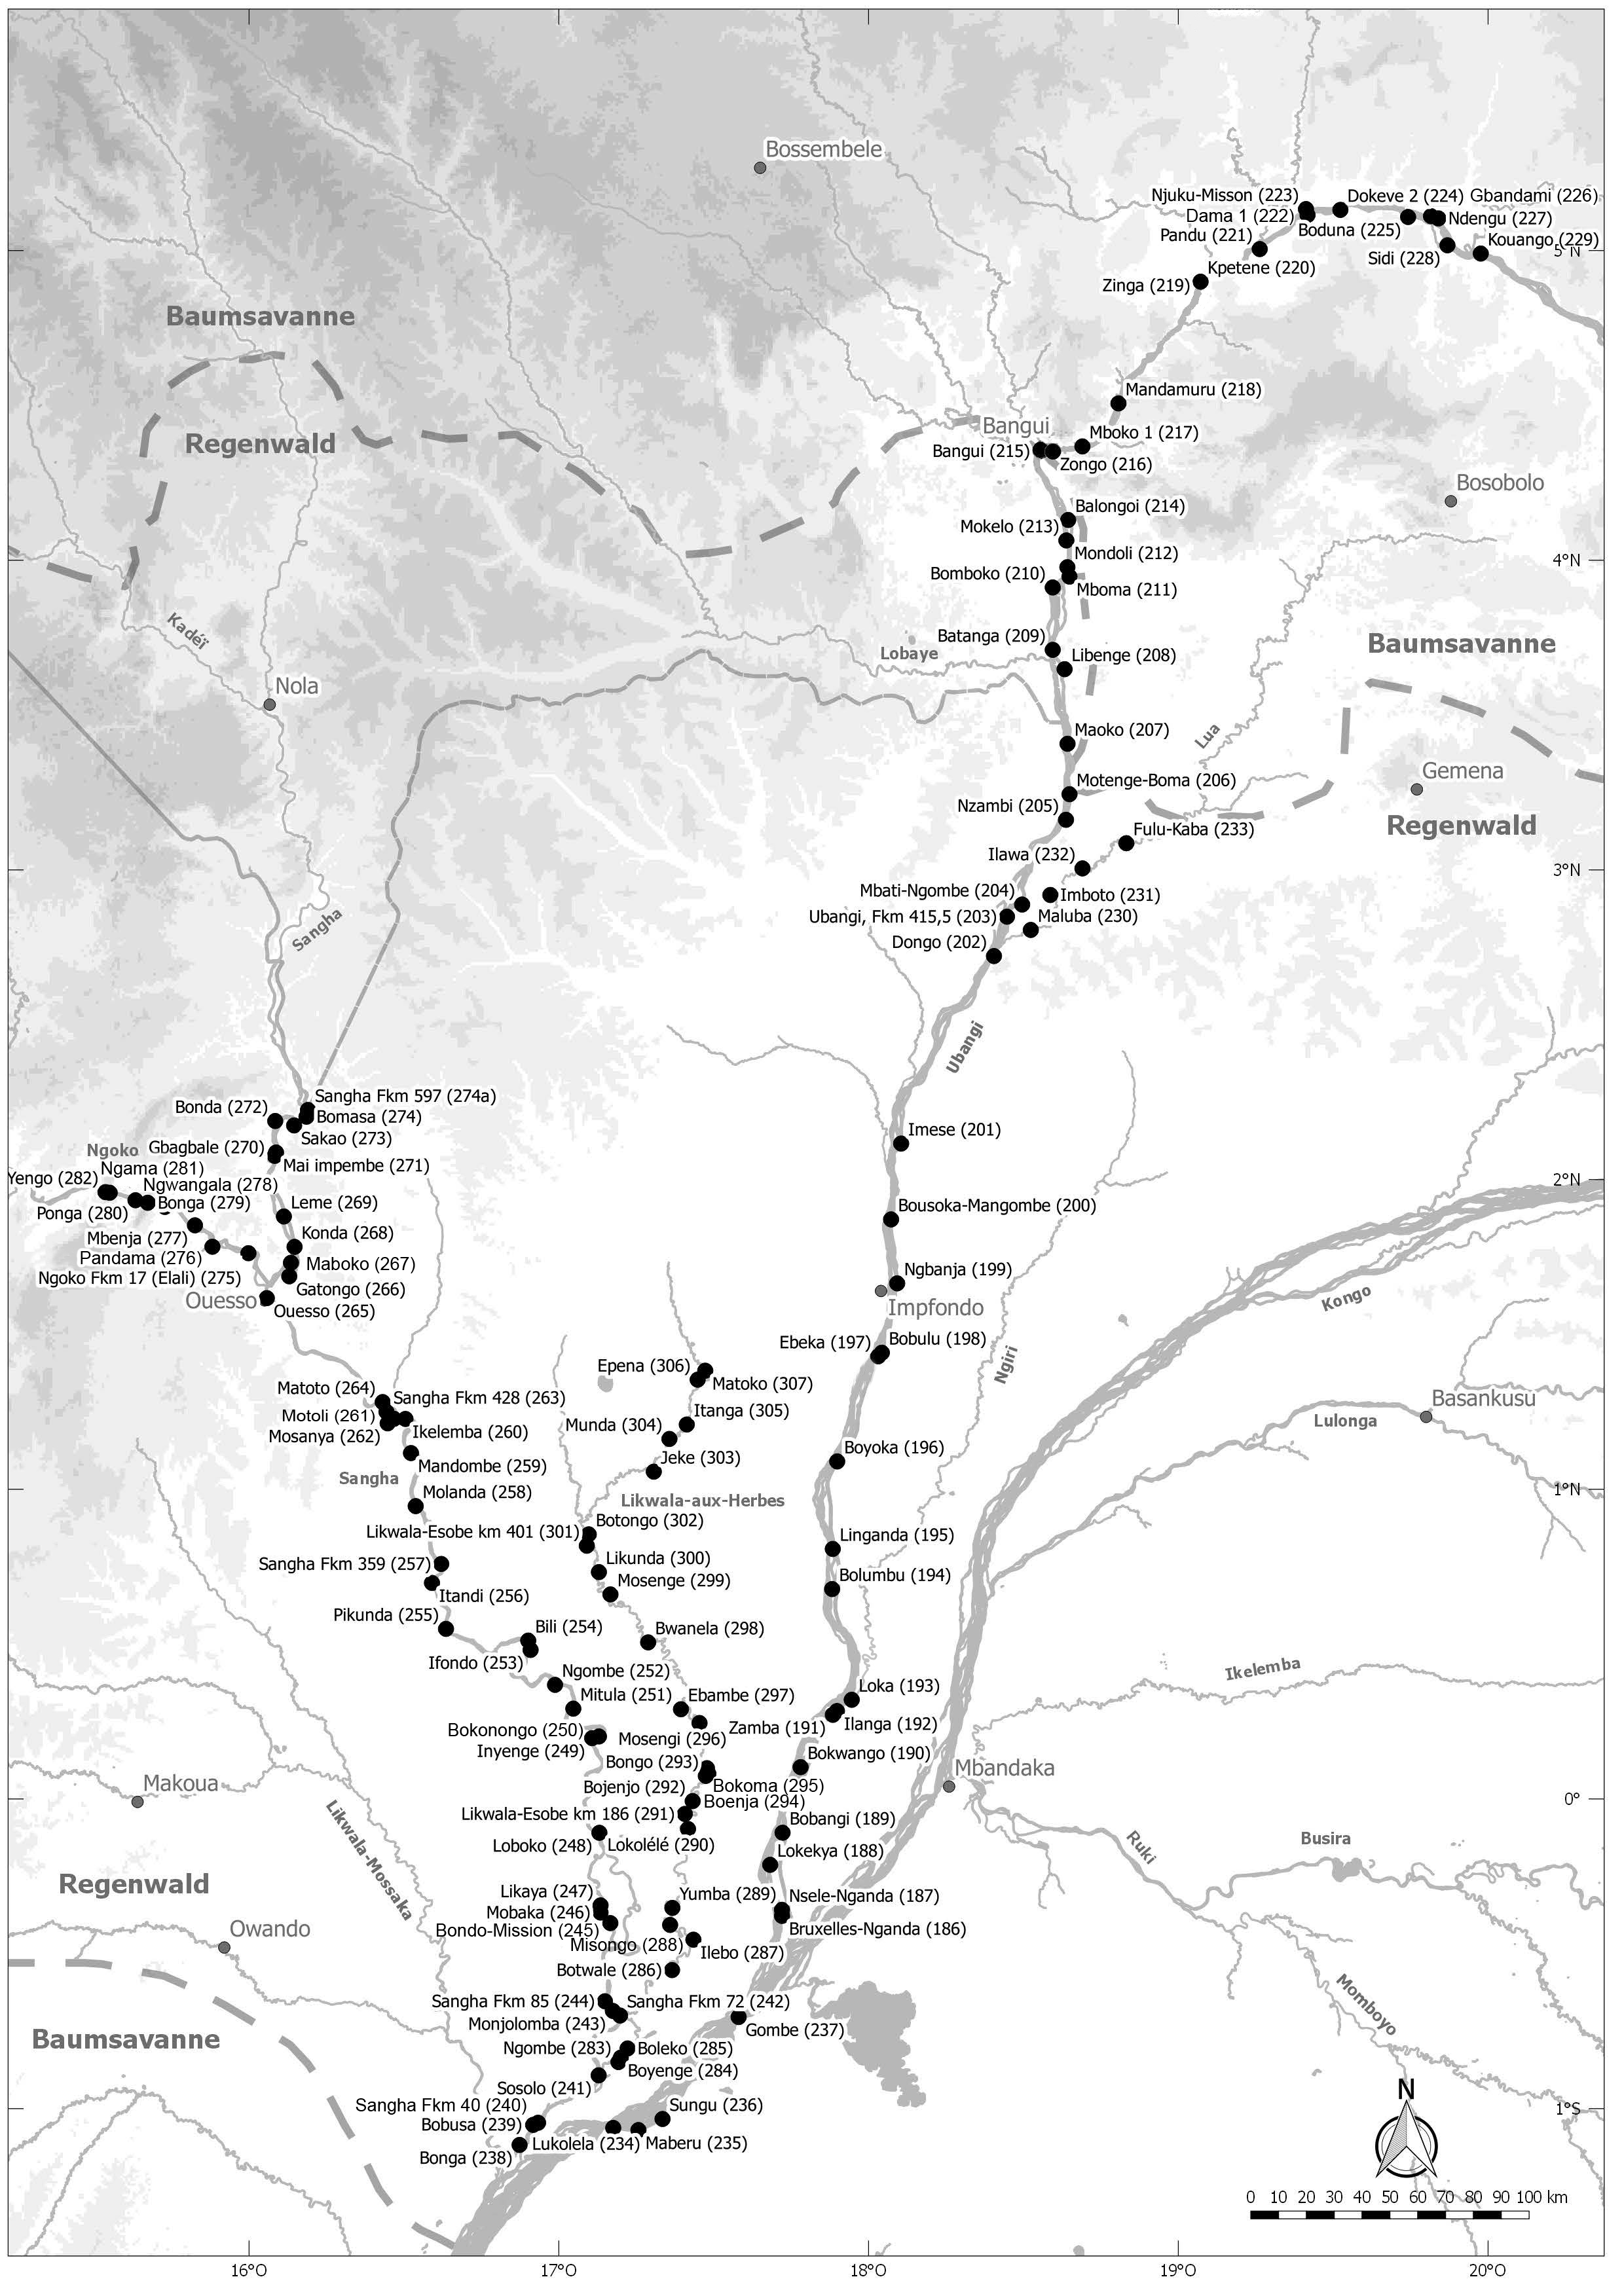
\includegraphics[width=\textwidth]{fig/FundstellenMap.jpg}
	\caption{Arbeitsgebiet: Untersuchte Fundstellen}
	\label{fig:ArbeitsgebietKarte}
\end{figure*}

Das Arbeitsgebiet beschreibt einen Nord--Süd-Transekt von der Feuchtsavanne nördlich von Bangui (Zentralafrikanische Republik) bis in den äquatorialen Regenwald südlich von Mba\-ndaka (Demokratische Republik Kongo). In Nord--Süd-Richtung erstreckt es sich über 700\,km, während es in Ost--West-Richtung annähernd 500\,km groß ist. Alle Fundstellen liegen zwischen 289--390\,m\,ü.\,NN.\footnote{Die Höhen der Fundstellen wurden einem SRTMv3-Datensatz mit einer Grundauflösung von 3 Bogensekunden beziehungsweise etwa 90\,m entnommen (Quelle NASA/USGS; \url{https://earthexplorer.usgs.gov} Zugriff: 04.\,10.\,2014).}

Die Feldarbeiten des \textit{River Reconnaissance Project} in der zweiten Hälfte der Kampagne von 1985 sowie während der Kampagne von 1987 deckten etwa 2130\,km der Flussläufe des \mbox{Ubangi}, Lua, \mbox{Sangha}, \mbox{Ngoko} und \mbox{Likwala}-\mbox{aux}-\mbox{Herbes} ab (Tab.~\ref{tab:ArbeitsgebietFlussstrecken}). Ausgehend von seiner Mündung in den \mbox{Sangha}, die etwa 3\,km nördlich von Ouesso (Fpl.~265) liegt, wurde der \mbox{Ngoko} auf einer Strecke von etwa 80\,km stromauf prospektiert.\footnote{Der untere Abschnitt des Dja, der in Kamerun entspringt, wird ab dem Punkt, an dem er die Grenze zwischen Kamerun und der Republik Kongo bildet (2$^\circ$12$'$25$''$~N, 14$^\circ$35$'$42$''$~O) als \enquote*{\mbox{Ngoko}} bezeichnet. In Yengo (Fpl.~282) musste die Prospektion aufgrund der Malaria-Erkrankung eines Mitarbeiters vorzeitig beendet werden.\label{ftn:DjaNgoko}} Der \mbox{Sangha} bildet den Unterlauf des Kadeï, der in Nordkamerun nahe Garoua-Bouleï entspringt und ab Nola (Zentralafrikanische Republik) als \mbox{Sangha} bezeichnet wird. Der Fluss mündet bei Mossaka, etwa 220\,km südwestlich von Mbandaka in den Kongo. Er wurde auf einer Länge von fast 600\,km bis an das Dreiländereck der Republik Kongo, Kamerun und der Zentralafrikanischen Republik knapp nördlich von Bomasa (Fpl.~274) befahren. Zwischen den Flüssen \mbox{Sangha} und \mbox{Ubangi} liegt der Likwala-aux-Herbes, der auch als \enquote*{Likwala-Esobe} oder \enquote*{Likouala-aux-Herbes} bezeichnet wird und nordwestlich des Lac Tele entspringt. Der \mbox{Likwala}-\mbox{aux}-\mbox{Herbes} wurde insgesamt auf einer Strecke von über 500\,km prospektiert, bis zur nicht passierbaren Brücke bei Matoko (Fpl.~307).\footnote{Der Fluss darf nicht mit dem Likwala-Mossaka verwechselt werden, der auf einigen Karten nur mit der Bezeichnung \enquote*{Likwala} verzeichnet ist. Er verläuft westlich des \mbox{Sangha} und mündet bei Mossaka, wie auch der \mbox{Sangha}, in den Kongo.} Der \mbox{Ubangi} zählt zu den größten Zuflüssen des Kongo und bildet die Grenze zwischen der Demokratischen Republik Kongo und der Zentralafrikanischen Republik sowie der Republik Kongo. Er entspringt aus dem Zusammenfluss von Uele und Mbomou bei Yakoma (Demokratische Republik Kongo) und mündet etwa 90\,km südwestlich von Mbandaka in den Kongo. Der \mbox{Ubangi} wurde auf einer Strecke von etwa 850\,km, bis Kouango (Fpl.~229) befahren. Der Lua ist neben dem Ngiri einer der größten linksseitigen Zuflüsse des \mbox{Ubangi}. Er mündet bei Dongo (Fpl.~202) in den \mbox{Ubangi} und wurde auf einer Strecke von etwa 100\,km bis Fulu-Kaba (Fpl.~233) prospektiert.

\vspace{1.5em}
\noindent Durch diese Feldarbeiten der 1980er Jahre ließen sich für die in dieser Arbeit präsentierte Erstbearbeitung der Befunde und Funde aus dem nordwestlichen Kongobecken eine Reihe von Fragestellungen und Arbeitsziele formulieren:
\begin{itemize*}
\item Die Auswertung der ausgegrabenen Befunde in Maluba (Fpl.~230; Kat.-Nr.~1--5), Bobusa (Fpl.~239; Kat.-Nr.~6--7), Pikunda (Fpl.~255; Kat.-Nr.~8--10), Boleko (Fpl.~285; Kat.-Nr.~14) und Munda (Fpl.~304; Kat.-Nr.~15--18).
\item Die Aufnahme und Auswertung der noch nicht bearbeiten Keramik des \textit{River Reconnaissance Project} aus den Feldkampagnen von 1985 (Flüsse: \mbox{Ubangi} und Lua) und 1987 (Flüsse: \mbox{Sangha}, \mbox{Ngoko} und Likwala-aux-Herbes).
\item Die Formulierung einer Besiedlungsabfolge für die befahrenen Flussläufe des \mbox{Sangha}/\mbox{Ngoko}, \mbox{Likwala}-\mbox{aux}-\mbox{Herbes} und \mbox{Ubangi}/Lua.
\item Ein Vergleich der erarbeiteten archäologischen Sequenz mit benachbarten Regionen, allen voran dem von \textcite{Wotzka.1995} untersuchten Inneren Kongobecken.
\end{itemize*}
\vfill
\noindent\begin{minipage}[b]{\columnwidth}
	{\footnotesize \begin{sftabular}{@{}p{.2\textwidth}R{.2\textwidth}p{.49\textwidth}@{}}
			\toprule
			\textbf{Flusslauf} & \textbf{Befahrung} & \textbf{Endpunkt} \\
			\midrule
			\mbox{Ubangi} & 850\,km & Kouango (Fpl.~229) \\
			Lua & 97\,km & Fulu-Kaba (Fpl.~233) \\
			Kongo/Za{\"i}re & 60\,km & Zwischen Gombe (Fpl.~234) und Lokolela (Fpl.~237) \\
			\mbox{Sangha} & 597\,km & Bomasa (Fpl.~274a) \\
			\mbox{Ngoko} & ca. 80\,km & Yengo (Fpl.~282)\\
			Likwala-aux-Herbes & 526\,km & Matoko (Fpl.~307) \\
			\bottomrule
	\end{sftabular}}
	\captionof{table}{Arbeitsgebiet: Prospektierte Flussabschnitte (siehe Abb.~\ref{fig:ArbeitsgebietKarte})\label{tab:ArbeitsgebietFlussstrecken} \vspace{2.75em}}
\end{minipage}
\noindent Aus diesen Hauptzielen ergaben sich eine Reihe von Kernfragen:
\begin{itemize*}
\item Welche keramischen Stilgruppen lassen sich vor dem Hintergrund der beobachtbaren Variabilität keramischer Formen im Arbeitsgebiet formulieren?
\item Welche Rückschlüsse lassen sich von Eigenschaften sowie Spuren an der Gefäßkeramik auf die Herstellungstechniken herleiten?
\item Welches sind die ältesten im Arbeitsgebiet anzutreffenden keramischen Stilgruppen?
\item Welche relativ- sowie absolutchronologischen Verbindungen bestehen zwischen den einzelnen keramischen Stilgruppen des Arbeitsgebietes?
\item Welche Beziehungen bestehen zwischen den keramischen Stilgruppen des nordwestlichen Kongobeckens und denen der umgebenden Regionen, vor allem dem Inneren Kongobecken?
\item Welche keramischen Stilgruppen des Inneren Kongobeckens können auch im nordwestlichen Kongobecken beobachtet werden?
\item Welche Konsequenzen ergeben sich aus den neu hinzugewonnenen Erkenntnissen aus der Sequenz des nordwestlichen Kongobeckens für die Besiedlungsgeschichte des Kongobeckens allgemein?
\end{itemize*}

\section{Forschungsgeschichte}

\paragraph{Feldforschung vor 1977}\hspace{-.5em}|\hspace{.5em}%
Die Geschichte der archäologischen Erforschung des Kongobeckens bis in die späten 1980er Jahre, mit besonderem Fokus auf das Innere Kongobecken, wurde durch \textsc{Wotzka} (ebd. 22--31) systematisch vorgestellt. Die erste archäologische Ausgrabung im nordwestlich angrenzenden Arbeitsgebiet wurde 1968 durch Roger \textcite{deBayledesHermens.1975} in Batalimo am linken Ufer des Lobaye (Abb.~\ref{fig:BTM-Verbreitung}), einem Zufluss des \mbox{Ubangi}, durchgeführt. Durch einen kleinen Testschnitt von 6\,m\textsuperscript{2} (2\,\( \times \)\,3\,m; ebd. 206--221) wurde in einer \enquote*{Kulturschicht} Keramik sowie Steinartefakte erfasst (\textsc{De Bayle des Hermens} 1975: Taf.~32). Bereits bei der Grabung konnten zwei keramische Gruppen unterschieden werden: flachbodige, reich verzierte Gefäße und einfache, unverzierte Töpfe mit sich leicht verengender Öffnung \parencites[224, 234]{Aumassip.1975}[134]{Eggert.1987c}. Eine dem reich verzierten Material aus Batalimo entsprechende Keramik wurde 1985 auch von \textsc{Eggert} (ebd. 137--141) an der Fundstelle Maluba am Lua (Fpl.~230) entdeckt und in Zusammenschau mit den älteren Funden vom Lobaye unter der Bezeichnug \enquote*{Batalimo-Maluba-Gruppe} subsumiert (siehe Kap.~\ref{sec:BTM-Gr}).

Zwischen Dezember 1972 und März 1973 untersuchte Francis Van Noten in Motenge-Boma am \mbox{Ubangi} (Fpl.~206) eine oberflächlich sichtbare Fundkonzentration von geschliffenen Steinbeilen.\footnote{Im Zuge dieser Feldarbeit wurde durch \textcite[75]{vanNoten.1978} auch eine Testgrabung in der westlich von Gemena gelegenen Höhle Hau durchgeführt. Durch die Grabung wurden drei Schichten erfasst, die sich durch ein jeweils spezifisches Fundinventar auszeichneten. Die unterste Schicht enthielt ein Inventar, das sich durch in Levallois-Technik geschlagene Steinwerkzeuge auszeichnete und vom Ausgräber in die Mittlere Steinzeit datiert wurde \parencite[27, 30]{vanNoten.1982a}. Die darüber liegende mittlere Schicht wies ein mikrolithisches Inventar auf und wurde daher als der Jüngeren Steinzeit zugehörig angesprochen, während die oberste Schicht sich durch potenziell eisenzeitliche Keramik und anderes subrezentes Fundmaterial auszeichnete \parencite[31]{Bahuchet.1992}. Drei, mutmaßlich aus den einzelnen Schichten entnommene Radiokohlenstoffdatierungen ergaben leider lediglich moderne Altersspannen, was für den Ausgräber als Hinweis auf starke Durchmischungen gedeutet wird \parencite[27, 30]{vanNoten.1982a}.} Eine kleine Grabung mit einigen Testschnitten erbrachte aber nur wenig rouletteverzierte und vom Ausgräber in der Folge als \enquote*{eisenzeitlich} angesprochene Keramik (ebd.~58). Die Testschnitte lieferten wenig Material und reichten nicht sehr tief (ebd.~69). Die gefundene Keramik erinnere an Formen aus dem nördlichen Ubangi-Gebiet, unterscheide sich aber vom zeitgenössischen lokalen Material. Jedoch würden moderne, in der Region genutzte hölzerne, geschnitzte Roulettes eine ähnliche Verzierung hervorbringen, wie sie auf den ausgegrabenen Stücken zu sehen sind (ebd.). Eine detaillierte Vorlage der von Van Noten am Fundplatz Motenge-Boma durchgeführten archäologischen Maßnahmen liegt nicht vor, so dass sich über die geschilderten Sachverhalte hinaus keine Angaben machen lassen. Funde, die der von \textsc{Van Noten} (ebd. Abb.~40) präsentierten Keramik entsprechen, wurden auch im hier ausgewerteten Fundmaterial erfasst und unter der Bezeichnung \enquote*{Motenge-Boma-Gruppe} (Kap.~\ref{sec:MTB-Gr}) systematisiert.

\paragraph{Feldforschung des \textit{River Reconnaissance Project} (1977--1987)}\label{sec:RiverReconProjHist}\hspace{-.5em}|\hspace{.5em}%
Der archäologische Forschungsstand im Kongobecken geht fast ausschließlich auf das von der Deutschen Forschungsgemeinschaft geförderte und von Manfred K.~H. Eggert geleitete Regen"-wald-Projekt zurück. Von September 1977 bis Februar 1978 wurden im Rahmen eines ersten Aufenthalts im Ruki-Gebiet, östlich der Provinzhaupstadt Mbandaka erstmals systematisch archäologische Arbeiten in der Äquatorregion der Demokratischen Republik Kongo (ehem. Zaïre) durchgeführt\linebreak \parencites[407--426]{Eggert.1980b}[23\,f.]{Wotzka.1995}. Zwischen 1981--1987 führte das ebenfalls durch die DFG geförderte \textit{River Reconnaissance Project} vier weitere jeweils sechsmonatige Feldaufenthalte mit großräumigen ethnologischen und archäologischen Surveys und Grabungen in der Demokratischen Republik Kongo, der Republik Kongo (ehem. Volksrepublik Kongo) sowie angrenzenden Regionen (Zentralafrikanische Republik und Kamerun) durch. Das Projekt hatte die Untersuchung der Archäologie der großen Zuflüsse des Kongo-Stroms zum Ziel und zusammengenommen wurden etwa 5000 Flusskilometer befahren \parencite[295]{Eggert.1993}.\footnote{Vor allem implizite Annahmen, die dem durch das \textit{River Reconnaissance Project} verfolgten Ansatz von Prospektionen entlang der Flüsse zugrundeliegen, wurde von \textcite[34--36]{Bower.1986} kritisiert. So sei die Auswahl von Fundstellen, an denen Grabungen durchgeführt wurden, lediglich nach mehr oder weniger opportunistischen Kriterien erfolgt (ebd. 35). \textsc{Bower} (ebd.) verweist auch auf die Umstände, dass angesichts des Stands der Auswertung der Grabungen zum Zeitpunkt seiner Kritik Mitte der 1980er Jahre deutliche Unstimmigkeiten zwischen stratigrafischen und auf Radiokohlenstoffdatierungen basierenden chronologischen Rückschlüssen bestanden. Jedoch stand zu diesem Zeitpunkt die detaillierte Auswertung der Befunde und Funde durch \textcite{Wotzka.1995} noch aus; auch die Problematik der im Labor in Hannover vorgenommenen Radiokarbon-Datierungen wurde zwar von M.~K.~H. \textcite[132--133]{Eggert.1987c} mit guten Gründen vermutet und mit dem Laborleiter M.~A. Geyh Mitte der 1980er Jahre diskutiert, jedoch von Letzterem bestritten (pers. Mitt. M.~K.~H. Eggert vom 9. März 2019; siehe Anm.~\ref{ftn:c14Hannover}). Die Schwierigkeiten, eine schlüssige Chronologie zu erarbeiten, gründen folglich nicht auf den von \textcite[36]{Bower.1986} angeführten Grabungen in heutigen Dorfflächen und damit verbundener Durchmischung der Ablagerungen. Der sehr spezifische Naturraum mit starken Überschwemmungen schränkt die zur Besiedlung geeigneten Bereiche im unmittelbaren Uferbereich der Flüsse grundsätzlich stark ein. \textcite[296]{Eggert.1993} verweist auf die immense Fläche, die durch die gewählte zügige Befahrung der Flüsse erschlossen werden konnte. Die Hypothese, dass sich durch die Flussprospektionen auch die Töpfereitraditionen im Hinterland der Flüsse erfassen lassen, wurde 1983 durch eine Moped-Prospektion nördlich von Imbonga am Momboyo (Fpl.~43), die über Land bis an den Salonga und Busira führte, getestet \parencite[18 Anm.~3, 26]{Wotzka.1995}. Diese zusätzliche Prospektion erbrachte keine keramischen Formen, die von \textsc{Wotzka} (ebd. 230) nicht als Teil der \textit{West-Tradition} der \textit{Äquator-Co-Tradition} angesprochen werden konnten. Da diese Prospektion jedoch nur wenige Funde von nicht direkt an Flüssen gelegenen Plätzen erbrachte, muss die in der Auswertung von \textsc{Wotzka} (ebd.) angedeutete Verifizierung der Hypothese, dass die keramischen Inventare aus den Dörfern an den Flüssen ein umfangreiches Bild der Regionalen Entwicklung nachzeichnen, als provisorisch gelten.} Der bisherige Stand der Ergebnisse des Projekts wurde in Form einer umfangreichen Anzahl von Publikationen durch \textcites{Eggert.1980b}{Eggert.1981}{Eggert.1983}{Eggert.1984}{Eggert.1984b}{Eggert.1987}{Eggert.1987c}{Eggert.1992}{Eggert.1993} sowie die umfassende Auswertung der Befunde und Funde aus dem Inneren Kongobecken durch \textcite{Wotzka.1995} veröffentlicht. \textsc{Wotzka} erarbeitete eine umfassende Keramiksequenz für die linksseitigen Nebenflüsse des Kongo-Stromes anhand einer über \enquote{stilistische Bindeglieder geknüpften Kette} (ebd. 65) von Stilgruppen (siehe Kap.~\ref{sec:ICB_StilGrDatierungen}). Die Besiedlungsgeschichte der einzelnen Flussgebiete und letztlich des gesamten Inneren Kongobeckens werden für die vergangenen 2400 Jahre mit archäologischen Methoden nachgezeichnet und ihre Relevanz im Kontext der Bantu-Expansion erörtert.

Die Imbonga-Gruppe beschreibt dabei den frühesten Keramikstil im Inneren Kongobecken (ebd. 65). Die derzeit vorliegenden absoluten Datierungen für den Imbonga-Stil fallen im Kern in den Zeitraum zwischen 400--100 v.~Chr. (ebd. 67, siehe Abb.~\ref{fig:14C_InnerCongo_Stylegroups}). Woher die Menschen gekommen waren, die vor knapp zweieinhalb Jahrtausenden Imbonga-Keramik herstellten und die Äquatorregion der heutigen Demokratischen Republik Kongo besiedelten, ist bis heute ungeklärt, da sich bislang keine direkten Vorläuferstile fanden. Wotzka war jedoch in der Lage, ausgehend von der Imbonga-Gruppe eine stilistische Abfolge bis zu den rezenten Keramikgruppen der Region zu erarbeiten.

Die zweite Hälfte der Kampagne von 1985 führte mit der Prospektion des \mbox{Ubangi} aus dem Inneren Kongobecken hinaus. Zusätzlich zur Prospektion der Flüsse Ikelemba (300\,km), Lulonga (180\,km), Lopori (180\,km) und Maringa (545\,km) konnte der \mbox{Ubangi} auf einer Länge von 800\,km sowie der Lua auf 100\,km Länge prospektiert werden \parencite[129]{Eggert.1987c}.\footnote{Keramik ähnlich jener aus Batalimo \parencites{deBayledesHermens.1975}{Aumassip.1975} wurde bei dieser Prospektion an einer Reihe von Fundstellen entdeckt \parencite[134 Abb.~4; siehe Kap.~\ref{sec:BTM-Gr}]{Eggert.1987c}. Vor allem ein in Dongo am mittleren \mbox{Ubangi} (Fpl.~202) gefundener Komplex erbrachte eine größere Anzahl entsprechender Gefäße (Taf.~9.1--5).} In Maluba am unteren Lua (Fpl.~230) wurden mehrere Gruben entdeckt und ausgegraben (Kat.-Nr.~1--5). Sie enthielten Funde mit starker Ähnlichkeit zur Keramik aus Batalimo, die daraufhin von Eggert als \enquote*{Batalimo-Maluba-Horizont} zusammengefasst wurde (ebd. 138--140; Kap.~\ref{sec:BTM-Gr}).

Die Frage nach den Zusammenhängen zwischen der Keramik aus Batalimo und Maluba mit der aus Imbonga konnte anhand der 1985 vorliegenden Daten nicht gelöst werden (ebd. 141--143). Daher wurde das Untersuchungsgebiet des Projekts nach Westen auf das Gebiet der Republik Kongo und Kamerun erweitert. 1987 wurden die Prospektionen entlang der Flüsse \mbox{Sangha} und \mbox{Likwala}-\mbox{aux}-\mbox{Herbes} sowie entlang des \mbox{Ngoko}, dem Grenzfluss zwischen der Republik Kongo und Kamerun durchgeführt. Die Flussgebiete des \mbox{Sangha}/\mbox{Ngoko} und \mbox{Likwala}-\mbox{aux}-\mbox{Herbes} waren bis zur Feldkampagne von 1987 archäologische \textit{terra incognita} und der Survey erbrachte eine Gruppe charakteristischer Keramikgefäße, die nach den beiden wichtigsten Fundstellen von \textcite[16\,f.]{Eggert.1992} als \enquote*{Pikunda-Munda-Horizont} bezeichnet wurde.

Ein Charakteristikum der Besiedlungsabfolge des nordwestlichen Kongobeckens trat bereits während der Feldarbeiten offen zu Tage: Keramik der frühesten Gruppe des Inneren Kongobeckens, der Imbonga-Gruppe, konnte an keiner Fundstelle in signifikantem Maße beobachtet werden \parencite[4; siehe Kap.~\ref{sec:IMB-Gr}]{Eggert.1987c}. Dies warf die Fragen auf, mit welcher Keramikgruppe die Sequenz im nordwestlichen Kongobecken beginnt, woher diese Keramik stammt und ob es Verbindungen zur Imbonga-Keramik des Inneren Kongobeckens gibt. Deutlich war, dass die ursprüngliche Besiedlung nicht vom nordwestlichen Kongobecken aus in das Innere Kongobecken hinein erfolgte, sondern dass die Herkunft der Imbonga-Keramik woanders gesucht werden muss \parencite[257 Anm.~49]{Wotzka.1995}.

Die Auswertung des Fundmaterials aus dem Inneren Kongobecken wurde 1990 durch Hans-Peter Wotzka als Promotionschrift an der Universität Hamburg vorgelegt und 1995 veröffentlicht.\footnote{Die Materialien aus der zweiten Hälfte der Feldkampagne von 1985 sowie jene von 1987 blieben in \textsc{Wotzkas} (1995) Auswertung unberücksichtigt. Er konnte die Funde allerdings in Augenschein nehmen und in Form kurzer Verweise auf Details eingehen (ebd. 29, 68, 107, 119, 139, 270--272). Während \textsc{Wotzka} (ebd. 227 Tab.~114, 392, 450--452 Taf. 16--18) die Keramik des Fundplatzes Bamanya im westlichen Hinterland des Ruki (Fpl.~12) in seine Untersuchungen einschloss, unterbliebt die Aufarbeitung der Befunde (ebd. 138 Anm.~17; 310). Weder die Arbeit von Wotzka noch die vorliegende Auswertung behandeln die Befunde und Funde, die im Zuge der Ausgrabung in einem Grabenwerk in Mondjo am Ikelemba (Fpl.~133) erschlossen wurden \parencite[3238--3240]{Eggert.1987}.} Die 1985 und 1987 im nordwestlichen Kongobecken gemachten Funde wurden -- noch in Hamburg -- beschriftet und in einer umfangreichen Auswahl gezeichnet.\footnote{Eine zweite Auswahl Keramik wurde, nach der Berufung des Projektleiters M.~K.~H. Eggert als Professor nach Erlangen und später Tübingen, in einer Kombination aus gezeichneten Profilen und fotografierten Ansichten als Tafelabbildungen vorbereitet.} Nach dem Ende der Feldarbeiten erfolgten einzelne Arbeitsschritte zur Auswertung des Fundguts aus dem nordwestlichen Kongobecken. So wurden Kurzbeschreibungen der Befunde sowie Funde angefertigt und eine erste formale Ansprache der Gefäßkeramik vorgenommen.

\paragraph{Feldforschung nach 1987}\label{sec:FeldforschModern}\hspace{-.5em}|\hspace{.5em}%
Zwischen dem Ende der Feldarbeiten des \textit{River Reconnaissance Project} im Jahr 1987 bis zum Beginn der 2010er Jahre erfolgte im Arbeitsgebiet aufgrund politischer Instabilitäten und damit verbundener prekärer Sicherheitslage praktisch keine archäologische Feldforschung. Die Feldarbeiten des \textit{River Reconnaissance Project} fanden Ende der 1990er Jahre ihre Fortführung im Südosten der Republik Kamerun (\textsc{Eggert} 2002; Kap.~\ref{sec:Kamerun}).\footnote{Die Ergebnisse dieser Feldarbeiten sind bislang nicht umfassend aufgearbeitet und vorgelegt.}

Im Südwesten der Zentralafrikanischen Republik, vor allem aber der Region um die Hauptstadt Bangui, wurden seit den 1990er Jahren verschiedentlich archäologische Fundstellen neu erschlossen. Vornehmlich handelt es sich um Prospektionsaktivitäten, die vor ethnoarchäologischen Fragestellungen durchgeführt wurden und im Rahmen von Qualifikationsschriften an der Universität von Bangui \parencites{Ndanga.199596}{Abrou.199697} oder in Frankreich \parencites{Kote.1992}{Scouflaire.1997} ausgewertet wurden. Die Arbeiten lieferten zwar durchaus neue Datierungen, fanden aber nur selten Eingang in überregionale Synthesen zur Besiedlungsabfolge. Weitere Arbeiten widmeten sich der Metallurgiegeschichte in der Region und verfolgten dabei ebenfalls vornehmlich ethnoarchäologische Forschungsansätze \parencites{Muramira.20042005}{Muramira.20052006}{Moga.2008}. In den Jahren 2008 bis 2010 wurden durch Jean-Paul Ndanga neue Grabungen in Batalimo am Lobaye sowie der 1,5\,km entfernt liegenden Fundstelle Ngo Tchororo durchgeführt \parencite{Ndanga.2010}.\footnote{Die Arbeiten wurden 2010 durch Els Cornelissen und Raymond Lanfranchi unterstützt. Eine systematische Auswertung der Befunde und Funde steht aufgrund der politischen Instabilität innerhalb der Zentralafrikanischen Republik gegenwärtig leider aus (pers. Mitt. E.~Cornelissen vom 06.10.2016; siehe auch Kap.~\ref{sec:BTM-Gr}).}

Die seit den 2010er Jahren in der Region durchgeführten Forschungsvorhaben mit internationaler Beteiligung verfolgten häufig paläo-ökologisch-archäologische Forschungsansätze \parencites[siehe][]{Kiahtipes.2011}{Gillet.2013}{MorinRivat.2014}{Kiahtipes.2016}. Im Jahr 2011 wurden durch die Arbeitsgruppe um Karen Lupo ausgedehnte archäologische und paläo-ökologische Prospektionen sowie kleinere Testschnitte im Umfeld des Fundplatzes Bagbaya in der südwestlichen Zentralafrikanischen Republik angelegt \parencite{Lupo.2015}.\footnote{Der Ortsname \enquote*{Bagbaya} lässt sich mit \enquote{Eisenmarkt} übersetzen (\textsc{Lupo} 2015: 3). Neben zwei offenen Abbaugruben für Eisenerz wurden 18 etwa 1,5 bis 2\,m hohe sowie 15 flachere in die vorkoloniale Zeit datierende sowie einige ältere Schlackehügel entdeckt (ebd. 6 Tab.~1, 8). Bei den in den beiden untersuchten Abbaugruben gewonnen Erzen handelt es sich um eisenreiche Ablagerungen jener mafischen Basalte, die in der unmittelbaren Umgebung anstehen (ebd. 6). Insgesamt elf der prospektierten Schlackehügel wurden durch kleine, 1\,$\times$\,1 oder 1\,$\times$\,2\,m große Testschnitte näher untersucht (ebd. 8). Bei den in den Testschnitten gefundenen Schlacken handelt es sich um blasige Fließschlacken, die als primäre Verhüttungsschlacken angesprochen werden (ebd. 10). Die Bedeutung einiger der Schlackehügel als Anzeiger für Eisengewinnung war der lokalen Bevölkerung sehr gut bekannt, wie mündliche Befragungen ergaben (ebd.).} Konkrete Verhüttungsbefunde im Sinne von Öfen wurden nicht erfasst. Die Ausgräber interpretieren ihre Ergebnisse sehr weitreichend als Zeichen eines vorkolonialen, regionalen Handelsnetzes, das bis in die ethno-historische Zeit reichte (ebd.~2). Zusammen mit den archäologischen Arbeiten wurden paläo-ökologische Untersuchungen durchgeführt.

Neben dem Südwesten der Zentralafrikanischen Republik rückte der Norden der Republik Kongo, auch durch umfangreiche Konzessionen für Holzeinschlag \parencites[siehe][Abb.~S3]{Gond.2013}[166 Abb.~1]{Brandt.2016}, und vor allem die Region des \mbox{Sangha} vermehrt in den Fokus der Forschung. Während Veröffentlichungen die neu gewonnenen Radiokohlenstoffdatierungen \parencite{Oslisly.2013b} sowie Erkenntnisse aus paläobotanischen Proben \parencite{MorinRivat.2014} umreißen, fehlt bislang jedoch die Vorlage des archäologischen Fundguts. Lediglich von der am \mbox{Sangha}, etwa 25\,km südöstlich von Ouesso (Fpl.~265) gelegenen Fundstelle Mboua Mboua und dem 65\,km südöstlich von Mboua Mboua gelegenen Ort Ibamba sowie zwei unbenannten Stellen, die sich etwa 70\,km nördlich von Mboua Mboua befinden (siehe Abb.~\ref{fig:PIKMUN_Verbreitung}), sind einige wenige Keramikformen bekannt \parencite[95 Abb.~31, 114 Abb.~42]{Gillet.2013}. Das Material kann teilweise in die im Rahmen der vorliegenden Untersuchung erarbeitete Stilgruppen-Sequenz der Region integriert werden (siehe Kap.~\ref{sec:SequenzSanghaNgoko}).

Auch außerhalb des eigentlichen Arbeitsgebietes setzte erst zu Beginn der 2010er Jahre wieder erste archäologische Feldforschung ein. Die Region entlang des nördlichen Kongobogens, der Mündungsbereich der Flüsse Itimbiri, Aruwimi und Lomami in den Kongo, wurde 2010 erstmals im Rahmen des \textit{\mbox{Boyekoli} \mbox{Ebale} \mbox{Congo}}-Projektes durch Wissenschaftler verschiedener Disziplinen des \textit{Musée royal de l'Afrique centrale} in Tervuren -- auch mit Blick auf die Archäologie -- prospektiert \parencite{LivingstoneSmith.2011}.\footnote{Siehe Kap.~\ref{sec:NordCongo} mit Anm.~\ref{ftn:BoyekoliEbaleCongo}.} Insgesamt wurden sechs Fundstellen erschlossen. Bei Grabungen in Bomane-Yangwa am Aruwimi wurden zwei Gruben näher untersucht. Einer der Befunde enthielt ein umfangreiches keramisches Inventar \parencite[ebd. 13 Abb. 2; ][5 Abb.~3]{LivingstoneSmith.2017}. Die enge, mit einer Vielzahl von Gefäßen verfüllte Grube erinnert dabei sehr an Keramikdeponierungen in Gruben im Inneren Kongobecken \parencite[siehe][256--264]{Wotzka.1993}. Ein sehr ähnlicher Befund wurde auch in Baombi am Lindi aufgedeckt \parencites[78--79 Abb.~5--6]{Cornelissen.2013}[8 Abb.~10]{LivingstoneSmith.2017}. In der Zusammenschau ergab sich eine aus drei Phasen bestehende keramische Sequenz, deren ältestes Element durch die Keramik der beiden genannten Fundstellen repräsentiert ist und in das 4.~Jh. v.~Chr. bis 1.~Jh. n.~Chr. datiert (ebd. 16--19, 17 Abb.~23). Sie ist somit grundsätzlich zeitlich parallel mit der frühesten, durch die Keramik der Imbonga-Gruppe (Kap.~\ref{sec:IMB-Gr}) repräsentierte Besiedlung des Inneren Kongobeckens \parencite[65]{Wotzka.1995}. Die folgende \enquote{mittlere Keramikphase} datiert vom 1.--6.~Jh. n.~Chr., während die jüngere Phase zwischen das 8.--17.~Jh. n.~Chr. anzusetzen ist. Die Keramik der jüngeren Phase zeichnet sich unter anderem durch die Nutzung von Rouletteverzierungen aus (siehe Kap.~\ref{sec:Zeitscheiben}).

Im Jahr 2010 wurden neue Feldarbeiten im Inneren Kongobecken durch Hans-Peter Wotzka initiiert. Im Zuge dieser ersten Anknüpfungen an die Feldarbeiten des von Eggert geleiteten Regenwald-Projektes durch Wotzka wurde auch eine Kiste mit Bodenproben, welche seit 1987 in der Missionsstation in Bamanya nahe der Provinzhauptstadt Mbandaka eingelagert gewesen war, nach Deutschland überführt. Das Probenmaterial sowie ein ähnlich umfangreicher Bestand, der in Tübingen eingelagert war, wurde daraufhin archäobotanisch untersucht. Im Ergebnis dieser Untersuchung konnten erstmals archäobotanische Daten für das Innere Kongobecken vorgelegt werden \parencite{Kahlheber.2014}. Unter anderem fanden sich in Proben aus einer Grube in Boso-Njafo am Lulonga (Fpl.~149) Reste von Perlhirse (\textit{Pennisetum glaucum}), die in die Imbonga-Zeit datieren.\footnote{Siehe \textcites{Wotzka.2019}{Wotzka.2019a} zu den Ergebnissen eines Anbauexperiments von Perlhirse im heutigen Regenwaldgebiet.} In einer Probe aus der Grube MUN~87/2-1-3 in Munda am Likwala-aus-Herbes (Fpl.~304; Kat.-Nr.~17) fand sich ein gut erhaltener Samen der Raphia-Palme (ebd. 506, 508 Abb.~7). Mit Jahresbeginn 2015 begann unter der Leitung von Wotzka ein von der DFG finanziertes Projekt, welches sich gemeinsam mit einem von Katharina Neumann geleiteten Botanik-Projekt die Erforschung von Paläoumwelt und Subsistenzbasis im Inneren Kongobecken während der Eisenzeit zum Ziel gesetzt hat.


\section{Archäologie und Historische Linguistik}

Ein zentraler Forschungsgegenstand der Kulturgeschichte Afrikas südlich der Sahara ist die Ausbreitung \enquote*{Bantu} sprechender Gruppen über fast den gesamten Raum südlich des Äquators: die sogenannte \enquote*{Bantu-Expansion}. Bantu ist eine Sprachfamilie\footnote{Zur gegenwärtig auch in der Forschung anzutreffenden \enquote*{Verschmelzung} von Sprache, Kultur, Gesellschaftsformen sowie \enquote*{Rasse} im Kontext der \enquote*{Bantu}-Sprachen siehe \textcite[302]{Eggert.2005}.}, der zwischen 300 und 680 einzelne Sprachen zugeordnet werden \parencites{Nurse.2003}[81]{Eggert.2016c}. Die hypothetische Urheimat dieser Sprachfamilie wird derzeit im Grenzgebiet von Kamerun und Nigeria -- am nordwestlichen Rand ihrer heutigen Verbreitung -- verortet \parencites[57, Abb.~2]{Pakendorf.2011}[207 Abb.~6a/b]{Eggert.2012}[630 Abb. 43.2]{deMaret.2013}.\footnote{Die Frage nach der Ausbreitung der Bantu-Sprachen im südlichen Afrika wurde über Jahrzehnte im Spannungsfeld von Linguistik und Archäologie diskutiert. Die Debatte wies jedoch bereits früh eine starke Vermischung linguistischer und archäologischer Argumente auf, was deutliche Zirkelschlüsse zur Folge hatte \parencites{Eggert.1981}{Eggert.2005}[82]{Eggert.2016c}. Die seit einigen Jahren hinzukommenden Daten aus populationsgenetischen Untersuchungen führten nicht zu einem Aufbrechen dieses Dilemmas. So lassen sich auf genetischer Seite nur vertikale Vererbungen von Eltern zu Kindern nachvollziehen, während Sprachgemeinschaften, deren Untersuchung angestrebt ist, auch horizontale Beeinflussungen zulassen (ebd. 86). Aus diesem Umstand ergibt sich für \textcite{Eggert.2016c} eine Ausweitung des ursprünglichen Dilemmas zu einem Trilemma. Siehe auch \textcite{Horsburgh.2015} zum Spannungsfeld der Interpretation molekularbiologischer Erkenntnisse in kulturhistorischen Fragestellungen.\label{ftn:LinguistikTrilemma}} Zur Erklärung der Ausbreitung der Bantu-Sprachen postulieren nicht wenige Studien mehr oder minder großräumige Wanderungsbewegungen \parencites{Vansina.1995}{Ehret.2001}. Für das nordwestliche Kongobecken wurden eine Reihe linguistisch inspirierter historischer Hypothesen diskutiert \parencite[10\,f.]{Eggert.1992}. So ging \textcite{Ehret.1982} von einer sehr frühen Besiedlung des Regenwaldes durch Bantu-Sprecher aus. Basierend auf Überlegungen von \textcite{Heine.1973} datierte er die frühesten Phasen der Bantu-Expansion in den zentralen Teil des Regenwaldes -- auch in das gesamte Areal westlich des mittleren und unteren \mbox{Ubangi}-Flusses -- bereits in den Beginn des zweiten vorchristlichen Jahrtausends \parencite[58, 63~Karte 10]{Ehret.1982}. Für \textcite[51\,f. Karten~2.7--2.8]{Vansina.1990} hingegen stellten die weiten Sumpfgebiete westlich des \mbox{Ubangi} eine Barriere für die Ausbreitung der Bantu-Sprecher dar. Er postuliert eine nördliche Ausweichbewegung der allgemein nach Osten gerichteten Ausbreitung des Bantu entlang der nördlichen Grenze des Regenwaldes und lässt die \mbox{Sangha}-Region undatiert (ebd. 51 Karte~2.7).

Eine neuere Synthese linguistischer, paläo-ökologischer sowie archäologischer Daten von \textcite{Bostoen.2015} schließt auf eine Besiedlung des äquatorialen Regenwaldes durch das sogenannte \enquote{\mbox{Sangha}-River-Interval}\footnote{Siehe Anm.~\ref{ftn:SanghaIntervall}.}, eine etwa 400\,km breite Region zwischen 14$^\circ$ und 18$^\circ$ östliche Länge und misst dem südlichen Abschnitt des hier untersuchten Raumes eine zentrale Bedeutung bei. Während die linguistischen Schlüsse für diese Hypothese mit einer grundsätzlich ähnlich gerichteten Studie aus dem gleichen Jahr \parencite{Grollemund.2015} zusammenfallen, werden in der Arbeit von \textcite{Bostoen.2015} keine neuen archäologischen oder paläo-ökologischen Daten aus der Region des \mbox{Sangha}-Flusses vorgestellt.\footnote{Bestehende Quellen zum archäologischen Forschungsstand der Region fanden nur sehr begrenzt Einzug. Die ursprüngliche Veröffentlichung der archäologischen Funde aus der \mbox{Sangha}-Region \parencite{Eggert.1992} wird nicht erwähnt, obschon hier die Keramik der Pikunda-Munda-Gruppe (Kap.~\ref{sec:PKM-Gr}), der ältesten Stilgruppe entlang des unteren \mbox{Sangha}, sowie die zugehörigen Radiokohlenstoffdatierungen im Mittelpunkt stehen. Eine zentrale Veröffentlichung von \textcite{Eggert.1993}, die einen klaren Einblick in die ältesten archäologischen Zeugnisse im \mbox{Sangha}-Gebiet bietet, wird von \textcite{Bostoen.2015} auch nur randlich berücksichtigt. \textsc{Bostoen} u.a. (2015: 356 Abb.~1) verzeichnen lediglich die Fundstelle Imbonga im gesamten Kongobecken. Damit vermitteln die Autoren einen deutlich falschen Eindruck von der archäologischen Quellenlage der Region.} \textsc{Bostoen} u.a. (2015: 355; 362; 364) sehen in Keramik nicht nur eine \enquote{archäologische Signatur der Ausbreitung der Bantu-Sprachen}, die Autoren versuchen auch auf Basis der archäologischen Zeugnisse aus dem Gebiet der Atlantikküste, von Südkamerun bis in den Niederkongo, auf die Vorgänge in der \mbox{Sangha}-Region rückzuschließen. Daneben beziehen sich \textsc{Bostoen} u.a. (2015: 355--358) auf die naturräumlichen Veränderungen innerhalb Zentralafrikas, können jedoch wieder keine neuen Daten präsentieren. Die ungeprüfte Projizierung von eindeutig mit pleistozänen oder frühholozänen Veränderungen des Ökosystems in Zusammenhang stehenden Eigenheiten von Flora und Fauna im Regenwald sowie der Savannenbereiche Zentralafrika auf die \enquote{Regenwaldkrise im 1.~Jt. v.~Chr.} (siehe Kap.~\ref{sec:Palaeoumwelt})\footnote{Siehe hierzu die nach der Fertigstellung der Arbeit erschienene Studie von \textcite{Bremond.2017}, die in einer kombinierten Analyse von Phytolithen und Delta-13C keine Signatur einer Öffnung des Regenwaldes erkennen kann und bei der es sich um die einzige in dieser Region durchgeführte Untersuchung handelt.\label{ftn:Bremond2017}} lässt sich ohne konkrete Daten aus der Region nicht nachvollziehen. \textcite{Bostoen.2015} präsentieren eine mittels eines phylogentischen Stammbaums auf statistischem Wege erzielte Ordnung von 168 modernen Bantu-Sprachen im westlichen Zentralafrika. Eine durch die von \textcite{Bostoen.2015} beteiligten Linguisten im selben Jahr veröffentlichte Arbeit \parencite{Grollemund.2015} präsentiert einen phylogentischen Stammbaum, der auf Daten zu 424 Bantu-Sprachen sowie ähnlichen Sprachen basiert und aus 100 stichprobenartig ermittelten Stammbäumen ausgewählt wurde (ebd.~13297). Die Autoren gehen in dieser Arbeit sogar so weit, dass sie spezifische Knotenpunkte dieses Stammbaums mit archäologischen Datierungen zeitlich \enquote*{kalibrieren}. Hier wird ein direkter Bezug zwischen isolierten archäologischen Phänomenen, wie der Befundlage an der Fundstelle in Shum Laka oder jener in Obobogo (siehe Kap.~\ref{sec:Kamerun}) und statistischen Ergebnissen hergestellt, der methodisch nicht fundiert ist. Darüber hinaus unternehmen \textcite{Grollemund.2015} den Versuch, die geographische Position der durch archäologische Zeugnisse mutmaßlich chronologisch erfassten Knotenpunkte zu ermitteln. Hierdurch wird jedoch eine Ortsfestigkeit der Sprachgruppen implizit vorausgesetzt, die nicht auf Übereinstimmungen mit historischen Überlieferungen abgeprüft wird.\footnote{Siehe beispielsweise die Arbeit von \textcite[83]{Vennetier.1963}, der die oral tradierten Migrationen im Norden der Republik Kongo nachzeichnet.} Aus diesen hypothetischen Ursprungsgebieten leiten die Autoren ein Modell der Ausbreitung der Bantu-Sprachen ab und lediglich im Appendix räumen sie ein, dass das präsentierte Modell mit gerade genug Einschränkungen versehen wurde, um eine \enquote*{Ausbreitung} durch den postulierten \mbox{Sangha}-Korridor zu erzeugen \parencite[SI 3]{Grollemund.2015}. Die geschilderten neueren Arbeiten von \textcite{Bostoen.2015} und \textcite{Grollemund.2015} lassen mit Blick auf implizite Annahmen und direkten Verknüpfungen von archäologischen Zeugnissen und statistischen Resultaten der Historischen Linguistik starke Parallelen an die zirkulären Argumentationen bei \textcites{Phillipson.1976}{Phillipson.1976b}{Phillipson.1977a} und \textcite{Ehret.1973} sowie \textcites{Heine.1973}{Heine.1977} erkennen.\footnote{Siehe \textcites{Eggert.1981}[308\,f.]{Eggert.2005} sowie Anm.~\ref{ftn:LinguistikTrilemma}. Eine detaillierte Beschreibung des Besiedlungsgangs und damit Falsifizierung der Thesen von \textcite{Bostoen.2015} ist gegenwärtig in Vorbereitung.}

Dessen ungeachtet sind die Regenwaldgebiete Zentralafrikas vor allem deshalb von zentraler Bedeutung für die Annäherung an das Problem der Ausbreitung der Bantusprachen, ja geradezu \enquote{der entscheidende Prüfstein für die Rolle der Archäologie bei der Bantuausbreitung} \parencite[207]{Eggert.2012}, da sie aktuell fast vollständig von Bantu sprechenden Gruppen besiedelt sind und die Aufsiedlung durch keramikherstellende Gruppen im Inneren Kongobecken bereits plausibel mit der Bantu-Ausbreitung verknüpft wurde \parencite[244--246]{Wotzka.1995}. Beim gegenwärtigen Stand der archäologischen Erforschung Zentralafrikas müssen jedoch grundsätzlich alle Versuche, die historische Verbreitung beziehungsweise Ausbreitung kulturell-linguistischer Gruppen zu erfassen, als Spekulation bezeichnet werden \parencite[105]{Boyd.2007}. Weder die Historische Linguistik, noch die Populationsgenetik sind in der Lage, Aussagen zur zeitlichen Dimension der jeweils beobachteten Phänomene zu machen \parencite[84]{Eggert.2016c} -- dies vermag lediglich die Archäologie.\footnote{Umfassende kritische Auseinandersetzungen zum Spannungsfeld von Historischer Linguistik und Archäologie in der Frage der Bantu-Expansion finden sich bei \textcites{Eggert.2005}{Eggert.2012}{Eggert.2012c}{Eggert.2016c}.}


\section{Geologie und Böden}

Das Arbeitsgebiet umfasst den nordwestlichen Rand des Kongobeckens, jenem intrakontinentalen Becken, das zirka 1,2 Millionen km\textsuperscript{2} groß ist und den Großteil des Kongokratons, einer der vier tektonisch stabilen Schildregionen Afrikas, einnimmt \parencites[16]{Runge.2001}[240]{KadimaKabongo.2011}. Im Kongobecken, auch als \textit{Cuvette centrale} bezeichnet, ist das präkambrische Grundgebirge von bis zu 3\,km mächtigen, phanerozoischen Sedimentpaketen überlagert. Lediglich in den randlichen Schwellenregionen steht es an der Oberfläche an \parencite[17]{Runge.2001}.\footnote{Diese aus dem Archaikum (4--2,5\,Ma) sowie Paläoproterozoikum (2,5--1,6\,Ma) stammenden Blöcke sind: der \enquote{Zentrale Kasai-Kongo-Block} im südlichen Teil der Demokratischen Republik Kongo (DRC) und Nord-/Zentral-Angola, der \enquote{Kongo-Uganda-Block}, der vom nordöstlichen Teil der DRC in den Süden der Zentralafrikanischen Republik (RCA) und des Sudans [heute Südsudan] und den Osten Ugandas reicht sowie der \enquote{Kamerun-Gabun-Kongo-Block}, der in Kamerun als \enquote{Ntem-Komplex} und in Gabun sowie der Republik Kongo als \enquote{Chailu-Block} bekannt ist \parencite[240]{KadimaKabongo.2011}. Die als Hauptwasserscheiden fungierenden, das Kongobecken umgebenden Grundgebirgsschilde bestimmen das zirka 3,7 Millionen km\textsuperscript{2} große Einzugsgebiet des Kongo, der mit einer mittleren Abflussmenge von etwa 40\,000\,m\textsuperscript{3}/s nach dem Amazonas zu den größten Flüssen der Erde zählt \parencite[63]{Runge.2001}.}  Die geologische Geschichte des Kongobeckens lässt sich in Grundzügen wie folgt zusammenfassen \parencite[313]{Giresse.2005b}:\footnote{Die nach-paleozoische Geologie des Kongobeckens kann gegenwärtig nur auf Basis von zwei Magnetikprofilen sowie geologischen Bohrungen, die zwischen 1973 und 1981 südöstlich von Mbandaka angelegt wurden \parencites[siehe][]{Daly.1991}{Daly.1992}, rekonstruiert werden \parencite[301\,f.]{Giresse.2005b}.} Die Anhebung der Becken-Ränder am Beginn des Känozoikums beendete eine Phase mariner Einbrüche in ein lakustrin oder lagunal geprägtes Milieu. Während die jüngere Geologie des Kongobeckens von verlehmten Sanden und weichen Sandsteinen in nahezu horizontaler Schichtung bestimmt ist (ebd. 302, 303 Abb.~2), führte ein Erosionsereignis am Ende des Tertiär zur teilweisen Verlagerung älterer Ablagerungen (ebd. 306). Im Laufe des Paläogen bestimmen Pakete aus äolischen Ablagerungen, die \textit{Grès Polymorphes Séries}, die Becken-Sedimentation. Der Beginn der bis heute andauernden fluvialen Ablagerungsphase im Kongobecken, die mit verstärkter ferralithischer Bodenbildung einhergeht, lässt sich frühestens mit den neogenen Ablagerungen der \textit{Sables Ocres Séries} in Zusammenhang bringen. 

Das Arbeitsgebiet gliedert sich geologisch folgendermaßen:\footnote{Die Koordinaten der Fundstellen ließen sich auf eine Übersichtskarte der geologischen Grundeinheiten Afrikas \parencite{Persits.2002} projizieren. 71\,\% aller bearbeiteten Fundstellen liegen demnach auf holozänen (Qe), 20\,\% auf präkambrischen Ablagerungen (pCm), 7\,\% im direkten Fluss-Bereich (H20) und 2\,\% sind auf känozoischen Ablagerungen (QT) zu finden.} nördlich von Libenge am \mbox{Ubangi} (Fpl.~208) befinden sich die Fundstellen vornehmlich auf präkambrischen Formen, während die Fundstellen weiter südlich auf den jüngeren, känozoischen und holozänen Ablagerungen liegen, welche das gesamte Kongobecken bestimmen. In nordwestlicher Richtung wurde diese geologische Grenze des Kongobeckens mit den Surveys nur knapp überschritten. Lediglich die wenigen Fundstellen am \mbox{Sangha}, die flussaufwärts von Gbagbale (Fpl.~270) liegen, befinden sich nicht mehr auf jüngerem, holozänem Untergrund. 

Bei den im Arbeitsgebiet angetroffenen Böden handelt es sich zu großen Teilen um Ferralsole. Diese, auch als Oxisole bezeichnete Form der Bodenbildung, zeichnet sich durch eine charakteristische, auf Goethit hinweisende, gelblich bis leicht rötliche Färbung des Unterbodens aus \parencites[351\,f., 355 Abb.~7.6-4]{Scheffer.2010}[144]{Jones.2013}. Dieser wird lediglich von einem dünnen, dunklen und humus-reichen Oberboden überdeckt. Aufgrund von Erosion im Bereich der Dörfer steht der Oberboden dort vielfach nicht mehr an. Ferralsole sind die typische Ausprägung der Pedogenese in den sauren, stark verwitterten Böden der inneren, immerfeuchten Tropen \parencite[27]{Scheffer.2010}.\footnote{Die in Abhängigkeit des Milieus ablaufende Substitution von Eisen (Fe) durch Aluminium (Al) ist im sauren Milieu der Tropen deutlich höher als in neutralen oder reduzierenden Böden (\textsc{Scheffer \& Schachtschabel} 2010: 27). Die Böden zeichnen sich durch eine starke chemische Verwitterung aus, sie werden von Eisen- und Aluminiumoxiden sowie Kaolinit bestimmt (ebd. 138). Organische Substanzen finden sich im Unterboden (B-Horizont) nur noch in geringen Mengen. An den Humus gebundene Nährstoffe sind aufgrund von Schwendbau häufig bereits nach wenigen Jahren Nutzung erschöpft oder ausgewaschen (ebd. 352).}

\section{Vegetation und Paläo-Umweltforschung}\label{sec:Palaeoumwelt}

Klima, Relief sowie Bodenbeschaffenheiten bilden die bestimmenden Faktoren für die Gliederung der Vegetationseinheiten im Kongobecken sowie den umgebenden zentralafrikanischen Schwellen \parencite[82]{Runge.2001}. Für die Verbreitung der Pflanzengemeinschaften sind die absoluten Regenmengen sowie deren jährliche Verteilung von besonderer Bedeutung. Das Arbeitsgebiet erstreckt sich vom tropischen Savannenklima (\enquote{Aw}-Klima nach der Köppen-Geiger-Klimaklassifikation) im Norden über das tropische Monsunklima (Am) bis in das tropische Regenwaldklima (Af) im Süden \parencite{Peel.2007}.\footnote{Eine Kartierung auf Basis der Daten des VEGETATION-Instruments an Bord des SPOT-4-Satelliten \parencites{Mayaux.2003}[19]{Jones.2013} erbrachte, dass fast ein Drittel aller in der vorliegenden Arbeit untersuchten Fundstellen im geschlossenen, immergrünen Tiefland-Regenwald liegen. Ein Fünftel findet sich in einem sumpfigen Wald-Milieu, während 13\,\% der Fundstellen in sumpfigem Busch- oder Grasland zu finden sind. Die restlichen Fundstellen verteilen sich auf verschiedene Vegetationsklassen. Datenquelle: \url{http://bioval.jrc.ec.europa.eu/products/glc2000/products.php} (Zugriff: 04.\,05.\,2015).} Eine Sonderstellung, mit Blick auf die Vegetation, lässt sich entlang des Flusslaufes des \mbox{Likwala}-\mbox{aux}-\mbox{Herbes} beobachten. Anders als fast alle anderen Flüsse des Kongobeckens, bei denen die Regenwaldvegetation bis direkt ans Flussufer heranreicht, wird der \mbox{Likwala}-\mbox{aux}-\mbox{Herbes} zu beiden Seiten von einem breiten Saum buschigen, savannenartigen Graslandes umfasst.

\begin{figure*}[!tb]
	\centering
	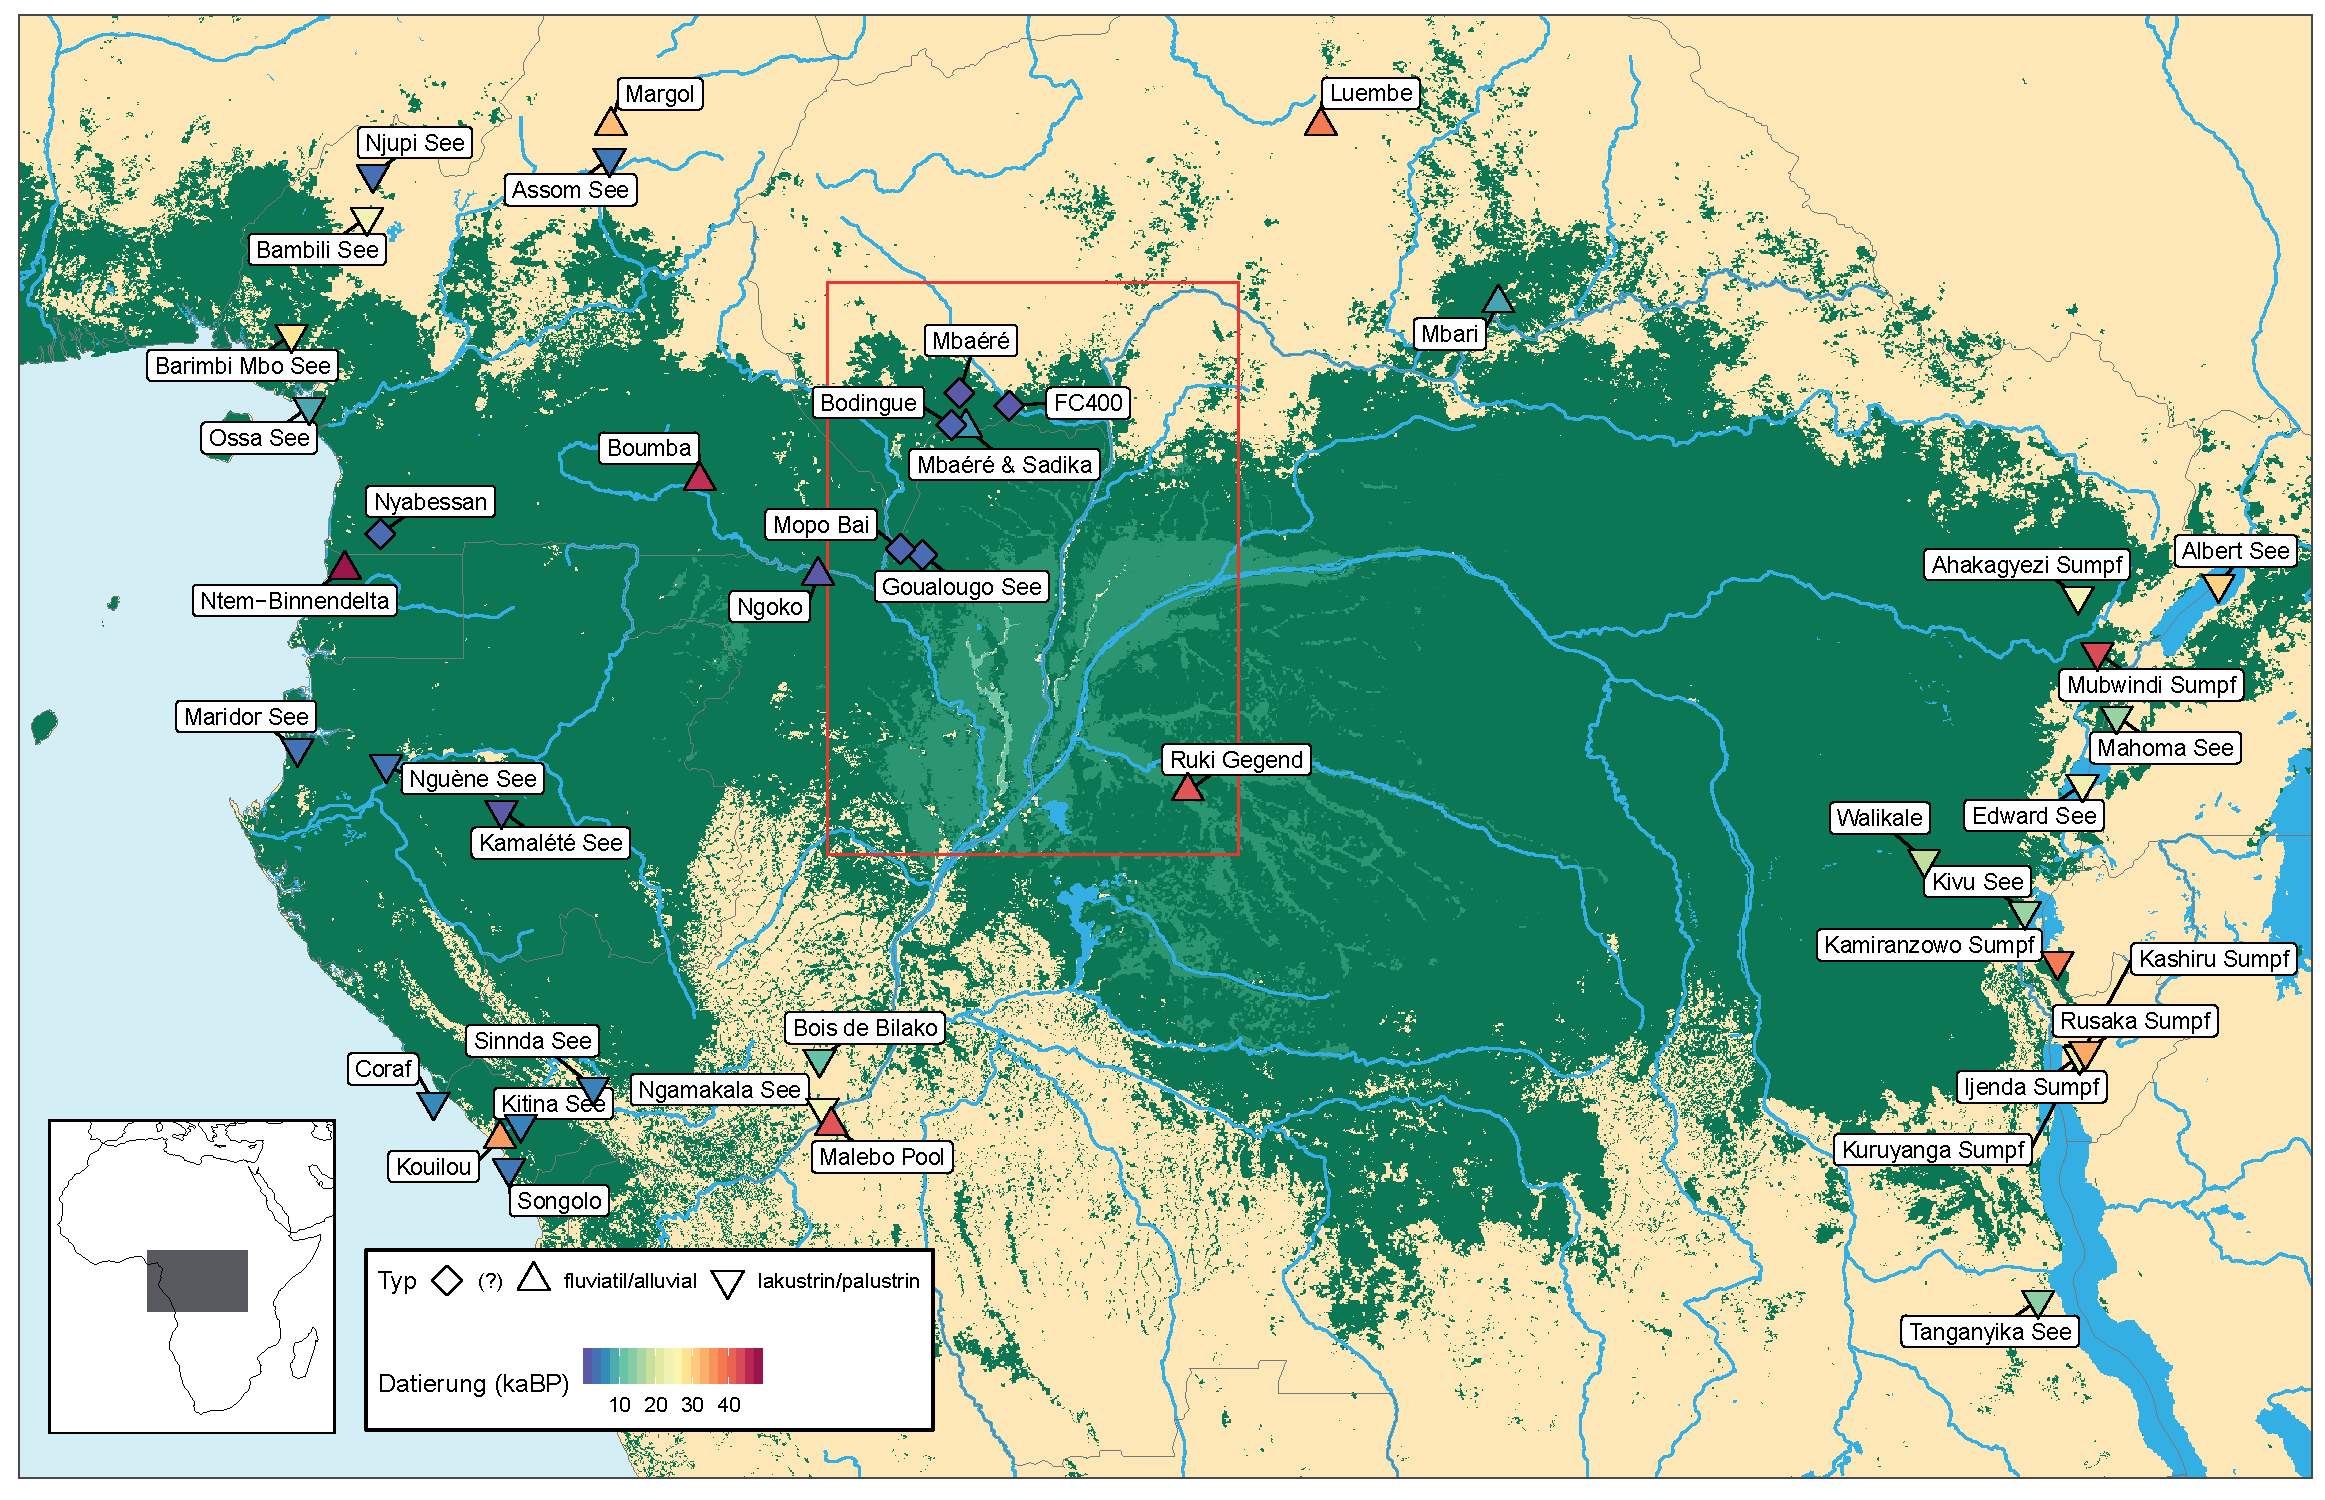
\includegraphics[width=\textwidth]{fig/Ch1_Fig2_PalaoUmwelt.pdf}
	\caption{Paläo-Umweltarchive und Vegetation: Kartierung der wichtigsten lakustrinen und palustrinen sowie fluviatilen und alluvialen Paläo-Umweltarchive sowie das maximale Alter der Ablagerungen \parencites[nach][]{Brncic.2007}{Brncic.2009}[43 Abb.~16, 46 Abb.~17]{Sangen.2009}{Kiahtipes.2011}{Kiahtipes.2016}. Rezente Verbreitung des immergrünen tropischen Regenwaldes (dunkelgrün) sowie Sumpfwald (hellgrün) nach \textcite{Mayaux.2003}. Das Arbeitsgebiet ist in rot hervorgehoben (siehe Abb.~\ref{fig:ArbeitsgebietKarte}).}
	\label{fig:PalaeoumweltArch_Karte}
\end{figure*}

Die Sichtweise, dass der tropische ombriophile Regenwald ein statisches Landschaftselement sei, konnte durch neuere Forschungen revidiert werden \parencite[83]{Runge.2001}. Es zeigte sich, dass der komplette Regenwald innerhalb von 40--100 Jahren durch einen komplexen Prozess kreislauforientierter Biomasseumsätze abgebaut und erneuert werden kann. Der immergrüne Regenwald des Inneren Kongobeckens bildet sich ab etwa 1600\,mm mittleren Jahresniederschlags aus (ebd. 83). Während der Waldbestand auf den Grundgebirgs-Latosolen im Randbereich homogen ist, zeigten sich im saisonal überfluteten Zentrum des Kongobeckens stärker heterogene Arten-Zusammensetzungen (ebd. 83\,f.). Die tropischen Wälder müssen folglich als \enquote{entwicklungsgeschichtlich und vom Standort abhängige, differenzierte Ökosysteme} (ebd. 92) betrachtet werden.

Beruhend auf der rezenten Variabilität des Baumartenbestandes wurde von \textcite{Maley.2001} die Ausdehnung des westlichen zentralafrikanischen Regenwaldes im ersten vorchristlichen Jahrtausend rekonstruiert. Diese zeigt ein zum heutigen Stand deutlich reduziertes und auf sogenannte \enquote{Refugien} begrenztes Verbreitungsbild. Die Nordgrenze der von \textsc{Maley} (ebd. 7 Abb.~4) postulierten Regenwaldverbreitung im Bereich des Laufs des \mbox{Ubangi} lag mutmaßlich deutlich südlich von Bangui (Fpl.~215) im Bereich zwischen Imese (Fpl.~201) und Dongo (Fpl.~202). Durch die ebenfalls postulierte Unterbrechung der Regenwaldverbreitung im Gebiet des \mbox{Sangha}, dem sogenannten \enquote{\mbox{Sangha}-Korridor}\footnote{Der auch \enquote{\mbox{Sangha}-Intervall} genannte Bereich beschreibt eine Zone zwischen 14--18$^\circ$~O, in der auffällige Pflanzengemeinschaften beobachtet werden können, die nicht zu den heutigen klimatischen Rahmenbedingungen der Region passen \parencite{Gond.2013}. Zu diesen Auffälligkeiten zählen die Anwesenheit der senegalesischen Dattelpalme (\textit{Phoenix reclinata}), die nirgends sonst im Regenwald beobachtet werden kann. Andererseits fehlen in dieser Region auch einige, für den äquatorialen Regenwald weiter westlich wie östlich charakteristische Pflanzen \parencite[356\,f.]{Bostoen.2015}. Entsprechende Beobachtungen ließen bereits \textcite{Letouzey.1968} eine potenzielle Verbindung zwischen dem nördlichen und südlichen Savannengürtel postulieren.\label{ftn:SanghaIntervall}} \parencites[siehe][]{Russell.2014}{Bostoen.2015} soll sich eine Grenze der Regenwaldverbreitung südlöstlich von Ouesso (Fpl.~265) ergeben haben.

Im engeren Arbeitsgebiet kamen in den letzten Jahren einige Paläo-Umweltarchive hinzu \parencites[siehe][]{Brncic.2007}{Brncic.2009}{Kiahtipes.2011}{Kiahtipes.2016}. Archive sind auch aus Kamerun, Gabun und dem Mündungsgebiet des Kongo bekannt \parencite[siehe][41--58; Abb.~\ref{fig:PalaeoumweltArch_Karte}]{Sangen.2009}. Während es im westlichen Zentralafrika\footnote{Gemeint sind hier die Staatsgebiete von Kamerun und Gabun sowie der Bereich der Kongomündung.} sowie im östlichen Zentral- und in Ostafrika -- vornehmlich in der Region der großen ostafrikanischen Seen -- eine Vielzahl von lakustrinen und palustrinen Paläo-Umweltarchiven gibt, liegen aus dem Kongobecken keine entsprechenden Archive vor (ebd. 54 Abb.~16). Mit Blick auf die fluvialen und alluvialen Paläoumweltarchive sieht die Situation insofern besser aus, als hier die Arbeiten von Johannes \textcites{Preu.1986}{Preu.1986b}{Preu.1990} im Bereich des Ruki genannt werden können. Weitere Untersuchungen fanden am Rand des Kongobeckens in einem Talabschnitt des Mbaéré im Südwesten der Zentralafrikanischen Republik statt \parencite{Neumer.2007}.

Die Rekonstruktion extralokaler Einflüsse auf die Ökologie aus punktuellen Ergebnissen und regionalen Vergleichen bildet eine der grundlegenden Schwierigkeiten für physiogeografische und umweltgeschichtliche Untersuchungen \parencite[42]{Sangen.2009}.\footnote{Die jüngste Phase der Erforschung der Landschaftsgeschichte Zentralafrikas wird von modernen Fernerkundungsverfahren bestimmt \parencite[6]{Runge.2001}. Die grundsätzlich schlechten Erhaltungsbedingungen für Pollen in den für gewöhnlich groben und stark oxidierten meso- bis cenozoischen Ablagerungen des Kongobeckens erschweren palynologische Studien. Als Folge verschob sich der Fokus paläoklimatologischer Untersuchungen in den Bereich geochemischer Analysen und der Untersuchung der sub-marinen Ablagerungen des Kongo-Schwemmkegels \parencite[312]{Giresse.2005b}. Die Turbidit-Ablagerungen im Kongo-Canyon sind ein direktes Resultat der Suspensionsfracht des Kongo und repräsentieren dessen Schwankungen im Zusammenhang mit Faktoren wie Meeresspiegelschwankungen, Tektonik und Klimaveränderungen \parencite[2176]{Savoye.2009}.} Für den Gegenstand dieser Arbeit sind vornehmlich die Einflüsse des Ökosystems und dessen Veränderungen auf die menschliche Besiedlung des Kongobeckens von Bedeutung. Aus dem tropischen Afrika liegen insgesamt nur sehr wenige komplette, vom Ende der letzten Eiszeit bis in die Gegenwart reichende Pollenprofile vor \parencite[2682]{Lezine.2013}, so zum Beispiel das Profil aus dem Sacred Lake in Kenia \parencite[65--73; Beilage Fig.~15]{Coetzee.1967} sowie jenes aus dem Barombi-Mbo-See in Kamerun \parencite{Maley.1991}. Für das Pleistozän im Inneren Kongobecken liegen lediglich vorläufige Untersuchungsergebnisse aus Analysen durch Emile Roche vor, wonach Pollen aus der Ruki- und Momboyo-Region auf eine offene Savannen-Landschaft sowie nahe Marsch-Areale und Galleriewälder hinweisen würden \parencite[181]{Fiedler.1985}.\footnote{Für die Untersuchung wurden organisch reiche Sedimentschichten aus Imbonga am Momboyo \parencite[siehe][542\,f. Karte~1 Fpl.~43]{Wotzka.1995} sowie Bokuma-Isoko am Ruki (Fpl.~18) analysiert, welche zwischen 25\,000--15\,000 bp datieren \parencite[182]{Fiedler.1985}. Eine direkte Publikation dieser Daten liegt nicht vor.}

Eines der aussagekräftigsten Paläo-Umweltarchive, durch das eine Rekonstruktion der Klimaentwicklung der Großregion möglich wird, stammt aus dem knapp 2\,km großen, nahezu kreisrunden und 110\,m tiefen Vulkansee Barombi Mbo in Westkamerun \parencite[159--161]{Maley.1998b}.\footnote{Der in der Seemitte genommene, 23,5\,m lange Sedimentkern BM-6 enthielt Schichten, die zirka 27\,500 Jahre zurückreichen, wobei die untersten 1,5\,m des Kerns eine, vermutlich durch vulkanische Aktivität verursachte, gestörte Lagerung aufwiesen \parencite[6 Abb. 1]{Maley.2001}. Auch aufgrund der allgemeinen Schwierigkeiten einer \textsuperscript{14}C-Datierung in diesen Zeiträumen werden die ältesten ansprechbaren Schichten auf vor 24\,000 Jahren datiert. Die Daten zeigen im für diese Arbeit wichtigen 1.~Jt. v.~Chr. einen Rückgang der Regenwald-Flora beziehungsweise Baumpollen zugunsten von Savannen-Taxa  \parencites[6 Abb. 1]{Maley.2001}[56--58]{Maley.2003}.} Mit Blick auf die Erkenntnisse aus dem Barombi Mbo-Kern wurden von \textcite[357--360]{Schwartz.1992} erstmals Überlegungen zu den Zusammenhängen zwischen der Aufsiedlung des zentralafrikanischen Regenwaldes durch keramikproduzierende und sesshaftlebende Gruppen in der zweiten Hälfte des 1.~Jt. v.~Chr., der Ausbreitung der Eisenmetallurgie in den letzten Jahrhunderten vor der Zeitenwende sowie der heute unter den Begriffen \textit{First Millennium BC Crisis} \parencite[63]{Sangen.2009} beziehungsweise \enquote{Krise des Regenwaldes} \parencite{Neumann.2014} bekannten klimatischen sowie damit einhergehenden ökologischen Veränderung des Regenwaldes nach etwa 1000 v.~Chr. angestellt.

Die Veränderung der Regenwald-Vegetation im 1.~Jt. v.~Chr. lässt sich auch im Pollenprofil aus dem Nyabessan-Sumpf im Ntem-Binnendelta in Südkamerun nachvollziehen \parencite[316]{Ngomanda.2009}. So zeichnet sich gegen 500 v.~Chr. in den Daten ein deutlicher Wandel der Regenwaldflora ab. Das zirka 1,8\,m mächtige und vom 13./11. bis in das 5./3.~Jh. v.~Chr. datierende Profil zeigt für die zweite Hälfte des 1.~Jt. v.~Chr. einen Rückgang des Sekundärwaldes zugunsten eines Anstiegs von Primärwald-Taxa \parencite[ebd. 311 Abb.~3; ][58 Abb.~5]{Neumann.2012}.

Daten für die holozäne Klimageschichte des Arbeitsgebietes liegen aus dem südlichen Teil des \enquote{Nouabalé-Ndoki National Park}, in der nördlichen Republik Kongo vor \parencite{Brncic.2007}.\footnote{Ein etwa 68\,cm langer Sedimentkern aus dem Goualougo-See deckt die letzten 3300~Jahre ab (\textsc{Brncic, Willis} u.~a. 2007: 236--237 Abb.~59). Die Untersuchung ergab, dass sich überregionale klimatische Vorgänge kaum niedergeschlagen haben, da feuchte semi-immergrüne Waldtaxa durch die gesamte, durch den Kern abgedeckte Zeit hindurch konstant vorkamen (ebd. 240). Anzeichen für eine Savannen-Ausbreitung konnten nicht beobachtet werden. In den vergangenen 1000 Jahren mehren sich Anzeichen für anthropogene Feuer. Verschiedene Pioniertaxa wie \textit{E. guineensis}, \textit{Tetrorchidium} sp. und \textit{Erythrophleum} sp. zeigen trockenere Perioden an (ebd.). Das Vorkommen dieser Taxa ist fast ausschließlich auf das 1.~Jt. v.~Chr. beschränkt (ebd. 236 Fig.~5).} Der anthropogene Einfluss auf die Vegetation der Region innerhalb der letzten 3000~Jahre ist demnach größer als jener der auf klimatische Veränderungen zurückgeht. Ein zweiter Sedimentkern stammt aus Mopo Bai, einer saisonal überfluteten, sumpfigen Niederung etwa 28\,km westnordwestlich des Goualougo-Sees \parencite[80]{Brncic.2009}. Der 1\,m lange Kern deckt die letzten 2500~Jahre ab und die Pollensequenz zeigt deutliche Einflüsse klimatischer und anthropogener Faktoren auf die Ökologie (ebd. 86). Die Holzkohlekonzentration nimmt ab dem 11.~Jh. n.~Chr. in Form mehrerer, ansteigender Spitzenwerte zu (ebd. 85 Abb.~5) und der Anteil von \textit{Elaeïs guineensis} -- einer Pioniertaxa -- ist um die Zeitenwende am größten und nimmt ab dann stetig ab (ebd. 83 Abb.~4).

Aus dem Ngotto-Waldschutzgebiet im äußersten Südwesten der Zentralafrikanischen Republik ist die Untersuchung von zwei Pollenkernen bekannt \parencite{Kiahtipes.2011}. Ein Sedimentkern wurde 2007 aus der Flussmarsch des Bodingue gezogen.\footnote{Der insgesamt 72\,cm lange Kern wurde in Abständen von 10\,cm beprobt. Drei aus dem oberen, mittleren und unteren Bereich des Kerns genommene \textsuperscript{14}C-Proben zeigen an, dass er eine Zeitspanne vom 5.~Jh. v.~Chr. bis zum 13.~Jh. n.~Chr. abdeckt (\textsc{Kiahtipes} u.~a. 2011: 4 Tab.~1; 5 Fig.~2).} Ein zweiter Kern stammt aus der Uferzone der Flussmarsch des Mbaéré.\footnote{Der 2,5\,m lange Kern wurde in Intervallen von 5\,cm beprobt. In die Analyse ging nur jede zweite Probe ein. Der Kern deckt eine Zeitspanne vom 7./8.~Jh. n.~Chr. bis in die Gegenwart ab (\textsc{Kiahtipes} u.~a. 2011: 11 Fig.~6).} Kombiniert bietet sich durch beide Kerne ein Einblick in die regionale Entwicklung für die letzten etwa 2500 Jahre (ebd. 4 Tab.~1, 5 Fig.~2). Nahe des Zusammenflusses der Flüsse Loame und Lobaye wurde in einer Region mit Feuchtsavannen-Vegetation ein 2\,m langer Sedimentkern erbohrt \parencite[5]{Lupo.2015}. Radiokohlenstoffdatierungen zeigten, dass der Kern Paläo-Umweltdaten der letzten 500 Jahre abdeckt (ebd. 13 Abb.~6). In der Auswertung zeigte sich ein Wechsel von einer dichten Regenwaldvegetation zu einer offeneren, savannenartigeren Vegetation im späten 17. oder frühen 18.~Jh.
\end{multicols}
\chapter{Quellen und Methoden}\label{sec:Quellen}
\begin{multicols}{2}
\raggedcolumns
\noindent Das im Rahmen dieser Arbeit bearbeitete Quellenmaterial umfasst 10\,519 Fundstücke von 122 individuellen Fundplätzen in einem 500\,$\times$\,700\,km großen Arbeitsgebiet (Kap.~\ref{sec:Arbeitsgebiet}). Das Material stammt zu einem großen Teil aus 143 individuellen Oberflächenabsammlungen.\footnote{Während an allen Fundstellen mindestens die moderne Dorffläche nach Funden wie Befunden abgesucht wurde, existieren von einigen Plätzen Komplexe aus zusätzlichen, spezifischen Bereichen (siehe Katalog B).} Eine belastbare Quellenbasis bildeten 13 ausgegrabene sowie sechs weitere, zwar als Befunde erkannte, aber nicht systematisch untersuchte Komplexe (Tab.~\ref{TabBefundeUntersucht}). Da keine exakten geografischen Koordinaten der Fundstellen bekannt waren, mussten diese nachträglich ermittelt werden.\footnote{Die Fundstellen wurden während der Befahrung der Flüsse in Flussatlanten, welche von der staatlichen, damals za{\"i}rischen Transport- und Schifffahrtsbehörde ONATRA (\textit{Office national des Transports}) stammten, verzeichnet. Die Erhebung der Koordinaten erfolgte durch Abgleich dieser um entsprechende Notizen ergänzten Flussatlanten mit GoogleEarth-Satellitendaten. Diese Vorgehensweise bedingt eine gewisse Unschärfe der ermittelten Positionen, da es von Fall zu Fall kleinere Unterschiede im Kartenmaterial gab. Die Positionen der Fundstellen innerhalb der Ortschaften ließ sich regelhaft nicht mehr präzise rekonstruieren. Die in GoogleEarth ermittelten Koordinaten für die Fundstellen wurden in Dezimalgrade umgerechnet und als Längen- sowie Breitenangabe aufgenommen (Anlage 1.B).} Die Vergabe von Katalognummern, im weiteren als \enquote{Fpl.} abgekürzt, schließt an den 185 Fundstellen umfassenden Katalog von \textcite[542\,f. Karte 1]{Wotzka.1995} an.

Die Aktenlage umfasste neben der ursprünglichen Dokumentation\footnote{Aufgrund des zeitlichen Abstandes zwischen den Feldarbeiten des \textit{River Reconnaissance Project} in den 1980er Jahren und der aktuellen Aufarbeitung konnten offene Fragen an die ursprüngliche Dokumentation nicht immer zufriedenstellend geklärt werden. Als zentrales Problem erwies sich das Fehlen der schriftlichen Felddokumentation von Célestin Kanimba Misago, dem damaligen Mitarbeiter der \textit{Musées Nationaux du Zaïre} (heute \textit{Institut des Musées Nationaux du Congo}) in Kinshasa und Kooperationspartner. Während die Feldbücher der übrigen Teilnehmer der Reisen von 1985 und 1987 im Original wie in Kopie vorlagen, konnten jene von Kanimba Misago nicht aufgefunden werden. Während der Kampagne von 1987 hatte Kanimba Misago die Komplexe BBS~87/1 (Kat.-Nr.~6) in Bobusa am unteren \mbox{Sangha} (Fpl.~239) und PIK~87/3 (Kat.-Nr.~10) in Pikunda am mittleren \mbox{Sangha} (Fpl.~255) ausgegraben. Der Metallurgie-Befund PIK~87/3, welcher nach Ausweis der vorliegenden Radiokohlenstoffdatierung in das 11.--13.~Jh. n.~Chr. (Abb.~\ref{fig:PIK87_Datierungen}) datiert und damit einer der ältesten Belege für einen flachen, offenen Ofen mit Schlackeabfluss in der Region darstellt, konnte ausschließlich auf einer nur bedingt systematischen fotografischen Dokumentation sowie einer Kurzbeschreibung durch \textsc{Kanimba Misago} aus dem Jahr 1995 beschrieben werden (Details siehe Kat.-Nr.~10), was bei der Bedeutung des Befundes bedauerlich ist.}, die im Gelände angefertigt wurde, auch eine Reihe von internen Berichten und Teile unveröffentlichter Manuskripte. Wo diese für die Aufarbeitung des Materials herangezogen wurden, sind sie entsprechend als Quelle im Text ausgewiesen. Die in dieser Arbeit durchgeführten Analysen gründen sich in allen Fällen auf den eigenen Beobachtungen des Autors am Fundmaterial sowie der Auswertung der im Gelände angefertigten Dokumentation (Katalog~A).

\section{Surveys, Grabungen und Befunde}\label{sec:GrabungenBefunde}

\subsection{Grubenbefunde}

In die Auswertung flossen 13 Grabungsbefunde von fünf verschiedenen Fundstellen ein sowie sechs Komplexe, die zwar einen klaren Befundcharakter aufweisen, aber nicht systematisch ergraben wurden (Tab.~\ref{TabBefundeUntersucht}, Katalog A). Zu letzterer Gruppe werden zum Beispiel die Komplexe MLB~85/103 (Kat.-Nr.~5) und LKW~87/186 (Kat.-Nr.~19) gerechnet, die zwar eindeutig als Gruben angesprochen werden können, jedoch nicht ausgegraben wurden. Da sich diese Beobachtungen aber aufgrund ihrer Geschlossenheit grundsätzlich von den ebenfalls in die Gesamtauswertung eingeflossenen Surveyfunden (Katalog B) unterscheiden, werden sie gemeinsam mit den Grabungsbefunde besprochen.

\begin{table*}[!t]
\centering
%\resizebox{\textwidth}{!}{%
{\footnotesize
\begin{sftabular}{@{}lllll@{}}
\toprule
\textbf{Fundstelle} & \textbf{Gruben} & \begin{tabular}[c]{@{}l@{}}\textbf{Metallurgie-}\\ \textbf{befunde} \end{tabular} & \textbf{Gräber} & \begin{tabular}[c]{@{}l@{}}\textbf{Schichten-}\\ \textbf{Abfolge} \end{tabular} \\
\midrule
\begin{tabular}[c]{@{}l@{}}\textbf{Maluba}\\(Fpl.~230)\end{tabular} & \begin{tabular}[c]{@{}l@{}}MLB 85/1-3-1\\ MLB 85/1-3-2\\ (MLB 85/2)\\ (MLB 85/103)\end{tabular} & & MLB 85/1-4-3 & \\ %\hdashline
\begin{tabular}[c]{@{}l@{}}\textbf{Bobusa}\\(Fpl.~239)\end{tabular} & & & & \begin{tabular}[c]{@{}l@{}}BBS 87/1\\ BBS 87/2\end{tabular} \\[3ex] %\hdashline
\begin{tabular}[c]{@{}l@{}}\textbf{Pikunda}\\(Fpl.~255)\end{tabular} & \begin{tabular}[c]{@{}l@{}}PIK~87/1\\ PIK~87/2\end{tabular} & PIK~87/3 & & \\[3ex] %\hdashline
\begin{tabular}[c]{@{}l@{}}\textbf{Ngombe}\\(Fpl.~252)\end{tabular} & (NGO~87/102) & & & \\[3ex] %\hdashline
\begin{tabular}[c]{@{}l@{}}\textbf{Mitula}\\(Fpl.~251)\end{tabular} & (MIT~87/103) & & & \\[3ex] %\hdashline
\begin{tabular}[c]{@{}l@{}}\textbf{Mobaka}\\(Fpl.~246)\end{tabular} & (MKA~87/102) & & & \\[3ex] %\hdashline
\begin{tabular}[c]{@{}l@{}}\textbf{Boleko}\\(Fpl.~285)\end{tabular} & & & BLK 87/1 & \\[3ex] %\hdashline
\begin{tabular}[c]{@{}l@{}}\textbf{Likwala Fluss-}\\ \textbf{Kilometer~186}\\(Fpl.~291)\end{tabular} & (LKW~87/186-1) & & & \\[3ex] %\hdashline
\begin{tabular}[c]{@{}l@{}}\textbf{Munda}\\(Fpl.~304)\end{tabular} & \begin{tabular}[c]{@{}l@{}}MUN~87/2-1-1 A \\ MUN~87/2-1-3\end{tabular} & \begin{tabular}[c]{@{}l@{}}MUN~87/1 \\ MUN~87/2-1-1 B/C \\ MUN~87/3\end{tabular} & & \\
\bottomrule
\end{sftabular}}
%}
\caption{Ausgegrabene Befunde: Übersicht über die untersuchten Befunde im Arbeitsgebiet aufgeteilt nach Befundkategorien. Die in Klammern stehenden Komplexe wurden nicht systematisch ausgegraben, aber als Befunde erkannt. Die Sortierung der Liste orientiert sich an der Abfolge, in der die Befunde untersucht wurden.}
\label{TabBefundeUntersucht}
\end{table*}

Im Jahr 1985 wurden bei der Befahrung der Flüsse \mbox{Ubangi} und Lua lediglich in Maluba am Lua (Fpl.~230, Kat.-Nr.~1--5) Grabungen durchgeführt. Von den insgesamt vier dort beobachteten Gruben wurden nur zwei vollständig untersucht und dokumentiert (Kat.-Nr.~1--2). Die ursprüngliche Verfüllung einer weiteren Grube (Kat.-Nr.~4) stürzte während der Grabung ein. Daher wurde der Befund nicht mehr weiter untersucht. Es wurden auch keine Funde dieses Befundes geborgen beziehungsweise zur Auswertung lagen keine Funde aus dieser Grube mehr vor. Eine vierte Grube (Kat.-Nr.~5) ist zwar als solche zu erkennen gewesen, es wurde aber lediglich eine geringe Menge keramischen Fundgutes entnommen und keine Grabung durchgeführt. Während der Kampagne von 1987 im nördlichen Teil der Republik Kongo, entlang der Flüsse \mbox{Sangha}, \mbox{Ngoko} und Liwkala-aux-Herbes sowie eines kurzen Abschnitts des Kongo, wurden zehn Befunde an vier verschiedenen Fundstellen untersucht. In Pikunda am mittleren \mbox{Sangha} (Fpl.~255) wurden an zwei benachbarten Grabungsstellen insgesamt drei Gruben (Kat.-Nr.~8--9) erfasst. In Munda am \mbox{Likwala}-\mbox{aux}-\mbox{Herbes} (Fpl.~304) fanden die umfangreichsten Ausgrabungen des \textit{River Reconnaissance Project} im Arbeitsgebiet statt. Innerhalb eines eng begrenzten Areals wurden vier Komplexe näher untersucht, die drei Gruben sowie drei Verhüttungsbefunde erbrachten. Die Grabungen MUN~87/1 (Kat.-Nr.~15) sowie MUN~87/2--1--1 (Kat.-Nr.~16) ergaben jeweils eine Grube sowie einen Verhüttungsbefund, während es sich bei Befund MUN~87/2--1--3 (Kat.-Nr.~17) um eine weitere Grube handelt.

Für das \mbox{Sangha}- und Likwala-aux-Herbes-Gebiet lassen sich auf Basis der ausgegrabenen Befunde in Pikunda (Fpl.~255) und Munda (Fpl.~304) Grundlagen der chronologischen Sequenz erarbeiten (siehe Kap.~\ref{sec:SequenzLikwala}--\ref{sec:SequenzSanghaNgoko}). Die Grabungen in Maluba am Lua (Fpl.~230) decken nur eine der belegten keramischen Stilgruppen ab und ermöglichen kaum weiterführende Aussagen zum Ablauf der Besiedlung im \mbox{Ubangi}- und Lua-Gebiet. Zwar liefern die Funde aus ausgegrabenen Kontexten oder eindeutig ansprechbaren Befunden die beste Datenlage, jedoch spiegeln sie nur sehr begrenzte Nutzungsphasen innerhalb der jeweiligen Fundstelle wider.

In Zentralafrika sind Grundbefunde die am häufigsten dokumentierte Befundkategorie und auch im Arbeitsgebiet wurden vor allem Gruben untersucht. Die Frage nach der Bedeutung dieser Befunde -- ihre Nutzung und Funktion in der Vergangenheit -- ist Gegenstand einer anhaltenden Diskussion \parencite[siehe][197--199]{Meister.2008b}. Während Merkmale wie die häufig in den Befunden beobachtete fragmentierte Gefäßkeramik sowie botanische Reste vordergründig eine profane Nutzung nahelegen, deuten andere Eigenschaften andere Verwendungen an. Der bislang ambitionierteste Interpretationsansatz stammt von \textcite{Wotzka.1993} und gründet auf die Feldarbeit des \textit{River Reconnaissance Project} sowie einem detaillierten Survey ethnologischer Literaturbelege. Die von Wotzka bearbeiteten 34 Grubenbefunde des Inneren Kongobeckens und die dabei beobachteten Deponierungen von Gefäßkeramik in ihnen bildeten die Grundlage für seine Auseinandersetzung mit der Frage nach der Funktion von Keramikdeponierungen in Gruben im zentralafrikanischen Regenwald. \textsc{Wotzka} (ebd. 262\,f. Tab.~1) stellte die an den Grubenbefunden beobachteten Merkmale zusammen und beschrieb sie im Sinne einer polythetischen, sich aus überschneidenden Typen zusammensetzenden Gruppe \parencite[siehe][37\,f. mit Abb.~3]{Clark.1968}. Aus archäologischer Perspektive kann er deutlich machen, dass es sich bei den von ihm untersuchten Befunden nicht um reine \mbox{Abfall-,} Vorrats-, Lehm- oder Lateritentnahmegruben handelt \parencite[264]{Wotzka.1993}. In der von ihm gesichteten ethnographischen Literatur berücksichtigte er auch an Gefäßkeramik aus Gruben beobachtbare Modifikationen oder intentionellen Zerstörungen von Böden oder Appliken (ebd.~262\,f. Tab.~1 Merkmale 6, 13 und 15). In seiner abschließenden Bewertung steht für \textsc{Wotzka} (ebd. 272) die \enquote{Erkenntnis, dass es zahlreiche in rezenter und subrezenter Zeit beobachtete Belege für rituelle Zerstörung von Keramik und anderen Sachgütern gibt, die in einem allgemeinem Zusammenhang mit dem Totenkult stehen}.\footnote{Erste geochemische Untersuchungen von Grubensedimenten aus Fundstellen in Südkamerun offenbarten eine Anreicherung von Phosphat im Bereich der Grubensohlen \parencites[722--724]{MbidaMindzie.19951996}{MbidaMindzie.1998}[147--150; 151--155]{Eggert.2016}. Während \textcite[209]{MbidaMindzie.1998} die auffällige Phosphatanreicherung, die in drei Gruben der Fundstelle Nkang beobachtet wurde, mit anthropogenen Faktoren in Verbindung bringt, weisen \textcite[151--155]{Eggert.2016} auf die Nichtberücksichtigung einer durch die niedrigen ph-Werte möglichen natürlichen Akkumulation hin. Im Zuge der vorliegenden Untersuchung wurde die Fragmentierung der in den Grubenbefunden des Arbeitsgebietes angetroffenen Gefäßkeramik dezidiert aufgenommen (siehe Abb.~\ref{fig:Fragmenierung_MLB85-131}, \ref{fig:Fragmenierung_MLB85-132}, \ref{fig:Fragmenierung_BBS87-1}, \ref{fig:Fragmenierung_BBS87-2}, \ref{fig:PIK87-1_Fragmentierung}, \ref{fig:BLK87-1_Keramik_Fragm}, \ref{fig:MUN87-1_Fragmentierung}, \ref{fig:MUN87-211_Fragmentierung}, \ref{fig:MUN87-213_Fragmentierung}). Während diese Verteilungen zwischen den verschiedenen Formen von Gruben und generell zwischen den Befundkategorien deutlich voneinander abwichen, steht eine spezifische Diskussion der daraus abzuleitenden Schlüsse noch aus.\label{ftn:GeochemieGruben}} Eine universelle Ansprache der Nutzung und Funktion von Gruben in Zentralafrika ergibt sich auch durch die Studie Wotzkas nicht, jedoch erweitert sie den Interpretationsansatz über allzu simple, profane Nutzungsmuster hinaus um eben jene sozialen Komponenten, die Gruben und vor allem die charakteristischen Deponierung von Gefäßkeramik als Teil des Alltags der prähistorischen Gesellschaften Zentralafrikas interpretierbar machen. Weiterhin muss jeder Befund individuell angesprochen und auf seine Genese hin untersucht werden.\footnote{Der Wandel von Nutzungsmustern über die Dauer des Bestehens eines Befundes lässt sich in geradezu exemplarischer Weise am Befund MUN~87/2-1-1 (Kat.-Nr.~16) in Munda am oberen \mbox{Likwala}-\mbox{aux}-\mbox{Herbes} (Fpl.~304) ablesen.}


\subsection{Sonstige Befunde}

Neben den Gruben zählen zu den archäologisch untersuchten Befunden im Arbeitsgebiet noch vier weitere Strukturen, die mit Eisenerzverhüttung in der Region in Zusammenhang gebracht werden können (Tab.~\ref{TabBefundeUntersucht}). Einer dieser Befunde wurde in Pikunda am \mbox{Sangha}, zusätzlich zu den genannten Gruben, als dritte Grabungsstelle erfasst (Kat.-Nr.~10). Die drei übrigen Befunde dieser Kategorie wurden ebenfalls 1987 bei den Ausgrabungen in Munda am \mbox{Likwala}-\mbox{aux}-\mbox{Herbes} untersucht. Neben den in den beiden Grabungsstellen MUN~87/1 (Kat.-Nr.~15) sowie MUN~87/2-1-1 (Kat.-Nr.~16) erfassten Verhüttungsstrukturen wurde in unmittelbarer Nähe ein weiterer Ofenbefund beobachtet und unter der Befundnummer MUN~87/3 (Kat.-Nr.~18) untersucht.

Zusätzlich zu den genannten Verhüttungsbefunden wurden zwei Bestattungen erfasst. Bei der Grabung im Jahr 1985 in Maluba am Lua (Fpl.~230) wurde zwischen den beiden ausgegrabenen Gruben (Kat.-Nr.~1--2) eine in einer kleinen Eingrabung angelegte Sekundärbestattung (Kat.-Nr.~3) erfasst und dokumentiert. Ein subrezentes Körpergrab (Kat.-Nr.~14) wurde 1987 in Boleko am \mbox{Likwala}-\mbox{aux}-\mbox{Herbes} (Fpl.~285) archäologisch untersucht.

Zwei zur Erfassung der jeweiligen Schichtabfolgen angelegte Sondageschnitte in Bobusa an der Mündung des \mbox{Sangha} (Fpl.~239) wurden ausgehend von bestehenden Bodeneingriffen angelegt. Sie waren jeweils nur 1\,m\textsuperscript{2} groß und reichten nur bis in etwa 1\,m Tiefe (Kat.-Nr.~6--7).


\subsection{Surveys}

Etwa zwei Drittel der untersuchten Funde stammen von Oberflächenabsammlungen. Zusammengenommen konnten 143 separate Komplexe von 118 Fundstellen herangezogen werden. Da die ausgegrabenen Befunde nur einen ungenügenden Einblick in die chronologischen Relationen zwischen den keramischen Stilgruppen boten und somit eine Rekonstruktion des Besiedlungsganges auf Basis dieser Daten nicht möglich war, musste dem von der Oberfläche der Dörfer abgesammelten Material verstärkt Beachtung geschenkt werden. Die Inventare aus Oberflächenabsammlungen setzen sich im Mittel aus jeweils gerade einmal 40 Fundstücken zusammen. Während die umfangreichsten Komplexe aus bis zu 289 Stücken bestehen, setzt sich die Hälfte aller Oberflächenabsammlungen aus weniger als 22 Fundobjekten zusammen. Neben den grundsätzlichen Schwierigkeiten im Umgang mit Funden aus Oberflächensurveys illustrieren die genannten statistischen Kennzahlen die Probleme bei der quantitativen Auswertung der entsprechenden Komplexe.

Die interne Zusammensetzung von Komplexen aus Oberflächensurveys ist grundsätzlich vielfältigen Parametern unterworfen.\footnote{Die Zusammensetzung eines Komplexes aus einem Oberflächensurvey ist nur zum Teil durch die archäologische sowie geomorphologische Situation an der Fundstelle bestimmt. In den hier zur Untersuchung vorliegenden Funden aus Dörfern im Zentralafrikanischen Regenwald ist aufgrund der gängigen Praxis des Fegens der Dorffläche zur Reinhaltung vor Bewuchs und Kleintieren mit einer großen Verlagerung von Objekten innerhalb der Fundstelle zu rechnen \parencite[355 Anm.~1]{Wotzka.1995}. Darüber hinaus spielen aber auch Faktoren eine Rolle, die mit dem Survey selbst zu tun haben, wie die Witterung, die Nutzung spezifischer Bereiche eines Dorfes zum Zeitpunkt des Surveys und auch die Erfahrung des Sammelnden.} Indizien für eine mögliche Vermischung von Funden ergaben sich im Zuge der Auswertung der Survey-Inventare von zwei im Gelände unterschiedenen Bereichen einer Fundstelle. Im Fall von zwei anderen Inventaren wurde eine Vermischung der Funde bereits 1990 festgestellt.\footnote{Aus Bobusa am unteren \mbox{Sangha} (Fpl.~239) liegen zwei direkt anpassende Scherben eines Reiseherdes vor (siehe Kap.~\ref{sec:Reiseherde}). Während ein Stück im Dorf (BBS~87/101:10) gefunden wurde, stammt eine weiteres, direkt anpassendes Fragment aus der als \textit{elali} (siehe Anm.~\ref{ftn:elali}) bezeichneten Dorfwüstung (BBS~87/102:81). Nach den Angaben im Feldbuch von Manfred Eggerts lag das \textit{elali} etwa 7 Weg-Minuten vom Dorf entfernt. Auf Basis der vorliegenden Unterlagen kann eine simple Verwechslung der Nummerierung bei der Beschriftung der Stücke im Anschluss an die Feldkampagne von 1987 nicht ausgeschlossen werden. Inwieweit eine mögliche Verlagerung der Funde auf natürlichem oder artifiziellem Wege bestehen kann, muss offenbleiben. Das Material des Komplexes NGO~87/101 aus Ngombe am \mbox{Sangha} (Fpl.~252) wurde zu einem nur grob eingrenzbaren Zeitpunkt mit jenem des Komplexes NGL~87/101 aus Ngombe am \mbox{Likwala}-\mbox{aux}-\mbox{Herbes} (Fpl.~283) vermischt. Allen Funden des Komplexes NGO~87/101 wurde die Kennung NGL~87/101 gegeben. Erkannt wurde dieser Umstand erst 1990 von Eggert, als ihm bei einer Durchsicht der Funde der Kampagne von 1987 auffiel, dass \textit{offiziell} keine Funde mit der Kennung NGO 87/101 vorliegen. Im Fall der Scherben aus den beiden Fundstellen muss die Vermischung bereits sehr zeitig, möglicherweise bereits im Feld, bei der Vorbereitung des Exports der Funde oder kurz danach stattgefunden haben. In den verfügbaren Packlisten waren bereits nur die beiden Komplexe NGL~87/101 und NGO~87/102 und kein Komplex NGO~87/101 verzeichnet. Ein entsprechender Komplex ist jedoch eindeutig im Feldbuch Eggerts sowie der Kartei der Fundstellenkürzel mit der Beschreibung \enquote{Dorf allgemein} ausgewiesen. Im Zuge der Aufarbeitung der Funde ergaben sich nur wenige stichhaltige Indizien, die eine Trennung des mit NGL~87/101 beschrifteten Materials, insgesamt 112 Scherben, auf zwei Komplexe ermöglichten. Auffällig ist das Auftreten von rouletteverzierter Keramik, die an Fundstellen entlang des Likwala-aux-Hebers kaum beobachtet wurde (siehe Kap.~\ref{sec:SequenzLikwala}), am \mbox{Sangha} jedoch durchaus vertreten ist (siehe Kap.~\ref{sec:SequenzSanghaNgoko}). Beruhend auf den Inventaren der jeweils benachbarten Fundstellen konnte unter Vorbehalten das jeweilige Ensemble der Stilgruppen an den beiden Fundplätzen rekonstruiert werden (siehe Tab.~\ref{tab:LikwalaSequenz}, \ref{tab:SanghaNgokoSequenz}).\label{ftn:Vermischungen}}

\section{Funde}

Die umfangreichste Fundgattung innerhalb des untersuchten Materials bildet die Gefäßkeramik (Tab.~\ref{tab:Funde_Uebersicht}). Die insgesamt 8469 Gefäßeinheiten und Scherben machen 80\,\% des gesamten Fundgutes aus. Unter den restlichen, nichtkeramischen Funden nehmen Metallurgieüberreste, vor allem Schlacken mit 1321 Stücken beziehungsweise knapp 40\,kg eine hervorzuhebende Stellung ein. Die weiteren Fundkategorien sind häufig nur durch wenige Stücke vertreten.

\begin{figure*}[tb]
\noindent\begin{minipage}[b]{\columnwidth}
	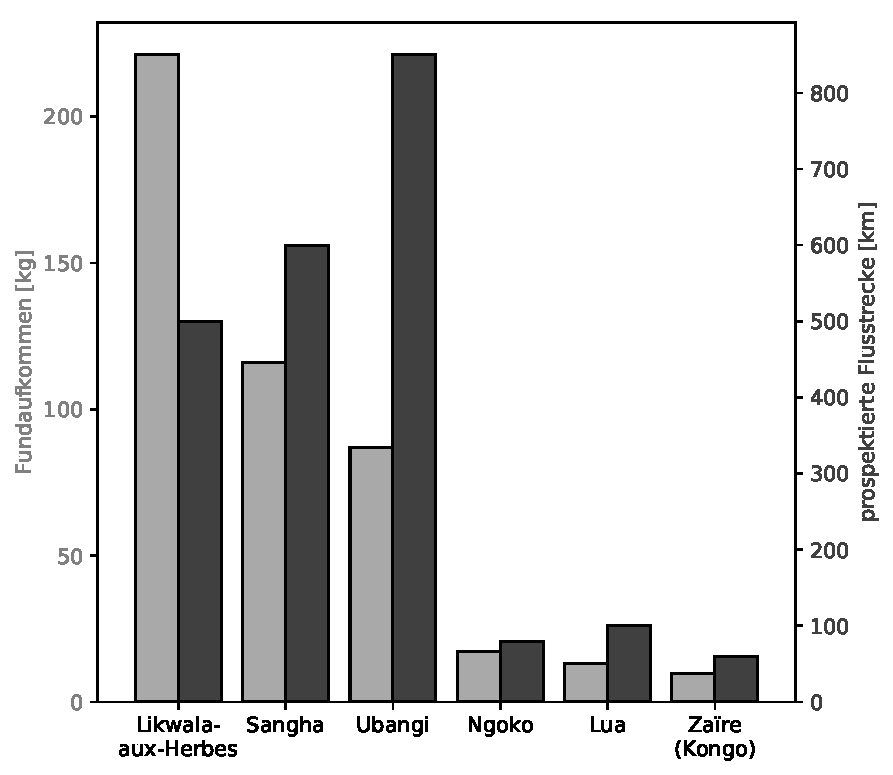
\includegraphics[width=\columnwidth]{fig/2-2_FundeGewicht_FlussKM.pdf}
	\captionof{figure}{Funde: Vergleich des Fundaufkommens (hell) mit Bezug auf die Länge des befahrenen Flussabschnitts (dunkel).\label{fig:FundGewVSFlussKM}}
\end{minipage}\hfill
\noindent\begin{minipage}[b]{\columnwidth}
{\footnotesize \begin{sftabular}{@{}p{.325\columnwidth}R{.125\columnwidth}R{.075\columnwidth}R{.175\columnwidth}R{.075\columnwidth}@{}}
		\toprule
		\textbf{Fundkategorie} &  \textbf{Anzahl} &     \textbf{\%} &  \textbf{Gew. (kg)} &     \textbf{\%} \\
		\midrule
		Gefäßkeramik &    8469 &   80,5 &        363,34 &   78,3 \\
		Schlacke &    1321 &   12,6 &         39,73 &    8,6 \\
		gebrannter Lehm &     187 &    1,8 &          6,25 &    1,3 \\
		Ofenwand &     182 &    1,7 &         19,88 &    4,3 \\
		keram. Sonderform &     117 &    1,1 &         11,19 &    2,4 \\
		Tuyere &      94 &    0,9 &          6,81 &    1,5 \\
		Stein &      76 &    0,7 &          7,23 &    1,6 \\
		Knochen &      29 &    0,3 &          5,93 &    1,3 \\
		Eisen &      13 &    0,1 &          0,53 &    0,1 \\
		Laterit &      11 &    0,1 &          0,08 &    0,0 \\
		Glas &       6 &    0,1 &          0,01 &    0,0 \\
		Metall &       8 &    0,1 &          0,38 &    0,1 \\
		Botanik &       2 &    0,1 &             - &      - \\ 
		Sonstige &       5 &    0,1 &          2,52 &    0,5 \\ \bottomrule			\multicolumn{1}{r}{\textbf{$\sum$}} &   10519 &  100 &        463,88 &  100 \\
		\bottomrule
	\end{sftabular}
}
\captionof{table}{Funde: Übersicht der in die Auswertung eingeflossenen Fundkategorien und ihrer Anteile.\label{tab:Funde_Uebersicht}}
\end{minipage}
\end{figure*}

Die Funde sind, obschon der Geländearbeit innerhalb beider Kampagnen die gleiche Surveystrategie zugrunde lag, nicht gleichmäßig im Arbeitsgebiet verteilt. Während einige Regionen sehr gut repräsentiert sind, liegen aus anderen Räumen nur vergleichsweise wenige Funde vor. Besonders deutlich wird dies bei einer Gegenüberstellung des Fundaufkommens von den drei größten, befahrenen Flüssen: \mbox{Ubangi}, \mbox{Sangha} und \mbox{Likwala}-\mbox{aux}-\mbox{Herbes} (Abb.~\ref{fig:FundGewVSFlussKM}). Die Funde vom \mbox{Ubangi}, der noch in der zweiten Hälfte der Feldkampagne von 1985 prospektiert wurde, machen weniger als 20\,\% des gesamten Fundmaterials aus, während die etwa 850\,km befahrene Strecke (Tab.~\ref{tab:ArbeitsgebietFlussstrecken}) knapp 40\,\% der in die Untersuchung eingeflossenen Flusskilometer entspricht. Die Prospektion entlang des \mbox{Ubangi} repräsentiert den längsten Transekt durch das Arbeitsgebiet, vom Zentrum des äquatorialen Regenwaldes nahe Mbandaka bis in die Savannenregionen nördlich von Bangui. Genau gegenteilig stellt sich das Verhältnis im Fall des \mbox{Likwala}-\mbox{aux}-\mbox{Herbes} dar (Abb.~\ref{fig:FundGewVSFlussKM}): das Fundmaterial von diesem Fluss steuert mit etwa 47\,\% knapp die Hälfte aller Funde bei, während die 500\,km lange Befahrung nur etwa 23\,\% der insgesamt befahrenen Flussabschnitte ausmacht. Der Anteil der Funde vom \mbox{Sangha} entspricht mit etwa 25\,\% dem Anteil der prospektierten Flussstrecke. Die Funde aus den befahrenen Gebieten entlang der Flüsse Lua, \mbox{Ngoko} und Kongo/Zaïre nehmen hingegen einen marginalen Anteil am Gesamtbestand ein. Allerdings gingen die Befahrungen dieser Flüsse nie über 100\,km hinaus (Tab.~\ref{tab:ArbeitsgebietFlussstrecken}) und von den jeweiligen Flüssen liegen lediglich zwischen vier und zehn Komplexen vor. Diese nehmen in der Analyse folglich nur eine nachrangige Stellung ein. In der Gesamtschau werden die Erkenntnisse, die sich aus der Befahrung des Lua ergaben, den Informationen vom \mbox{Ubangi} hinzugerechnet, da sich mit Blick auf die Besiedlungsgeschichte entlang des Lua keine eigenständige Entwicklung erkennen ließ (siehe Kap.~\ref{sec:SequenzUbangiLua}). In gleichem Maße werden die Untersuchungsergebnisse aus der Prospektion des \mbox{Ngoko} in direktem Zusammenhang zu den Erkenntnissen vom \mbox{Sangha} diskutiert (Kap.~\ref{sec:SequenzSanghaNgoko}).


\subsection{Gefäßkeramik}\label{sec:GefKeramik}

Die aus dem Arbeitsgebiet vorliegende Gefäßkeramik bildet den Grundstock der durchgeführten Analysen. Das Fundgut wurde mittels eines spezifischen Aufnahmesystems, welches sich vor allem an der Aufnahme von \textcite{Wotzka.1995} orientierte und um spezifische Elemente der Arbeiten von \textcites{Nordstrom.1972}{Stehli.1973}{Keding.1997}{Jesse.2003}{Clist.20042005} erweitert wurde, in einer relationalen Datenbank erfasst (siehe Kap.~\ref{sec:Datenhaltung}). Die Systematik der Aufnahme des für die Untersuchung wichtigen keramischen Fundmaterials gründet -- in Anlehnung an \textcite[57\,f.]{Stehli.1973} -- auf drei Aufnahme- und den sich daraus ergebenden Analyseebenen \parencite[siehe][36]{Keding.1997}:\footnote{Für die Ebenen 2 und 3 gilt die unten stehende Unterscheidung der Gefäßregionen (Abb.~\ref{fig:Keramik_VerzZonen}) in gleichem Maße.}
\begin{enumerate*}
	\item Technologie (Kap.~\ref{sec:Herstellung})
	\item Form (Kap.~\ref{sec:Keramiksequenz})
	\item Verzierung (Kap.~\ref{sec:Keramiksequenz})
\end{enumerate*}

%\vspace{\baselineskip}
\noindent Wann immer möglich wurden aus dem vorliegenden Scherbenmaterial Gefäßeinheiten -- im Folgenden GE genannt \parencite[siehe][81]{Jesse.2003} -- gebildet, die bei der Fundaufnahme im einzelnen beschrieben wurden. Die GE wurden, wenn sich keine direkten \textit{objektiven} Anpassungen ergaben, auf Basis eines \textit{subjektiven} Eindrucks der Zusammengehörigkeit gebildet (ebd.). Dieser Eindruck fußt auf einer Kombination von Formmerkmalen, Abmessungen beziehungsweise Dimensionierung und Verzierungen sowie den technologischen Eigenschaften, genauer dem \textit{Fabric}\footnote{Siehe \ref{sec:Herstellung2_Fabric}.} der Einzelstücke. Die Definition von GE ist für die statistische und chronologische Auswertung von Keramik unumgänglich, da ein Vorgehen auf Scherben-Niveau zu einer direkten Abhängigkeit beziehungsweise Korrelation der jeweiligen Analyseergebnisse vom Zerscherbtheitsgrad führen würde \parencites[siehe][36\,f.]{Keding.1997}[nach][483]{Drew.1988}.\footnote{Das keramische Fundgut des Inneren Kongobeckens wurde durch \textcite[38]{Wotzka.1995} in einem entsprechenden System aufgenommen. Eine individuelle Aufnahme umfasste alle auswertbaren Stücke. Scherben wurden zu Gefäßen zusammengefasst, wenn sich direkte Anpassungen oder eine hinreichende Übereinstimmung von Merkmalen ergab. Die Keramik aus den untersuchten Grabungsbefunden (ebd.~302--390 Kat.-Nr.~1--61) wurde um nicht aussagekräftige Stücke reduziert, während für die Fundinventare aus Oberflächensurveys nach dem Teilmengenprinzip aussortiert wurde (ebd.~38). Lediglich für einzelne Merkmalskombinationen repräsentative Stücke wurden aufgenommen.}

Das untersuchte keramische Material setzt sich fast ausschließlich aus Wandscherben (56\,\%) und Randscherben (40\,\%) zusammen. Ganze Gefäße (2\,\%) machen ebenso wie Bodenscherben (2\,\%) nur einen verschwindend kleinen Anteil am keramischen Inventar aus. Insgesamt 41\,\% aller Stücke können eindeutig einer keramischen Stilgruppe zugeordnet werden. Bei 25\,\% des Materials ist die Zuordnung fraglich, während 33\,\% des Materials keiner Stilgruppe zugewiesen werden kann und als unbestimmt gilt.

\begin{figure*}[!tb]
\centering
\begin{subfigure}{\columnwidth}
\centering
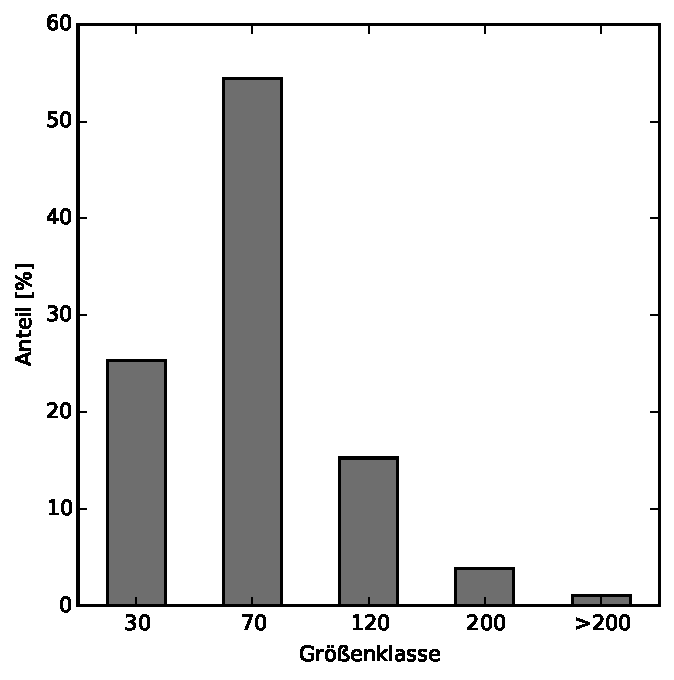
\includegraphics[height=.9\textwidth]{fig/2-2-1_KeramikFragmentierung.pdf}
\caption{Fragmentierung der Scherben (Größenklassen siehe Anm.~\ref{ftn:Keramik_Fragmentierung}).\newline}
\label{KeramikFragmentierung}
\end{subfigure}\hfill
\begin{subfigure}{\columnwidth}
\centering
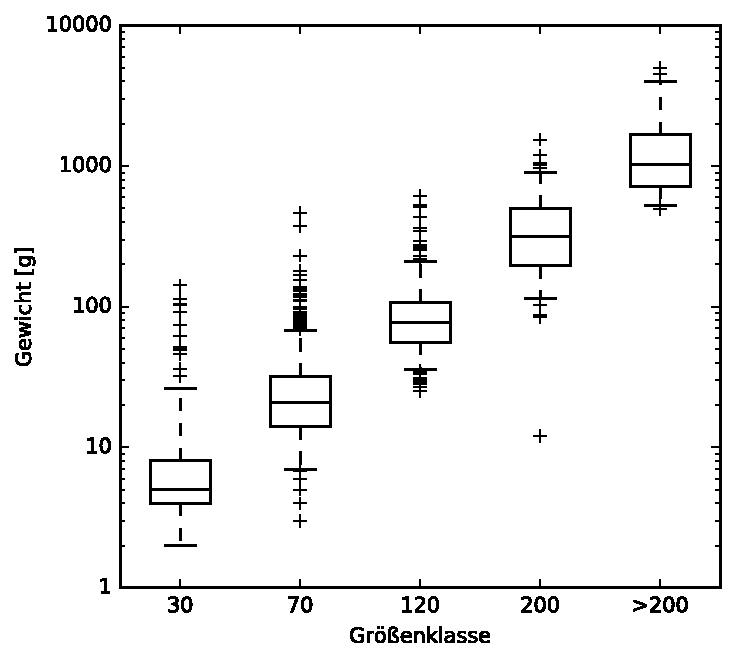
\includegraphics[height=.9\textwidth]{fig/2-2_Keramik_Gr-Gew_BoxPlt_2.pdf}
\caption{Verhältnis von Scherbengröße und Gewicht (Größenklassen siehe Anm.~\ref{ftn:Keramik_Fragmentierung}; 4218~GE).}
\label{fig:Keramik_FragmGrGew_B}
\end{subfigure}
\caption{Funde: Fragmentierung.}
\label{fig:Keramik_Typen-Fragm}
\end{figure*}

Der Anteil an unverzierten Stücken im Vergleich zu jenen GE aus dem untersuchten Materialkomplex, die Verzierungen aufweisen, variiert zwischen den Komplexen aus Oberflächensurveys und jenen aus Grabungen nur leicht. Während unverzierte Stücke in Oberflächenabsammlungen etwa 25\,\% ausmachen, sind es bei den ausgegrabenen Komplexen (Kat.-Nr.~1--19) knapp 29\,\%. Im Anschluss an die Ausgrabung der beiden Komplexe PIK~87/1 (Kat.-Nr.~8) sowie PIK~87/2 (Kat.-Nr.~9) in Pikunda am \mbox{Sangha} (Fpl.~255) wurde nachweislich unverziertes Scherbenmaterial verworfen. Im vorliegenden und ausgewerteten Fundmaterial dieser beiden Grabungen machen unverzierte Stücke immer noch 26\,\% aller GE aus. Daraus kann gefolgert werden, dass die Selektion der Stücke im Gelände die Repräsentanz des Fundinventares nur teilweise beeinträchtigt hat. Die Grabungen in Maluba am Lua (Fpl.~230; Kat.-Nr.~1--5), für die ein Aussondern \textit{nicht-diagnostischer} Stücke nicht überliefert ist, umfassten hingegen lediglich 18\,\% unverzierte Scherben. Diese Angaben legen nahe, dass die Oberflächenabsammlungen, zumindest mit Blick auf das Verhältnis von verzierten zu unverzierten Stücken, nicht grundsätzlich unrepräsentativ sind.


\subsubsection{Erhaltung}

Von den insgesamt 4217 aufgenommenen Gefäßeinheiten bestehen nur 654 aus mehr als einer Scherbe. Im Mittel bestehen die Gefäßeinheiten aus etwa 1,5 Scherben, was eine sehr starke Fragmentierung anzeigt und als Indikator für eine schlechte Erhaltung gewertet werden kann \parencite[siehe][86]{Jesse.2003}. Das mittlere Gewicht einer Gefäßeinheit liegt bei knapp 67\,g, das mittlere Gewicht der Einzelscherben bei rund 51\,g.\footnote{Der Unterschied ist wohl einzig auf die stark schiefen Verteilungen zurückzuführen.} Die Fragmentierurng der GE beziehungsweise der Zerscherbtheitsgrad der Keramik wurde unter Nutzung einer Größenklassen-Systematik aufgenommen, welche zuletzt auch bei \textcite[89]{Clist.20042005} zur Anwendung kam.\footnote{Die im Rahmen der Aufnahme genutzten Größenklassen beschreiben die Fragmentierung der Stücke mittels fünf fester Klassen (siehe \textsc{Clist}~2004/2005:~89): \textit{stark fragmentierte} beziehungsweise \textit{kleine Stücken} sind jeweils kleiner als 30\,$\times$\,30\,mm. Im ursprünglich auf \textcite[379]{Joukowsky.1980} zurückgehenden Schema liegt die kleinste Klassengrenze bei 25\,$\times$\,25\,mm \parencites[nach][]{Claes.1985}{deMaret.1985}[89]{Clist.20042005}. \textit{Mittelgroße} beziehungsweise \textit{mittelstark fragmentierte Stücke} sind zwischen  30\,$\times$\,30\,mm und 70\,$\times$\,70\,mm groß. Die nächste Klassengrenze liegt bei 120\,$\times$\,120\,mm und beschreibt \textit{gering fragmentierte} beziehungsweise \textit{große Stücke}. Stücke mit einer Größe zwischen 120\,$\times$\,120\,mm und 200\,$\times$\,200\,mm sind \textit{kaum fragmentiert} beziehungsweise \textit{groß}, während Objekte größer als 200\,$\times$\,200\,mm in der Regel große Gefäßfragmente oder ganze Gefäße widerspiegeln. Eine Dokumentation der erhalten Anteile von Gefäßprofilen und Randdurchmessern erfolgte nicht \parencite[siehe hierzu][155\,f.]{Claen.2011}. Die genannten Größenklassen wurden auch auf das nichtkeramische Fundgut, etwa Schlacken angewandt.\label{ftn:Keramik_Fragmentierung}} Während etwa 25\,\% der Keramik sehr stark fragmentiert sind -- kleiner als 30\,$\times$\,30\,mm -- sind knapp über die Hälfte der Scherben zwischen 30\,$\times$\,30\,mm und 70\,$\times$\,70\,mm groß (Abb.~\ref{KeramikFragmentierung}). Stücke größer als 70\,$\times$\,70\,mm sind seltener vertreten und machen zusammen nur etwa 20\,\% des Materials aus.


\begin{table*}[tb]
	\noindent\begin{minipage}[b]{\columnwidth}
		\centering
		{\footnotesize
			\begin{sftabular}{@{}llr@{}}
				\toprule
				\textbf{Schlüssel} & \textbf{Größenklasse} & \textbf{Durchmesser} \\
				\midrule
				VF & Very Fine & 62--125~$\mu$m \\
				F & Fine & 125--250~$\mu$m \\
				M & Medium & 250--500~$\mu$m \\
				C & Coarse & 500--1000~$\mu$m \\
				VC & Very Coarse & 1000--2000~$\mu$m \\
				\bottomrule
		\end{sftabular}}\vspace{1em}
		\captionof{table}{Keramik: Korngrößen nach der \textit{Wentworth-Grainsize-Scale}.\label{tab:Keramik_PartikelGr}}
	\end{minipage}\hfill
	\noindent\begin{minipage}[b]{\columnwidth}
		\centering
		{\footnotesize
			\begin{sftabular}{@{}lll@{}}
				\toprule
				\textbf{Schlüssel} & \textbf{Farbe} & \textbf{MUNSELL-Wert} \\
				\midrule
				S & schwarz/black & 10 YR 2/1 \\
				G & grau/grey & 10 YR 6/1 \\
				W & weiß/white & 10 YR 8/1 \\
				Bg & beige-ocker/yellow & 10 YR 8/6 \\
				Br & braun/dark reddish brown & 2.5 YR 3/4 \\
				R & rot/red & 2.5 YR 4/8--5/8 \\
				\bottomrule
		\end{sftabular}}
		\captionof{table}{Keramik: Farben der Scherbenoberflächen und -brüche.\label{tab:Keramik_Farbe}}
	\end{minipage}
\end{table*}

Die fünf Größenklassen bilden die Fragmentierung in einem zufriedenstellenden Maß ab, wie eine Gegenüberstellung mit den individuellen Scherbengewichten ergab (Abb.~\ref{fig:Keramik_FragmGrGew_B}). Trotz Ausreißern zeigen die Verteilungen, dass für jede der Größenklassen ein Gewichtsbereich angegeben werden kann, welcher sich von jenem einer anderen Größenklasse im Interquartilabstand unterscheidet. Überlappungen der Verteilungen stellen sich erst bei Betrachtung der zweifachen Standardabweichung ein.\footnote{Zur Interpretation von Box-Whisker-Plots siehe auch \textcite[81]{Hedderich.2016}. Im Fall von Abb.~\ref{fig:Keramik_FragmGrGew_B} markieren die Whiskers beziehungsweise Antennen die 2-Sigma-Standardabweichung der jeweiligen Verteilungen, während die Box das untere (25\,\%) sowie das obere Quartil (75\,\%) anzeigt und die zentrale Linie den Median markiert. Wird die einfache Standardabweichung zugrunde gelegt, lässt sich keine Überschneidung der Verteilungen beobachten.} Die Verteilungen zeigen insgesamt eine breite Streuung mit einigen Ausreißern, überlagern sich aber nur im Randbereich.


\subsubsection{Technologie}\label{sec:AufnahmeTechnologie}

Zusätzlich zu einer formalen Analyse, die sich auf morphologische Charakteristika wie Verzierung der Keramik stützt (siehe Kap.~\ref{sec:Keramiksequenz}), bildet eine tiefgreifende Auseinandersetzung mit technischen Parametern eines der Kernziele der Untersuchung. Hierfür grundlegend war die Einbeziehung von keramik-technischen Parametern in das Aufnahmesystem. Die untersuchten Kriterien gründen vornehmlich auf den Untersuchungen von \textcite{Nordstrom.1972} zu sudanesischer Keramik, welche wiederum Ausgangspunkt der neuen Studie von \textcite{Riemer.2011} zu Material aus der Dakhla-Oase in Ägypten waren, an der sich die hier vorgelegte Untersuchung orientiert. Für die Analyse der technologischen Eigenschaften der Gefäßkeramik wurde ein Katalog aus Aufnahmekriterien formuliert, welcher die folgenden Kenngrößen umfasst:
\begin{itemize*}
	\item nichtplastische Partikel
	\begin{itemize*}
		\item Größe (nach \textit{Wentworth-Grainsize-Scale})
		\item Dichte \parencites[32]{Kinne.2009}[nach][]{Hodgson.1976}
		\item Art
	\end{itemize*}
	\item Farbe des Scherben
	\begin{itemize*}
		\item Kernfarbe
		\item (Brennfarbe)
		\item Unterteilung des Scherbens in Oxidationszonen
		\item Ausbildung der Grenze zwischen Oxidationszonen
	\end{itemize*}
	\item Strukturierung der Oberfläche
\end{itemize*}

\begin{figure*}[!tb]
	\centering
	\resizebox{\textwidth}{!}{%
		{\footnotesize
\begin{sftabular}{@{}m{.02\textwidth} m{.02\textwidth} *7{>{\centering\arraybackslash}m{.1\textwidth}} m{.25\textwidth} @{}m{0pt}@{}@{}} 
 &  & \multicolumn{7}{c}{\textit{Variante}} &  &  \\
 &  & \textbf{1} & \textbf{2} & \textbf{3} & \textbf{4} & \textbf{5} & \textbf{6} & \textbf{7} & & \\
\multirow{10}{*}{\rotatebox[origin=c]{90}{\textit{Grundform} \hspace{9cm}}} & \textbf{A} & 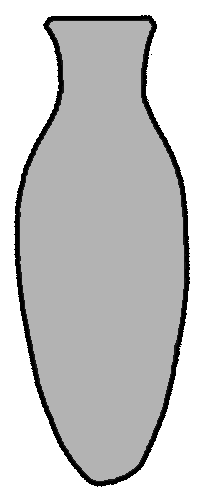
\includegraphics[height=.1\textwidth]{fig/Abb_GefFormen/G11c_Bolongo101.png} & 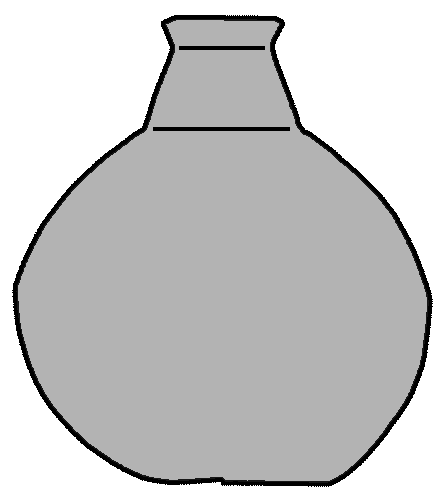
\includegraphics[height=.1\textwidth]{fig/Abb_GefFormen/G11b_MUN87-1-0-2-6-2.png} & 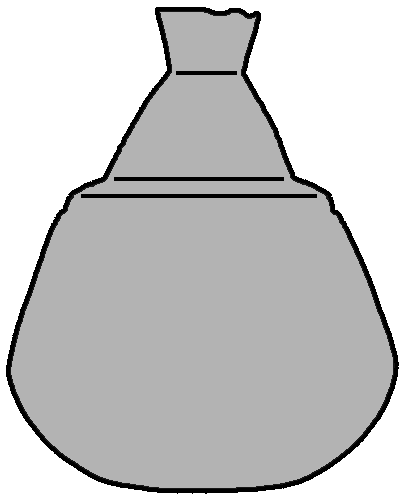
\includegraphics[height=.1\textwidth]{fig/Abb_GefFormen/G11a_MSG87-102-9a.png} &  &  &  &  & Flaschenförmige Gefäße & \\[.11\textwidth]
 & \textbf{B} & 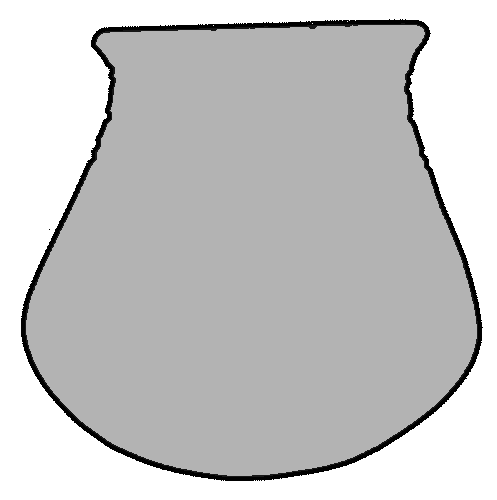
\includegraphics[height=.1\textwidth]{fig/Abb_GefFormen/G5_MUN87-2-1-3-8.png} & 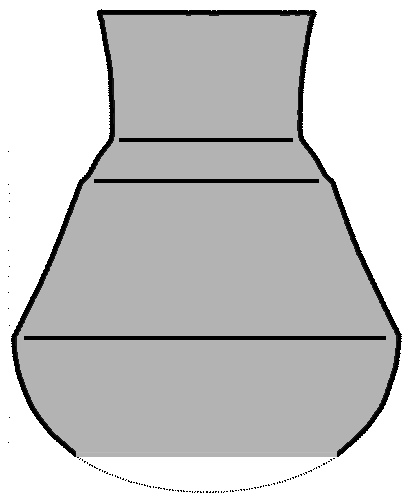
\includegraphics[height=.1\textwidth]{fig/Abb_GefFormen/G6c_msn87-101-145.png} & 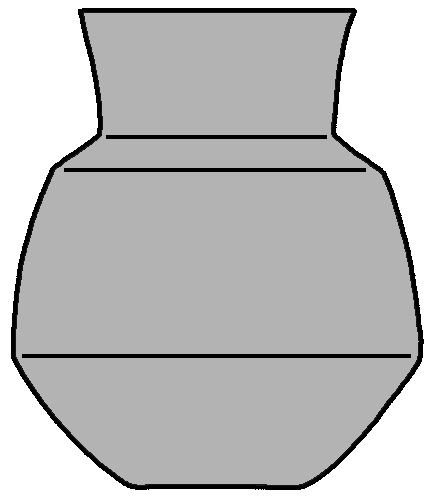
\includegraphics[height=.1\textwidth]{fig/Abb_GefFormen/G6b_ITN87-103-3a.png} & 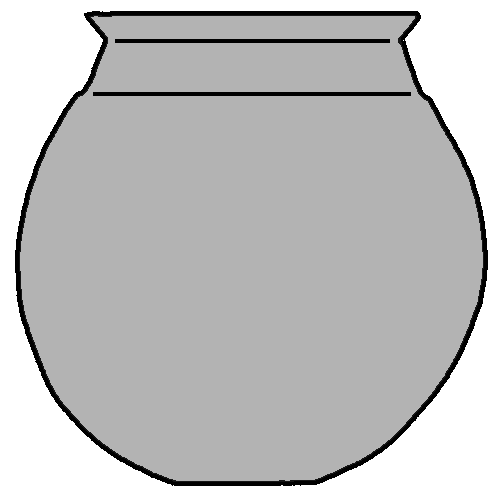
\includegraphics[height=.1\textwidth]{fig/Abb_GefFormen/G6a_MUN87-1-0-2-1.png} & 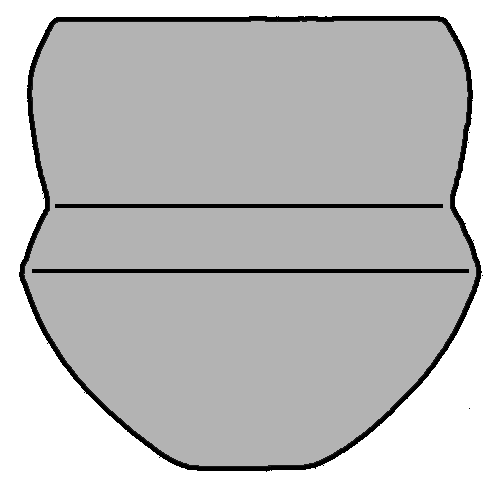
\includegraphics[height=.1\textwidth]{fig/Abb_GefFormen/G13_MKL85-101-114.png} & 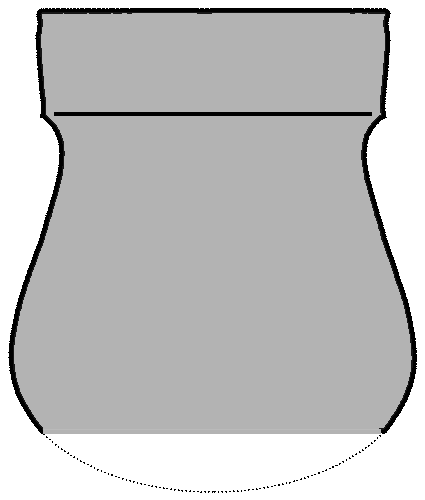
\includegraphics[height=.1\textwidth]{fig/Abb_GefFormen/G4_PIK87-101-51.png} & 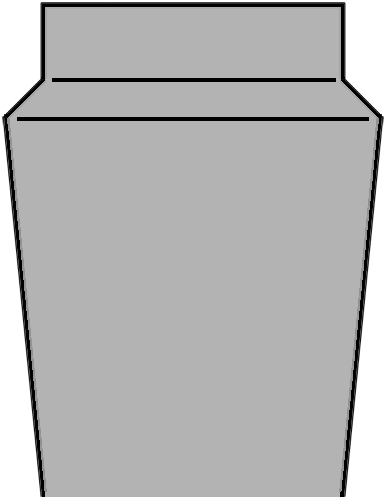
\includegraphics[height=.09\textwidth]{fig/Abb_GefFormen/G4b.png} & hohe Gefäße & \\[.11\textwidth]
 & \textbf{C} & 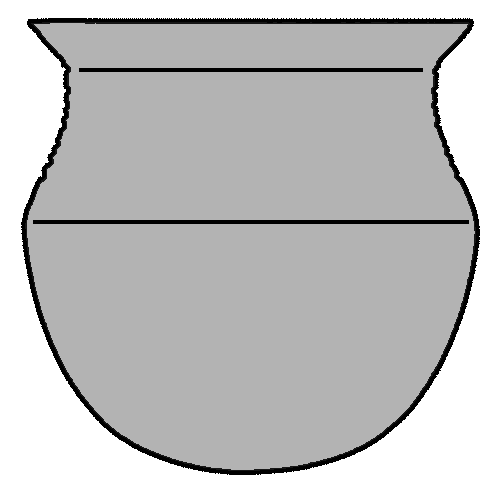
\includegraphics[height=.08\textwidth]{fig/Abb_GefFormen/G7a_NGB85-101-131.png} & 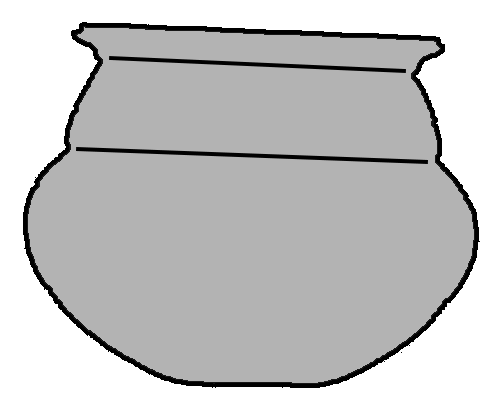
\includegraphics[width=.1\textwidth]{fig/Abb_GefFormen/G7b_DON85-102-a.png} &  &  &  &  &  & Gefäße mit leicht konvexer Wandung und ausgeprägtem Halsbereich & \\[.11\textwidth]
 & \textbf{D} & 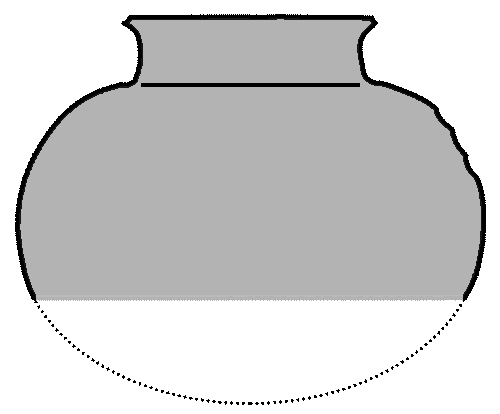
\includegraphics[width=.1\textwidth]{fig/Abb_GefFormen/G7c_PIK87-1-2-3_1-3-7.png} & 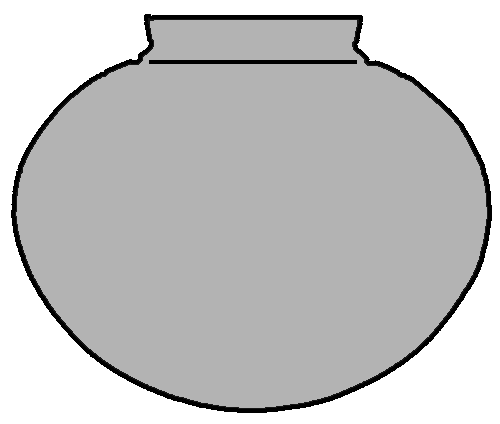
\includegraphics[width=.1\textwidth]{fig/Abb_GefFormen/G10a_NGO87-102-28-29.png} &  &  &  &  &  & Gefäße mit stark konvexer Wandung ohne ausgeprägten Halsbereich & \\[.11\textwidth]
 & \textbf{E} & 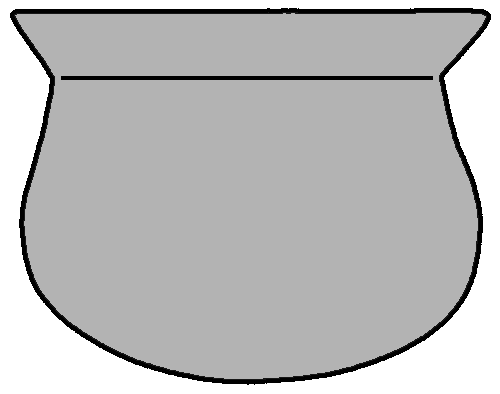
\includegraphics[width=.1\textwidth]{fig/Abb_GefFormen/G3_BLK87-1-1-1-2_HS.png} & 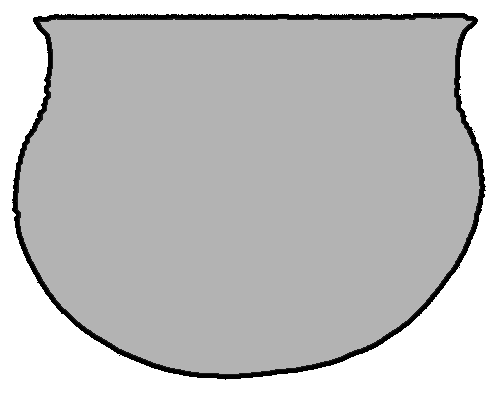
\includegraphics[width=.1\textwidth]{fig/Abb_GefFormen/G3c_MBN85-501-2.png} & 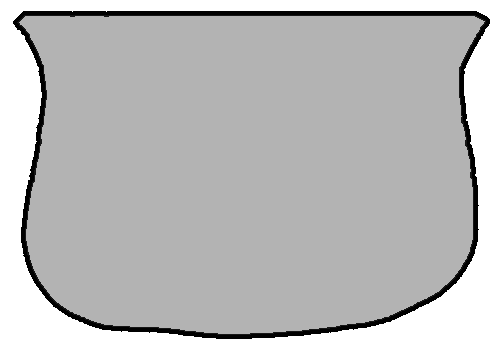
\includegraphics[width=.1\textwidth]{fig/Abb_GefFormen/G1b_MUN87-2-1-3.png} & 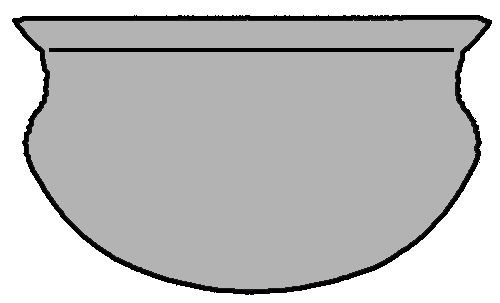
\includegraphics[width=.1\textwidth]{fig/Abb_GefFormen/G8b1_BLN85-201-b.png} & 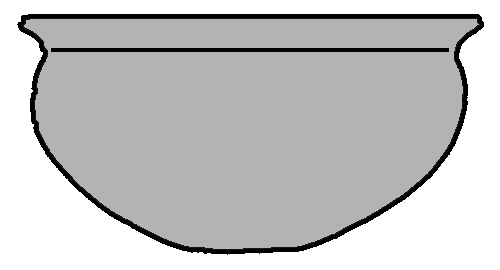
\includegraphics[width=.1\textwidth]{fig/Abb_GefFormen/G9b_DON85-102-b.png} & 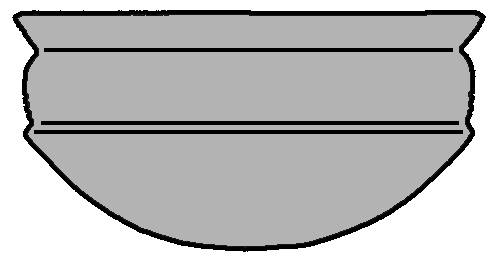
\includegraphics[width=.1\textwidth]{fig/Abb_GefFormen/G2d_SSL87-101-142.png} & 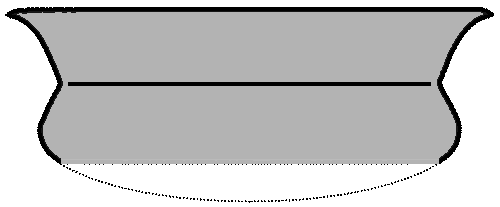
\includegraphics[width=.1\textwidth]{fig/Abb_GefFormen/G3b_GE5_BLK87-1-1-3-1-3.png} & Gefäße mit geschweifter Wandung & \\[.11\textwidth]
 & \textbf{F} & 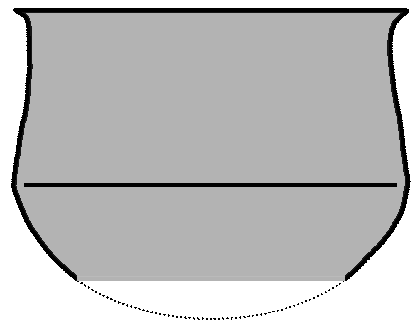
\includegraphics[width=.1\textwidth]{fig/Abb_GefFormen/G1c_LKW87-401-1.png} & 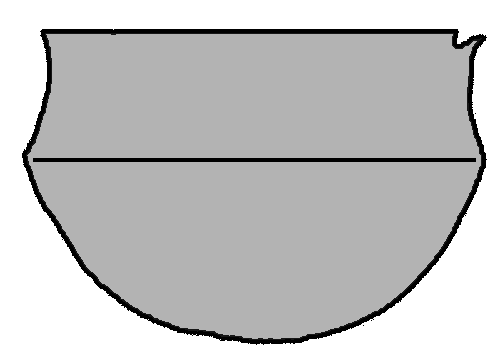
\includegraphics[width=.1\textwidth]{fig/Abb_GefFormen/G1d_MBJ_Roulettekeramik_E87-010-25.png} & 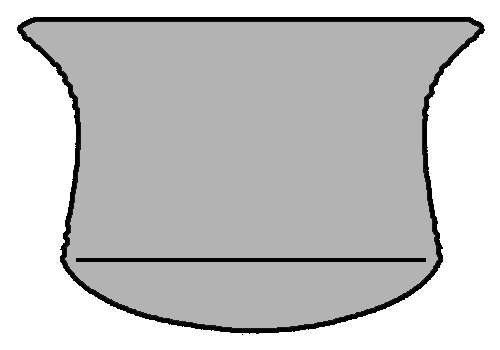
\includegraphics[width=.1\textwidth]{fig/Abb_GefFormen/G1a_PIK87-101-58.png} & 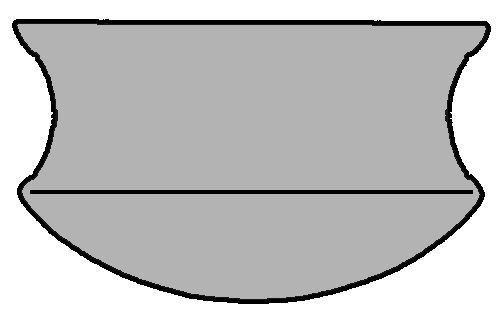
\includegraphics[width=.1\textwidth]{fig/Abb_GefFormen/G1a2_NGO87-102-27.png} & 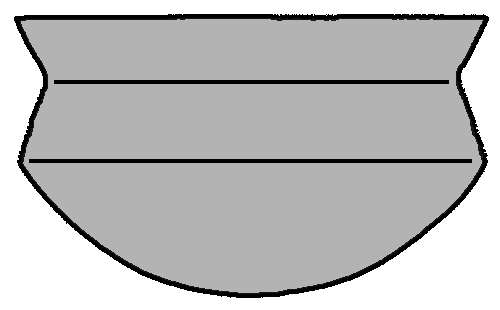
\includegraphics[width=.1\textwidth]{fig/Abb_GefFormen/G2e_INS87-102-2.png} & 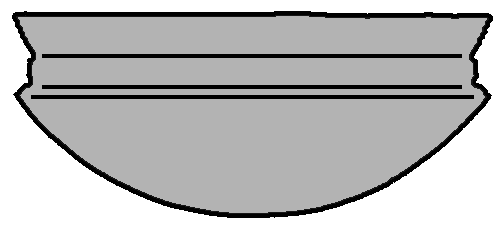
\includegraphics[width=.1\textwidth]{fig/Abb_GefFormen/G2a_NGO87-102-21.png} & 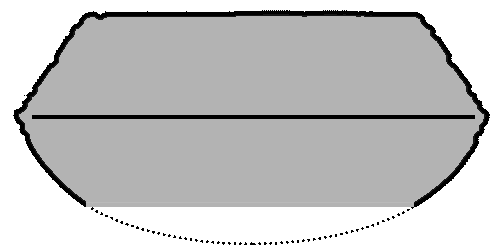
\includegraphics[width=.1\textwidth]{fig/Abb_GefFormen/G2h_MND85-101-33etc.png} & Gefäße mit abknickender Wandung & \\[.11\textwidth]
 & \textbf{G} & 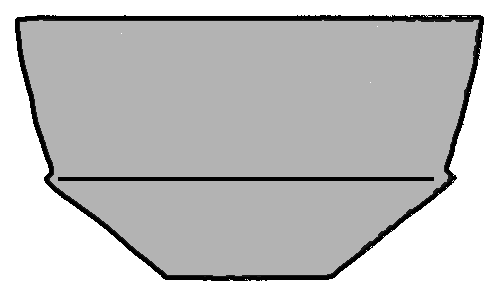
\includegraphics[width=.1\textwidth]{fig/Abb_GefFormen/G2b_ITN87-103-9.png} & 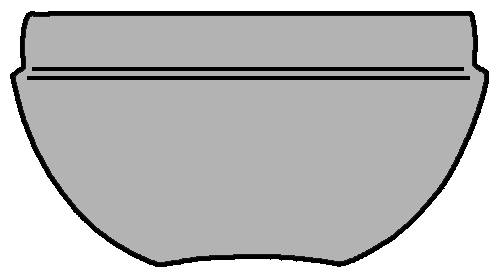
\includegraphics[width=.1\textwidth]{fig/Abb_GefFormen/G2c_MSG87-102-11.png} & 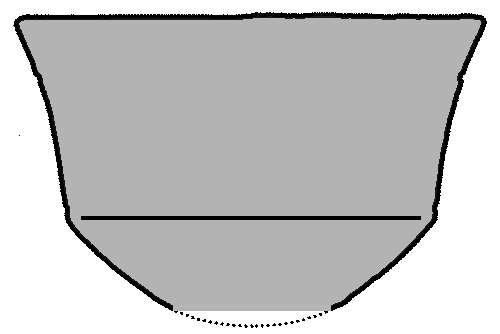
\includegraphics[width=.1\textwidth]{fig/Abb_GefFormen/G2f_MSG87-101-49.png} & 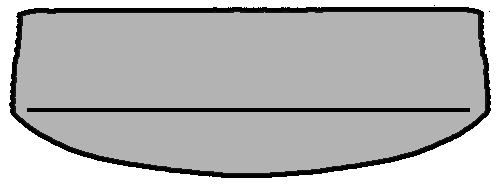
\includegraphics[width=.1\textwidth]{fig/Abb_GefFormen/G2g_GE2_BLK87-1-1-3-1-2.png} & 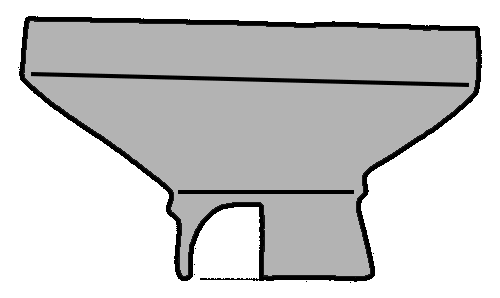
\includegraphics[width=.1\textwidth]{fig/Abb_GefFormen/G2g_MUN87-1-0-2-3-1.png} & 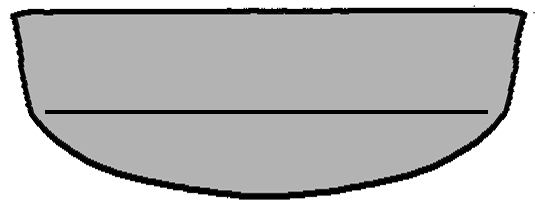
\includegraphics[width=.1\textwidth]{fig/Abb_GefFormen/G8c_Coart1907_TafXII175_neu.png} &  & Schalenförmige Gefäße mit abknickender Wandung & \\[.11\textwidth]
 & \textbf{H} & 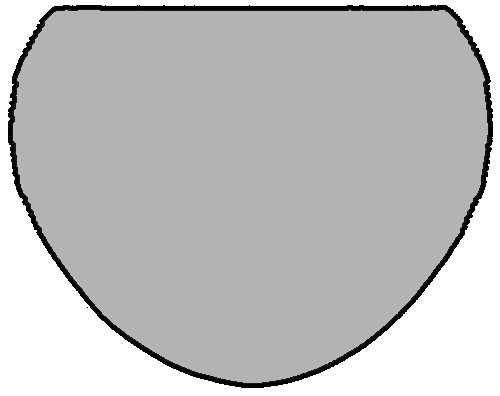
\includegraphics[width=.1\textwidth]{fig/Abb_GefFormen/G8e_kpt85-101-10.png} & 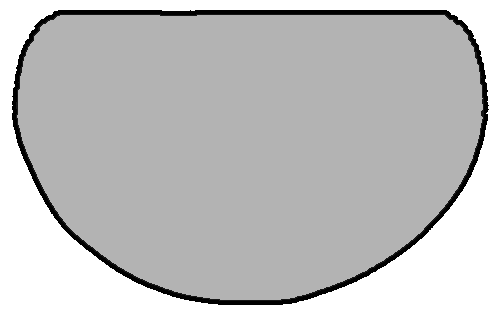
\includegraphics[width=.1\textwidth]{fig/Abb_GefFormen/G8d_MBN85-501-1.png} &  &  &  &  &  & Schalenförmige Gefäße mit konvexer Wandung und einbiegendem Rand & \\[.11\textwidth]
 & \textbf{I} & 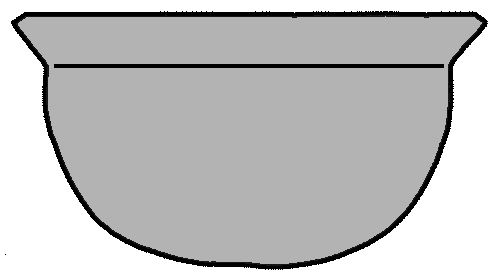
\includegraphics[width=.1\textwidth]{fig/Abb_GefFormen/G8b_BYN87-101-9.png} & 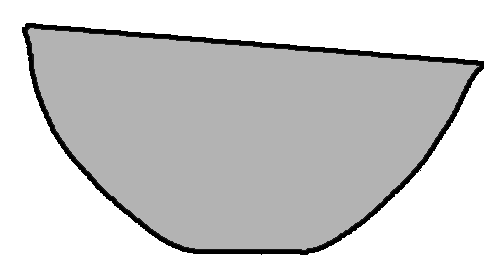
\includegraphics[width=.1\textwidth]{fig/Abb_GefFormen/G9a_DON85-102-120.png} & 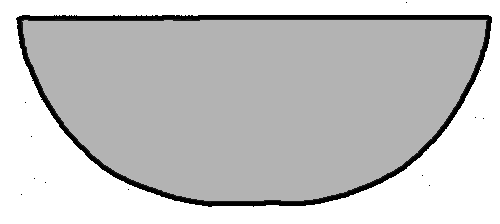
\includegraphics[width=.1\textwidth]{fig/Abb_GefFormen/G8a_BTW87-101-43.png} & 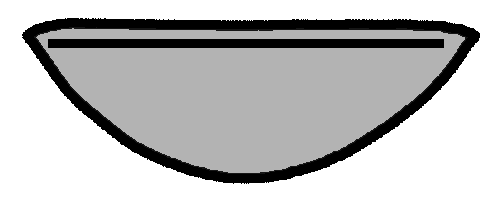
\includegraphics[width=.05\textwidth]{fig/Abb_GefFormen/G8a2_ngk01_PDM87-101-105.png} &  &  &  & Schalenförmige Gefäße mit konvexer Wandung & \\[.11\textwidth]
 & \textbf{J} & 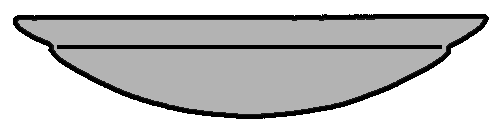
\includegraphics[width=.1\textwidth]{fig/Abb_GefFormen/G12a_NGO87-102-30.png} &  &  &  &  &  &  & Tellerförmige Gefäße & \\[.11\textwidth]
%\bottomrule
\end{sftabular}
}}
	\caption{Keramik: Gefäßtypen (G6 nach \cite[Taf.~XII.175]{Coart.1907}).}
	\label{tab:Keramik_GefFormen}
\end{figure*}

\noindent Von zentraler Bedeutung sind die Eigenschaften der im Scherben enthaltenen nichtplastischen Partikel. Diese wurden entsprechend ihrer Größe und Art sowie dem Anteil, in dem sie vorkommen, aufgenommen. Die Größe der Partikel wurden entsprechend der international anerkannten \textit{Wentworth-Grainsize-Scale} \parencite[381 Tab.~1, 388 Abb.~3]{Wentworth.1922} aufgenommen, wobei fünf Größenklassen unterschieden wurden (Tab.~\ref{tab:Keramik_PartikelGr}).\footnote{Die Bestimmung der Größenklassen erfolgte makroskopisch sowie unter Zuhilfenahme einer 10-fach vergrößernden Lupe in Referenz zu einer Korngrößen-Karte der Firma \textit{Precision Core} (Denver).} Die Verrundung und Sortierung der Partikel wurden nicht systematisch aufgenommen. Der Anteil an nichtplastischen Partikeln im Scherben wurde auf Basis einer Vergleichstafel zum Abschätzen von Anteilsklassen ermittelt \parencites[32]{Kinne.2009}[nach][]{Hodgson.1976}. Die Ansprache der Art der Partikel erfolgte basierend auf makroskopisch sichtbaren Kriterien und den Erfahrungen des Autors.

Zusätzlich zu diesen Eigenschaften der im Scherben beobachtbaren nichtplastischen Partikel erfolgte eine systematische Aufnahme der farblichen Zonierung der Stücke. Die farblichen Abstufungen der Keramik wurden mittels einer fünf Zonen umfassenden Unterteilung der Stücke sowie sechs Farbklassen\footnote{Zur Frage der Nutzung von Farbklassen entgegen der Aufnahme individueller MUNSELL-Farbwerte sei an dieser Stelle exemplarisch auf die Diskussion durch \textcite[38]{Keding.1997} verwiesen.} umfassenden Systematik erfasst (Tab.~\ref{tab:Keramik_Farbe}). Die fünf unterschiedenen Zonen gliedern sich in die äußere und innere Oberfläche des Stücks sowie drei Zonen im Profil beziehungsweise Bruch: den Bereich nahe der Außen- sowie Innenseite sowie der Kernbereich selbst. Die Oberflächenfarbe wurde als \textit{basic surface colour} nach \textcite[44\,f.]{Nordstrom.1972} aufgenommen. Die Ausbildung der Grenze zwischen den farblichen Zonen im Profil wurde in Anlehnung an \textcite[27]{Kinne.2009} umschreibend erfasst.

\begin{figure*}[p]
	\noindent\begin{minipage}[b]{\columnwidth}
		\centering
		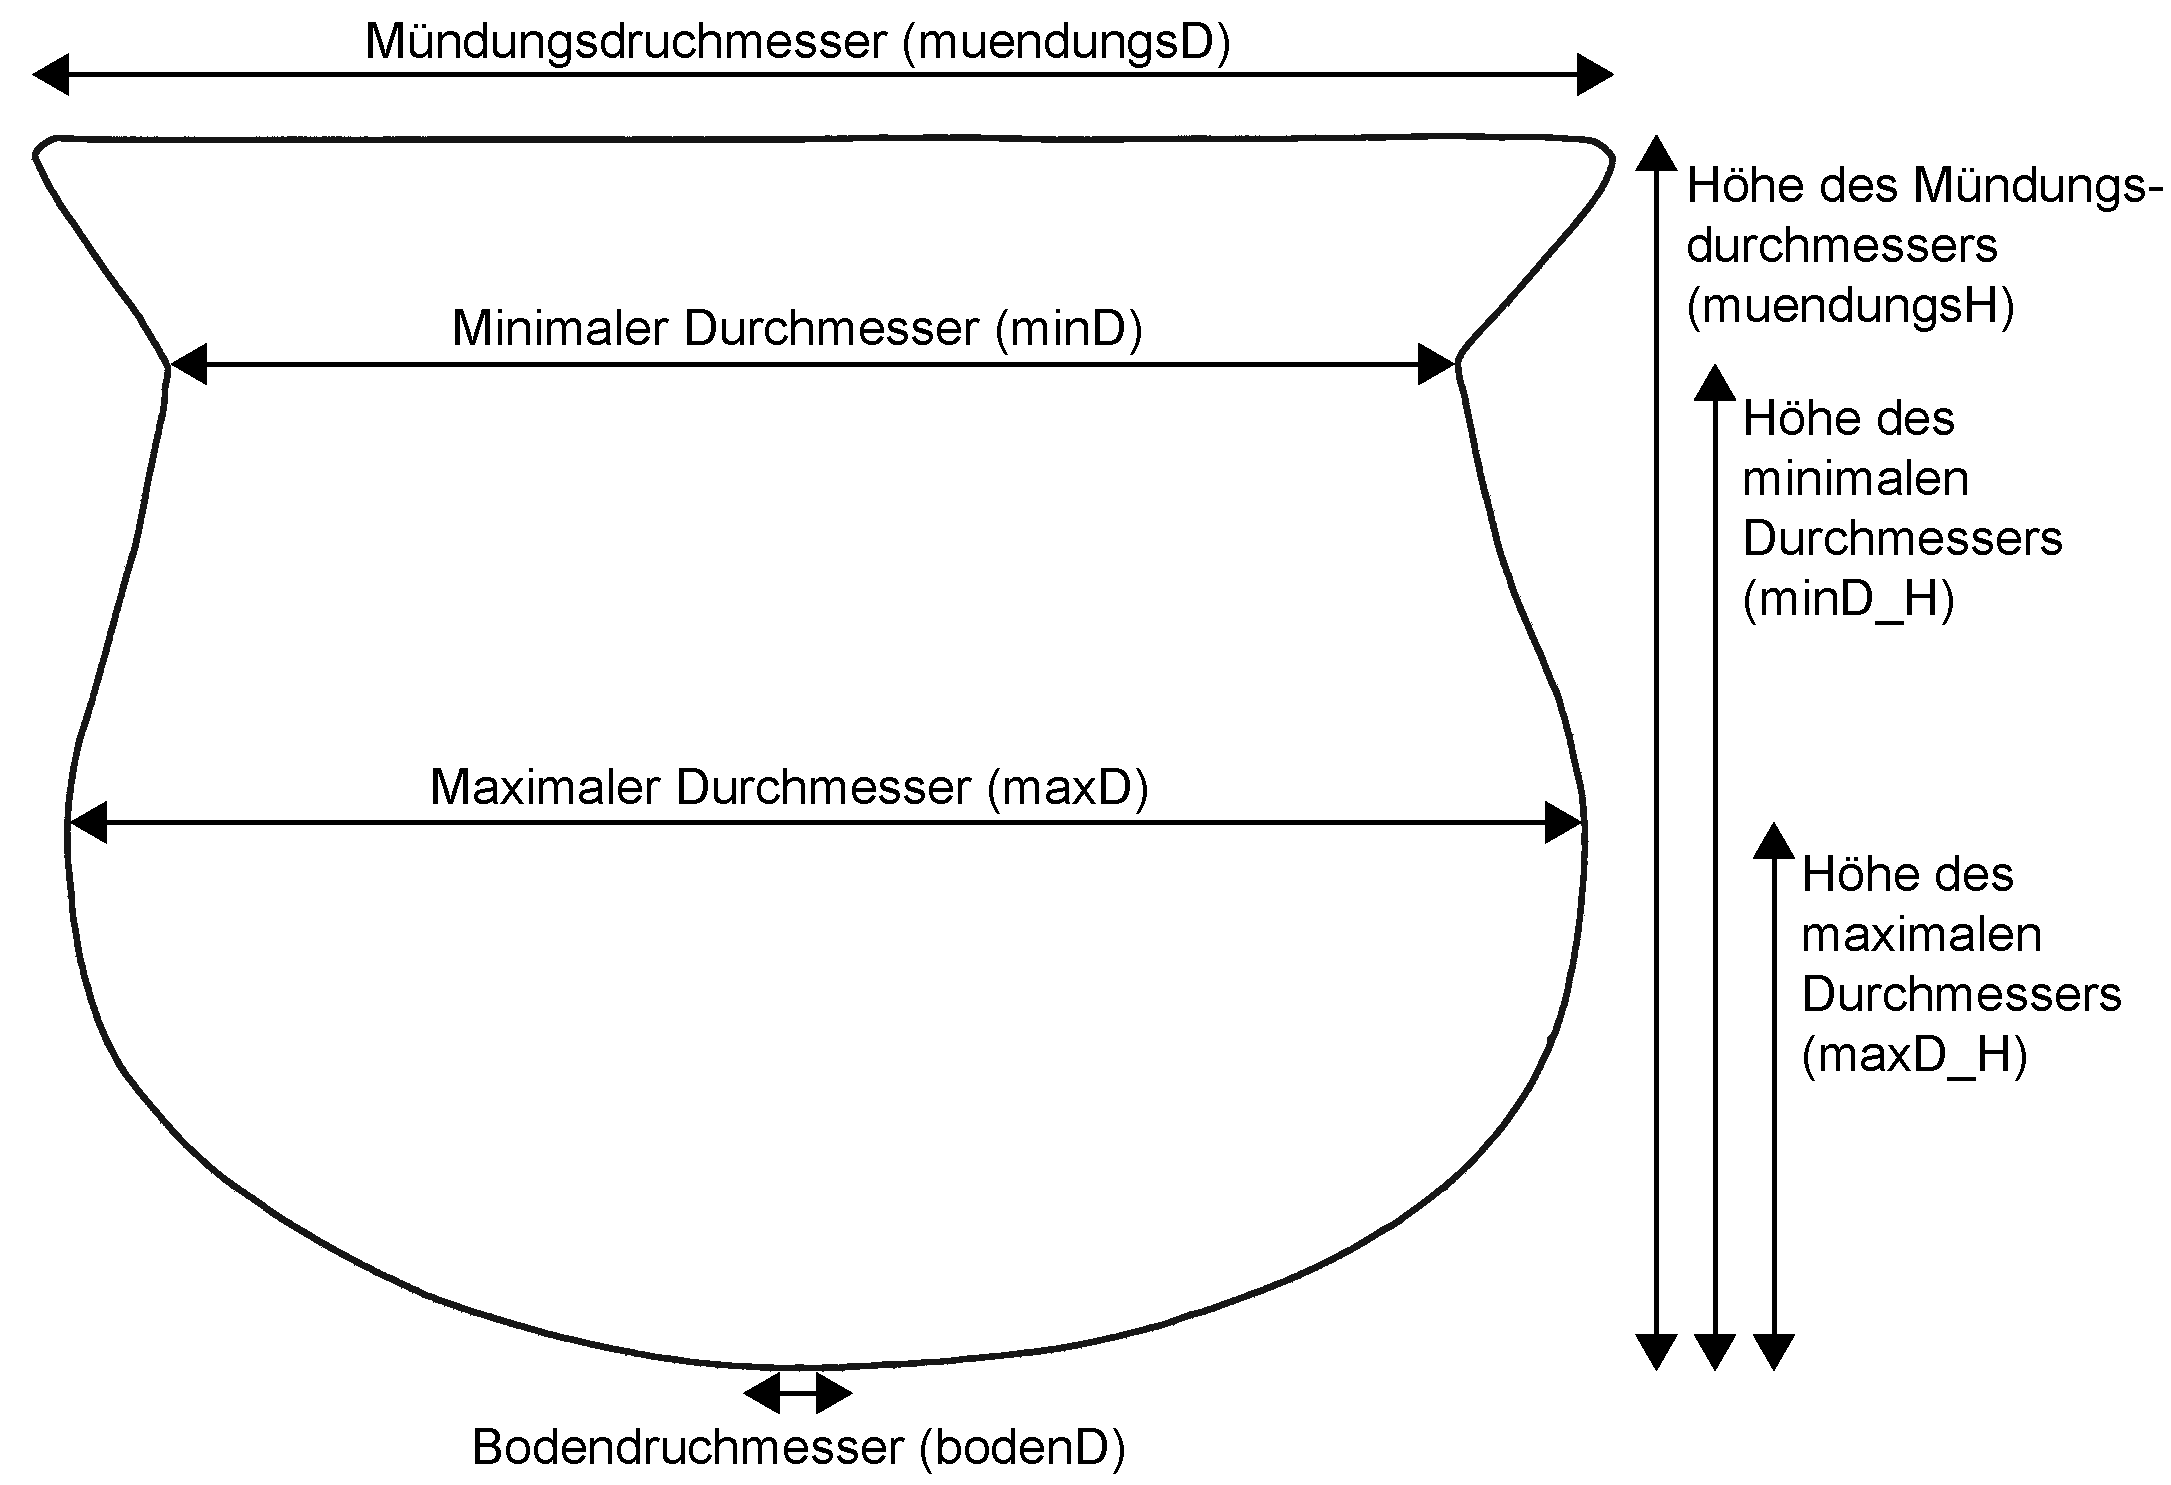
\includegraphics[width=\textwidth]{fig/GefaesseAbmessungenSystematik.pdf}
		\captionof{figure}{Keramik: Aufnahmeschema für die Gefäßabmessungen \parencite[nach][]{Wicke.2011}.\label{fig:GefAbmessungen_Schema}\\}
		\vspace{4cm}\captionof{figure}{Keramik: Systematik der Gefäßzonen, die für die Beschreibung morphologischer Ausprägungen sowie Verzierungen herangezogen wurde.\label{fig:Keramik_VerzZonen}}
	\end{minipage}\hfill
	\noindent\begin{minipage}[b]{\columnwidth}
		\centering
		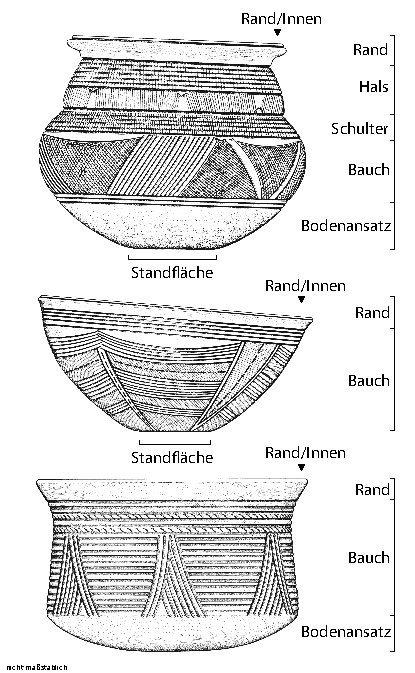
\includegraphics[width=\textwidth]{fig/Keramik_Systematik_Verzierungszonen.pdf}
	\end{minipage}
\end{figure*}

Die Oberflächenstruktur der Stücke wurde unter Referenz auf eine grobe, subjektive Ansprache als \textit{glatt}, \textit{leicht rau} oder \textit{rau} erfasst. Die bei der Keramik der Mandombe-Gruppe (Kap.~\ref{sec:MDB-Gr}) beobachtete Schlicker-Rauung der Gefäßunterteile (siehe Taf.~47.24) wurde als entsprechende Eigenschaft der Oberfläche erfasst. Spezifische Behandlungen der Oberfläche, wie Engoben, wurden hingegen gesondert, gemeinsam mit Anhaftungen an den Stücken aufgenommen. Für diese Oberflächenbehandlungen wurde keine Systematik herangezogen, die Beobachtungen wurden beschreibend in der Datenbank verzeichnet.

Die sich aus diesen technischen Eigenschaften des Scherbens ergebenden Gruppen wurden als \textit{Fabrics} konzeptualisiert und werden in Kap.~\ref{sec:Herstellung2_Fabric} detailliert besprochen.

%\pagebreak
\subsubsection{Form}

\paragraph{Gefäßform}\hspace{-.5em}|\hspace{.5em}%
Im Rahmen der Auswertung der Gefäßkeramik konnten zehn verschiedene Grundformen unterschieden werden (Abb.~\ref{tab:Keramik_GefFormen} A--J). Diese ließen sich weiter in Varianten (Abb.~\ref{tab:Keramik_GefFormen} 1--7) differenzieren, wodurch sich 41 Gefäßtypen ableiten ließen. Die gewählte Systematisierung der beobachteten Formen war für die angestrebte diachrone Untersuchung unerlässlich, da sich Gefäßformen einerseits zwar im Zeit-Raum-Kontinuum verändern, andererseits sich die Grundformen aber auch immer wiederholen \parencite[86]{Saev.2015}. Die von \textcite[39\, f.]{Wotzka.1995} genutzte Systematisierung, die nur grobe Grundformen wie Topf, Schale, Teller oder Flasche kennt und zusammengenommen 115 Gefäßtypen umfasst, konnte aufgrund ihrer spezifisch auf das Material aus dem Inneren Kongobecken zugeschnittenen Ausprägung nicht übernommen werden.\columnbreak

Insgesamt war bei 2178 Gefäßeinheiten (41\,\%) eine Ansprache der Gefäßform möglich. Die Proportionen der GE wurden, wo das Abnehmen der entsprechenden Maße möglich war, unter Einsatz von sieben Messstrecken systematisch erfasst \parencite[Abb.~\ref{fig:GefAbmessungen_Schema}; siehe][]{Wicke.2011}.\footnote{Im Laufe der Materialaufnahme erwies es sich als problematisch, dass das verwendete Aufnahmeschema für die Höhenwerte von der Standfläche eines Gefäßes ausgeht. Bei einer hohen Zahl von GE fehlte der untere Gefäßteil. Die Höhen der Randabschlüsse und minimaler sowie maximaler Durchmesser ließen sich so nicht aufnehmen. Da das Problem erst spät in der Aufnahme zu Tage trat, wurde von einer systematischen Anpassung der Vermessung abgesehen. In Fällen, in denen eine Bestimmung der fehlenden Partie in akzeptabler Weise möglich schien, wurde die hypothetische Position der Standfläche rekonstruiert und protokolliert.} Die Abmessungen wurden mit einer Messgenauigkeit von 0,5\,cm aufgenommen, wodurch die Proportionen der von Hand aufgebauten Keramik des Arbeitsgebiets angemessen repräsentiert sind.\footnote{Der Unterschied zwischen Mündungsweite, der tatsächlichen Gefäßöffnung und dem Randdurchmesser wurde nicht ausdifferenziert \parencite[siehe][88]{Saev.2015}.}

Die morphologischen Ausprägungen einzelner GE, wie auch die Verzierung (siehe Kap.~\ref{sec:AufnahmeVerzierungen}), wurden mit Bezug auf vordefinierte Gefäßzonen aufgenommen (Abb.~\ref{fig:Keramik_VerzZonen}). Die Abgrenzung der einzelnen Zonen wurde auf Basis markanter Wendepunkte am Profilverlauf der GE vorgenommen.

\begin{figure*}[p]
	\noindent\begin{minipage}[b]{\columnwidth}
		\centering
		{\footnotesize
			\begin{sftabular}{@{} >{\centering\arraybackslash} m{.01\textwidth} >{\centering\arraybackslash} m{.19\textwidth} >{\centering\arraybackslash} m{.19\textwidth} >{\centering\arraybackslash} m{.19\textwidth} >{\centering\arraybackslash} m{.19\textwidth}@{}}
				%\toprule
				& \textbf{1} & \textbf{2} & \textbf{3} & \textbf{4} \\
				%\midrule
				\textbf{A} & 
\includegraphics[height=.2\textwidth]{fig/Abb_RandFormen/A1.pdf} & 
\includegraphics[height=.2\textwidth]{fig/Abb_RandFormen/A2.pdf} & \includegraphics[height=.2\textwidth]{fig/Abb_RandFormen/A3.pdf} & \includegraphics[height=.2\textwidth]{fig/Abb_RandFormen/A4.pdf} \\
				\textbf{B} & \includegraphics[height=.2\textwidth]{fig/Abb_RandFormen/B1.pdf} & \includegraphics[height=.2\textwidth]{fig/Abb_RandFormen/B2.pdf} & \includegraphics[height=.2\textwidth]{fig/Abb_RandFormen/B3.pdf} & \\
				\textbf{C} & \includegraphics[height=.2\textwidth]{fig/Abb_RandFormen/C1.pdf} & \includegraphics[height=.2\textwidth]{fig/Abb_RandFormen/C2.pdf} & \includegraphics[height=.2\textwidth]{fig/Abb_RandFormen/C3.pdf} & \\
				%\bottomrule
		\end{sftabular}}\vspace{2em}
		\captionof{figure}{Keramik: Unterschiedene Randformen. Grundformen A--B als Zeilen und Varianten in Spalten.\label{tab:Keramik_RandFormen}}
	\end{minipage}\hfill
	\noindent\begin{minipage}[b]{\columnwidth}
		\centering
		{\footnotesize
			\begin{sftabular}{@{}m{.1\textwidth}m{.1\textwidth}m{.69\textwidth}@{}}
				\toprule
				& \textbf{Typ} & \textbf{Beschreibung} \\
				\midrule
				\includegraphics[height=.1\textwidth]{tbl/Tab_MdgFormen/M1_ATANGANA1988OkoloS162_1.png} & M1 & rund \\
				\includegraphics[height=.1\textwidth]{tbl/Tab_MdgFormen/M2_ATANGANA1988OkoloS162_2.png} & M2 & spitz \\
				\includegraphics[height=.1\textwidth]{tbl/Tab_MdgFormen/M3_ATANGANA1988OkoloS162_3.png} & M3 & gerade/flach/horizontal abgestrichen \\
				\includegraphics[height=.1\textwidth]{tbl/Tab_MdgFormen/M4_ATANGANA1988OkoloS162_4.png} & M4 & gerillt \\
				\includegraphics[height=.1\textwidth]{tbl/Tab_MdgFormen/M5_schraegAussen.png} & M5 & schräg nach außen abgestrichen \\
				\includegraphics[height=.1\textwidth]{tbl/Tab_MdgFormen/M6_schraegInnen.png} & M6 & schräg nach innen abgestrichen \\
				\bottomrule
		\end{sftabular} }
		\captionof{table}{Keramik: Übersicht der Randlippe \parencite[erweitert nach][162\,f. Tab.~24]{Atangana.1988}.\label{tab:MdgFormen}}
	\end{minipage}
\end{figure*}

\begin{figure*}[!tb]
	\centering
	\includegraphics[width=.95\textwidth]{fig/Wotzka1995_440Taf6_modDS.jpg}
	\caption{Keramik: Bodenformen \parencite[nach][440 Taf.~6]{Wotzka.1995}.}
	\label{fig:Keramik_BodenFormen}
\end{figure*}

\paragraph{Randform}\hspace{-.5em}|\hspace{.5em}\label{sec:Randform}
Die Aufnahme der Ränder erfolgte gemäß einer Systematik, die sich in erster Linie an der grundsätzlichen Ausrichtung des Randes orientiert. Differenziert wurden parallele, ausbiegende sowie einbiegende Ränder (Abb.~\ref{tab:Keramik_RandFormen}: A--C). Innerhalb dieser Grundtypen wurden mehrere charakteristische Varianten unterschieden. Parallele Ränder können neben der einfachen Grundform auch als umgelenkte, T-förmige sowie verdickte Formen vorkommen (Abb.~\ref{tab:Keramik_RandFormen}: A2--A4). Aus- wie einbiegende Ränder wurden noch in konkave sowie konvexe Varianten unterschieden (Abb.~\ref{tab:Keramik_RandFormen}: B2--B3, C2--C3):

\vspace{1em}
\noindent\begin{tabular}{@{}ll@{}}
A1 & parallel \\
A2 & umgelegt \\
A3 & T-förmig \\
A4 & verdickt \\
B1 & ausbiegend \\
B2 & konkav ausbiegend \\
B3 & konvex ausbiegend \\
C1 & einbiegend \\
C2 & konkav einbiegend \\
C3 & konvex einbiegend \\
\end{tabular}
\vspace{1em}

\noindent An die Grundform angefügte Parameter \enquote{.1} sowie \enquote{.2} zeigen \textit{kurze} beziehungsweise \textit{lange} Varianten der entsprechenden Randform an. Spezifischere und diagnostische Variationen der Grundformen wurden im weiteren Verlauf der Aufnahme durch Hinzusetzen individueller Zählnummern, beginnend ab dem Schlüssel-Zusatz \enquote{.3}, angefügt. Insgesamt ergaben sich zehn Grundformen der Randgestaltung (Abb.~\ref{tab:Keramik_RandFormen}) sowie 26 unterscheidbare Variationen.\footnote{Wie bereits bei den Gefäßformen (Abb.~\ref{tab:Keramik_GefFormen}) spiegelt die gewählte Form der Systematisierung das Bestreben wider, die Aufnahme des Untersuchungsmaterials vor dem Hintergrund der dieser Arbeit zugrundeliegenden diachronen Fragestellungen durchzuführen.}

Die häufigste Randform, die einfach ausbiegenden Ränder (B1), macht 24,8\,\% aller bestimmten Randformen aus, gefolgt von konkav ausbiegenden Rändern (B2), die in 13,3\,\% aller Fälle beobachtet wurden. Die kurze Variante gerade ausbiegender Ränder (B1.1) macht 11,7\,\% aus, während parallel, gerade aufsteigende Ränder (A1) auf einen Anteil von 10\,\% kommen. Alle übrigen Varianten liegen jeweils im Bereich von unter 7\,\%. Zusammengenommen repräsentieren diese, einzeln nur selten vertretenen Formen, 40\,\% der aufgenommen Gefäßränder. Werden die unterschiedenen Variationen den jeweiligen Grundformen (Abb.~\ref{tab:Keramik_RandFormen}) zugerechnet, sind insgesamt 68,5\,\% aller Rändern ausbiegend (B), während 25\,\% parallel (A) verlaufen und nur 6,5\,\% einbiegend (C) sind.

\paragraph{Randlippe}\hspace{-.5em}|\hspace{.5em}%
Die Ausprägung der Randlippe, in diesem Zusammenhang auch \textit{Gefäßmündung} genannt, wurde in Anlehnung an die von \textcite[162f Tab.~24]{Atangana.1988} genutzte Systematik losgelöst von der Randform aufgenommen (Tab.~\ref{tab:MdgFormen}).\footnote{\textcite[48]{Wotzka.1995} erfasste die Ausprägung der Randlippe nicht separat, sie bildete vielmehr eine mögliche Variation des \textit{Randtyps} ab. Ähnlich ging auch \textcite[110]{Jesse.2003} vor.} Die Einteilung Atanganas wurde dabei um die beiden Formen M5 sowie M6, die schräg nach außen oder innen abgestrichene Randlippen widerspiegeln, erweitert. Die Varianten M1 bis M5 sind jeweils in Häufigkeiten zwischen 13,5 bis 26,4\,\% vertreten, schräg nach innen abgestrichene Randlippen des Typs M6 kommen mit nur 3,9\,\% deutlich seltener vor.

\paragraph{Bodenform}\hspace{-.5em}|\hspace{.5em}\label{sec:Bodenform}
Die Unterscheidung der Ausformung des Bodens gründete sich auf die von \textcite[440 Taf.~6]{Wotzka.1995} aufgestellten Systematik, die um eine Form B15 erweitert wurde. Die neue Bodenform B15 beschreibt Gefäße, die auf einzelnen \textit{Füßchen} stehen. Im untersuchten Material fanden sich lediglich zwei GE mit drei symmetrisch am Unterteil eines ansonsten rund ausgeformten Bodens angebrachten \textit{Füßchen} (Taf.~1.2, 2.1). Im Detail wurden folgende Bodenformen unterschieden (Abb.~\ref{fig:Keramik_BodenFormen}):
\setlength\LTleft{0pt}
\vspace{.25em}
\noindent\begin{tabular}{@{}ll@{}}
	B1 & Rundboden \\
	B2 & Linsenboden \\
	B3 & Spitzboden \\
	B4 & einfacher Flachboden \\
	B5 & innen aufgewölbter Flachboden  \\
	B6 & Flachboden mit konkaver Standfläche \\
	B7 & Omphalosboden \\
	B8 & Riefenprofilierter Flachboden \\
	B9 & Profiliert abgesetzter Flachboden \\
	B10 & Riefenabgesetzter Flachboden \\
	B11 & abgesetzter Flachboden \\
	B12 & Flachboden mit einziehender Unterseite\\
\end{tabular}
%\vspace{1em}

%\setlength\LTleft{0pt}
\vspace{.25em}
\noindent\begin{tabular}{@{}ll@{}}
	B13 & Standring / Hohlfuß \\
	B14 & massiver Standfussboden \\
	B15 & Boden mit abgesetzten Standfüßen \\
\end{tabular}
\vspace{1em}

\noindent Insgesamt konnte die Bodenform lediglich bei 6\,\% aller GE angesprochen werden. Dieser geringe Anteil liegt zu einen gewissen Grad an den Schwierigkeiten, die mit der Ansprache runder Böden (B1) verbunden sind, die leicht als Fragmente der Gefäßwandung fehlinterpretiert werden können. Zusammengenommen machen runde Böden (B1) knapp 49\,\% aller bestimmter Böden aus. Einfache Flachböden (B4) kommen mit 24\,\% am zweithäufigsten vor. Gefolgt werden sie von Linsenböden (B2) mit 6\,\%, Standringböden mit Hohlfuß (B13) mit ebenfalls 6\,\% sowie 5\,\% Flachböden mit konkaver Standfläche (B6). Die übrigen Formen kommen lediglich als Einzelfunde beziehungsweise bei weniger als zehn GE vor. Der von \textsc{Wotzka} (ebd. 440 Taf.~6) beschriebe Typ B14 wurde nicht beobachtet.

\subsubsection{Verzierung}\label{sec:AufnahmeVerzierungen}

Die Verzierungen der Keramik wurden für jede Gefäßeinheit individuell und in Referenz zur Gefäßregion aufgenommen (siehe Abb.~\ref{fig:Keramik_VerzZonen}).\footnote{Während formale Ansprachen wie die Gefäßform in einer 1:n-Beziehung in einer Datenbank abgebildet werden können (eine GE kann lediglich eine Gefäßform oder Randform aufweisen), können verschiedene Verzierungen auf verschiedenen Gefäßbereichen unterschiedlich häufig vorkommen. Die vorliegende Kardinalität der Entitätstypen \textit{Objekt}, \textit{Gefäßposition} und \textit{Verzierungselement} können in dem genutzten relativen Datenbankschema nicht direkt abgebildet werden. Die Entitäten jeder dieser Entitätstypen können mit beliebig vielen Entitäten der anderen beiden Entitätstypen in Beziehung stehen. Konkret ist hiermit gemeint, dass eine GE an verschiedenen Stellen auch mehrere Verzierungselemente aufweisen kann. Als Lösung wird eine Konkordanztabelle genutzt, welche die Primärschlüssel der genannten Entitätstypen als Fremdschlüssel-Paare beinhaltet. Die Beziehungen der drei Entitätstypen werden im Datenmodell durch drei getrennte 1:n-Beziehungen aufgelöst.} Basierend auf der Kombination aus Verzierungstechnik und -motiv wurden Verzierungselemente erarbeitet (Tab.~\ref{tab:Verzierungselemente}; Abb.~\ref{fig:Keramik_VerzSystematik}).\footnote{Die Klassifizierung der einzelnen Verzierungselemente lehnt sich dabei stark an \textsc{Wotzka} (1995) an, nimmt aber auch Aspekte aus Systematiken für die Bandkeramik \parencites{Stehli.1973}{Stehli.1977}{Kneipp.1998} und das südfranzösische Frühneolithikum auf \parencites[126\,f. Abb.~3]{Manen.2002}[auch bei][]{Linstadter.2013}. Die grafische Zusammenstellung der Klassifizierung in Abb.~\ref{fig:Keramik_VerzSystematik} folgt der Darstellungsweise von \textcite[80\,f. Abb.~39]{Keding.1997}.} Diese bilden in der Aufnahme der Verzierungen wie deren Auswertung die analytische Grundeinheit.

\begin{figure*}[p]
 \centering
 \includegraphics[width=.85\textwidth]{fig/VerzierungenSystematik.pdf}
 \caption{Keramik: Verzierungstechniken, Verzierungswerkzeuge und Verzierungselemente.}
 \label{fig:Keramik_VerzSystematik}
\end{figure*}

%\end{multicols}
%\afterpage{%
%\clearpage
\begin{table*}[p]

\begin{multicols}{2}
\noindent
{\scriptsize\begin{sftabular}{@{}m{.05\columnwidth} m{.1\textwidth} m{.63\columnwidth}@{}}
\toprule
\multicolumn{2}{@{}l@{}}{\textbf{Schlüssel}} &  \textbf{Kurzbeschreibung} \\
\midrule
01.1 & \includegraphics[width=.1\textwidth]{tbl/Tab_VerzElemente/V03a_PIK87-1-7-1.png} & \textit{Schachbrett}-Muster aus horizontalen und vertikalen Ritzlinien \\
01.2 & \includegraphics[width=.1\textwidth]{tbl/Tab_VerzElemente/V03b_PIK87-1-6-16.png} & \textit{Schachbrett}-Muster aus diagonalen Ritzlinien \\
01.3 & \includegraphics[width=.1\textwidth]{tbl/Tab_VerzElemente/V03c_PIK87-1-8-6.png} & \textit{Schachbrett}-Muster aus horizontalen und diagonalen Ritzlinien \\
01.4 & \includegraphics[width=.1\textwidth]{tbl/Tab_VerzElemente/V03d_PIK87-1-9-7.png} & \textit{Schachbrett}-Muster aus diagonalen und vertikalen Ritzlinien \\
01.5 & \includegraphics[width=.1\textwidth]{tbl/Tab_VerzElemente/V01b_PIK87-1-5-7.png} & Wellenlinien \\
01.6 & \includegraphics[width=.1\textwidth]{tbl/Tab_VerzElemente/V12a1_MSG87-102-8.png} & Zickzack-Linien \\
01.7 & \includegraphics[width=.1\textwidth]{tbl/Tab_VerzElemente/V12c_Gef9_CAM07-3-1-278-306.png} & Rillen in Fischgrät-Muster \\
01.8 & \includegraphics[width=.1\textwidth]{tbl/Tab_VerzElemente/V04d_PIK87-101-43-46.png} \includegraphics[width=.1\textwidth]{tbl/Tab_VerzElemente/V04e_NGO87-102-28-29.png} & Rillen gefüllte Flächen (Dreiecke, Rauten u.~a.) \\
01.9 & \includegraphics[width=.1\textwidth]{tbl/Tab_VerzElemente/V10a_PIK87-101-51.png} & feine vertikale oder horizontale Rillen \\
01.10 & \includegraphics[width=.1\textwidth]{tbl/Tab_VerzElemente/V10b_PIK87-101-40.png} & feine diagonale Rillen \\
01.11 & \includegraphics[width=.1\textwidth]{tbl/Tab_VerzElemente/V11b1_LKW87-186-1-2-5.png} & Muster aus überkreuzten Rillen \\
02.1 & \includegraphics[width=.1\textwidth]{tbl/Tab_VerzElemente/V01a_PIK87-1-8-6.png} & horizontale Riefen \parencite[siehe Muster \enquote{ISpeg5} von][251 Abb. 30.5 ]{GouemGouem.20102011} \\
02.2 & \includegraphics[width=.1\textwidth]{tbl/Tab_VerzElemente/V01c_PIK87-1-8-6.png} & vertikale Riefen \\
\bottomrule
\end{sftabular}}

\noindent
{\scriptsize\begin{sftabular}{@{}m{.05\columnwidth} m{.1\textwidth} m{.63\columnwidth}@{}}
\toprule
\multicolumn{2}{@{}l@{}}{\textbf{Schlüssel}} &  \textbf{Kurzbeschreibung} \\
\midrule
02.3 & \includegraphics[width=.1\textwidth]{tbl/Tab_VerzElemente/V01e_PIK87-1-8-6.png} & diagonale Riefen \\
02.4 & \includegraphics[width=.1\textwidth]{tbl/Tab_VerzElemente/V01e2_MLB85-1-3-2-5-35.png} & horizontales Band aus kurzen diagonalen Riefen \\
02.5 & \includegraphics[width=.1\textwidth]{tbl/Tab_VerzElemente/V01d_PIK87-101-7.png} & gebogene Riefen \\
02.6 & \includegraphics[width=.1\textwidth]{tbl/Tab_VerzElemente/V01f_MUN87-2-1-1-5-2.png} & spitz zusammenlaufende gebogene Riefen \\
02.7 & \includegraphics[width=.1\textwidth]{tbl/Tab_VerzElemente/V04c_PIK87-1-3-9.png} & sehr breite Riefen (\textgreater\,5\,mm) \\
03.1 & \includegraphics[width=.1\textwidth]{tbl/Tab_VerzElemente/V06e.png} & große Eindrücke, Fingereindrücke \\
04.1 & \includegraphics[width=.1\textwidth]{tbl/Tab_VerzElemente/V02a_PIK87-1-8-6.png} & Wiegeband mit Kamm \\
04.2 & \includegraphics[width=.1\textwidth]{tbl/Tab_VerzElemente/V02b_MUN87-2-1-1-4-2.png} & Wiegeband (siehe Muster \enquote{IIIPla1z} von \textsc{Gouem Gouem} 2010/2011: 117 Abb. 9.3.a ) \\
04.3 & \includegraphics[width=.1\textwidth]{tbl/Tab_VerzElemente/V05e_INS87-102-2.png} & gruppierte Eindrücke \\
04.4 & \includegraphics[width=.1\textwidth]{tbl/Tab_VerzElemente/V05f_SSL87-101-143.png} & gegenständige Eindrücke \\
04.5 & \includegraphics[width=.1\textwidth]{tbl/Tab_VerzElemente/V05j_SSL87-101-5.png} & kleine Flächen aus gegenständigen, halbrunden Eindrücken \\
04.6 & \includegraphics[width=.1\textwidth]{tbl/Tab_VerzElemente/V05h_DON85-102-a.png} & flache, winkelige Eindrücke \\
04.7 & \includegraphics[width=.1\textwidth]{tbl/Tab_VerzElemente/V05i1_MLB85-1-2-3.png} & kleine Kreisaugen-Eindrücke \\
& & \\[1mm]
\bottomrule
\end{sftabular}}
\end{multicols}
\caption{Keramik: Verzierungselemente. Für die ersten beiden Stellen der Schlüsselzahl -- die  Verzierungstechnik -- siehe \textsc{Wotzka} (1995: 44 Tab.~3).}
\label{tab:Verzierungselemente}
\end{table*}

\addtocounter{table}{-1}
\begin{table*}[p]
\begin{multicols}{2}
\noindent
{\scriptsize\begin{sftabular}{@{}m{.05\columnwidth} m{.1\textwidth} m{.63\columnwidth}@{}}
\toprule
\multicolumn{2}{@{}l@{}}{\textbf{Schlüssel}} &  \textbf{Kurzbeschreibung} \\
\midrule
04.8 & \includegraphics[width=.1\textwidth]{tbl/Tab_VerzElemente/V09l_MKA87-102-1.png} & dreieckige Eindrücke/Dreieckstempel \\
04.9 & \includegraphics[width=.1\textwidth]{tbl/Tab_VerzElemente/V09j_MIS87-101-56.png} & flächig angeordnete, horizontale Bänder kleiner Eindrücke \\
04.10 & \includegraphics[width=.1\textwidth]{tbl/Tab_VerzElemente/V09k_MIS87-101-56.png} & lose flächig verteilte kleine Eindrücke \\
04.11 & \includegraphics[width=.1\textwidth]{tbl/Tab_VerzElemente/V09i2_MKL85-101-114.png} & runde bis leicht ovale Eindrücke \\
04.12 & \includegraphics[width=.1\textwidth]{tbl/Tab_VerzElemente/V09a1_PIK87-1-14-1.png} & diagonale Eindrücke \\
04.13 & \includegraphics[width=.1\textwidth]{tbl/Tab_VerzElemente/V09n_SSL87-101-19.png} & leicht gewellte Bänder aus diagonalen oder vertikalen Eindrücken \\
04.14 & \includegraphics[width=.1\textwidth]{tbl/Tab_VerzElemente/V09a2_DON85-102-120.png} & horizontales oder vertikales Band aus linearen Eindrücken \\
04.15 & \includegraphics[width=.1\textwidth]{tbl/Tab_VerzElemente/V09b_PIK87-1-8-10.png} & vertikale Eindrücke \\
04.16 & \includegraphics[width=.1\textwidth]{tbl/Tab_VerzElemente/V09c1_PIK87-1-13-1.png} \includegraphics[width=.1\textwidth]{tbl/Tab_VerzElemente/V09c2_DON85-102-117.png} & Eindrücke in Rillen (siehe Muster \enquote{ISpeg5/ISpeg11} bei \textsc{Gouem Gouem} 2010/2011251, 251 Abb. 30.5) \\
04.17 & \includegraphics[width=.1\textwidth]{tbl/Tab_VerzElemente/V12b_INS87-102-2.png} & gegenständige Dreiecke in horizontalem Band \\
04.18 & \includegraphics[width=.1\textwidth]{tbl/Tab_VerzElemente/V11b2_DON85-102-126.png} & Bänder aus x-förmigen Eindrücken \\
04.19 & \includegraphics[width=.1\textwidth]{tbl/Tab_VerzElemente/V09h1_PDM87-101-12.png} & lange gebogene Eindrücke in Reihen \\
04.20 & \includegraphics[width=.1\textwidth]{tbl/Tab_VerzElemente/V09h2_MIT87-102-19.png} & kurze gebogene Eindrücke (Fingernagel) \\
04.21 & \includegraphics[width=.1\textwidth]{tbl/Tab_VerzElemente/V05i3_MBA11-1-1_DSC_0507_b.png} & Eindrücke mit Kaurischnecken oder Imitation \\
& & \\
\bottomrule
\end{sftabular}}

\noindent
{\scriptsize\begin{sftabular}{@{}m{.05\columnwidth} m{.1\textwidth} m{.63\columnwidth}@{}}
\toprule
\multicolumn{2}{@{}l@{}}{\textbf{Schlüssel}} &  \textbf{Kurzbeschreibung} \\
\midrule
05.1 & \includegraphics[width=.1\textwidth]{tbl/Tab_VerzElemente/V02c_PDM87-101-125.png} & diagonaler Kammeindruck \\
05.2 & \includegraphics[width=.1\textwidth]{tbl/Tab_VerzElemente/V12a3_MKL85-101-105.png} & Band aus zickzackartig angeordneten Kammeindrücken \\
05.3 & \includegraphics[width=.1\textwidth]{tbl/Tab_VerzElemente/V05a_PIK87-1-2-5.png} & Kammeindruck-Bänder \\
05.4 & \includegraphics[width=.1\textwidth]{tbl/Tab_VerzElemente/V05b_PIK87-101-8.png} & flächiger Kammeindruck \\
08 & \includegraphics[width=.1\textwidth]{tbl/Tab_VerzElemente/V07_MUN87-1-0-2-3-6.png} & \textit{Bnfwa-nfwa} \parencite[Muster: siehe][109--111]{Wotzka.1995} \\
09.1 & \includegraphics[width=.1\textwidth]{tbl/Tab_VerzElemente/V06a1_PIK87-1-2-5.png} & Knubben \\
09.2 & \includegraphics[width=.1\textwidth]{tbl/Tab_VerzElemente/V06b_PIK87-101-8.png} & Plastische Leiste \\
12 & \includegraphics[width=.1\textwidth]{tbl/Tab_VerzElemente/V14_Wotzka1995_Taf91-4.png} & Mattenabdruck \\
13.1 & \includegraphics[width=.1\textwidth]{tbl/Tab_VerzElemente/V13_Gef3_CAM07-12-II-2.png} & Durchlochung der Gefäßwandung \\
14.1 & \includegraphics[width=.1\textwidth]{tbl/Tab_VerzElemente/VB1_YUM87-103-2.png} & Schwarze bis dunkelgraue Bemalung. Die Bemalung erfolgt ausschließlich in Streifen. Eine flächige Bemalung größerer Abschnitte eines Gefäßes wurde nicht beobachtet. \\
14.2 & \includegraphics[width=.1\textwidth]{tbl/Tab_VerzElemente/Vb2_BBS87-Herdgef_E87-04-4.png} & Rote Bemalung. Die Bemalung erfolgt ausschließlich in Streifen sowie in Riefen. Eine flächige Bemalung größerer Abschnitte eines Gefäßes wurde nicht beobachtet. \\
15.1 & \includegraphics[width=.1\textwidth]{tbl/Tab_VerzElemente/V04a_PIK87-1-3-5.png} & diagonaler Kammstrich \\
15.2 & \includegraphics[width=.1\textwidth]{tbl/Tab_VerzElemente/V04b_PIK87-1-2-225.png} & überkreuzter Kammstrich \\
& & \\[1.5mm]
\bottomrule
\end{sftabular}}
\end{multicols}
\caption{Keramik: Verzierungselemente. Für die ersten beiden Stellen der Schlüsselzahl -- die  Verzierungstechnik -- siehe \textsc{Wotzka} (1995: 44 Tab.~3).}
%\label{tab:Verzierungselemente}
\end{table*}

\addtocounter{table}{-1}
\begin{table*}[!tb]
\begin{multicols}{2}
\noindent
{\scriptsize\begin{sftabular}{@{}m{.05\columnwidth} m{.1\textwidth} m{.63\columnwidth}@{}}
\toprule
\multicolumn{2}{@{}l@{}}{\textbf{Schlüssel}} &  \textbf{Kurzbeschreibung} \\
\midrule
15.3 & \includegraphics[width=.1\textwidth]{tbl/Tab_VerzElemente/V05i2a_PIK87-101-17.png} \includegraphics[width=.1\textwidth]{tbl/Tab_VerzElemente/V05i2b_MTB85-101-12.png} & in Kammstrich-Technik hergestellte konzentrische, teilweise sich überlagernde Kreis-Muster \\
17.1 & \includegraphics[width=.1\textwidth]{tbl/Tab_VerzElemente/V06a2_MLB85-101-18.png} & Ösen \\
17.2 & \includegraphics[width=.1\textwidth]{tbl/Tab_VerzElemente/V06a3_LIB85-101-50.png} & Henkel \\
20.1 & \includegraphics[width=.1\textwidth]{tbl/Tab_VerzElemente/V08m_NGA87-101-22.png} & unklar, möglicherweise Mattenabdruck \\
20.2 & \includegraphics[width=.1\textwidth]{tbl/Tab_VerzElemente/V08n_MBK85-101-11.png} & unklar, möglicherweise Textilabdruck \\
21.1 & \includegraphics[width=.1\textwidth]{tbl/Tab_VerzElemente/V08a_BBL85-101-61.png} & \textit{knotted strip} \parencite[Muster: siehe][191 Abb.~1,C]{LivingstoneSmith.2007} \\
21.2 & \includegraphics[width=.1\textwidth]{tbl/Tab_VerzElemente/V08a1_LivingstoneSmith2007_Fig1A.png} & \textit{twisted string} (Muster: siehe \textsc{Livingstone Smith} 2007: 191 Abb.~1,A) \\
21.3 &  \includegraphics[width=.1\textwidth]{tbl/Tab_VerzElemente/V08a2_LivingstoneSmith2007_Fig1B.png} & \textit{alternate knotted strip} (Muster: ebd. 191 Abb.~1,B) \\
21.4 & \includegraphics[width=.1\textwidth]{tbl/Tab_VerzElemente/V08a3_Mayoretal2005.png} & \textit{Accordion-plaited strip} \parencite[Muster: siehe][36 Abb.~4]{Mayor.2005} \\
21.5 & \includegraphics[width=.1\textwidth]{tbl/Tab_VerzElemente/V08b_KPT85-101-10.png}  & Schnitzroulette, das ein Muster aus gegenläufigen gezähnten Bändern erzeugt \\
& & \\[5mm]
\bottomrule
\end{sftabular}}

\noindent
{\scriptsize\begin{sftabular}{@{}m{.05\columnwidth} m{.1\textwidth} m{.63\columnwidth}@{}}
\toprule
\multicolumn{2}{@{}l@{}}{\textbf{Schlüssel}} &  \textbf{Kurzbeschreibung} \\
\midrule
21.6 & \includegraphics[width=.1\textwidth]{tbl/Tab_VerzElemente/V08c_MTB85-101-94.png} & Schnitzroulette, das ein Muster aus gegenläufigen gezackten Bändern erzeugt \\
21.7 & \includegraphics[width=.1\textwidth]{tbl/Tab_VerzElemente/V08e_ILW85-101-11.png} & Schnitzroulette, das ein rautenförmiges Muster erzeugt, wobei das Zentrum erhaben ist \\
21.8 & \includegraphics[width=.1\textwidth]{tbl/Tab_VerzElemente/V08f_GBA85-101-6.png} & Schnitzroulette wie 21.7 jedoch mit einem erhabenen Zentrum und Grat \\
21.9 & \includegraphics[width=.1\textwidth]{tbl/Tab_VerzElemente/V08g_LIB85-101-28.png} & Schnitzroulette, das ein Muster aus dreieckigen Bändern erzeugt \\
21.10 & \includegraphics[width=.1\textwidth]{tbl/Tab_VerzElemente/V08h_BAT85-101-40.png} & Schnitzroulette wie 21.7 jedoch mit einem eingedrückten Zentrum \\
21.11 & \includegraphics[width=.1\textwidth]{tbl/Tab_VerzElemente/V08i_MBK85-101-15.png} & Schnitzroulette, das ein Muster aus konzentrischen Bögen erzeugt \parencite[Muster: siehe][191 Abb.~1,E]{LivingstoneSmith.2007} \\
21.12 & \includegraphics[width=.1\textwidth]{tbl/Tab_VerzElemente/V08j_NGA87-101-14.png}\hspace{1mm}\includegraphics[width=.1\textwidth]{tbl/Tab_VerzElemente/V08k_MBJ_E87-010-25.png} \includegraphics[width=.1\textwidth]{tbl/Tab_VerzElemente/V08l_MBJ_E87-010-27.png} & Schnitzroulette, das u.~a. ein tannenzweig-ähnliches Muster erzeugt \\
21.13 & \includegraphics[width=.1\textwidth]{tbl/Tab_VerzElemente/V09m_MTB85-101-37.png} & gebogene Eindrücke aus gegenständigen Dreiecken (rollrädchenartig) \\
22.1 & \includegraphics[width=.1\textwidth]{tbl/Tab_VerzElemente/VO1_PIK87-1-1-3.png} & Schlicker-Auftrag auf der Gefäßoberfläche \\
22.2 & \includegraphics[width=.1\textwidth]{tbl/Tab_VerzElemente/VO2_BAN85-501.png} & Aufrauung der Oberfläche. Das erzeugte Muster erinnert stark an \textit{Bnfwa-nfwa}-Verzierung (08), weist jedoch einen deutlich irreguläreren Verlauf der Eindrücke auf\\
\bottomrule
\end{sftabular}}
\end{multicols}
\caption{Keramik: Verzierungselemente. Für die ersten beiden Stellen der Schlüsselzahl -- die  Verzierungstechnik -- siehe \textsc{Wotzka} (1995: 44 Tab.~3).}
%\label{tab:Verzierungselemente}
\end{table*}



%\begin{sidewaysfigure*}[p]
%}
%\begin{multicols}{2}
%\raggedcolumns

Als Basis für die Untergliederung und damit verbundene Vergabe von Schlüsselzahlen zur systematisierten Aufnahme der Verzierungselemente diente das von \textcite[44 Tab.~3]{Wotzka.1995} für die Keramik des Inneren Kongobeckens erarbeitete Schema. Die ersten beiden Stellen der Schlüsselzahl (Abb.~\ref{fig:Keramik_VerzSystematik}; Tab.~\ref{tab:Verzierungselemente}) \hbox to \columnwidth{beziehen sich auf die von Wotzka differenzierten} Verzierungstechniken (ebd.), während sich daran eine laufende Zählnummer anschließt.\footnote{Die Aufnahme der Ornamentik durch \textsc{Wotzka} (1995: 45) erfolgte in einem sehr ähnlichen System, jedoch sind lediglich die Schlüsselzahlen für die Verzierungstechniken beziehungsweise die ersten beiden Stellen veröffentlicht, nicht aber die komplette Motivkartei. Folglich konnte der für das Fundmaterial des Inneren Kongobeckens erarbeitete Motivkatalog nur in dem beschriebenen Umfang als Grundlage genutzt werden. Zur Unterscheidung zu den von \textsc{Wotzka} (ebd.) erarbeiteten fünfstelligen Schlüsselzahlen wurden die laufenden Zählnummern für die Verzierungselemente der Keramik aus dem nordwestlichen Kongobecken mit einem Punkt von den übernommenen Schlüsselzahlen für die Verzierungstechniken abgetrennt.}

Bei insgesamt 3149~GE konnten zusammengenommen 7004 Verzierungselemente, differenziert nach ihrer Position am Gefäß, aufgenommen werden. Das mit Abstand am häufigsten angetroffene Verzierungselement sind horizontale Rillen (Tab.~\ref{tab:Verzierungselemente}: 02.1).\footnote{Die grundsätzliche Problematik bei der Differenzierung zwischen \enquote{im Querschnitt eher spitzen \enquote{Rillen} und breiteren, im Schnitt eher runden \enquote{Riefen}} wurde bereits von Wotzka thematisiert (1995: 44 Anm.~8). Im Zusammenhang mit der Aufnahme der Verzierungen wurde ebenfalls so gut als möglich eine Trennung zwischen den beiden Verzierungstechniken angestrebt.} Diese machen fast 37\,\% aller aufgenommene Verzierungselemente aus. Mit deutlichen Abstand und einem Anteil von lediglich 8\,\% bilden \textit{banfwa-nfwa}-Verzierungen\footnote{\textit{Banfwa-nfwa} beschreibt im Lolinga eine durch schnelle, federnde Bewegungen mit einer Palmblattrippe erzeugte Verzierung, die im lederharten Zustand angebracht wird und häufig ein flächiges Muster bildet. Siehe \textcites[386 Anm.~5]{Eggert.1980b}[399 Anm.~19]{Eggert.1980c}[38 Anm.~2, 109--112]{Wotzka.1995}. Zur Genese der \textit{banfwa-nfwa}-Verzierung siehe \textsc{Wotzka} (ebd. 109--111).\label{ftn:banfwa-nfwa}} (Tab.~\ref{tab:Verzierungselemente}: 08) das zweithäufigste Verzierungselement. Alle übrigen Varianten sind jeweils nur mit einem Anteil von weniger als 5\,\% vertreten. Die verzierten Stücke tragen fast ausschließlich (99,8\,\%) zwischen ein bis sechs unterschiedliche Verzierungselemente. Lediglich sehr wenige GE wurden mit mehr als sechs unterschiedlichen Elementen verziert. Die größte Variabilität, mit insgesamt zwölf verschiedenen Verzierungselementen, wies eine Schale der Batalimo-Maluba-Gruppe aus Dongo am \mbox{Ubangi} (Taf.~9.3) auf.

Aus der Aufnahme konnte für jede der keramischen Stilgruppen (siehe Kap.~\ref{sec:StilGr_nwCongo}) spezifische Matrizen aus der anteiligen Häufigkeit eines Verzierungselementes mit Bezug zur Gefäßposition ermittelt werden (Anlage~4). Diese spiegeln den Charakter der beobachteten Variabilität innerhalb der Verzierungspraxis für jede der Stilgruppen wider.

\subsection{Spezielle Keramikformen}

\subsubsection{Pfeifen}\label{sec:Pfeifen}

Das Fundgut enthält neben der Gefäßkeramik auch 26 Tonpfeifen oder Bruchstücke von Pfeifen.\footnote{Siehe hierzu auch \parencites{Shaw.1960}{Philips.1983}{Cremer.2004}.} Lediglich zwei der Stücke stammen aus Grabungen beziehungsweise datierten Kontexten: ein Fragment eines zylindrischen Pfeifenkopfes mit horizontalen Rillen (Typ~2; Taf.~49.13) aus der rezenten Grube PIK~87/2 (Kat.-Nr.~9) in Pikunda (Fpl.~255) sowie ein ebenfalls unvollständiges Stück einer Pfeife mit einem Holm mit verdicktem Ende (Typ~1; Taf.~88.9) aus der subrezenten Grube MUN~87/1 (Kat.-Nr.~15) in Munda (Fpl.~304). Die übrigen 24 Stücke wurden bei Oberflächensurveys gefunden. Ebenfalls erwähnenswert sind insbesondere die Fundstellen Ebambe (Fpl.~297; Taf.~83.2,14) und Pandama am Ngoko (Fpl.~276; Taf.~65.8--9), an denen jeweils noch vier Pfeifen beziehungsweise Fragmente von Pfeifen gefunden wurden (Tab.~\ref{tab:Pfeifen_Fpl-Typen}). Das Gros der Tonpfeifen stammt von Fundstellen entlang des Likwala-aux-Herbes (15 Stücke). Von Fundstellen entlang des Sangha sind sechs, vom Ngoko vier Stücke belegt. Entlang des Ubangi wurden lediglich in Boyoka (Fpl.~196; Taf.~5.6) ein Fragment einer Tonpfeife entdeckt.

Eine formale Systematisierung der 26 vorliegenden Tonpfeifen erbrachte eine Differenzierung in vier Typen:
\setlength\LTleft{0pt}
\begin{longtable}{@{}lll@{}}
1 & Holm mit verdicktem Ende & (Taf.~88.9) \\
2 & zylindrischer Pfeifenkopf & (Taf.~49.13, 83.2) \\ 
3 & trichterförmiger Pfeifenkopf & (Taf.~65.8--9, 83.14) \\
4 & unspezifisch, rundlich & (Taf.~5.6, 39.3) \\
\end{longtable}
\addtocounter{table}{-1}

\begin{table*}[tb]
	%\begin{sidewaystable*}[p]
	\centering
	{\small \input{output/data/6-1_Pfeifen_Fpl-Typen_modDS}}
	\caption{Pfeifen: Funde aus dem Arbeitsgebiet.}
	\label{tab:Pfeifen_Fpl-Typen}
	%\end{sidewaystable*}
\end{table*}

\noindent 23 der 26 Tonpfeifen aus dem Arbeitsgebiet ließen sich einem der vier Typen zuweisen. Die Typen 1 sowie 3 und 4 sind mit jeweils sieben Stücken gleich häufig vertreten, während Typ 2 nur zwei Individuen umfasst. Die von anderen Fundstellen wie Bisségué 1 in Gabun \parencite[688 Abb. 7-119]{Clist.20042005} bekannten, europäischen Tabakpfeifen\footnote{Aus europäischem Import stammende Tabakpfeifen zeichnen sich unter anderem dadurch aus, dass bei ihnen Pfeifenkopf, Rauchkammer und Kolben beziehungsweise Mundstück aus einem Stück gefertigt sind. Zudem sind sie deutlich feiner gearbeitet als die Tonpfeifen aus dem Arbeitsgebiet und weisen einen im Vergleich kleineren, runderen Pfeifenkopf auf (siehe \textsc{Clist} 2004/2005: 688 Abb. 7-119).} konnten im Inventar aus dem Arbeitsgebiet nicht beobachtet werden. Einheimische Formen, mit deutlich elaborierteren Ausprägungen des Pfeifenkopfes sind auch im von \textcite[18]{Coart.1907} vorgelegten kolonialzeitlichen, ethnografischen Fundgut vertreten. Zwei der abgebildeten Stücke zeigen die markanten, teilweise auch spitzen Ausziehungen am unteren Ende der Rauchkammer, wie sie vornehmlich bei den Pfeifen des Typs 1 beobachtet wurden (Taf.~88.9). Einige Pfeifen des Typs 3 wiesen an dieser Stelle eine Öse auf (Taf.~65.8--9). Zusätzlich zur formalen Differenzierung wurden auch quantitative Daten in Form von Messstrecken erhoben. Tonpfeifen vom Typ 1 wurden ausschließlich an Fundstellen am Oberlaufs des Likwala-aux-Herbes beobachtet (Tab.~\ref{tab:Pfeifen_Fpl-Typen}).

%\todo[inline]{
%Weitere Literatur
%\parencite{Shaw.1960}
%\parencite{Philips.1983}
%\parencite{Cremer.2004}	
%}


\subsubsection{Herde}\label{sec:Reiseherde}

\begin{figure*}[tb]
\centering
\begin{subfigure}[t]{\columnwidth}
 \centering
 \includegraphics[width=\textwidth]{fig/UBA85-100_Ubangi-km100_12-08-85.jpg}
 \caption{\mbox{Ubangi} Flusskilometer 100 (UBA 85/100): Situationsfoto eines Einbaums mit einem als \enquote*{\textit{ik$\varepsilon$ng$\varepsilon$}} bezeichneten Reiseherd mit drei Hörnern. Der Herd selbst steht auf einem Metallgefäß und auf ihm befindet sich eine metallenes Kochgefäßes (Foto: M. K. H. Eggert, 1985).}
 \label{fig:Reiseherd_A}
\end{subfigure}\hfill
\begin{subfigure}[t]{\columnwidth}	
 \centering
 \includegraphics[width=\textwidth]{fig/BBS87_Herdgef_E87-04-4.jpg}
 \caption{Bobusa (Fpl.~239): Reiseherd mit roter Bemalung (Foto: M. K. H. Eggert, 1987).}
 \label{fig:Reiseherd_B}
\end{subfigure}
 \caption{Reiseherd: Während der Feldaufenthalte beobachtete Reiseherde mit drei \enquote{Hörnern}.}
 \label{fig:Reiseherd}
\end{figure*}

Eine weitere Kategorie innerhalb des keramischen Fundmaterials bilden die sogenannten \enquote{Reiseherde}. Alle im Arbeitsgebiet beobachteten Vertreter dieses funktionalen Gefäßtyps folgen einem formalen Grundprinzip: es handelt sich um offene Gefäße mit Standringboden (B13), an deren Oberseite regelhaft drei \textit{Hörner} beziehungsweise Vorsätze herausgearbeitet oder angebracht sind (Abb.~\ref{fig:Reiseherd}).\footnote{Die Proportionen der Reiseherde wurden entsprechend der Messtrecken für die Gefäßkeramik aufgenommen (Abb.~\ref{fig:GefAbmessungen_Schema}). Die Öffnungsweite am Rand der Reiseherde liegt zwischen 18 und 40\,cm und die Höhe bei etwa 16--18\,cm. Die Reiseherde weisen allesamt Böden mit einem Standring auf (Bodenform B13; Taf.~39.1--2, 74.1, 79.3).} Auf diese Vorsätze wird das Kochgefäß aufgestellt, während der Herd das Brenngut aufnimmt (Abb.~\ref{fig:Reiseherd_A}). In zwei Fällen war zu beobachten, dass die Vorsätze als separat ausgeformte Elemente über einen an der Verbindungsstelle herausgearbeiteten, dreieckigen Keil am Gefäß befestigt wurden (Taf.~79.2).\footnote{Am \textit{Horn} beziehungsweise dem Vorsatz wurde ein dreieckiger Keil herausgearbeitet, der in eine entsprechende Aussparung am Gefäßkörper des Reiseherdes eingreift. Dies belegt die separate Fertigung der Einzelteile. Da sich Brüche genau in diesem Bereich ergaben, kann davon ausgegangen werden, dass die Anbringung der Vorsätze an den Gefäßkörper im lederharten Zustand erfolgte.} Im letzteren Fall lassen sich auch feine vertikale Riefen im Bereich der Verbindungsstelle erkennen, die möglicherweise ausgearbeitet wurde um eine bessere Verbindung zu erzeugen.

Das Fundinventar umfasst 35 Reiseherde oder Fragmente von Reiseherden aus 14 verschiedenen Fundplätzen (Taf.~38.16, 39.1--2, 56.12, 74.1, 79.2--3). Das Gros der Reiseherde stammt von Fundstellen entlang des unteren und mittleren \mbox{Sangha} (68,5\,\%). Von Fundstellen entlang des Unterlaufs des \mbox{Likwala}-\mbox{aux}-\mbox{Herbes} liegen sieben Objekte vor (20\,\%), während lediglich an jeweils zwei Fundstellen entlang des unteren \mbox{Ubangi} sowie des befahrenen Abschnitts des Kongo Reiseherde erfasst wurden. Bei Grabungen wurden lediglich zwei Fragmente entsprechender Herde entdeckt, beide stammen aus der rezenten Grube PIK~87/2 (Kat.-Nr.~9) in Pikunda (Fpl.~255). Alle übrigen Stücke stammen aus Oberflächensurveys. Die regionale Verbreitung der im Fundgut enthaltenen Reiseherde zeichnet diese als ein Phänomen des südlichen Randes des Arbeitsgebietes aus. Nördlich von Itanga (Fpl.~192) am \mbox{Ubangi} sowie Itandi (Fpl.~256) am \mbox{Sangha} liegen keine Belege für die Nutzung von Reiseherden vor.

Auffällig ist, dass fast alle untersuchten Fragmente Schamott-Magerung und somit einen Scherben des \textit{Fabric} 9 aufweisen (88\,\%). Die einzigen Stücke, die jedoch lediglich potenziell den hier genannten mobilen Herden zugerechnet werden können und keine Schamott-Magerung aufwiesen, sind je ein Bodenframgent mit Standring aus Ilebo (Fpl.~287), Yumba (Fpl.~289, Taf.~74.1) und Bojenjo (Fpl.~292; Taf.~79.3). Des Weiteren zeigt eine kleine, ursprünglich am Rand eines Gefäßes angebrachte Knubbe aus Ilanga am unteren \mbox{Ubangi} (Fpl.~192) keine Schamott-Magerung. Die genannten Ausnahmen zeichnen sich durchweg durch das Fehlen jedweder nicht-plastischer Partikel im Scherben aus und sind dem \textit{Fabric} 1 zuweisbar. Eine sichere chronologische Einordnung lässt sich für die Oberflächenfunde nicht vornehmen. Während das sehr charakteristische \textit{Fabric} 9 sowie die zu beobachtende Verzierung aus breiten Rillen mit roten Farb"-resten (Tab.~\ref{tab:Verzierungselemente}: 14.2) einen losen Bezug zur Bobusa-Gruppe\footnote{Zwar deckt sich das Verbreitungsgebiet der Reiseherde mit dem der Verbreitung mit Schamott-Keramik (Abb.~\ref{fig:Fabrics_Verbreitung}) jedoch reicht es deutlich über die Kernverbreitung der Bobusa-Gruppe hinaus (Abb.~\ref{fig:BBS_Verbreitung}).} (Kap.~\ref{sec:BBS-Gr}) andeutet, spricht vor allem die noch 1987 unverändert in Nutzung befindlichen Reiseherde (Abb.~\ref{fig:Reiseherd}) für ein eher junges Alter einer Reihe von Stücken. Der generelle Umstand, dass die zweifelsfrei als Reiseherde ansprechbaren Stücke durchweg Schamott-Magerung aufweisen, ist insofern hervorzuheben, als das gerade am Unterlauf des \mbox{Sangha}- sowie \mbox{Likwala}-\mbox{aux}-\mbox{Herbes} die Gefäßkeramik grundsätzlich und durch die Zeiten hindurch durch das \textit{Fabrics} 1 bestimmt ist (Abb.~\ref{fig:Fabrics_Verbreitung}). Lediglich die Bobusa-Keramik zeichnet sich durch ein regelhaftes Auftreten von Schamott-Magerung aus.\footnote{Eine naturwissenschaftliche Untersuchung von Unterschieden und Gemeinsamkeiten der Petrographie sowie des Chemismus des Scherbens und damit der genutzten Tone könnte Aufschluss geben, ob die Herde mit Schamott-Magerung aus lokalen Töpfereitraditionen stammen, in denen den genutzten Tonen keine Zuschläge hinzugegeben werden oder sich eine Überschneidung mit der Bobusa-Keramik ergibt. Hierfür sollten entsprechende Stichproben der Reiseherde, der an Fundplätzen mit Reiseherden vorkommenden Gefäßkeramik des \textit{Fabric} 1 sowie der Keramik der Bobusa-Gruppe (Kap.~\ref{sec:BBS-Gr}) untersucht werden (siehe auch Anm.~\ref{ftn:NaturwissFabric}). Gegenwärtig kann lediglich darauf hingewiesen werden, dass für die Töpfereierzeugnisse aus Ikenge am Ruki, die auch Reiseherde beziehungsweise Stövchen umfassen \parencite[429 Abb.~25.1b; 430 Abb.~26.2]{Eggert.1980c}, keine Unterschiede in Bezug auf die Aufbereitung der genutzten Tone zwischen Reiseherden und den übrigen Gefäßen beschrieben werden. Während dies zwar auch als Erwartungshaltung für die durch Schamott-Magerung bestimmten Reiseherde im südlichen Abschnitt des Arbeitsgebietes gelten kann, und folglich ein Bezug zur Bobusa-Gruppe oder einer mit ihr in Bezug stehenden Töpfereitration postuliert werden könnte (siehe Kap.~\ref{sec:TechnologieTrad}), so bleiben beim gegenwärtigen Stand noch einige Fragen offen. Wieso fanden sich keine als Reiseherde ansprechbaren Stücke, die andere \textit{Fabrics} aufweisen und potenziell einer anderen Töpfereitraditon zuzurechnen sind? Deutet die begrenzte Verbreitung dieser funktional klar ansprechbaren Klasse keramischer Produkte auf einen spezifischen Nutzungshabitus hin? Unterscheidet sich das Distributionsnetz für diese Töpfereierzeugnisse von jenem der übrigen Gefäßkeramik? Diese Fragen könnten neben den erwähnten naturwissenschaftlichen Untersuchungen jedoch lediglich durch weitere Feldarbeit in südlich an den hier untersuchten Raum angrenzenden Regionen, besonders die Anbindung an den Raum um den Pool Malebo, näher betrachtet werden.}

\begin{table*}[!tb]
	\centering
	%\resizebox{\textwidth}{!}
	\caption{Schlacken: Typen.}
	\label{tab:Schlacken}
\end{table*}

Die im nordwestlichen Kongobecken beobachteten Reiseherde unterscheiden sich formal sehr stark von jenen des Inneren Kongobeckens, wo Gefäße mit herausgeschnittenen \textit<{Fenstern} im Bereich des maximalen Bauchdurchmessers genutzt wurden (siehe \textsc{Eggert \& Kanimba Misago} 1980: 429 Abb.~25.1; 430 Abb.~26.2; \textsc{Wotzka} 1995: 129).\footnote{Ein Fragment eines Reiseherdes mit drei \textit{Hörnern} und roter Bemalung fand sich in Inganda am Kongo (Fpl.~9; Obj. IGD~85/101:30). Das Stück weist, wie auch die Reiseherde aus dem \mbox{Sangha}-Gebiet, eine Schamott-Magerung auf (\textit{Fabric} 9a). Ein in Mbandaka gefundenes Herdgefäß, welches stilistisch dem Bondongo-Stil entspricht, weist sowohl die herausgeschnittenen \textit{Fenster} als auch drei kleine \textit{Hörner} auf (\textsc{Wotzka} 1995: 129 Anm. 5, 449 Taf.~15.5). Die mit dem jüngeren Botendo-Stil assoziierten Herdgefäße weisen systematisch \enquote{Fensterausschnitte} auf (ebd. 152) und entsprechen den aus Ikenge bekannten Exemplaren (\textsc{Eggert \& Kanimba Misago} 1980: 407, 429 Abb. 25.2, 430 Abb. 26.2).} Vergleichbare Grundformen für die Reiseherde mit drei Vorsätzen finden sich im Material der Mulongo-Ware aus Sanga \parencite[214 Abb.~21.b]{Nenquin.1971}. Diese sind im Unterschied zu den Funden aus dem Arbeitsgebiet allerdings rundbodig und weisen einen starken Bauchknick auf. Auch die von \textcite[879 Abb.~60.2.I]{deMaret.2013b} als \textit{Braséro trilobé} beziehungsweise \textit{Trilobate brazier} bezeichneten Herdgefäße aus Katanga weisen ebenfalls die markanten drei \textit{Hörner} auf.


\subsection{Nichtkeramische Funde}

Neben der Keramik umfasst das untersuchte Fundmaterial auch einen Korpus nichtkeramischer Funde, allen voran etwa 66\,kg mit Metallurgie in Zusammenhang stehende Objekte.\footnote{Eine systematische Analyse aller Zeugnisse zur Metallurgiegeschichte des Arbeitsgebietes, welche die Auswertung der Schlackenfunde und zweier archäometallurgischer Untersuchungen umfasst, wird als separate Veröffentlichung vorgelegt.} Dazu zählen knapp 40\,kg Schlacken.\footnote{Die für die Aufnahme der Schlacke genutzte Systematik (Tab.~\ref{tab:Schlacken}) wurde im Rahmen der Inventarisierung von Schlacken aus der Fundstelle Bagofit in Südkamerun entwickelt. Der Fundplatz Bagofit (4$^\circ$0$'$10.00$''$N/13$^\circ$6$'$50.40$''$E) wurde im Rahmen des Tübinger Teilprojekts der DFG-Forschergruppe~510 \enquote{Environmental and Cultural Change in West and Central Africa} im Jahr 2008 entdeckt. Im Frühjahr des Jahres 2009 wurden mehrere Verhüttungsbefunde an diesem Platz ausgegraben. Eine Auswertung des Fundmaterials wurde 2012 zunächst einmal zurückgestellt. Die Schlacken aus dem Arbeitsgebiet wurden im gleichen Schema aufgenommen.} Die systematische Erfassung und Einordnung der Schlacken richtete sich dabei nach der äußeren Form sowie ob die Stücke magnetisch waren oder nicht (Tab.~\ref{tab:Schlacken}). Die Schlacken wurden nicht individuell aufgenommen, sondern nach Typen sortiert. Innerhalb der Typen wurden Stücke nach Größenklassen unterschieden. Hierfür wurde das gleiche System wie bei der Keramik verwendet.\footnote{Siehe Anm.~\ref{ftn:Keramik_Fragmentierung}.} Die durch Typen und Größenklassen gebildeten Einheiten wurden gemeinsam gewogen und die Anzahl der Stücke je Klasse ausgezählt.

Zusätzlich zu den Schlacken umfasst das untersuchte Fundgut eine Reihe weiterer, mit Metallurgie in Zusammenhang stehender Funde. Unter anderem zählen dazu etwa 25\,kg gebrannter Lehm beziehungsweise als Ofenwand anzusprechende Stücke. Diese stammen fast ausschließlich von der Fundstelle Munda am oberen \mbox{Likwala}-\mbox{aux}-\mbox{Herbes} (Fpl.~304) und größtenteils aus dem Befund MUN~87/2-1-1 (Kat.-Nr.~16). Ebenfalls direkt mit Metallurgie in Zusammenhang stehen knapp 100 Fragmente von Tuyères, Tondüsen für die Belüftung eines Verhüttungsofens. Diese stammen ebenfalls größtenteils aus Munda, jedoch anders als die Fragmente von Ofenwand fand sich das Gros im Verhüttungsbefund MUN~87/3 (Kat.-Nr.~19).\columnbreak

Neben diesen, direkt mit Metallurgie in Zusammenhang zu bringenden nichtkeramischen Funden, umfasst das untersuchte Fundmaterial auch eine Reihe weiterer Fundkategorien. Unter anderem fanden sich im Fundgut acht dezidiert ansprechbare Metallobjekte: zwei Ringe in der rezenten Bestattung BLK~87/1 in Boleko (Kat.-Nr.~14; Abb.~\ref{fig:BLK87-1_Metall}), ein Fragment eines metallenen Ringes mit 27\,cm Durchmesser aus Gbandami (Taf.~23.9), ein Beil, eine Spitze sowie ein Ring aus dem Befund PIK~87/1 in Pikunda (Kat.-Nr.~8; Abb.~\ref{fig:PIK87-1_Eisen}; Taf.~47.18), ein als \textit{Eisengeld}\footnote{Zur Frage der Ansprache ähnlicher Objekte als \textit{Eisengeld} oder \enquote{Special-purpose Money} siehe auch \textcite[119 Abb.~6.17, 122, 138]{Eggert.2016}.} ansprechbares Metallobjekt aus Munda (Kat.-Nr.~16; Abb.~\ref{fig:MUN87.2-1-1-2_Eisengeld_Foto}) sowie eine Geschossspitze aus Yumba (Taf.~75.8).

%\begin{figure*}[!tb]
%	\centering
%	\includegraphics[width=\textwidth]{fig/CongoDB_Schema.pdf}
%	\caption{Datenbank: Schema der relationalen SQLite-Datenbank \enquote{CongoDB}, die zur Auswertung der Funde aus dem Arbeitsgebiet angelegt wurde.}
%	\label{fig:DB-Schema}
%\end{figure*}

Steinartefakte fanden sich lediglich als Oberflächenfunde an der Fundstelle Ouesso am oberen \mbox{Sangha} (Fpl.~265; Taf.~98). Dort wurden oberhalb des Liegeplatzes auf offenem Terrain einige Keramikscherben, Fragmente einer Tuyère sowie Steinartefakte gefunden. Ein ursprünglich als Faustkeil angesprochenes, viereckiges Stück mit Kortex an der Basis und plano-konvexem Querschnitt (Taf.~98.1) fand sich auf halber Höhe zwischen Uferplateau und \mbox{Sangha}, auf einem künstlich aus Laterit-Kies angelegten Weg. Die Fundsituation zeichnete sich durch viele Erosionsrinnen aus, was eine Verlagerung der Funde wahrscheinlich macht. Das der Sangoan-Steingeräteindustrie zurechenbare Inventar findet im näheren Umfeld Entsprechung im Inventar aus der wenige Kilometer südwestlich von Ouesso gelegenen Fundstelle Mokeko \parencites{Lanfranchi.1991c}{Lanfranchi.1996b}. Neben diesen Artefakten fand sich an 17 weiteren Fundstellen lithisches Material. Dabei handelte es sich jedoch ausschließlich um als geologische Proben klassifizierbares Material, Artefakte waren nicht darunter.


\section{Datenverwaltung und Datenanalyse}\label{sec:Datenhaltung}

Für die Aufnahme des Fundgutes wurde eine relationale Datenbank angelegt. Als Datenbanksystem wurde das gemeinfreie SQLite\footnote{Siehe hierzu \url{sqlite.org}} in der Version 3 genutzt. Diese erfüllt größtenteils den SQL-Standard und ist ACID-konform \parencite[299\,f.]{Kemper.2013}.\footnote{Ein weitere entscheidender Vorteil von SQLite für die angestrebte Lösung lag in der Tatsache, dass SQLite für eingebettete Systeme entwickelt ist und, anders als andere Datenbankverwaltungssysteme wie MySQL oder PostgreSQL, keine Client-Server-Struktur benötigt \parencite[siehe][1--6]{Kreibich.2010}. Die Datenbank selbst besteht lediglich aus einer einzelnen Datei und unterstützt eine Vielzahl von Programmierschnittstellen. Somit konnte sie aus Python, R sowie QGIS heraus direkt angesprochen werden, ohne das eine dezidierte Schnittstelle (JDBC/ODBC) notwendig war oder erst ein Server gestartet werden musste.} Durch die Nutzung von SQLite war es möglich, die Auswertung des Datenbestandes in R\footnote{Siehe hierzu \url{r-project.org} sowie \textcite{Tippmann.2015}.}\parencite{RDevelopmentCoreTeam.2008} sowie Python\footnote{Siehe \url{python.org} beziehungsweise Jupyter \url{jupyter.org} und zu Datenanalyse vor allem die Pandas-Bibliothek \url{pandas.pydata.org}.} \parencite{Perez.2007} durchzuführen. Für alle Kapitel der Arbeit wurden Skripte angelegt, die allen Programmcode, von der Abfrage der Datenbank bis zur grafischen Ausgabe, enthalten und als digitaler Anhang begriffen werden können. Durch diesen Ansatz ist eine maximale Reproduzierbarkeit und Transparenz der Ergebnisse gewährleistet \parencite[siehe][]{Marwick.2017}.

Die Datenbank selbst erfüllt lediglich die erste Normalform, da vor allem die Haupttabelle \textit{t\_obj} nur bedingt normalisiert wurde. Durch eine geringere Atomisierung ergab sich eine bessere Lesbarkeit innerhalb der einzelnen Tabellen.\footnote{Während die Beziehungen zwischen der Fundstellen- (\textit{t\_ort}), Befund- oder Komplextabelle (\textit{t\_komplex}) sowie Fund- oder Objekttabelle (\textit{t\_obj}) als 1:n-Verbindungen abgebildet werden konnten, musste für die Aufnahme der Verzierungselemente mit Bezug auf die jeweilige Gefäßposition eine alternative Tabellenstruktur gefunden werden. Hierfür wurde je eine Tabelle für die Verzierungselemente (\textit{t\_K\_Verz}; Tab.~\ref{tab:Verzierungselemente}) sowie Gefäßpositionen (\textit{t\_K\_Pos}; Abb.~\ref{fig:Keramik_VerzZonen}) angelegt und über eine Konkordanztabelle (\textit{t\_Obj-Pos-Verz}) verbunden. Die jeweiligen Primärschlüssel aus den verknüpften Tabellen sind als Fremdschlüssel in diese Konkordanztabelle eingetragen worden.} Radiokohlenstoffdatierungen wurden separiert in einem freien Repositorium aufgenommen.\footnote{Siehe \url{https://github.com/dirkseidensticker/aDRAC}, Aufruf: 20.\,02.\,2017.}
\end{multicols}
\include{chpt/3_Keramikherstellung}
\chapter{Entwurf einer Keramiksequenz für das nordwestliche Kongobecken}\label{sec:Keramiksequenz}
%\chapter[Keramiksequenz]{Entwurf einer Keramiksequenz für das nordwestliche Kongobecken}

\section{Prämissen, Methoden und Konzepte}

Das Hauptziel dieser Arbeit liegt in der Erarbeitung eines räumlich-zeitlichen Bezugssystems für das nordwestliche Kongobecken (Abb.~\ref{fig:ArbeitsgebietKarte}). Die Entwicklung einer Keramiksequenz gründet auf Gemeinsamkeiten sowie Unterschieden der das Fundgut bestimmenden Gefäßkeramik (siehe Kap.~\ref{sec:GefKeramik}). Das folgende Kapitel widmet sich der detaillierten Beschreibung von 24 erarbeiteten keramischen Stilgruppen des Arbeitsgebietes. Die einzelnen Stile werden dabei differenziert nach zwei Großregionen -- die prospektierten Abschnitte der Flüsse Ubangi und Lua einerseits sowie Sangha, Ngoko und Likwala-aux-Herbes anderseits -- in chronologischer grober Reihenfolge abgehandelt. Dies spiegelt einerseits die Erschließung der jeweiligen Fundstellen wider, die Befahrung des Ubangi und Lua erfolgte 1985, während Sangha, Ngoko und Likwala-aux-Herbes 1987 erforscht wurden. Andererseits wird in ihr eine im Rahmen der Integration der regionalen Sequenzen beobachtete grundsätzliche Differenz zwischen den beiden Räumen aufgegriffen (siehe Kap.~\ref{sec:BesiedlGesch}).

Die morphologischen Eigenschaften sowie die Verzierung der Gefäßeinheiten (GE) wurde nach dem bereits von \textcite[52--57]{Wotzka.1995} herangezogenen Konzepts der \enquote*{keramischen Stilgruppe} systematisiert. Formal und ornamental gemeinsame GE wurden zu Gruppen zusammengefasst. Diese auch als \enquote*{Keramikstile} bezeichneten Gruppen beschreiben eine spezifische, unverwechselbare Art, Keramik herzustellen und zu verzieren. Die stark an \textsc{Wotzka} (ebd. 52--57) angelehnte Konzeptionierung wurde um durch Anschliffe gewonnene Erkenntnisse zur Keramiktechnologie (Kap.~\ref{sec:Herstellung2_Fabric}) erweitert. Diese als \textit{Fabrics} systematisierten Eigenschaften der GE wurden parallel zu den die \textit{Stilgruppen} definierenden morphologischen und ornamentalen Gesichtspunkten erfasst. In den folgenden Beschreibungen der Stilgruppen wird die technologischen Varianz jeder Gruppe im Detail besprochen.

Während die Stilgruppen die Grundeinheit der erarbeiteten Sequenz bilden (Kap.~\ref{sec:BesiedlGesch}), konnten durch die Inventare aus den Grabungsbefunden (Kat.-Nr.~1--19) chronologische \enquote*{Fixpunkte} innerhalb der Sequenz erarbeitet werden. Die nicht direkt in Grabungen erfassten, lediglich aus Oberflächensurveys bekannten Gruppen wurden in Relation zu diesen Fixpunkten in die Sequenz eingefügt. Die Vergesellschaftung von Formen wurde vornehmlich auf Basis der ausgegrabenen Befunde identifiziert. Die Surveyfunde konnten hier nur mittelbare Eindrücke bereithalten.

\section{Keramische Stilgruppen im nordwestlichen Kongobecken}\label{sec:StilGr_nwCongo}

\subsection{Ubangi- und Lua-Gebiet}

\input{chapters/3-1-1-1_BatMLB-Gruppe}

\input{chapters/3-1-1-2_NGB-Gruppe}

\input{chapters/3-1-1-5_DON_Gruppe}

\input{chapters/3-1-1-3_MKL_Gruppe}

\input{chapters/3-1-1-6_BBL_Gruppe}

\input{chapters/3-1-1-4_BKW_Gruppe}

\input{chapters/3-1-1-7_MTB_Gruppe}

\input{chapters/3-1-1-8_KPT_Gruppe}

\input{chapters/3-1-1-9_DAM_Gruppe}

\input{chapters/3-1-1-11_MBN_Gruppe}

\input{chapters/3-1-1-10_BAN_Gruppe}


\subsection{Sangha-, Ngoko- und Likwala-aux-Herbes-Gebiet}

\input{chapters/3-1-2-1_PIKMUN_Gruppe}

\input{chapters/3-2-3-1_Oveng_Gruppe}

\input{chapters/3-1-2-2_NGO_Gruppe}

\input{chapters/3-1-2-3_MAT_Gruppe}

\input{chapters/3-1-2-5_EBA_Gruppe}

\input{chapters/3-1-2-12_EPE_Gruppe}

\input{chapters/3-1-2-11_MKA_Gruppe}

\input{chapters/3-1-2-7_MDB_Gruppe}

\input{chapters/3-1-2-8_KON_Gruppe}

\input{chapters/3-1-2-6_OUE_Gruppe}

\input{chapters/3-1-2-9_PDM_Gruppe}

\input{chapters/3-1-2-10_MBJ_Gruppe}

\input{chapters/3-1-2-4_BBS_Gruppe}

\input{chapters/3-1-2-13_Sonstiges}


\section{Überregionale Kontaktfunde und Vergleiche}

\subsection{Inneres Kongobecken}\label{sec:InneresKongobeckenGruppen}

\input{chapters/3-2-1-1_IMB_Gruppe}

\input{chapters/3-2-1-4_BDG_Gruppe}

\input{chapters/3-2-1-3_MBA_Gruppe}

\input{chapters/3-2-1-5_BOT_Gruppe}

\input{chapters/3-2-1-2_Lusako_Gruppe}
\chapter{Besiedlungsgeschichte}\label{sec:BesiedlGesch}
% evtl. besserer Titel: Besiedlungsgeschichte des Kongobeckens (?)

\begin{multicols}{2}
\raggedcolumns
\section{Regionale Sequenzen}\label{sec:Sequenzen}

Die im vorangegangen Kapitel \ref{sec:Keramiksequenz} beschriebenen keramischen Stilgruppen zeichnen die Besiedlung des Arbeitsgebiets vom ersten Auftreten von Keramik bis heute nach. Als Ausgangspunkt für eine systematische Rekonstruktion der Besiedlungsabfolge dienen regional differenzierte Betrachtungen der einzelnen Flussgebiete des \mbox{Ubangi} und Lua, des \mbox{Likwala}-\mbox{aux}-\mbox{Herbes} sowie des \mbox{Sangha} und \mbox{Ngoko}. Die unterschiedlich intensive Forschungsaktivität an den einzelnen Fundstellen führt zu quantitativen und damit auch qualitativen Schwankungen der jeweiligen Spektren keramischer Stilgruppen. Besiedlungsgeschichtlich relevante Aussagen gründen daher auf einer regionalen Betrachtungsweise, welche die genannten Flussabschnitte abdeckt.\footnote{Die tabellarischen Übersichten (Tab.~\ref{tab:UbangiLuaSequenz}--\ref{tab:SanghaNgokoSequenz}) setzen sich aus den von Nord nach Süd aufgelisteten Fundstellen sowie einer von links nach rechts abgetragenen Auflistung der Keramikstile zusammen. Die Auflistung der Fundorte erfolgt dabei absteigend der entgegen der Stromrichtung vergebenen, an die entsprechende Liste von \textcite[542\,f. Karte~1]{Wotzka.1995} anknüpfenden, laufenden Nummern (siehe Anlage~1.B). Sie spiegelt dadurch aber die durch die im Arbeitsgebiet erfolgten Befahrungen erschlossenen, durch den Naturraum laufenden Nord--Süd-Transekte wider. Die Auflistung der keramischen Stilgruppen von links nach rechts folgt der Abfolge ihrer Beschreibungen in Kapitel \ref{sec:Keramiksequenz} und damit einer generalisierten chronologischen Reihenfolge. Das in den jeweiligen tabellarischen Darstellungen gewonnene Bild zeichnet auch die jeweilige Intensität der lokalen Forschungsaktivität nach. Fundstellen, an denen ausgedehnte Surveys sowie Grabungen stattgefunden haben (siehe Tab.~\ref{TabBefundeUntersucht}), weisen häufiger ein breiteres Spektrum keramischer Stilgruppen auf (siehe ebd. 226 Anm.~1). Die gewählte Form der Übersicht liefert daher auch einen Überblick über die Zusammensetzung der stilistisch ansprechbaren Inventare eines jeden Fundplatzes.} Die drei betrachteten regionalen Sequenzen zeichnen dabei jeweils individuelle Entwicklungslinien nach.


\subsection{\mbox{Ubangi}- und Lua-Gebiet}\label{sec:SequenzUbangiLua}

\begin{table*}[!tb]
	\centering
	\resizebox{1.02\textwidth}{!}{%
		{\footnotesize 
	\begin{sftabular}{@{}rlcccccccccccccccc@{}}
\toprule
\textbf{Nr.} &\textbf{Fundort} & \textbf{BTM} & \textbf{NGB} & \textbf{DON} & \textbf{MKL} & \textbf{BBL} & \textbf{BKW} & \textbf{MTB} & \textbf{KPT} & \textbf{DAM} & \textbf{MBN} & \textbf{BAN} & \textbf{MAT} & \textbf{EBA} & \textbf{BDG} & \textbf{MBA} & \textbf{BOT} \\
\midrule
 232 & Ilawa & & & $\circ $ & & & & $\bullet $ & & & $\bullet $ & & & & & & \\
 230 & Maluba & $\bullet $ & $\circ $ & $\bullet $ & & $\bullet $ & & $\bullet $ & & $\bullet $ & $\bullet $ & & $\bullet $ & & & & \\ \hdashline[0.5pt/5pt]
 229 & Kouango & & & & $\circ $ & & & & $\bullet $ & $\circ $ & & $\circ $ & & & & & \\
 228 & Sidi & & & & & & & & & $\bullet $ & & & & & & & \\
 227 & Ndengu & & & & & & & & & $\bullet $ & & $\circ $ & & & & & \\
 226 & Gbandami & & & & & & & & $\bullet $ & $\bullet $ & & $\circ $ & & & & & \\
 225 & Boduna & & & & & & & & $\circ $ & $\bullet $ & & & & & & & \\
 224 & Dokeve 2 & & & & $\bullet $ & & & & & $\bullet $ & & & & & & & \\
 222 & Dama 1 & & & & & & & & & $\bullet $ & & & & & & & \\
 220 & Kpetene & & & & & & & & $\bullet $ & & $\bullet $ & & & & & & \\
 217 & Mboko 1 & & & $\circ $ & $\bullet $ &  & & $\bullet $ & & & & & $\bullet $ & & & & \\
 215 & Bangui & & & & & & & & & & & $\bullet $  & & & & & \\
 214 & Balongoi & & & $\bullet $ & & & & $\bullet $ & $\circ $ & & & $\bullet $ & & & & & \\
 213 & Mokelo & $\bullet $ & & &  $\bullet $ &- & & $\bullet $ & & & & & & & & & \\
 212 & Mondoli & $\circ $ & & & $\bullet $ & & & $\bullet $ & & & & & & & & & \\
 211 & Mboma & & & $\bullet $ & & & & $\bullet $ & & & & & & & & & \\
 210 & Bomboko & $\bullet $ & & & & & & $\circ $ & & & & & & & & & \\
 209 & Batanga & & & $\circ $ & $\bullet $ & & & $\bullet $ & & & $\bullet $ & $\bullet $ & & & & & \\
 208 & Libenge & $\bullet $ & & & & & & $\bullet $ & & & $\bullet $ & $\bullet $ & $\circ $ & & & & \\
 207 & Maoko & $\bullet $ & $\circ $ & & $\circ $ & $\bullet $ & & $\bullet $ & & & $\bullet $ & & & & & & \\
 206 & \begin{tabular}[c]{@{}l@{}}Motenge-\\Boma\end{tabular} & $\circ $ & & $\bullet $ & & $\circ $ & & $\bullet $ & & $\bullet $ & & & & & & & \\
 205 & Nzambi & $\bullet $ & $\bullet $ & $\bullet $ & $\bullet $ & $\circ $ & & $\bullet $ & & $\circ $ & & & & & & & \\
 204 & \begin{tabular}[c]{@{}l@{}}Mbati-\\Ngombe\end{tabular} & $\bullet $ & & $\bullet $ & & & & $\bullet $ & & & $\bullet $ & & & & & & \\
 203 & \begin{tabular}[c]{@{}l@{}}\mbox{Ubangi}\\Fkm 415,5\end{tabular} & $\circ $ & & & & & & & & & & & & & & & \\
 202 & Dongo & $\bullet $ & & $\bullet $ & $\bullet $ & & & $\bullet $ & & & $\bullet $ & & & & & & \\
 201 & Imese & & & & & & & $\circ $ & & & $\bullet $ & & & & & & \\
 200 & \begin{tabular}[c]{@{}l@{}}Bousoka-\\Mangombe\end{tabular} & & & $\bullet $ & & & & & & $\bullet $ & & & & & & & \\
 199 & \mbox{Ngbanja} & $\bullet $ & $\bullet $ & $\bullet $ & & & & & & & & & & & $\bullet $ & & \\
 198 & Bobulu & & & & $\circ $ & $\bullet $ & & & & & & & & & & & $\circ $ \\
 197 & Ebeka & & $\circ $ & & & $\bullet $ & & & & & $\circ $ & & $\bullet $ & & & & \\
 196 & Boyoka & & & & & $\bullet $ & $\bullet $ & & & & & & & & & & $\bullet $ \\
 194 & Bolumbu & & & & & & & & & & & & & & & $\circ $ & $\bullet $ \\
 193 & Loka & & $\circ $ & & & & $\bullet $ & & & & & & & & $\bullet $ & & $\bullet $ \\
 192 & Ilanga & & & & & & $\bullet $ & & & & & & & & & & $\bullet $ \\
 191 & Zamba & & & & & & & & & & & & & & $\circ $ & $\circ $ & $\circ $ \\
 190 & Bokwango & & & & & & $\bullet $ & & & & & & & & & & $\bullet $ \\
 189 & Bobangi & & & & & & & & & & & & & $\circ $ & & & $\bullet $ \\
 188 & Lokekya & & & & & & $\circ $ & & & & & & & & & & \\
 186 & Bruxelles* & & & & & & $\bullet $ & & & & & & & & & & \\
\bottomrule
\end{sftabular}

		}
	}
	\caption{\mbox{Ubangi}- und Lua-Gebiet: Nachgewiesene keramische Stilgruppen (siehe Anlage~3) nach Fundorten (von Nord nach Süd).\\$\bullet$ belegt, $\circ$ fraglich;~* Dorfwüstungen (\textit{bilali}; Sing. \textit{elali}).}
	\label{tab:UbangiLuaSequenz}
\end{table*}

Die Inventare aus dem Gebiet entlang des \mbox{Ubangi} ergeben einen etwa 850\,km langen (Tab.~\ref{tab:ArbeitsgebietFlussstrecken}), von der Baumsavanne nördlich von Bangui (Fpl.~215) bis in das Herz des äquatorialen Regenwalds bei Mbandaka (Fpl.~10) reichenden Nord--Süd-Transekts.\footnote{Die entlang des Lua gelegenen Fundstellen wurden, da sich innerhalb ihrer Inventare keine Unterschiede zu den keramischen Gruppen des mittleren \mbox{Ubangi}-Gebietes ergaben, in die regionale Perspektive des \mbox{Ubangi} integriert. Es wird folglich vom \mbox{Ubangi}- und Lua-Gebiet gesprochen.} Aufgrund des in Relation mit den anderen Flussabschnitten geringen Fundaufkommens (siehe Abb.~\ref{fig:FundGewVSFlussKM}) sowie der ausschließlich in Maluba am Lua durchgeführten Grabungen (Kat.-Nr.~1--5), lassen sich besiedlungsgeschichtlich relevante Aussagen nur in eingeschränktem Maße ableiten. Die tabellarische Übersicht der Stilgruppen zeichnet den keramischen Entwicklungsgang entlang des prospektierten Abschnitts der Flüsse \mbox{Ubangi} und Lua in Grundzügen nach (Tab.~\ref{tab:UbangiLuaSequenz}).

Den Beginn der regionalen Sequenz bilden die Stilgruppen Batalimo-Maluba (Kap.~\ref{sec:BTM-Gr}) und \mbox{Ngbanja} (Kap.~\ref{sec:NGB-Gr}), die vor allem an Fundstellen im Bereich des mittleren \mbox{Ubangi} sowie am Lua vertreten sind. Südlich von \mbox{Ngbanja} (Fpl.~199) sowie nördlich von Mokelo (Fpl.~213) finden sich keine Stücke, die hinreichend sicher den beiden, in die Frühe Eisenzeit datierenden Stilgruppen zugewiesen werden können (Kap.~\ref{sec:Zeitscheiben}). Ein ganz ähnliches Verbreitungsgebiet zeigt die potenziell jüngere Dongo-Keramik (Kap.~\ref{sec:DON-Gr}), mit der erstmals in sehr eingeschränktem Rahmen Rouletteverzierung am \mbox{Ubangi} und Lua belegt werden kann. Die im Verbreitungsgebiet dieser drei Gruppen ablesbare Grenze im Süden bei \mbox{Ngbanja} (Fpl.~199) wird erst von der Bobulu-Keramik \textit{überschritten} (Kap.~\ref{sec:BBL-Gr}). Diese ebenfalls in die Jüngere Eisenzeit zu datierende Stilgruppe findet sich direkt südlich angrenzend der Dongo-Gruppe an den Plätzen Boyoka (Fpl.~196), Ebeka (Fpl.~197) sowie dem eponymen Fundplatz Bobulu (Fpl.~198). Eine weitere, an den Beginn der Jüngeren Eisenzeit datierende und ebenfalls in begrenztem Rahmen Roulette-Verzierung aufweisende Stilgruppe ist die Mokelo-Gruppe (Kap.~\ref{sec:MKL-Gr}), die sich knapp nördlich der Dongo-Gruppe findet, mit einem Hauptverbreitungsgebiet direkt südlich des \mbox{Ubangi}-Bogens (Abb.~\ref{fig:MKL_Verbreitung}).\pagebreak

Mit der in die Jüngere Eisenzeit zu datierenden Motenge-Boma-Keramik (Kap. \ref{sec:MTB-Gr}) kommt in der Jüngeren Eisenzeit eine Stilgruppe auf, die ein sehr klar abgegrenztes Verbreitungsgebiet aufweist und mit der die Rouletteverzierung das bestimmende Verzierungselement der Keramik wird. Das Verbreitungsgebiet der Motenge-Boma-Gruppe ist dabei ähnlich klar zu beschreiben, wie vorher lediglich bei der Batalimo-Maluba-Gruppe. Dies ist zum Teil aber auch auf die deutlich diagnostischen, individuellen Merkmale zurückzuführen, die eine Ansprache entsprechender Stücke begünstigen. Vertreter der Motenge-Boma-Gruppe fanden sich lediglich am mittleren \mbox{Ubangi}, zwischen Dongo (Fpl.~202) im Süden und Mboko~I (Fpl.~217) im Norden, sowie entlang des Lua. Mit der Motenge-Boma-Gruppe werden in Roulettetechnik ausgeführte Verzierungen das bestimmende Charakteristikum der lokalen Töpfereitradition.\footnote{Siehe Anm.~\ref{ftn:EthnoToepfereiInVorb}.} Die drei rezenten, Rouletteverzierung verwendenden Stile Dama (Kap.~\ref{sec:DAM-Gr}), Mbati-Ngombe (Kap.~\ref{sec:MBN-Gr}) und Kptene (Kap.~\ref{sec:KPT-Gr}) sind südlich der Mündung des Lua nicht anzutreffen. Während die Mbati-Ngombe-Keramik vor allem am mittleren \mbox{Ubangi} sowie Lua verbreitet ist, liegt das Hauptverbreitungsgebiet der Dama-Gruppe weiter nördlich, stromauf des \mbox{Ubangi}-Bogens und des eponymen Platzes Dama~I (Fpl.~222). Ein zusätzliches Verbreitungsgebiet der Dama-Keramik befindet sich im Bereich der Mündung des Lua, zwischen Bousoka-Mangombe (Fpl.~200) und Motenge-Boma (Fpl.~206).\footnote{Ob dieses nachrangige Verbreitungsgebiet auf das Distributionsnetz der Dama-Keramik zurückgeführt werden kann, muss beim gegenwärtigen Quellenstand offenbleiben. Zum generellen Themenkreis des Handels mit keramischen Erzeugnissen und der daraus ableitbaren Schlüsse für die Interpretation von Verbreitungsgebieten von Keramiken sei an dieser Stelle lediglich schlaglichtartig auf einige Arbeiten verwiesen. R.~K. \textcite{Eggert.1991} beschreibt ethnografische Beobachtungen des Keramikhandels im Inneren Kongobecken, während der kurze Beitrag von \textcite{VanderLinden.1996} den marktbasierten Keramikhandel in Nordkamerun umreisst.} Ausschließlich im nördlichen Teil des Arbeitsgebietes finden sich die rezenten Stilgruppen Kpetene (Kap.~\ref{sec:KPT-Gr}) und Bangui (Kap.~\ref{sec:BAN-Gr}). Beide Stilgruppen sind lediglich durch wenige Einzelfunde belegt und stellen einen geringen Anteil an den jeweiligen Inventaren. Die ebenfalls Schnitzroulette verwendende Kpetene-Keramik findet sich ausschließlich im Bereich des \mbox{Ubangi}-Bogens, stromauf von Bangui. Die Gefäße unterscheiden sich von der im gleiche Gebiet verbreiteten Dama-Keramik durch eine aus mehreren Schnitzroulette-Bändern bestehende Verzierung. Die Bangui-Keramik spiegelt hingegen eine rezente Töpferei wider, die keine Rouletteverzierung verwendet und lediglich in einem kleinen Gebiet stromab von Bangui verbreitet ist.

Der südlichste Teil des \mbox{Ubangi} zeichnet sich ausschließlich durch keramische Formen aus, die entweder starke Ähnlichkeiten zu Stilen des Inneren Kongobeckens aufweisen, wie die Bokwango-Gruppe (Kap.~\ref{sec:BKW-Gr}), oder sogar eindeutig als Teil entsprechender Stilgruppen angesprochen werden konnten. Bei Letzteren handelt es sich um Vertreter der Stile Bondongo \parencite[Kap.~\ref{sec:BDG-Gr};][128--139]{Wotzka.1995}, Mbandaka (Kap.~\ref{sec:MBA-Gr}; ebd. 139--143) sowie Botendo (Kap.\ref{sec:BOT-Gr}; ebd. 150--158). Nördlich von \mbox{Ngbanja} fanden sich keine Vertreter dieser vier Gruppen. Auffällig ist, dass all diese Gruppen in die Jüngere Eisenzeit datieren und daher die früheste Besiedlung dieses etwa 250\,km langen Abschnitts des \mbox{Ubangi}, zwischen seiner Mündung in den Kongo im Süden und \mbox{Ngbanja} (Fpl.~199) im Norden, erst ab dem \mbox{10.--11.~Jh.} n.~Chr. postuliert werden kann.

Zusammenfassend können drei Regionen entlang des \mbox{Ubangi}- und Lua unterschieden werden, in denen die Besiedlungsgeschichte unterschiedlich ablief: Die erste Zone bilden dabei die südlichsten etwa 250--350 Kilometer zwischen der Mündung des \mbox{Ubangi} und \mbox{Ngbanja} (Fpl.~199) beziehungsweise Dongo (Fpl.~202). Hier finden sich praktisch keine Zeugnisse der frühen Eisenzeit und die Inventare sind von Vertretern keramischer Stilgruppen bestimmt, die hauptsächlich aus dem Inneren Kongobecken stammen oder starke Ähnlichkeiten zu diesen zeigen und die allesamt in die Jüngere Eisenzeit datieren, folglich jünger als etwa das 10.~Jh. n.~Chr. sind. Diese Zone lässt sich als Teil der von \textsc{Wotzka} (ebd. 222 Abb.~4, 273, 283) herausgearbeiteten \textit{Äquator-Co}-Tradition des Inneren Kongobeckens begreifen (Kap.~\ref{sec:ICB_StilGrDatierungen}). Die zweite Zone reicht von \mbox{Ngbanja} beziehungsweise Dongo bis zum \mbox{Ubangi}-Bogen und umfasst auch den befahrenen Abschnitt des Lua. Diese zweite Zone, die etwa 200--300\,km in Nord--Süd-Richtung abdeckt, zeigt Zeugnisse einer Besiedlung durch keramikproduzierende Gruppen, die mit den frühesten entsprechenden Zeugnissen im Arbeitsgebiet in Form der Batalimo-Maluba-Keramik beginnt und sich bis in die rezente Töpferei nachzeichnen lässt. Diese Abfolge keramischer Stilgruppen ist in keinem Fall zusammenhängend. Vielmehr ergibt sich bei Betrachtung der vorliegenden Datierungsansätze eine etwa 300 Jahre lange Lücke (siehe Abb.~\ref{fig:Chronologiesystem}; Kap.~\ref{sec:Zeitscheiben}), die beim gegenwärtigen Quellenstand nicht hinreichend geschlossen werden kann. Relativchronologische Bezüge zwischen den Stilgruppen der Älteren Eisenzeit zu jenen der Jüngeren Eisenzeit lassen sich lediglich auf Merkmalsebene beobachten, so dass offenbleiben muss, ob sich diese in Form einer Keramiktradition beschreiben lassen (Kap.~\ref{sec:Horizonte}). Die dritte und nördlichste Zone ist der stromauf seines Bogens prospektierte Flussabschnitt des \mbox{Ubangi}. Diese etwa 200\,km lange Flussstrecke erbrachte ausschließlich Inventare, die Zeugnisse der rezenten, regionalen Töpfereitraditon widerspiegeln. Inwieweit ein ältere keramischer Formenschatz vorhanden ist, jedoch nicht entdeckt wurde, lässt sich derzeit nicht entscheiden.

\begin{table*}[!tb]
	\centering
	{\footnotesize 
		\begin{sftabular}{@{}rlcccccccccc@{}}
\toprule
\textbf{Nr.} & \textbf{Fundort} & \textbf{PKM} & \textbf{NGO} & \textbf{MAT} & \textbf{EBA} & \textbf{EPE} & \textbf{MKA} & \textbf{KON} & \textbf{BBS} & \textbf{BDG} & \textbf{BOT} \\
\midrule
 306 & Epena & $\circ $ & & & & $\bullet $ & & & & & \\
 305 & Itanga & $\circ $ & & & $\bullet $ & $\bullet $ & $\bullet $ & & & & \\
 304 & Munda & $\bullet $ & & & $\bullet $ & $\bullet $ & & $\circ $ & & & \\
 303 & Jeke & $\circ $ & $\circ $ & & $\bullet $ & $\bullet $ & $\bullet $ & & & & \\
 302 & Botongo & & & & $\circ $ & $\circ $ & & & & & \\
 301 & \begin{tabular}[c]{@{}l@{}}Likwala\\Fkm 401\end{tabular} & & & $\bullet $ & & & & & & & \\
 300 & Likunda & & & & $\bullet $ & $\bullet $ & & & & & \\
 299 & Mosenge & $\circ $ & & & $\bullet $ & $\bullet $ & & & & & \\
 298 & Bwanela & $\circ $ & & & & $\circ $ & $\circ $ & & & & \\
 297 & Ebambe & $\circ $ & & & $\bullet $ & $\bullet $ & $\bullet $ & & & $\circ $ & \\
 296 & Mosengi & & & & $\bullet $ & $\bullet $ & & & & & \\
 295 & Bokoma & & $\circ $ & & & $\bullet $ & $\bullet $ & & & & \\
 294 & Boenja & & & & & $\bullet $ & & & & & \\
 292 & Bojenjo & $\circ $ & $\circ $ & & $\bullet $ & $\bullet $ & $\bullet $ & & & & $\circ $ \\
 290 & Lokolélé & $\circ $ & & & $\bullet $ & $\bullet $ & $\circ $ & & & & \\
 289 & Yumba & $\circ $ & & $\circ $ & $\bullet $ & $\bullet $ & $\bullet $ & & & & $\bullet $ \\
 288 & Misongo & $\circ $ & & & & $\circ $ & $\bullet $ & & & & $\bullet $ \\
 287 & Ilebo & & & & & $\bullet $ & $\circ $ & & & & \\
 286 & Botwale & & & & $\circ $ & $\bullet $ & $\bullet $ & & & & $\bullet $ \\
 285 & Boleko & $\circ $ & $\bullet $ & & & $\bullet $ & $\bullet $ & & $\bullet $ & & $\bullet $ \\
 284 & Boyenge & & $\circ $ & & $\bullet $ & & & & & & $\bullet $ \\
 283 & Ngombe\textsuperscript{1} & & & & $\bullet $ & $\bullet $ & $\bullet $ & & & & $\bullet $ \\
\bottomrule
\end{sftabular}

	}
	\caption{Likwala-aux-Herbes-Gebiet: Nachgewiesene keramische Stilgruppen (siehe Anlage~3) nach Fundorten (von Nord nach Süd).\\$\bullet$ belegt, $\circ$ fraglich; 1 Vermischt mit Inventar aus Ngombe (Fpl.~252; siehe Tab.~\ref{tab:SanghaNgokoSequenz}).}
	\label{tab:LikwalaSequenz}
\end{table*}

\subsection{Likwala-aux-Herbes-Gebiet}\label{sec:SequenzLikwala}

Die knapp über 500\,km lange Befahrung des \mbox{Likwala}-\mbox{aux}-\mbox{Herbes} (Tab.~\ref{tab:ArbeitsgebietFlussstrecken}) erbrachte einen Einblick in eine sehr eigenständige, regionale, keramische Entwicklung (Tab.~\ref{tab:LikwalaSequenz}). Die Inventare entlang dieses Flusses zeichnen sich vor allem durch Vertreter der drei subrezenten bis rezenten Stilgruppen Ebambe (Kap.~\ref{sec:EBA-Gr}), Epena (Kap.~\ref{sec:EPE-Gr}) sowie Mobaka (Kap.~\ref{sec:MKA-Gr}) aus. Alle drei Stilgruppen sind entlang des gesamten 1987 prospektierten Abschnitts des \mbox{Likwala}-\mbox{aux}-\mbox{Herbes} von seiner Mündung in den \mbox{Sangha} bei Ngombe (Fpl.~283) im Süden bis nach Epena im Norden (Fpl.~306) vertreten.

Zweifelsfreie Zeugnisse der frühesten Besiedlung des südlichen Abschnitts des Arbeitsgebietes, welche durch die Pikunda-Munda-Gruppe gekennzeichnet ist (Kap.~\ref{sec:PKM-Gr}), finden sich entlang des \mbox{Likwala}-\mbox{aux}-\mbox{Herbes} lediglich in Munda am oberen \mbox{Likwala}-\mbox{aux}-\mbox{Herbes} (Fpl.~304). Im Oberflächenmaterial konnte häufig keine hinreichend sichere Ansprache vorgenommen werden. Dieser Umstand lässt sich auch auf eine Eigenheit der keramischen Inventare entlang des \mbox{Likwala}-\mbox{aux}-\mbox{Herbes} zurückführen: die hauptsächlich anzutreffenden, genannten Stilgruppen zeichnen sich allesamt das gleiche \textit{Fabric} aus (Tab.~\ref{tab:Fabrics_StilGr_Pct}, Abb.~\ref{fig:Fabrics_Verbreitung}). Eine Unterscheidung einzelner Stile ist somit nur unter Einbeziehung morphologischer wie ornamentaler Charakteristika möglich. Die Verzierung der Pikunda-Munda-Gruppe ist von Rillen- und Riefenzier geprägt. Auch die subrezenten bis rezenten Stile Ebambe und Epena zeigen noch vielfältige Rillen- und Riefenverzierung, so dass bei stark fragmentiertem Material häufig keine sichere Abgrenzung möglich war. In der Folge konnten entlang des \mbox{Likwala}-\mbox{aux}-\mbox{Herbes} an vielen Fundstellen Stücke lediglich nur unter Vorbehalt der Pikunda-Munda-Gruppe zugewiesen werden (Abb.~\ref{fig:PIKMUN_Verbreitung}). Entsprechende Formen, also nur bedingt der Pikunda-Munda-Gruppe zuweisbare Stücke, finden sich entlang des gesamten \mbox{Likwala}-\mbox{aux}-\mbox{Herbes}. Eine Besiedlung des \mbox{Likwala}-\mbox{aux}-\mbox{Herbes}-Gebietes durch die Träger der Pikunda-Munda-Keramik erscheint beim gegenwärtigen Quellenstand durchaus als wahrscheinlich. 

Im Süden des \mbox{Likwala}-\mbox{aux}-\mbox{Herbes} finden sich des Weiteren Vertreter der aus dem Inneren Kongobecken bekannten Botendo-Stils (Kap.\ref{sec:BOT-Gr}; ebd. 150--158). Botendo-Keramik ist auf einer Strecke von etwa 60\,km bis nach Yumba (Fpl.~289) verbreitet. Dieser Keramikstil schließt den südlichen Teil des \mbox{Likwala}-\mbox{aux}-\mbox{Herbes} direkt an die jüngste keramische Entwicklung des Inneren Kongobeckens an. Wie auch die lokalen Töpfereierzeugnisse, zeichnet sich die Keramik der Botendo-Gruppe ausschließlich durch die \textit{Fabrics} 1 sowie 2 aus. Dies weist auf starke technologische Ähnlichkeiten zur \textit{Äquator-Co}-Tradition des Inneren Kongobeckens hin (siehe Abb.~\ref{fig:Fabrics_Verbreitung}).\footnote{Eine Assoziation der Keramik des Inneren Kongobeckens mit den \textit{Fabrics} 1 und 2 ist bislang nicht empirisch belegt, lässt sich durch Aussagen Wotzkas (mündl. Mitt. 2015) sowie eigene Beobachtungen jedoch postulieren.}

Auch die regionale Sequenz des \mbox{Likwala}-\mbox{aux}-\mbox{Herbes} offenbart eine vor dem aktuellen Quellenstand nicht zu überbrückende Lücke zwischen den in die Ältere Eisenzeit datierenden, frühesten keramischen Erzeugnissen im Arbeitsgebiet -- der Pikunda-Munda-Gruppe -- sowie den subrezenten bis rezenten keramischen Ausprägungen (Abb.~\ref{fig:Chronologiesystem}). An verschiedenen Fundstellen fanden sich zudem potenzielle Vertreter weiterer keramischer Stilgruppen, die vor allem an benachbarten Flüssen wie dem \mbox{Sangha} verbreitet sind: gemeint sind Vertreter der Stilgruppen Ngombe (Kap.~\ref{sec:NGO-Gr}), Matoto (Kap.~\ref{sec:MAT-Gr}), Konda (Kap.~\ref{sec:KON-Gr}), Bobusa (Kap.~\ref{sec:BBS-Gr}) sowie Bondongo (Kap.~\ref{sec:BDG-Gr}; ebd. 128--139). Mit Ausnahme einiger Stücke der Ngombe-Gruppe sind all diese Stilgruppen lediglich durch Einzelfunde am \mbox{Likwala}-\mbox{aux}-\mbox{Herbes} belegt. Einen signifikanten Einfluss auf die Stilgruppensequenz und die sich daraus ergebenden Rückschlüsse auf den Besiedlungsgang haben sie nicht.


\subsection{\mbox{Sangha}- und \mbox{Ngoko}-Gebiet}\label{sec:SequenzSanghaNgoko}

Die Auflistung der belegten Stilgruppen entlang des \mbox{Sangha}- und \mbox{Ngoko} (Tab.~\ref{tab:SanghaNgokoSequenz}) zeichnet -- ähnlich der Situation entlang des \mbox{Ubangi} -- eine vielschichtige und regional differenzierte Abfolge keramischer Stile nach.\footnote{Eine umfangreiche Synthese der Quellenlage zu Paläo-Umwelt, Linguistik und Archäologie mit besonderer Berücksichtigung der Region des \mbox{Sangha} streben \textcite{Bostoen.2015} an. Die von den Autoren (ebd.~366) vorgetragene Hypothese, dass der \mbox{Sangha} ein Korridor für die Erstbesiedlung des Kongobeckens -- deren Träger zugleich direkt als Bantu-Sprecher identifiziert werden -- gewesen sei, entbehrt allerdings jeder archäologischen Basis. Die Argumentation beruht lediglich auf einer zeitlichen Korrelation zwischen dem frühesten Auftreten von Keramik im Inneren Kongobecken in der zweiten Hälfte des 1.~Jt. v.~Chr. (Kap.~\ref{sec:ICB_StilGrDatierungen}) und der Regenwaldkrise des 1.~Jt. v.~Chr. (Kap.~\ref{sec:Palaeoumwelt}). Jedwedes Postulat einer Kausalität kann gegenwärtig nur als Spekulation gewertet werden.} Die knapp 600\,km lange Befahrung und Prospektion entlang des \mbox{Sangha} von seiner Mündung in den Kongo bei Bonga (Fpl.~234) bis nach Bomasa am Dreiländereck der Republik Kongo, Kameruns und der Zentralafrikanischen Republik liefert einen weiteren Nord--Süd-Transekt durch den äquatorialen Regenwald. Dieser reicht im Süden bis kurz vor die südliche Grenze des immergrünen Regenwaldes, der etwa 50\,km stromab am Kongo allmählich in eine Baumsavanne übergeht (siehe Abb.~\ref{fig:PalaeoumweltArch_Karte}). 

\begin{table*}[!tb]
	\centering
	\resizebox{1.02\textwidth}{!}{%
		{\footnotesize 
			\begin{sftabular}{@{}rlcccccccccccccccccc@{}}
\toprule
\textbf{Nr.} & \textbf{Fundort} & \textbf{NGB} & \textbf{PKM} & \textbf{BOG} & \textbf{NGO} & \textbf{MAT} & \textbf{EBA} & \textbf{EPE} & \textbf{MKA} & \textbf{MDB} & \textbf{KON} & \textbf{OUE} & \textbf{PDM} & \textbf{MBJ} & \textbf{BBS} & \textbf{IMB} & \textbf{BDG} & \textbf{MBA} & \textbf{BOT} \\
\midrule
 281 & Ngama & & & & & & & & & & $\bullet $ & & $\bullet $ & $\bullet $ & & & & & \\
 280 & Ponga & & & & & & & & & & & & $\bullet $ & & & & & & \\
 279 & Bonga & & & & & & & & & & & & $\bullet $ & $\bullet $ & & & & & \\
 278 & Ngwangala & & & & & & & & & & & & & $\bullet $ & & & & & \\
 277 & Mbenja & & & & & & $\circ $ & & & & $\bullet $ & & $\bullet $ & $\bullet $ & & & & & \\
 276 & Pandama & $\bullet $ & & & & & & & & $\circ $ & $\bullet $ & $\bullet $ & $\bullet $ & $\bullet $ & & & & & \\
 275 & \begin{tabular}[c]{@{}l@{}}\mbox{Ngoko}\\Fkm 17*\end{tabular} & & & & & & & & & $\bullet $ & $\bullet $ & & $\bullet $ & $\bullet $ & & & & & \\ \hdashline[0.5pt/5pt]
 274 & Bomasa & & & & & & & & & & & $\circ $ & & & & & & & \\
 273 & Sakao & & & & & & & & & & & & & $\circ $ & & & & & \\
 272 & Bonda & & & & & & & & & $\circ $ & & $\circ $ & & $\bullet $ & & & & & \\
 271 & Mai mpembe & & & & & & $\circ $ & & & $\circ $ & $\circ $ & & $\circ $ & $\bullet $ & & & & & \\
 270 & Gbagbale & & & & & & & & & & & $\circ $ & $\bullet $ & & & & & & \\
 269 & Leme & & & & & & & $\bullet $ & & & $\bullet $ & & $\circ $ & & & & & & \\
 268 & Konda & & & & & & & & & $\bullet $ & $\bullet $ & & $\bullet $ & & & & & & \\
 267 & Maboko & & & & & & $\bullet $ & & & $\circ $ & $\bullet $ & & $\bullet $ & $\bullet $ & & & & & \\
 266 & Gatongo & & & & & & & & & & $\circ $ & & $\circ $ & & & & & & \\
 265 & Ouesso & $\bullet $ & & & & & $\bullet $ & & & $\circ $ & $\bullet $ & $\bullet $ & $\bullet $ & $\bullet $ & $\circ $ & & & & \\
 & Mbou Mboua & & $\circ $ & & & & & & & $\circ $ & & $\circ $ & $\circ $ & $\circ $ & & & & & \\
 264 & Matoto & $\bullet $ & & & & $\bullet $ & $\bullet $ & & $\circ $ & $\circ $ & $\bullet $ & $\circ $ & $\bullet $ & & & & & & \\
 263 & \begin{tabular}[c]{@{}l@{}}\mbox{Sangha}\\Fkm 428\end{tabular} & & & & & $\bullet $ & & & & $\circ $ & $\bullet $ & & $\circ $ & & & & & & \\
 262 & Mosanya & $\circ $ & $\bullet $ & & & & $\circ $ & & & & $\bullet $ & & $\circ $ & $\bullet $ & & & & & \\
 261 & Motoli & & & & & $\bullet $ & & & & $\circ $ & $\circ $ & & $\circ $ & & & & & & \\
 260 & Ikelemba & $\circ $ & $\bullet $ & & & $\bullet $ & & & $\circ $ & & $\circ $ & & $\circ $ & $\bullet $ & $\circ $ & & & & \\
 259 & Mandombe & & $\circ $ & & $\circ $ & $\bullet $ & $\circ $ & & & $\bullet $ & $\bullet $ & & $\bullet $ & $\bullet $ & $\circ $ & & & & \\
 258 & Molanda & & $\circ $ & & & $\bullet $ & $\circ $ & & & $\bullet $ & $\bullet $ & & $\bullet $ & $\bullet $ & & & & & \\
 256 & Itandi* & & $\bullet $ & & & & & & & $\bullet $ & & & $\circ $ & & & & & & \\
 255 & Pikunda & $\bullet $ & $\bullet $ & $\bullet $ & & $\circ $ & $\bullet $ & $\circ $ & & $\bullet $ & $\circ $ & $\bullet $ & $\bullet $ & $\circ $ & & & $\circ $ & & $\circ $ \\
 253 & Ifondo & & $\circ $ & & & & $\circ $ & & & & & & $\circ $ & & & $\circ $ & & & \\
 252 & Ngombe\textsuperscript{1} & & & $\bullet $ & $\bullet $ & $\circ $ & & & & & $\circ $ & & $\circ $ & & & & & & \\
 251 & Mitula & & $\bullet $ & & & & & $\circ $ & & & & & & & $\circ $ & $\bullet $ & $\circ $ & & $\circ $ \\
 250 & Bokonongo & & $\circ $ & $\bullet $ & $\bullet $ & & $\bullet $ & & & & & & & & $\circ $ & $\circ $ & & & \\
 249 & Inyenge* & & & & $\bullet $ & & & & & & & & & & & & & & \\
 248 & Loboko & & & $\bullet $ & $\circ $ & & $\bullet $ & $\circ $ & $\bullet $ & & & & & & $\circ $ & & & & $\bullet $ \\
 247 & Likaya & & $\bullet $ & & & & & & & & & & & & & & & & \\
 246 & Mobaka & & & & & & & & $\bullet $ & & & & & & & $\bullet $ & & & \\
 245 & \begin{tabular}[c]{@{}l@{}}Bondo-\\Mission\end{tabular} & & & & & & & & $\bullet $ & & & & & & & & & & \\
 244 & \begin{tabular}[c]{@{}l@{}}\mbox{Sangha}\\Fkm 85\end{tabular} & & & & & & & $\circ $ & & & & & & & & & & & \\
 243 & Monjolomba & & $\circ $ & & $\bullet $ & & $\bullet $ & $\bullet $ & $\bullet $ & & & & & & $\circ $ & & & & \\
 242 & \begin{tabular}[c]{@{}l@{}}\mbox{Sangha}\\Fkm 72\end{tabular} & & & & & & & $\bullet $ & & & & & & & & & & & \\
 241 & Sosolo & & $\circ $ & $\bullet $ & $\bullet $ & & $\circ $ & $\circ $ & $\bullet $ & & & & & & $\bullet $ & & $\circ $ & $\circ $ & $\bullet $ \\
 240 & \begin{tabular}[c]{@{}l@{}}\mbox{Sangha}\\Fkm 40\end{tabular} & & & $\bullet $ & & & $\bullet $ & & & & & & & & & & & & \\
 239 & Bobusa & & $\circ $ & & & & & $\bullet $ & & & & & & & $\bullet $ & & $\circ $ & $\bullet $ & $\bullet $ \\
 238 & Bonga* & & & & & & & $\bullet $ & & & & & & & $\bullet $ & & $\bullet $ & & $\bullet $ \\ \hdashline[0.5pt/5pt]
 237 & Gombe & & & & & & $\circ $ & $\bullet $ & $\circ $ & & & & & & $\circ $ & $\bullet $ & & $\bullet $ & $\bullet $ \\
 236 & Sungu & & $\bullet $ & $\bullet $ & & & & $\bullet $ & & & & & & & $\bullet $ & & $\circ $ & $\bullet $ & $\bullet $ \\
 235 & Maberu & & $\circ $ & $\bullet $ & $\circ $ & & & $\circ $ & & & & & & & $\circ $ & & $\circ $ & $\bullet $ & \\
 234 & Lukolela & & & & & & & & & & & & & & $\bullet $ & & $\circ $ & $\bullet $ & $\circ $ \\
\bottomrule& 
\end{sftabular}

		}
	}
	\caption{\mbox{Sangha}- und \mbox{Ngoko}-Gebiet: Nachgewiesene keramische Stilgruppen (siehe Anlage~3) nach Fundorten (von Nord nach Süd). Zusätzlich sind noch die Fundstellen vom befahrenen Abschnitt des Kongo-Stroms aufgetragen.\\$\bullet$ belegt, $\circ$ fraglich;~* Dorfwüstungen (\textit{bilali}; Sing. \textit{elali}); 1 vermischt mit Inventar aus Ngombe (Fpl.~283; siehe Tab.~\ref{tab:LikwalaSequenz}); Fpl. Mboua Mboua siehe \textcite[114 Abb.~42]{Gillet.2013}.}
	\label{tab:SanghaNgokoSequenz}
\end{table*}

Die ältesten keramischen Zeugnisse stammen vom südlichen Teil des \mbox{Sangha}; es handelt sich um wenige GE, die der Imbonga-Gruppe des Inneren Kongobeckens zuzurechnen sind \parencite[Kap.~\ref{sec:IMB-Gr};][59--68]{Wotzka.1995}. Zeugnisse dieses ältesten, in das 4.--1.~Jh. v.~Chr. zu datierenden Keramikstils (Kap.~\ref{sec:ICB_StilGrDatierungen}), der die früheste bekannte Besiedlung durch keramikproduzierende Gruppen im Kongobecken repräsentiert, nehmen im Fundgut aus dem nordwestlichen Kongobecken lediglich einen marginalen Anteil ein. Wirklich diagnostische Stücke fanden sich lediglich an zwei Fundstellen: in Mobaka (Fpl.~246; Abb.~\ref{fig:IMB_Typentafel}.5) sowie Mitula (Fpl.~251; Abb.~\ref{fig:IMB_Typentafel}.3). Das potenzielle Verbreitungsgebiet der Imbonga-Gruppe im nordwestlichen Kongobecken und die Intensität von mit dieser Keramik in Zusammenhang stehenden Gemeinschaften können vor dem gegenwärtigen Quellenstand nur unzureichend nachvollzogen werden.\footnote{Zukünftige Feldforschungen entlang des unteren \mbox{Sangha} könnten eventuell weitere Befunde und Funde erbringen. Die 1987 durch das \textit{River Reconnaissance Project} durchgeführte Prospektion lieferte sicher nur einen ersten Einblick. Eine in den späten 2000er Jahren durchgeführte Prospektion am \mbox{Sangha} beschränkte sich auf den oberen und mittleren Abschnitt des Flusses und gelangte stromab lediglich bis etwa Pikunda \parencite[Fpl.~255; siehe][211 Abb.~1]{MorinRivat.2014}.} Die älteste in hinreichendem Umfang erfasste Keramik entlang des \mbox{Sangha} -- wie weiter östlich entlang des  \mbox{Likwala}-\mbox{aux}-\mbox{Herbes} -- ist dem Pikunda-Munda-Stil (Kap.~\ref{sec:PKM-Gr}) zuzurechnen. Vertreter der Stilgruppe finden sich am 1987 prospektierten Abschnitt des Kongo-Stroms sowie vor allem entlang des mittleren \mbox{Sangha}, zwischen Likaya (Fpl.~247) im Süden und Mosanya (Fpl.~262) im Norden. Zwischen Likaya und der Mündung des \mbox{Sangha} in den Kongo finden sich immer wieder vereinzelte Stücke, die nur unter Vorbehalt der Pikunda-Munda-Gruppe zurechenbar sind. In Zusammenschau mit den Erkenntnissen vom \mbox{Likwala}-\mbox{aux}-\mbox{Herbes} fällt auf, dass der nördliche Teil des Verbreitungsgebietes der Pikunda-Munda-Keramik die dichteste Belegung zeigt (Abb.~\ref{fig:PIKMUN_Verbreitung}). Neben den hier bearbeiten Inventaren liegen potenzielle Belege für Pikunda-Munda-Keramik von vier Plätzen vor, die im Rahmen paläo-ökologischer Untersuchungen im Norden der Republik Kongo erschlossen wurden \parencite[Abb.~\ref{fig:PIKMUN_Verbreitung};][114 Abb.~42]{Gillet.2013}.\footnote{Die Fundstellen zeichnen sich neben den keramischen Funden durch bei Bohrungen erfasste Holzkohlekonzentrationen aus (\textsc{Gillet} 2013: 94 Tab.~14). Da meine Ansprache lediglich anhand von veröffentlichten Fotografien erfolgte, steht meine Zuweisung unter starkem Vorbehalt.} Akzeptierte man diese Fundpunkte, so würde sich das Verbreitungsgebiet der Pikunda-Munda-Gruppe um etwa 50\,km nach Norden ausweiten, auf eine Ausdehnung von etwa 300\,km in Nord--Süd-Richtung.

Potenziell ähnlich alte keramische Inventare finden sich in Form der Stilgruppe Bokonongo (Kap.~\ref{sec:BOG-Gr}), die in einem sich mit der Pikunda-Munda-Keramik überlagernden bis südlich angrenzenden Areal verbreitet ist. Weiter nördlich an die Pikunda-Munda-Keramik angrenzend sowie entlang des mittleren \mbox{Ubangi} (Tab.~\ref{tab:UbangiLuaSequenz}) finden sich keramische Ausprägungen, die unter der Bezeichnung \mbox{Ngbanja} (Kap.~\ref{sec:NGB-Gr}) subsumiert wurden. Deren Vertreter zeichnen sich vor allem durch ein unterschiedliches Spektrum an \textit{Fabrics} aus: Während die bislang genannten Gruppen entlang des \mbox{Sangha} sämtlich die \textit{Fabrics} 1 sowie 2 aufweisen, wird die \mbox{Ngbanja}-Keramik durch die nicht-plastische Partikel enthaltenden \textit{Fabrics} 4 und 5 bestimmt.

Entlang des \mbox{Sangha} lassen sich keine direkt an die durch die Pikunda-Munda-Gruppe geprägte und bis etwa in das 5.~Jh. n.~Chr. reichende Ältere Eisenzeit anschließende keramischen Phänomene beobachten (Abb.~\ref{fig:Chronologiesystem}). Spuren einer erneuten Aktivität lassen sich erst etwa 500 Jahre später, mit den Stilgruppen Ngombe (Kap.~\ref{sec:NGO-Gr}) sowie Matoto (Kap.~\ref{sec:MAT-Gr}) fassen. Die Ngombe-Keramik weist starke Ähnlichkeiten zur Longa-Keramik des Inneren Kongobeckens auf und findet sich vornehmlich entlang des Unterlaufs des \mbox{Sangha} (Tab.~\ref{tab:SanghaNgokoSequenz}) sowie des weiter östlichen \mbox{Likwala}-\mbox{aux}-\mbox{Herbes} (Tab.~\ref{tab:LikwalaSequenz}). Die Verbreitung der Ngombe-Gruppe unterstreicht die Anbindung des Unterlaufs des \mbox{Sangha}- und \mbox{Likwala}-\mbox{aux}-\mbox{Herbes} an das Innere Kongobecken ab der Jüngeren Eisenzeit beziehungsweise dem 11./12.~Jh. n.~Chr. Auch Material der Stilgruppen Bondongo (Kap.~\ref{sec:BDG-Gr}) und Mbandaka \parencite[Kap.~\ref{sec:MBA-Gr}; ][139--143]{Wotzka.1995} ist im südlichen Teil des \mbox{Sangha} sowie entlang des Kongo zwischen den Mündungen des \mbox{Sangha} und \mbox{Ubangi} verbreitet. Die ebenfalls an den Beginn der Jüngeren Eisenzeit datierende Matoto-Gruppe, die sich auch am \mbox{Ubangi} sowie \mbox{Likwala}-\mbox{aux}-\mbox{Herbes} findet, hat ihr Hauptverbreitungsgebiet am mittleren \mbox{Sangha}; stromauf des Verbreitungsgebietes der Ngombe-Gruppe (Tab.~\ref{tab:SanghaNgokoSequenz}).

Erst mit dem Aufkommen der Mandombe-Keramik im 13.--15.~Jh. n.~Chr. (Kap.~\ref{sec:MDB-Gr}) lassen sich keramische Formen einer systematischen Besiedlung des Oberlaufs des \mbox{Sangha} zuweisen. Funde dieser vor allem entlang des oberen bis mittleren \mbox{Sangha} verbreiteten Keramik finden sich am \mbox{Ngoko} nur äußerst spärlich. Erst die Stile Konda (Kap.~\ref{sec:KON-Gr}) und Pandama (Kap.~\ref{sec:PDM-Gr}) sind in den Inventaren entlang des \mbox{Ngoko} hinreichend vertreten. Die Stile Mandombe, Konda und Pandama sowie die Vertreter der Ouesso-Gruppe (Kap.~\ref{sec:OUE-Gr}) und die rezente Mbenja-Keramik (Kap.~\ref{sec:MBJ-Gr}) zeichnen einen eigenständigen keramischen Entwicklungsstrang nach, der sich aus keiner der vorangegangen Stilgruppen des Arbeitsgebiets ableiten lässt und als \textit{\mbox{Ngoko}-Tradition} (Kap.~\ref{sec:NgokoTradition}) systematisiert wurde. Mit den Stilgruppen der \textit{\mbox{Ngoko}-Tradition} ist die sukzessive Übernahme von Rouletteverzierung verknüpft (siehe Kap.~\ref{sec:Zeitscheiben}). Auffällig ist, dass keine der Stilgruppen der \textit{\mbox{Ngoko}-Tradition} weiter stromab als Pikunda (Fpl.~255) verbreitet ist.

Die jüngere Entwicklung im weiter stromab gelegenen südlichen Teil des \mbox{Sangha} ist von Vertretern der vor allem entlang des Likwala-aux-Herbes (Kap.~\ref{sec:SequenzLikwala}) verbreiteten Stilgruppen Ebambe (Kap.~\ref{sec:EBA-Gr}) und Epena (Kap.~\ref{sec:EPE-Gr}) gekennzeichnet. Während sich vereinzelte Vertreter der Ebambe-Gruppe entlang fast des gesamten \mbox{Sangha} finden, beschränkt sich die Epena-Keramik, mit Ausnahme einer GE in Leme am oberen \mbox{Sangha} (Fpl.~269, Taf.~61.16), auf den Bereich zwischen der Mündung des \mbox{Sangha} in den Kongo bei Bonga (Fpl.~238) und der Einmündung des \mbox{Likwala}-\mbox{aux}-\mbox{Herbes} in den \mbox{Sangha} bei Monjolomba (Fpl.~243). Auch die ebenfalls entlang des gesamten \mbox{Likwala}-\mbox{aux}-\mbox{Herbes} verbreitete rezente Mobaka-Keramik (Kap.~\ref{sec:MKA-Gr}) findet sich im südlichen Abschnitt des \mbox{Sangha}. Diese drei Stilgruppen weisen mit ihrem Fokus auf die Region des Likwala-aux-Herbes sehr ähnliche Verbreitungsgebiete auf (Abb.~\ref{fig:EBA_Verbreitung}, \ref{fig:EPE_Verbreitung}, \ref{fig:MKA_Verbreitung}). Lediglich in der Frage, wie weit stromauf entlang des \mbox{Sangha} sich Zeugnisse der jeweiligen Stile finden, ergeben sich Unterschiede, wobei die Mobaka-Keramik etwas weiter nördlich als die Epena-Keramik zu finden ist und das Verbreitungsgebiet der Ebambe-Keramik noch einmal etwas weiter nach Norden beziehungsweise stromauf reicht. Ein sehr ähnliches Verbreitungsgebiet entlang des \mbox{Sangha} zeigt die aus dem Inneren Kongobecken bekannte, subrezente Botendo-Keramik (Kap.\ref{sec:BOT-Gr}; ebd. 150--158).

Im äußersten Süden des Arbeitsgebietes, im Mündungsbereich des \mbox{Sangha} sowie am 1987 untersuchten Abschnitt des Kongo findet sich überdies die technologisch mit keiner anderen keramischen Ausprägung des Arbeitsgebietes in Zusammenhang zu bringende Bobusa-Keramik (Kap.~\ref{sec:BBS-Gr}). Diese zeichnet sich -- als einzige Stilgruppe des Arbeitsgebietes -- durch eine systematische Verwendung von Schamott-Magerung beziehungsweise dadurch charakterisierte \textit{Fabric} 9 aus (Tab.~\ref{tab:Fabrics_StilGr_Pct}). Nur einige lediglich unter Vorbehalt der Bobusa-Gruppe zuweisbare Stücke finden sich entlang des \mbox{Sangha} weiter stromauf.\footnote{Es mag vor dem gegenwärtigen Quellenstand als Hypothese ausreichen, dass die Begrenzung der Verbreitung der Bobusa-Keramik im Süden wohl ausschließlich durch die Grenze der Feldaktivitäten des \textit{River Reconnaissance Project} bestimmt ist und es als wahrscheinlich gelten kann, dass zukünftige südlich anschließende Feldarbeiten weitere Funde dieser Stilgruppe aufdecken würden.}

\section{Stiltraditionen und Stilhorizonte des nordwestlichen Kongobeckens}\label{sec:Horizonte}\label{sec:NgokoTradition}

Im Folgenden soll, in Anlehnung an das Vorgehen von \textsc{Wotzka} (ebd. 217--225), für die Keramik des Inneren Kongobeckens, der Versuch unternommen werden, die aus den Regionalsequenzen (Kap.~\ref{sec:Sequenzen}) ableitbaren Entwicklungslinien zu einem Gesamtbild der keramischen Entwicklung des Arbeitsgebietes weiterzuentwickeln. Da im Zusammenhang dieser Arbeit aber auch technologische Betrachtungsebenen untersucht wurden (Kap.~\ref{sec:Herstellung}) und in die weitere Analyse integriert werden (Kap.~\ref{sec:TechnologieTrad}), ergibt sich die Notwendigkeit, die hierfür bislang herangezogenen Konzepte \textit{Keramiktradition}\footnote{An dieser Stelle sei exemplarisch auf die Nutzung der Bezeichnung \textit{Keramiktradition} durch \textcites{Modderman.1970}{Modderman.1974}{Modderman.1982} hingewiesen, um die über ein großes Verbreitungsgebiet und lange Laufzeit reichende formale Stabilität der Limburg-Keramik des Rhein-Maas-Schelde-Mesolithikums zu beschreiben \parencite[nach][41]{Constantin.2010}.} sowie \textit{Keramikhorizont} differenzierter zu betrachten. Beide Konzepte wurden von \textcites[295]{Eggert.1983}[250, 257 Anm.~20]{Eggert.1984}[28\,f.]{Eggert.1988} und von \textcite[217--225]{Wotzka.1995} entwickelt und genutzt, um die keramischen Entwicklungslinien des Inneren Kongobeckens in ein Gesamtbild zu integrieren. In der von \textcite[285--295]{Eggert.1983} erarbeiteten ersten, groben Sequenz für das Innere Kongobecken werden \enquote{keramische Entwicklungslinien regionaler Prägung als \enquote{Traditionen}} konzipiert \parencite[217]{Wotzka.1995}. Bereits \textcite{Wotzka.1995} schlägt zur eindeutigen Unterscheidung der in Eggerts Sinne definierten Auslegung von Tradition die Bezeichnung \textit{Stiltradition} vor.\footnote{Eine mit Blick auf die Terminologie eingehende, hier nur in den nötigen Auszügen referierte Diskussion findet sich bei \textsc{Wotzka} (1995: 25\,f., 217--219). In dieser Arbeit wird nur insofern vom Verständnis und der damit implizierten Terminologie Wotzkas abgewichen, als die von ihm synonym zum Begriff \textit{Stiltradition} verwendete Bezeichnung \textit{Keramiktradition} keine Verwendung findet. Dies ist vor allem von Belang, um die durch technologische Beobachtungen erzielten Ergebnisse in separaten \textit{Technologietraditionen} (Kap.~\ref{sec:TechnologieTrad}) beschreiben zu können. Für alle auf stilistischen und formalen Aspekten ausgearbeiteten Traditionen wird daher hier der Begriff \textit{Stiltradition} verwendet.} Das Verständnis, nach dem einer Stiltradition die chronologische Reihung jeweils auseinander hervorgegangener keramischer Stile zu Grunde liegt, bildet auch die Grundlage für die Intergration der Stilentwicklung im Inneren Kongobecken durch \textcite[]{Wotzka.1995}. Dabei orientiert sich \textsc{Wotzka} (ebd. 217\,f.) weniger stark an dem durch \textcite[53]{Willey.1945} eingeführten Konzept der \textit{pottery tra"-di"-tion}, sondern an einer von Irving \textcite{Rouse.1957} vertretenen Auffassung. Dabei sieht er Traditionen ausschließlich als Einheiten höherer Ordnung an und ersetzt den ursprünglich von \textsc{Rouse} (ebd. 126--127 Abb. 1--2) benutzten Terminus \textit{Phase} durch die von ihm beschriebenen Stilgruppen beziehungsweise Keramikstile. Eine keramische Stiltradition kann postuliert werden, wenn eine \enquote{lineare Abfolge jeweils auseinander hervorgegangener und somit ein kulturelles Kontinuum mehr oder minder langer Zeitdauer  bildender keramischer Stile} beschrieben werden kann \parencite[218]{Wotzka.1995}. Die jeweiligen Stilgruppen müssen dabei jedoch nachweislich direkt aus einem oder mehreren Vorläuferstilen hervorgegangen sein und die \enquote{Genese nachfolgender Stile prägen} (ebd.). Zusätzlich geht auf \textcite{Rouse.1957} die Definition der Co-Tradition\footnote{Siehe hierzu auch \textcites[17--18]{Huffman.1970}{Huffman.2005}{Schmidt.1975}{Vogel.1978}{Hall.1983}.} zurück, die Verzweigungen einzelner Stiltraditionen beschreibt, bei der diese aus einem gemeinsamen Ursprungsstil oder aus mehr oder minder zeitgleichen Bestandteilen eines Stilhorizontes hervorgehen \parencite[218; siehe unten]{Wotzka.1995}. Stiltraditionen zeichnen folglich eine vertikale Gliederungsebene innerhalb eines regionalen bis überregionalen keramischen Entwicklungsganges nach, während die Co-Tradition  Verzweigungen beziehungsweise Verknüpfungen einzelner Traditionslinien abbildet.

Die im Arbeitsgebiet an allen drei großen Flussabschnitten zu beobachtenden Unterbrechungen zwischen den Stilen der Älteren und jenen der Jüngeren Eisenzeit (siehe Kap.~\ref{sec:Sequenzen}) machen die Beschreibung durchlaufender Stiltraditionen unmöglich. Die einzige klar fassbare Stiltradition des Arbeitsgebietes bildet sich in der Jüngeren Eisenzeit im Bereich des oberen \mbox{Sangha} sowie dem prospektierten Abschnitt des \mbox{Ngoko} aus und besteht aus den Stilgruppen Mandombe, Konda, Ouesso, Pandama sowie der rezenten Mbenja-Gruppe (Kap.~\ref{sec:MDB-Gr}--\ref{sec:MBJ-Gr}; siehe Tab.~\ref{tab:SanghaNgokoSequenz}). Die Stilgruppen dieser \textit{\mbox{Ngoko}-Tradition} teilen einen sich entwickelnden formalen -- und technischen (siehe Kap.~\ref{sec:TechnologieTrad}) -- Merkmalsschatz, in dem Gefäße mit mehr oder weniger stark geschweifter Wandung und ausbiegendem Rand vom Typ D1 dominieren (Abb.~\ref{fig:MDB_Typverteter}; \ref{fig:KON_Typvertreter}.2--7; \ref{fig:OUE_Typvertreter}; \ref{fig:PDM_Typvertreter}.5, 7; \ref{fig:MBJ_Typverteter}.3, 5, 7). Innerhalb der Stilgruppen Konda und Pandama wird das Spektrum morphologischer Formen um kleine rundbodigen Schälchen vom Typ I4 erweitert (Abb.~\ref{fig:KON_Typvertreter}.8--10; \ref{fig:PDM_Typvertreter}.8--11). Innerhalb der \textit{\mbox{Ngoko}-Tradition} lässt sich eine schrittweise Adaption und Integration von in Rou\-lette\-technik angebrachten Verzierungselementen beobachten. Auffällig ist, dass alle Gruppen der \textit{\mbox{Ngoko}-Tradition} ein mehr oder minder gleiches Verbreitungsgebiet zeigen (Abb.~\ref{fig:MDB_Verbreitung}; \ref{fig:KON_Verbreitung}; \ref{fig:OUE_Verbreitung}; \ref{fig:PDM_Verbreitung}; \ref{fig:MBJ_Verbreitung}; Tab.~\ref{sec:SequenzSanghaNgoko}). Die Verbreitung aller Gruppen ist stromauf des \mbox{Sangha} wie des \mbox{Ngoko} lediglich durch die Endpunkte der Befahrungen von 1987 begrenzt, während keine Gruppe weiter stromab als Pikunda (Fpl.~255) beobachtet ist.

Entlang des \mbox{Ubangi} weisen lediglich die jüngeren, \mbox{Roulette} verwendenden Stilgruppen deutliche Ähnlichkeiten untereinander auf. Die sukzessive Integration dieser Verzierungstechnik beginnt innerhalb der Stile Dongo, Bobulu und Mokelo (Kap.~\ref{sec:DON-Gr}--\ref{sec:MKL-Gr}), die potenziell noch in die ältere Phase der Jüngeren Eisenzeit datieren. Deutliche Ähnlichkeiten lassen sich bei den Randformen der Dongo-Gruppe und der in die nachfolgende mittlere Phase der Jüngeren Eisenzeit datierenden Motenge-Boma-Gruppe (Kap.~\ref{sec:MTB-Gr}) feststellen. Dies deutet eine Herausbildung des Motenge-Boma-Stils aus der Dongo-Keramik an. Zu den älteren Stilen Batalimo-Maluba und \mbox{Ngbanja} (Kap.~\ref{sec:BTM-Gr}--\ref{sec:NGB-Gr}) lassen sich nur schwächere Parallelen erkennen. So zeigt die Keramik der Dongo-Gruppe die auch bei den älteren Stilen beobachtbaren innenseitig mit feinen Rillenbündeln versehenen Ränder, und die Mokelo-Keramik weist wie auch die \mbox{Ngbanja}-Keramik Winkelmuster, bogenförmige Rillen und unverzierte Gefäßunterteile auf. Zwischen den Stilgruppen \mbox{Ngbanja}, Dongo, Mokelo sowie Motenge-Boma lässt sich eine schwache typologische Kette knüpfen, die beim gegenwärtigen Quellenstand jedoch nicht die Bedingungen für eine Stiltradition erfüllt. Die rezenten Stile Dama und Mbati-Ngombe (Kap.~\ref{sec:DAM-Gr}--\ref{sec:MBN-Gr}) zeigen mit Ausnahme der Rouletteverwendung starke formale Ähnlichkeiten, weisen aber in technischer Hinsicht gravierende Unterschiede auf: in Mbati-Ngombe ist entsprechende Keramik in Aufbautechnik hergestellt, während die rezente Produktion in Dama~I in Abformtechnik erfolgt.\footnote{Siehe Anm.~\ref{ftn:EthnoToepfereiInVorb}.} Beide Gruppen sind folglich unterschiedlichen Technologietraditionen zuzuordnen (Kap.~\ref{sec:TechnologieTrad}). 

\textsc{Wotzka} (1995: 221) wies bereits darauf hin, dass die Systematisierung von stilistischen Ähnlichkeiten zwischen Keramikgruppen als Stiltraditionen nur unter \enquote{Inkaufnahme einer partiell zirkulären Argumentation} vorgenommen werden kann, da eine Existenz \textit{genetischer} Bezüge zwischen den Stilen bereits eine Prämisse innerhalb der Betrachtungen darstellt. Eine Überprüfung der Beziehungen zwischen den konzeptualisierten Keramikstilen ließe sich lediglich durch Hinzuziehung ausreichender \textit{externer} Kriterien überprüfen; hierzu zählt \textcite{Wotzka.1995} entsprechend aussagekräftige stratigraphische Grabungsbefunde, Serien geschlossener Funde, historische Datierungsansätze sowie umfangreiche, hinreichend gut aufgelöste Serien von Radiokohlenstoffdatierungen. Vor der Annahme, dass die stilistischen Ähnlichkeiten zwischen zeitlich benachbarten Gruppen als Belege für entwicklungsgeschichtliche Relationen anzusehen sind, können die hier vorgestellten Betrachtungen, wie jene von \textsc{Wotzka} (ebd. 221--225), lediglich einen heuristischen Versuch darstellen. Die hier präsentierte Chronologie (Kap.~\ref{sec:Zeitscheiben}) ist auch nur eine \textit{in toto} stilunabhängige Betrachtung, da sie nur bedingt auf externen Datierungskriterien basiert.\footnote{Generell ist die Quellenlage im hier präsentierten Arbeitsgebiet jedoch noch rudimentärer als in dem von \textcite{Wotzka.1995} bearbeiteten Inneren Kongobecken, so dass auch die Belastbarkeit der herausgearbeiteten Sequenz deutlich geringer eingeschätzt werden muss. Es sei darauf hingewiesen, dass \textsc{Wotzka} (1995) für seine Arbeit zur Besiedlungsgeschichte des Inneren Kongobeckens insgesamt 63 Grabungsbefunde von 20 individuellen Fundplätzen zur Verfügung standen, darunter 34 Gruben \parencite[siehe][]{Wotzka.1993}. Insgesamt lagen der Untersuchung von \textcite{Wotzka.1995} etwa 11\,100 Objekte zugrunde. In die vorliegende Untersuchung flossen etwa 10\,500 Fundobjekte ein. Es wurden aber lediglich an neun Fundstellen Grabungen durchgeführt und dabei 19 Grabungsschnitte angelegt (Kap.~\ref{sec:GrabungenBefunde}). Das Gros der Funde aus dem nordwestlichen Kongobecken stammt aus Surveys (Kap.~\ref{sec:Quellen}).}

Eine \enquote{Art horizontale konzeptuelle Klammer von geringer zeitlicher Tiefe} (ebd. 219) bildet das vom \textit{horizon style} \parencite[108--111]{Kroeber.1944} abgeleitete Konzept des Stilhorizonts. Die Beschreibung von Stilhorizonten für das Innere Kongobecken hängt nach \textcite[224]{Wotzka.1995} von einem \enquote{annähernd gleichzeitigen Bestehen mehrerer regional determinierter, aber untereinander eng verwandter, insgesamt weiträumig verbreiteter Keramikstile} ab. Für die Ältere Eisenzeit des Inneren Kongobecken lässt sich keine Koexistenz verschiedener, die genannte Definition erfüllender Stile belegen. Dies gilt aufgrund der starken Regionalisierung auch für die subrezenten und rezenten Phasen \parencite{Wotzka.1995}. Innerhalb der jüngeren Phase der Späten Eisenzeit, zwischen dem \mbox{11.--17./18.~Jh.} n.~Chr., beschreibt \textsc{Wotzka} (ebd. 224\,f.) zwei Stilhorizonte. Ein älterer \textit{Bondongoid-Horizont} umfasst die Stilgruppen Bondongo, Wafanya, Besongo und Weme, während ein jüngerer \textit{Nkiloid-Horizont} aus den Gruppen Nkile, Malelembe, Bosanga und Bolondo besteht. Diese Stile kommen mehr oder weniger zeitgleich vor und weisen jeweils morphologische Gemeinsamkeiten zueinander auf. Beide von \textcite{Wotzka.1995} postulierten Stilhorizonte des Inneren Kongobeckens decken den größten Teil des Inneren Kongobeckens ab. Innerhalb des hier untersuchten keramischen Materials aus dem nordwestlichen Kongobecken ergeben sich keine ausreichend starken Argumente für die Beschreibung von Stilhorizonten.

\section{Technologietraditionen des nordwestlichen Kongobeckens}\label{sec:TechnologieTrad}

Den gerade beschriebenen stilistischen Entwicklungslinien des Arbeitsgebiets (Kap.~\ref{sec:Horizonte}) soll im Folgenden der erste Entwurf einer Synthese der ebenfalls untersuchten Keramiktechnologie (Kap.~\ref{sec:Herstellung}) zur Seite gestellt werden. Hierfür wird das Konzept der Technologietradition\footnote{Siehe hierzu \textcites[31]{Manem.2010}[25, 65--139]{Ard.2014}[10]{vanDoosselaere.2014}.} herangezogen, das eine der Stiltradition entsprechende vertikale Integrationsebene beschreibt. Rezente Belege für die drei im Zuge dieser Arbeit unterschiedenen grundsätzlichen Herstellungstechniken weisen auf recht klar abgegrenzte Verbreitungsgebiete für durch Treiben, Abformen oder Aufbauen hergestellte Gefäße hin.\footnote{Siehe Anm.~\ref{ftn:EthnoToepfereiInVorb}.} Treiben, die im gesamten angrenzenden Inneren Kongobecken anzutreffende Technik, findet sich lediglich im Süden, in Bokelo (Fpl.~285) an der Einmündung des \mbox{Likwala}-\mbox{aux}-\mbox{Herbes} in den \mbox{Sangha}, während Abformen ausschließlich im äußersten Norden des Arbeitsgebietes, in Dama~I (Fpl.~222), Boduna (Fpl.~225) und Sidi (Fpl.~228) beobachtet wurde. Zwischen diesen beiden Gruppen finden sich bisweilen Belege für Aufbautechnik, so in Mbati-Ngombe (Fpl.~204) sowie Pikunda (Fpl.~255). Zusammengenommen ließen sich aus den individuellen \textit{\mbox{chaîne} opératoires}\footnote{\textit{Chaînes opératoires} ließen sich durch die Untersuchung von \textit{Fabrics} und von Makrospuren rekonstruieren (Tab.~\ref{tab:Makrospuren_ChaineOperatoire}). Die \textit{Fabrics} erlauben dabei Rückschlüsse auf die genutzten Rohmaterialien und deren Aufbereitung (Kap.~\ref{sec:Herstellung2_Fabric}). Auf Basis der Makrospuren ließen sich die potenziellen Herstellungstechniken ableiten (Kap.~\ref{sec:Herstellung2_Toepferei}). Die Ergebnisse der archäologischen Betrachtung wurden zudem mit rezenten Belegen abgeglichen (siehe Anm.~\ref{ftn:EthnoToepfereiInVorb}).} vier Technologietraditionen ableiten:

\textit{Technologietradition~1} wird aus den in Aufbautechnik hergestellten und die \textit{Fabrics} 1--2 aufweisenden Gefäßen gebildet (Var. B in Tab.~\ref{tab:Makrospuren_ChaineOperatoire}). Sie umfasst Vertreter der Stilgruppen Pikunda-Munda (Kap.~\ref{sec:PKM-Gr}), Ngombe (Kap.~\ref{sec:NGO-Gr}), Ebambe (Kap.~\ref{sec:EBA-Gr}) sowie Epena (Kap.~\ref{sec:EPE-Gr}). Auch das Gefäß der Imbonga-Gruppe aus Mobaka (Abb.~\ref{MKA87-102-1_Makrospuren}) lässt sich der \textit{Technologietradition~1} zuordnen, während das Gefäß aus Mitula (Abb.~\ref{MIT87-103-1_Makrospuren}), das ebenfalls das \textit{Fabric} 1 aufweist, keine diagnostischen Makrospuren zeigt. Es fällt auf, dass die \textit{Technologietradition~1} nahezu alle entlang des \mbox{Likwala}-\mbox{aux}-\mbox{Herbes} verbreiteten Stilgruppen umfasst (Tab.~\ref{tab:LikwalaSequenz}). Mit Blick auf die bekannten Belege für Töpferei im Inneren Kongobecken, namentlich aus Ikenge, Balinga-Bokonda, Liyolongo sowie Yopoko\footnote{Siehe Anm.~\ref{ftn:EthnoToepfereiInVorb}.} sowie das mutmaßliche Vorherrschen der \textit{Fabrics} 1--2 (Kap.~\ref{sec:Herstellung2_Fabric}) lässt sich festhalten, dass die \textit{Technologietradition~1} wohl auch die technologische Entwicklungslinie in diesem östlich an das Arbeitsgebiet angrenzenden Großraum widerspiegelt. Als Arbeitshypothese für zukünftige Untersuchungen kann gegenwärtig nur postuliert werden, dass die \textit{Technologietradition~1} das technologische Äquivalent zur \textit{Äquator-Co-Tradition} des Inneren Kongobeckens darstellt \parencite[Kap.~\ref{sec:ICB_StilGrDatierungen},][222 Abb.~4]{Wotzka.1995}.

Die \textit{Technologietradition~2} beschreibt Inventare, die vornehmlich am oberen \mbox{Sangha} sowie am befahrenen Teil des \mbox{Ngoko} verbreitet sind und sich durch Hinweise auf Aufbautechnik (Var. A in Tab.~\ref{tab:Makrospuren_ChaineOperatoire}), das \textit{Fabric} 3 und in geringeren Anteilen die \textit{Fabrics} 4--7 auszeichnen. Insbesondere die Keramik des  Mandombe-Stils weist mit einem Anteil von 97\,\% des \textit{Fabric} 3 (Tab.~\ref{tab:Fabrics_StilGr_Pct}) einen auffällig hohen Standardisierungsgrad in Bezug auf die Rohstoffe und ihre Aufbereitung auf. Auch wenn die bestehende Quellenlage durch die nur kleine Stichprobe nicht zufriedenstellend sein mag, so weisen die geschilderten Einzelbeobachtungen darauf hin, dass die \textit{Technologietradition~2} mit den keramischen Erzeugnissen der \textit{\mbox{Ngoko}-Tradition} in Zusammenhang gebracht werden kann.

Eine aktuell nur sehr begrenzt nachvollziehbare \textit{Technologietradition~3} entlang des \mbox{Ubangi}-Flusses lässt sich aus hohen Anteilen nichtplastischer Partikel im Scherben sowie Hinweisen für eine Herstellung in Aufbautechnik ableiten. Ein Gefäße des Dongo-Stils aus dem gleichnamigen Fundplatz (Abb.~\ref{DON85-101-71_Makrospuren}; Kap.~\ref{sec:DON-Gr}) weist auf eine Herstellung in Aufbautechnik hin (Var. A in Tab.~\ref{tab:Makrospuren_ChaineOperatoire}). Eine entsprechende Töpferei konnte 1985 in Mbati-Ngombe beobachtet werden.\footnote{Siehe Anm.~\ref{ftn:EthnoToepfereiInVorb}.} Das aus Dongo stammende Gefäß zeichnet sich zudem durch einen hohen Anteil nichtplastischer Partikel im Scherben aus und ist dem \textit{Fabric}~4 zuzuordnen. Dieses ist zusammen mit den \textit{Fabrics}~5--7 charakteristisch für eine Vielzahl von Stilgruppen entlang der Flüsse \mbox{Ubangi} und Lua (Tab.~\ref{tab:Fabrics_StilGr_Pct}). Ob die gegenwärtig nur unter Vorbehalten bestimmbare \textit{Technologietradition~3} sich durch Aufbautechnik und Zuschläge in häufig rotbrennenden Tonen auszeichnet, muss Gegenstand zukünftiger Untersuchungen sein.

Weiter nördlich, am oberen \mbox{Ubangi} können die Beobachtungen zu in Abformtechnik hergestellten Gefäßen aus Dama~I (Fpl.~222), Boduna (Fpl.~225) und Sidi (Fpl.~228) als Hinweise auf eine weitere, jedoch gegenwärtig nur vorläufig beschreibbare vierte \textit{Technologietradition} angesehen werden. Die entsprechenden Stücke zeichnen sich, wie auch die Vertreter der \textit{Technologietradition~3}, durch hohe Anteile nichtplastischer Partikel im Scherben aus. Es handelt sich um mutmaßlich intentionelle Zuschläge und die Stücke sind den \textit{Fabrics}~4--7 zuzuordnen. Da Hinweise auf die Herstellung in Abformtechnik gegenwärtig nur an rezenten Gefäßen beobachtet werden konnten und somit keine chronologische Entwicklung dieser Technik innerhalb des Arbeitsgebietes nachvollzogen werden kann, muss derzeit von der Beschreibung einer entsprechenden eigenständigen \textit{Technologietradition} Abstand genommen werden.

Gleiches gilt für die im äußersten Süden verbreiteten Inventare, die sich durch große Anteile zerstoßener Keramik beziehungsweise Schamott im Scherben und damit dem \textit{Fabric}~9 auszeichnen. Hinweise auf die Technik, in der diese Stücke hergestellt wurden, liegen gegenwärtig nicht vor. Da die entsprechenden, stilistisch größtenteils der Bobusa-Gruppe (Kap.~\ref{sec:BBS-Gr}) zuordenbaren Stücke ein auf die südliche Grenze des Arbeitsgebietes begrenztes Verbreitungsgebiet aufweisen (Abb.~\ref{fig:Fabrics_Verbreitung}, \ref{fig:BBS_Verbreitung}), das potenziell den Kongo weiter stromab reicht, kann -- zumindest hypothetisch -- postuliert werden, dass sie ebenfalls Repräsentanten einer eigenständigen \textit{Technologietradition} sind. Gegenwärtig fehlen für diese Gruppe hinreichende Quellen, um ihr tatsächliches Verbreitungsgebiet sowie ihre chronologische Entwicklung nachzeichnen zu können.

\section{Sequenzen, Stiltraditionen und Stilhorizonte angrenzender Regionen}\label{sec:Nachbarregionen}

\begin{figure*}[p]
	%\begin{sidewaysfigure*}[p]
	\centering
	\includegraphics[height = .9\textheight]{fig/Chronologiesystem_v4.pdf}
	\caption{Chronologiesystem: Keramische Stilgruppen und Stiltraditionen (kursiv) ab 500 v.~Chr. Grau siehe Kap.~\ref{sec:Keramiksequenz}, Kamerun nach \textcites{Eggert.2006b}{Meister.2008b}{GouemGouem.20102011}{NlendNlend.20132014}, Nordostkongo nach \textcite{LivingstoneSmith.2017}, \textit{Nord-Tradition}~--~\textit{Luilaka-Tradition} nach \textcite{Wotzka.1995}, Gabun nach \textcites{Clist.20042005}{SanchezElipe.2015}{SanchezElipe.2016}, Niederkongo nach \textcites{deMaret.1982b}{deMaret.1982c}{deMaret.1986}{Gosselain.1988}{Denbow.2012}{Denbow.2014}{Cranshof.2018}{Clist.2018c}. Siehe Kap.~\ref{sec:Nachbarregionen}--\ref{sec:Zeitscheiben}.}
	\label{fig:Chronologiesystem}
	%\end{sidewaysfigure*}
\end{figure*}

%\subsection{Synchronisation}\label{sec:Synchronisation}
%\section{Synthese}

Der nachfolgende Abschnitt widmet sich der Zusammenführung der aus dem Arbeitsgebiet gewonnenen chronologischen Erkenntnisse mit den aus angrenzenden Regionen verfügbaren Informationen zum Besiedlungsgang. Zu diesem Zweck wurden die diskutierten Datierungsansätze der einzelnen Stile in ein Chronologiesystem übertragen (Abb.~\ref{fig:Chronologiesystem}). Es illustriert die Relation der keramischen Entwicklungen des Arbeitsgebiets zu den benachbarten Regionen. In der Übersicht beginnt die Auflistung der Regionen im nordwestlich gelegenen Kamerun, gefolgt vom nördlichen Bereich des Arbeitsgebietes sowie dem nordöstlichen und Inneren Kongobecken und endet im westlich des Arbeitsgebietes gelegen Gabun und im südwestlich gelegenen Niederkongo. Hieran schließt sich eine Besprechung dieser angrenzenden Großräume an. Sie folgt einer etwas anderen Sortierung, indem sie mit dem direkt an das Arbeitsgebiet angrenzenden, von \textsc{Wotzka} (1995) untersuchten Inneren Kongobecken beginnt.\footnote{Aus den folgenden Betrachtungen wurde der nördliche Teil des Arbeitsgebietes, der Südwesten der Zentralafrikanischen Republik weitestgehend ausgeklammert, da in dieser Region erst in jüngster Vergangenheit wieder Feldforschungen durchgeführt wurden (siehe Kap.~\ref{sec:FeldforschModern}). Einzig die Arbeitsgruppe um Karen \textcites{Lupo.2015}{Lupo.2018} erschloss systematisch neue Fundstellen im Ngotto-Waldschutzgebiet. Aufgrund der politischen Unruhen und des Bürgerkrieges seit Ende 2012 sind die in Bangui eingelagerten Funde nicht zugänglich. Während \textsc{Lupo} u.a. (ebd.) umfangreiche Serien von Radiokohlenstoffdatierungen vorlegt haben, können über die mit den Datierungen assoziierten Funde kaum Angaben gemacht werden.\label{ftn:Lupo2018}} In der grafischen Übersicht findet sich auf der unteren Achse eine absolutchronologische Skala, während an der oberen ein erster Entwurf einer kulturhistorischen Periodisierung aufgetragen ist (siehe Kap.~\ref{sec:Zeitscheiben}). Die im folgenden genannten Radiokohlenstoffdatierungen finden sich sämtlich im \textit{Archive des datations radiocarbones d’Afrique centrale} (aDRAC)-Online-Datenbank.\footnote{Siehe \url{https://github.com/dirkseidensticker/aDRAC} sowie \url{https://zenodo.org/record/61113} (Stand 03.\,10.\,2017).}

\subsection{Inneres Kongobecken: \textit{Äquator-Co-Tradition}}\label{sec:ICB_StilGrDatierungen}

Die von \textcite{Wotzka.1995} für das Innere Kongobecken erarbeitete Sequenz aus keramischen Stilen liefert erstmals eine umfassende Übersicht über die Entwicklungslinien und darauf aufbauende Rückschlüsse auf den Besiedlungsgang dieser östlich an das Arbeitsgebiet angrenzenden Großregion. Die Sequenz Wotzkas basiert auf einem relativchronologischen System aus typologischen Verkettungen, das mit absolutchronologischen Kalibrationspunkten erweitert wurde. Im Folgenden sollen die jeweiligen Synthesen Wotzkas zur zeitlichen Einordnung der 34 von ihm beschriebenen Stilgruppen aus dem Inneren Kongobecken knapp referiert werden. \textcite[]{Wotzka.1995} kondensiert die sich aus den einzelnen Stilgruppen ergebenden typologischen Abhängigkeiten zu sechs Stiltradtionen, von denen fünf genealogisch zusammenhängen und die \textit{Äquator-Co-Tradition} bilden \textsc{Wotzka} (ebd. 222 Abb.~4).

Für den ältesten, im Inneren Kongobecken nachgewiesenen Keramikstil, die Imbonga-Gruppe, kommt \textsc{Wotzka} (ebd. 67) zu dem Schluss, dass die \enquote{akzeptablen Datierungen in den Zeitraum zwischen etwa 400 und 100 v.~Chr. fallen}. Von insgesamt zwölf aus Imbonga-Kontexten stammenden Radiokohlenstoffdatierungen (ebd. 67 Tab.~9; Tab.~\ref{tab:Wotzka1995-412_14C_Repr}) können lediglich sechs als repräsentativ angesehen werden, während zwei Datierungen (Hv-11574, Hv-12627) deutlich zu alt und vier Daten (Hv-11571, Hv-11573, GrN-13586, KN-4205) zu jung ausfallen, um akzeptiert werden zu können.\footnote{Die urprüngliche Definition der Imbonga-Gruppe durch \textcite{Eggert.1983} umfasste auch das von \textcite{Wotzka.1995} den Stilgruppen Bonkake, Ingende und Inganda zugewiesene Formenspektrum. Siehe auch Anm.~\ref{ftn:AufteilungIMB}.} Die Keramik der Bonkake-Gruppe könne als \enquote{teilweise mit einer fortgeschrittenen Phase des Imbonga-Stiles identisch} angesehen werden (ebd. 72). Für sie kann folglich ein Zeitraum von der Mitte des 3.~Jh. bis in das 1.~Jh. v.~Chr. als Datierung vorgeschlagen werden. Die ebenfalls \enquote{in etwa zeitgleiche, teilweise mit dem Imbonga-Stil parallele} Ingende-Gruppe überdauert nach \textsc{Wotzka} (ebd. 88) das Ende von Imbonga um etwa 100 v.~Chr.

\begin{figure*}[p]
	\centering
	\includegraphics[width = \textwidth]{fig/InneresKongobecken_Typen_ICB_EIA1-3.pdf}
	\caption{Inneres Kongobecken: Typvertreter des ältere Abschnitts (4.~Jh. v.~Chr.--7.~Jh. n.~Chr.)  der \textit{Äquator-Co-Tradition} nach \textcite{Wotzka.1995}.\\1--4: Imbonga-Gruppe (ebd. 453 Taf.~19.5, 490 Taf.~56.2, 496 Taf.~62.10, 453 Taf.~19.6); 5--6: Bonkake-Gruppe (ebd. 495 Taf.~61.6, 495 Taf.~61.8); 7--8: Ingende-Gruppe (ebd. 479 Taf.~45.1, 484 Taf.~50.1); 9--10: Inganda-Gruppe (ebd. 472 Taf.~38.3, 472 Taf.~38.4); 11--12: Lokondolo-Gruppe (ebd. 500 Taf.~66.16, 455 Taf.~21.6); 13--14: Yete-Gruppe (ebd. 505 Taf.~71.9, 505 Taf.~71.14); 15: Monkoto-Gruppe (ebd. 487 Taf.~53.4); 16: Bokele-Gruppe (ebd. 454 Taf.~20.7); 17--18: Lingonda-Gruppe (ebd. 510 Taf.~76.10, 511 Taf.~77.4); 19: Lusako-Gruppe (ebd. 485 Taf.~51.3); 20--21: Bokuma-Gruppe (ebd. 526 Taf.~92.5, 474 Taf.~40.4a).}
	\label{fig:Wotzka1995_TypenICB_EIA1}
\end{figure*}

\begin{figure*}[tb!]
	\centering
	\includegraphics[width = \textwidth]{fig/InneresKongobecken_Typen_ICB_LIA1-3.pdf}
	\caption{Inneres Kongobecken: Typvertreter des jüngeren Abschnitts (11.--20.~Jh. n.~Chr.) der \textit{Äquator-Co-Tradition} nach \textcite{Wotzka.1995}.\\1--3: Longa-Gruppe (ebd. 485 Taf.~51.9, 485 Taf.~51.10, 531 Taf.~97.8); 4--9: Bondongo-Gruppe (ebd. 532 Taf.~98.4, 445 Taf.~11.3, 443 Taf.~9.17, 521 Taf.~87.7, 490 Taf.~56.1, 449 Taf.~15.1); 10--11: Mbandaka-Gruppe (ebd. 446 Taf.~12.2, 446 Taf.~12.1); 12--13: Nkile-Gruppe (ebd. 527 Taf.~93.4, 531 Taf.~97.7); 14--15: Besongo-Gruppe (ebd. 509 Taf.~75.4, 522 Taf.~88.4); 16--18: Botendo-Gruppe (ebd. 458 Taf.~24.5, 482 Taf.~48.6, 481 Taf.~47.2); 19--22: Ikenge-Gruppe \parencite[427 Abb.~23.5, 426 Abb.~22.1a--b, 428 Abb.~24.2, 429 Abb.~25.2]{Eggert.1980c}.}
	\label{fig:Wotzka1995_TypenICB_LIA1}
\end{figure*}

Die Keramik der Inganda-Gruppe setzt \textsc{Wotzka} (ebd. 84) \enquote{aufgrund stilistischer Erwägungen im Wesentlichen [als] jünger} als das Material der Bonkake- und Ingende-Gruppe an. Es zeige sich jedoch eine \enquote{stilistische Nähe zwischen Imbonga- und Bonkake-Gruppe einerseits und Bonkake- und Inganda-Gruppe andererseits} (ebd.), welche als Effekt einer zeitlichen Nähe der besagten Gruppen anzusehen sei. Drei übereinstimmende Radiokarbondaten für die Inganda-Gruppe aus Bokuma (ebd. 84 Tab.~22; Tab.~\ref{tab:Wotzka1995-412_14C_Repr}) \enquote{umfassen einen Gesamtzeitraum zwischen 196 v.~Chr. und 80 n.~Chr.} und belegten für Wotzka die relativ-chronologischen Beobachtungen für die Datierung der Inganda-Keramik. Stilistisch eng mit der Inganda-Keramik verbunden, zeige das Fundmaterial der Lokondola-Gruppe Ähnlichkeiten zu jüngeren Stilgruppen und müsse \enquote{als [ein] im Wesentlichen später als die Inganda-Gruppe zu datierendes Phänomen gelten} (ebd. 89). Die Keramik der Yete-Gruppe weise einerseits zwar deutliche Ähnlichkeiten zum Material der Lokondola-Gruppe auf, andererseits seien die Verbindungen zur Inganda-Gruppe jedoch unspezifischer (ebd. 93). Wie die Lokondola-Keramik, zeige auch das Yete-Material Ähnlichkeiten zu jüngeren Gruppen wie die Bokuma- und Lingonda-Gruppe, so dass \enquote{Lokondola- und Yete-Stil zunächst als mehr oder minder zeitgleiche Phänomene} aufgefasst werden können (ebd. 94).

Wotzka (ebd. 99) zufolge lässt sich für den Monkoto-Stil \enquote{eine sowohl der Lokondola- als auch der Yete-Gruppe benachbarte, im Wesentlichen aber nach diesen beiden Stilgruppen anzusetzende chronologische Position} postulieren. In der relativ-chronologischen Betrachtung sieht \textsc{Wotzka} (ebd.) zeitliche Überschneidungen dieser drei Stilgruppen als sehr wahrscheinlich an. Aus Kontexten mit Fundgut der Monkoto-Gruppe liegen fünf Radiokohlenstoffdatierungen vor (ebd. 99 Tab.~32; Tab.~\ref{tab:Wotzka1995-412_14C_Repr}), von denen nach Wotzkas Betrachtung allein das jüngste Datum (Hv-12613), welches kalibriert einen Zeitraum vom 1.~Jh. v.~Chr. bis zum 2.~Jh. n.~Chr. abdeckt, als repräsentativ angesehen werden kann. Die Keramik der Bokele-Gruppe sei etwa zeitgleich zu jener des Monkoto-Stils (ebd. 103). Aufgrund von Fundvergesellschaftungen am Fundplatz Bokele (Fpl.~14) sei \enquote{eine Überschneidung der Laufzeiten von Bokele-, \mbox{Lingonda-,} Longa-, und Mbandaka-Keramik [...] belegt} sowie durch stilistische Ähnlichkeiten zwischen den Gruppen Bokele-, Lokondola- und Yete-Gruppe als wahrscheinlich anzusehen (ebd. 103). Ein Radiokohlenstoffdatum aus einer Deponierung mit Bokele- sowie Lingonda-Keramik in Bokele liefert die einzige absolut-chronologische Referenz für die Keramik der Bokele-Gruppe (ebd. 312 Kat.-Nr.~9; Tab.~\ref{tab:Wotzka1995-412_14C_Repr}). Das Datum (KN-4204) deckt einen Zeitraum vom \mbox{1.--3.~Jh.} n.~Chr. ab, was nach \textsc{Wotzka} (ebd. 104) \enquote{vorläufig grob die ersten beiden nachchristlichen Jahrhunderte als Epoche des Bokele-Stiles} wahrscheinlich macht.

Die Keramik der Lusako-Gruppe wird von Wotzka (ebd. 106\,f.) \enquote{im Wesentlichen [als] später als der Inganda-Stil und in etwa zeitgleich mit dem Lokondola- und dem Yete-Stil} angesehen. Das einzige für die Lusako-Keramik repräsentative Radiokohlenstoffalter stammt aus dem Grabungsbefund PIK~87/1 in Pikunda am \mbox{Sangha}, der erst im Rahmen dieser Arbeit vollständig aufgearbeitet wurde (Kat.-Nr.~8). Das betreffende Datum (KI-2877) deckt einen Zeitraum vom späten 2.~Jh. v.~Chr. bis in die Mitte des 3.~Jh. n.~Chr. ab. Dieser deckt sich mit denen von \textsc{Wotzka} (ebd. 107) für die Keramik der Inganda-Gruppe präsentierten drei Datierungen und stützt somit den relativ-chronologischen Ansatz der Lusako-Gruppe. Für die Keramik der Lingonda-Gruppe liegen sechs Radiokohlenstoffdatierungen vor, von denen lediglich drei (GrN-14004, GrN-13076, KN-4206) den von \textsc{Wotzka} (ebd. 115 Tab.~44; Tab.~\ref{tab:Wotzka1995-412_14C_Repr}) erarbeiten chronologischen Ansatz stützen. Generell nimmt \textsc{Wotzka} (ebd. 115) für die Lingonda-Keramik eine Datierung \enquote{zwischen der jüngeren Hälfte des dritten und der Mitte des siebten Jahrhunderts} an. Als zeitgleich zur Lingonda-Keramik sieht er (ebd. 120) die Funde der Bokuma-Gruppe. Die Fundvergesellschaftung mit Material der Stilgruppen Inganda, Lokondola und Lingonda innerhalb des Grabungsbefunds BOK~85/3 (ebd. 330--331 Kat.-Nr.~20) zeige eine \enquote{partielle Überschneidung der Laufzeiten der in dem genannten Befund assoziierten Stilgruppen} (ebd. 120). Absolut-chronologische Ansätze liefern lediglich eine Datierung, die einen Zeitraum vom \mbox{3.--5.~Jh.} n.~Chr. abdeckt (ebd. 120; Tab.~\ref{tab:Wotzka1995-412_14C_Repr}).

Die Longa-Gruppe bildet das stilistische Bindeglied zwischen den bereits besprochenen Stilgruppen der Älteren Eisenzeit und den im Folgenden zu erörternden jüngeren Stilen. \textsc{Wotzka} (ebd. 127) konstatiert, dass die Keramik der Longa-Gruppe \enquote{stilistisch problemlos an das jüngere Ende der bisher entwickelten Keramiksequenz anzubinden ist}. Die Longa-Gruppe weise aber auch Parallelen zu den Stilen Bokuma und Bokele auf, die generell dem älteren Abschnitt der Keramiksequenz zuzurechnen sind. Auf der anderen Seite würden die noch deutlicheren Ähnlichkeiten zur Bondongo-Keramik auf ein jüngeres Alter des Longa-Materials hindeuten (ebd.). Aus Kontexten mit Fundgut der Longa-Gruppe stammen drei sehr unterschiedliche Radiokohlenstoffdatierungen (ebd. 127 Tab.~53, 128; Tab.~\ref{tab:Wotzka1995-412_14C_Repr}), die keine verbindliche absolut-chronologische Einordnung erlauben.\footnote{Im Jahr 2015 von H.-P. Wotzka veröffentlichte Typentafeln für die Stilgruppen des Innen Kongobeckens (siehe \url{http://www.fstafrika.phil-fak.uni-koeln.de/22669.html}; Stand 01.\,02.\,2016) weisen -- wo bekannt -- auch die chronologische Position aus. Für die Longa-Gruppe gibt Wotzka einen möglichen Zeitraum vom 12./13.~Jh. n.~Chr. an. Dieser wird durch keine neueren Datierungen getragen, er spiegelt vielmehr eine andere Gewichtung der starken typologischen Bezüge der Longa-Keramik zur Bondongo-Keramik wider. Damit verbunden scheint Wotzka nunmehr der Ansicht zu sein, dass die jüngste der drei vorliegenden Radiokohlenstoffdatierungen (\textsc{Wotzka} 1995: 127 Tab.~53: Hv-11572) als eher repräsentativ für die Longa-Gruppe anzusehen ist.\label{ftn:fstafrikaWebStilGr-Tafeln}} Innerhalb der von \textsc{Wotzka} (ebd. 222 Abb.~4) erarbeiteten Sequenz keramischer Stile nimmt die Longa-Gruppe eine Sonderstellung ein, da sie als einzige die Merkmale der älteren Stile mit jenen der jüngeren Phase verbindet. Jedoch werfen die stärkeren Ähnlichkeiten zu jüngeren Stilen und die problembehafteten absoluten Datierungen gegenwärtig Zweifel an der von \textsc{Wotzka} (ebd. 65, 221, 274, 285) postulierten ungebrochenen Traditionslinie auf.

Neben der Imbonga-Keramik stellt die Keramik der Bondongo-Gruppe die am besten durch absolute Daten chronologisch abgesicherte Stilgruppe des Inneren Kongobeckens dar. Neun der insgesamt 14 vorliegenden Datierungen (ebd. 138 Tab.~58; Tab.~\ref{tab:Wotzka1995-412_14C_Repr}), die einen Zeitraum zwischen dem Beginn des 11. Jh. bis zum Ende des 14 Jh. n.~Chr. abdecken, werden von Wotzka als repräsentativ für die Stilgruppe angesehen (ebd. 138). Im Fall der Mbandaka-Gruppe sprächen \enquote{sowohl die Grabungsergebnisse von Mbandaka als auch die engen Stilbezüge zwischen Mbandaka- und Bondongo-Keramik für eine weitgehende oder sogar vollständige zeitliche Kongruenz beider Stilgruppen} (ebd. 143). Während keine Radiokohlenstoffdatierung ausschließlich mit Keramik des Mbandaka-Stils assoziiert ist, wurde im Zusammenhang mit vier Datierungen -- neben anderen Stilen -- auch Mbandaka-Keramik gefunden (Tab.~\ref{tab:Wotzka1995-412_14C_Repr}). Während eine Datierung ein deutlich zu junges Datum lieferte (Hv-11578), decken die drei übrigen Datierungen (KI-2364, Hv-11572, Hv-12206) das 11.--14.~Jh. n.~Chr. ab und stützen die zeitliche Überschneidung mit der Bondongo-Gruppe. Von stilistischer Seite aus bleiben für Wotzka Zweifel an einer \enquote{unmittelbaren chronologischen Nachbarschaft} (ebd. 149) der Keramik der Nkile-Gruppe zu jener der Bondongo-Gruppe. Auch \enquote{stellt die Nkile-Gruppe ein stilistisches Bindeglied zwischen der Bondongo- und der Botendo-Keramik dar} (ebd. 149). Absolut-chronologisch könne die Nkile-Gruppe lediglich auf der Basis eines Datums (Hv-8916) aus der namensgebenden Fundstelle Nkile (Fpl.~17) eingeordnet werden, welches einen Zeitraum vom Ende des 13. bis zum Ende des 14. Jh. n.~Chr. abdeckt (ebd. 150; Tab.~\ref{tab:Wotzka1995-412_14C_Repr}). Neben Fundmaterial der Nkile-Gruppe repräsentiert dieses Datum jedoch auch Keramik der Bondongo-Gruppe. Die bereits erwähnte Botendo-Keramik stelle relativ- wie auch absolut-chronologisch ein jüngeres Phänomen dar, es handele sich um die zeitgenössische Keramik des sogenannten \textit{Musée du Congo} (ebd. 157). Vertreter dieses Stils konnten von \textsc{Wotzka} (ebd. 157) in der Veröffentlichung ethnografischen Fundmaterials aus dem ehemaligen \textit{Unabhängigen Freistaat Kongo} \parencite[155--157 Taf.~12]{Coart.1907} identifiziert werden. Zwei Radiokohlenstoffdatierungen aus der Grabung NKI~2 in Nkile \parencite[Fpl.~17; ][158 Tab.~70, 318--322 Kat.-Nr.~13; Tab.~\ref{tab:Wotzka1995-412_14C_Repr}]{Wotzka.1995} ergaben ein rezentes Probenalter (Hv-9562). Die zweite Probe (Hv-9561) deckt einen Zeitraum zwischen dem Ende des 17.~Jh. bis in rezente Zeiten ab. Den Abschluss der für den westlichen Teil des Inneren Kongobeckens von Wotzka erarbeiteten Sequenz, den er unter der Bezeichnung \textit{West-Tradition} subsumiert (ebd. 221\,f.), bildet die Keramik aus Ikenge (Fpl.~20), deren Herstellung im Zuge des \textit{River Reconnaissance Project} 1977 \parencite{Eggert.1980c} und in den 1980er Jahren beobachtet werden konnte.

Die chronologische Einordnung der keramischen Stilgruppen der Traditionen \textit{Luilaka}, \textit{Tshu"-a"-pa}, \textit{Busira}, \textit{Maringa} sowie der sogenannten \textit{Nord-Tradition} \parencite[221--224]{Wotzka.1995} fiel aufgrund mangelnder Radiokohlenstoffdatierungen in vielen Fällen schwerer. Für die der \textit{Luilaka-Tradition} zugerechnete Bekongo-Gruppe sieht \textsc{Wotzka} (ebd. 162) anhand stilistischer Erwägungen \enquote{eine Zeitstellung im chronologischen Überschneidungsbereich zwischen Longa- und Bondongo-Stil} jedoch keine \enquote{vollständige zeitliche Kongruenz mit dem Longa-Stil} und auch keine \enquote{komplette Parallelisierung mit der Bondongo-Gruppe}. Für die Wafanya-Gruppe stehe von stilistischer Seite \enquote{eine besondere Nähe zur Bondongo-Gruppe außer Frage} (ebd. 167), so dass eine zeitliche Parallelität mit dem \textit{klassischen} Bondongo sehr wahrscheinlich scheine. Darüber hinaus kann laut Wotzka als sicher gelten, dass sie zeitlich direkt auf die Bekongo-Gruppe folgt. \textsc{Wotzka} (ebd.) sieht in der Keramik der Wafanya-Gruppe \enquote{keine generell späte, sondern vielmehr eine über längere Zeit parallel bestehende, lokale Fazies des Bondongo-Stiles}. 

Den Beginn der \textit{Tshuapa-Tradition} bildet die Keramik der Wema-Gruppe. Bei ihr handele es sich stilistisch gesehen um eine \enquote{späte, formal und ornamental stark vereinfachte Ausprägung der Bondongo-Keramik} (ebd. 171). Lediglich eine der drei vorliegenden Radiokohlenstoffdatierungen aus Kontexten mit Wema-Keramik (ebd. 171 Tab.~81; Tab.~\ref{tab:Wotzka1995-412_14C_Repr}) können nach Wotzkas Ansicht als repräsentativ für die Stilgruppe angesehen werden. Dieses eine Datum (GrN-13078) deckt einen Zeitraum vom \mbox{13.--14.~Jh.} n.~Chr. ab (ebd. 172). Zwischen die Keramik der Wema-Gruppe und jener der jüngeren Bolondo-Gruppe sei das Material der Bosanga-Gruppe zu verorten, welches zudem eine \enquote{stilistisch und stratigrafisch zu begründende Gleichzeitigkeit mit der Nkile-Gruppe} aufweise (ebd. 175). Wie im Fall der Wema-Gruppe, stehen auch für die Keramik der jüngeren Bolondo-Gruppe drei Radiokohlenstoffdatierungen zur Verfügung (ebd. 180 Tab.~88; Tab.~\ref{tab:Wotzka1995-412_14C_Repr}), von denen Wotzka (ebd. 181) jedoch lediglich das jüngste, bis mindestens in das 16.~Jh. zurückreichende Datum (KN-4203) als repräsentativ ansieht. Die beiden älteren Datierungen (Hv-12618, Hv-12625) ließen sich nicht mit der erarbeiten relativ-chronologischen Gliederung vereinen. Für die Bokone-Gruppe stellt Wotzka (ebd. 185) zusammenfassend fest, dass sie eine \enquote{sowohl stratigrafisch als auch stilistisch zu begründende relativ-chronologische Stellung zwischen dem Bolondo-Stil und der rezenten Ilemba-Bokonda-Keramik des Tshuapa-Gebietes} einnimmt. Dem Fundgut der Bokone-Gruppe ließen sich keine Radiokohlenstoffdatierungen zuordnen. Ebenfalls ohne absolut-chronologische Daten konnte für die Keramik der Bolombi-Gruppe \enquote{unter der Prämisse, dass es sich nicht um eine speziell verzierte Fazies der rezenten Tshuapa-Keramik handelt}, nur eine \enquote{relativ-chronologische Position zwischen dem Bokone- und dem Ilemba-Bokonda-Stil} postuliert werden (ebd. 187). Die Keramik der Ilemba-Bokonda-Gruppe repräsentiert die \enquote{rezente Töpferei des unteren Tshuapa-Gebietes} (ebd. 188) wie sie bei den Feldaufenthalten des \textit{River Reconnaissance Project} im Jahr 1983 noch beobachtet werden konnte.

Die der \textit{Busira-Tradition} zugerechnete Keramik der Inkaka-Gruppe ließ sich nicht zweifelsfrei relativ-chronologisch einordnen. Basierend auf stilistischen Ähnlichkeiten sowie den Fundumständen eines Gefäßes aus Ngombe-Malala (Fpl.~89) schließt \textsc{Wotzka} (ebd. 196) auf eine \enquote{grundsätzlich subrezente Zeitstellung der Inkaka-Gruppe}. Die der Liyolongo-Gruppe zugerechnete Keramik spiegelt die 1983 beobachtete \enquote{rezente Töpferei in Liyolongo [Fpl.~85] am mittleren Busira} (ebd.) wider und bildet den rezenten Abschluss der keramischen Sequenz in dieser Region des Inneren Kongobeckens. Die rezente Töpferei im Bereich des oberen Maringa wurde 1985 in Yopoko beobachten und dokumentiert (Fpl.~175; ebd. 197). 

Neben den referierten Stilgruppen definierte \textcite{Wotzka.1995} in dem von ihm untersuchten Fundgut einige stilistische und formale Einheiten, denen er zwar eigene Stilgruppen-Be"-zeich"-nungen gab, die aber eher regionale Ausprägungen überregionaler Gruppen darstellen. Eine dieser Gruppen ist die Lokongo-Gruppe, die \enquote{als regional geprägte Fazies des wesentlich weiträumiger verbreiteten Botendo-Stiles} (ebd. 200) angesehen werden kann. Die Malelembe-Gruppe hingegen kann als \enquote{lokale Variante des Nkile-Stiles} (ebd. 201) verstanden werden. Für die Keramik der Likuku-Gruppe konnte mit Blick auf die raren Vergleichsmöglichkeiten lediglich \enquote{eine in etwa mit dem Bokone-Stil identische Zeitstellung} (ebd.) postuliert werden. Die schwache Quellenlage für den lediglich als Provisorium konzeptualisierte Mpokioko-Stil lieferte nur spärliche Hinweise auf die chronologische Position. Ähnlichkeiten zu den Stilen Bolondo und Bokone legen eine Datierung im Bereich dieser beiden Gruppen nahe (ebd. 202). Die Keramik der Besongo-Gruppe kann als \enquote{zeitweise parallel zum Bondongo-Stil bestehendes, im wesentlichen aber jünger zu datierendes Phänomen} (ebd. 206) angesehen werden.

\begin{figure*}[p]
	\centering
	\includegraphics[width = .925\textwidth]{fig/14C_InnerCongo_Stylegroups_published.pdf}
	\caption{Inneres Kongobecken: Kalibrierung der Radiokohlenstoffdatierungen die von \textcite[67--210, 412]{Wotzka.1995} als repräsentativ für die keramischen Stilgruppen angesehen werden (siehe Tab.~\ref{tab:Wotzka1995-412_14C_Repr}), inklusive der die Imbonga-Gruppe repräsentierenden Datierungen aus Mobaka (Fpl.~246) und Mitula (Fpl.~251) im nordwestlichen Kongobecken und einem neueren Datum aus Boso-Njafo \parencite{Kahlheber.2014}.}
	\label{fig:14C_InnerCongo_Stylegroups}
\end{figure*}

Funde aus dem Bereich des nördlichen Kongobogens, aus Lisala (Fpl.~184) sowie Nkomba (Fpl.~185) subsumiert Wotzka unter der \textit{Nord-Tradition} (ebd. 223\,f.). Ihre chronologische Einordnung gestaltete sich mangels absoluter Datierungen sowie dem Mangel an ausgegraben Befundkontexten als schwierig und die gemachten Angaben müssen vorerst als hypothetisch angesehen werden. Das Material der Lisala-Gruppe würde \enquote{nicht nur aufgrund seines schlichten Charakters, sondern insbesondere auch wegen der sehr gut erhaltenen Scherbenoberflächen, der durchweg frischen Brüche und der teilweise recht großen Fragmente einen jungen Eindruck} machen und werde folglich als rezent eingestuft (ebd. 207). Unter der Bezeichnung Nkomba-Gruppe subsumierte Formen konnten von \textsc{Wotzka} (ebd. 210), wie schon die Keramik der Botendo-Gruppe, im Fundus der publizierten Keramik aus dem \textit{Kongo-Freistaat} wiederentdeckt werden \parencite[189--191 Taf.~13]{Coart.1907}. Diese Beobachtung veranlasst ihn zu dem Schluss, die Nkomba-Keramik als \enquote{in etwa den letzten beiden Dekaden des vorigen Jahrhunderts} \parencite[210]{Wotzka.1995} zugehörig anzusehen.

\end{multicols}
%\afterpage{%
\begin{footnotesize}
{\sffamily
\begin{longtable}{@{}P{.075\textwidth}P{.025\textwidth}P{.105\textwidth}P{.1\textwidth}P{.15\textwidth}P{.1\textwidth}P{.1\textwidth}P{.15\textwidth}@{}}
\toprule
\textbf{Fundort} & \textbf{Nr.} & \textbf{Befund} & \textbf{Labor-Nr.} & \textbf{Radiokarbonalter} & \textbf{Stilgruppe} & \textbf{Akzeptiert} & \textbf{Quelle} \\
\midrule
\endhead
\bottomrule
\caption{Inneres Kongobecken: Radiokohlenstoffdatierungen und mit den Proben assoziierte keramische Stile. Die von \textsc{Wotzka} (1995) als repräsentative für die Stile angesehenen Daten sind markiert ($\bullet$).}
\label{tab:Wotzka1995-412_14C_Repr}
\endfoot
 Iyonda & 8 & IYO 81/2 & Hv-12204 & 8750 \( \pm \) 205 bp & - & - & \textsc{Wotzka} 1995: 412 \\
 Bamanya & 12 & BAM 83/2/I & Hv-12616 & 5245 \( \pm \) 695 bp & - & - & ebd. 412 \\
 Imbonga & 43 & IMB 81/9/I & Hv-11574 & 3775 \( \pm \) 105 bp & Imbonga & - & ebd. 66--67 Tab.~9 \\
 Bokuma & 18 & BOK 83/1 & Hv-12627 & 3485 \( \pm \) 220 bp & Imbonga & - & ebd. 66--67 Tab.~9 \\
 Wafanya & 58 & WAF 83/16 & Hv-12612 & 3305 \( \pm \) 250 bp & - & - & ebd. 412 \\
 Imbonga & 43 & IMB 81/3 & Hv-11576 & 2900 \( \pm \) 285 bp & - & - & ebd. 412 \\
 Imbonga & 43 & IMB 81/1 & Hv-12207 & 2860 \( \pm \) 280 bp & Monkoto & - & ebd. 99 Tab.~32 \\
 Wafanya & 58 & WAF 83/16 & Hv-12611 & 2695 \( \pm \) 160 bp & Monkoto/""Longa & - & ebd. 99 Tab.~32, 127 Tab.~53 \\
 Imbonga & 43 & IMB 83/1 & Hv-12614 & 2665 \( \pm \) 110 bp & Monkoto & - & ebd. 99 Tab.~32 \\
 Boso-Njafo & 149 & BSN 85/1 & GrN-14005 & 2440 \( \pm \) 150 bp & Imbonga & $\bullet $ & ebd. 66--67 Tab.~9 \\
 Bokele & 14 & BKE 81/1 & GrN-13583 & 2290 \( \pm \) 70 bp & Imbonga & $\bullet $ & ebd. 66--67 Tab.~9 \\
 Boso-Njafo & 149 & BSN 85/3 & KI-2439 & 2270 \( \pm \) 70 bp & Imbonga & $\bullet $ & ebd. 66--67 Tab.~9 \\
 Boso-Njafo & 149 & BSN 85/3 & GrN-14006 & 2260 \( \pm \) 80 bp & Imbonga & $\bullet $ & ebd. 66--67 Tab.~9 \\
 Bokuma & 18 & BOK 83/1 & KI-2363 & 2260 \( \pm \) 60 bp & Imbonga & $\bullet $ & ebd. 66--67 Tab.~9 \\
 Bamanya & 12 & BAM 81/1 & Hv-11570 & 2245 \( \pm \) 195 bp & - & - & ebd. 412 \\
 Bamanya & 12 & BAM 83/2 & Hv-12615 & 2210 \( \pm \) 180 bp & - & - & ebd. 412 \\
 Boso-Njafo & 149 & BSN 85/1 & Erl-17763 & 2201 \( \pm \) 52 bp & Imbonga & $\bullet $ & \textsc{Kahlheber, Eggert} u.~a. 2014, 500 Tab.~4 \\
 Imbonga & 43 & IMB 81/9 & KI-2428 & 2160 \( \pm \) 90 bp & Imbonga & $\bullet $ & \textsc{Wotzka} 1995, 66--67 Tab.~9 \\
 Imbonga & 43 & IMB 81/1 & Hv-11575 & 2130 \( \pm \) 125 bp & Monkoto & - & ebd. 99 \\
 Bokuma & 18 & BOK 83/2 & GrN-14003 & 2090 \( \pm \) 70 bp & Inganda & $\bullet $ & ebd. 84 Tab.~22 \\
 Bokuma & 18 & BOK 83/2 & KI-2433 & 2025 \( \pm \) 75 bp & Inganda & $\bullet $ & ebd. 84 Tab.~22 \\
 Bokuma & 18 & BOK 83/2 & KI-2432 & 2020 \( \pm \) 100 bp & Inganda & $\bullet $ & ebd. 84 Tab.~22 \\
 Pikunda & 255 & PIK 87/1 & KI-2877 & 1980 \( \pm \) 100 bp & Pikunda-Munda/""Lusako & $\bullet $ & ebd. 412 \\
 Bamanya & 12 & BAM 83/2 & Hv-12617 & 1955 \( \pm \) 115 bp & - & - & ebd. 412 \\
 Wafanya & 58 & WAF 83/16 & Hv-12613 & 1920 \( \pm \) 90 bp & Monkoto/""(Longa) & $\bullet $ & ebd. 99 Tab.~32, 127 Tab.~53 \\
 Isaka-Elinga & 80 & ISK 83/104 & Hv-12626 & 1895 \( \pm \) 65 bp & Lingonda & - & ebd. 115 Tab.~44 \\
 Bokele & 14 & BKE 81/2 & KN-4204 & 1870 \( \pm \) 70 bp & Bokele/""Lingonda & $\bullet $ & ebd. 104 \\
 Bokele & 14 & BKE 81/3 & Hv-12205 & 1860 \( \pm \) 260 bp & - & - & ebd. 412 \\
 Bokele & 14 & BKE 81/1 & Hv-11573 & 1850 \( \pm \) 120 bp & Imbonga & - & ebd. 66--67 Tab.~9 \\
 Iyonda & 8 & IYO 81/2 & Hv-11577 & 1785 \( \pm \) 125 bp & Monkoto/""Bokuma & - & ebd. 303 \\
 Bolondo & 96 & BLD 83/1 & Hv-12624 & 1725 \( \pm \) 95 bp & Bondongo/""Wema & - & ebd. 138 Tab.~58, 171 Tab.~81 \\
 Bokuma & 18 & BOK 83/3 & GrN-14004 & 1670 \( \pm \) 70 bp & Bokuma/""Lingonda & $\bullet $ & ebd. 115 Tab.~44 \\
 Isaka-Elinga & 80 & ISK 83/104 & KN-4206 & 1590 \( \pm \) 60 bp & Lingonda & $\bullet $ & ebd. 115 Tab.~44 \\
 Isaka-Elinga & 80 & ISK 83/104 & GrN-13076 & 1450 \( \pm \) 45 bp & Lingonda & $\bullet $ & ebd. 115 Tab.~44 \\
 Wafanya & 58 & WAF 83/3 & Hv-12622 & 1245 \( \pm \) 90 bp & Wafanya & - & ebd. 167 \\
 Bolondo & 96 & BLD 83/2 & Hv-12619 & 1195 \( \pm \) 70 bp & Bondongo/""Wema & - & ebd. 138 Tab.~58, 171 Tab.~81 \\
 Bolondo & 96 & BLD 83/2 & Hv-12618 & 1175 \( \pm \) 210 bp & Bolondo & - & ebd. 180--181 Tab.~88 \\
 Bamanya & 12 & BAM 83/1 & Hv-12621 & 1170 \( \pm \) 120 bp & - & - & ebd. 412 \\
 Baringa & 161 & BAR 85/1 & KI-2431 & 950 \( \pm \) 70 bp & Bondongo & $\bullet $ & ebd. 138 Tab.~58 \\
 Bamanya & 12 & BAM 83/1 & Hv-12620 & 945 \( \pm \) 75 bp & Bondongo & $\bullet $ & ebd. 138 Tab.~58 \\
 Bolondo & 96 & BLD 83/1 & Hv-12625 & 915 \( \pm \) 105 bp & Bolondo & - & ebd. 180--181 Tab.~88 \\
 Mbandaka & 10 & MBA 81/2 & Hv-12206 & 810 \( \pm \) 90 bp & Bondongo/""Mbandaka & $\bullet $ & ebd. 138 Tab.~58 \\
 Bokele & 14 & BKE 81/4 & Hv-11572 & 755 \( \pm \) 115 bp & Longa/""Mbandaka & $\circ $ & ebd. 115 Tab.~44, 127 Tab.~53 \\
 Mbandaka & 10 & MBA 81/2 & KI-2364 & 740 \( \pm \) 55 bp & Bondongo/""Mbandaka & $\bullet $ & ebd. 138 Tab.~58 \\
 Longa & 24 & LON 81/1 & Hv-11571 & 730 \( \pm \) 75 bp & Imbonga & - & ebd. 66--67 Tab.~9 \\
 Baringa & 161 & BAR 85/1 & GrN-14002 & 710 \( \pm \) 60 bp & Bondongo & $\bullet $ & ebd. 138 Tab.~58 \\
 Bolondo & 96 & BLD 83/1 & GrN-13078 & 660 \( \pm \) 80 bp & Bondongo/""Wema & $\bullet $ & ebd. 138, 171--172 Tab.~81 \\
 Baringa & 161 & BAR 85/1 & KI-2430 & 650 \( \pm \) 65 bp & Bondongo & $\bullet $ & ebd. 138 Tab.~58 \\
 Bamanya & 12 & BAM 83/1 & KI-2361 & 640 \( \pm \) 70 bp & Bondongo & $\bullet $ & ebd. 138 Tab.~58 \\
 Nkile & 17 & NKI 1 & Hv-8916 & 625 \( \pm \) 50 bp & Nkile/""Bondongo & $\bullet $ & ebd. 138 Tab.~58 \\
 Longa & 24 & LON 81/1 & GrN-13586 & 500 \( \pm \) 90 bp & Imbonga & - & ebd. 66--67 Tab.~9 \\
 Bamanya & 12 & BAM 81/1 & GrN-13077 & 440 \( \pm \) 50 bp & Bondongo & - & ebd. 138 Tab.~58 \\
 Bamanya & 12 & BAM 83/1 & KI-2360 & 420 \( \pm \) 65 bp & Bondongo & - & ebd. 138 Tab.~58 \\
 Wafanya & 58 & WAF 83/16 & KI-2365.01 & 280 \( \pm \) 70 bp & Wafanya & $\bullet $ & ebd. 368 \\
 Longa & 24 & LON 81/1 & KN-4205 & 260 \( \pm \) 120 bp & Imbonga & - & ebd. 66--67 Tab.~9 \\
 Bolondo & 96 & BLD 83/2 & KN-4203 & 230 \( \pm \) 110 bp & Bolondo & $\bullet $ & ebd. 180--181 Tab.~88 \\
 Mbandaka & 10 & MBA 81/2 & Hv-11578 & 230 \( \pm \) 110 bp & Bondongo/""Mbandaka & - & ebd. 138 Tab.~58 \\
 Nkile & 17 & NKI 2 & Hv-9561 & 145 \( \pm \) 55 bp & Botendo & $\bullet $ & ebd. 158 Tab.~70 \\
 Bamanya & 12 & BAM 81/1 & Hv-12203 & 65 \( \pm \) 50 bp & - & - & ebd. 412 \\
 Nkile & 17 & NKI 2 & Hv-9562 & modern & Botendo & $\bullet $ & ebd. 158 Tab.~70 \\
\end{longtable}
}
\end{footnotesize}
%}
\begin{multicols}{2}
%\noindent 

\begin{table*}[!tb]
	\centering
	\begin{subtable}{\textwidth}
		\centering
		{\scriptsize  
			\begin{sftabular}{@{}l@{\hskip 10pt}c@{\hskip 10pt}c@{\hskip 10pt}c@{\hskip 10pt}c@{\hskip 10pt}c@{\hskip 10pt}c@{\hskip 10pt}c@{\hskip 10pt}c@{\hskip 10pt}c@{\hskip 10pt}c@{\hskip 10pt}c@{\hskip 10pt}c@{\hskip 10pt}c@{\hskip 10pt}c@{\hskip 10pt}c@{}}
\toprule
\textbf{Stil} & \textbf{IMB} & \textbf{BON} & \textbf{ING} & \textbf{IGB} & \textbf{LOK} & \textbf{YET} & \textbf{MON} & \textbf{BKE} & \textbf{LUS} & \textbf{LDG} &  \textbf{BOK} & \textbf{LON} & \textbf{BDG} & \textbf{NKI} & \textbf{BOT} \\
n = & 316 & 15 & 13 & 22 & 1 & 4 & 67 & 4 & 1 & 31 & 12 & 3 & 27 & 4 & 38 \\
\midrule
\begin{tabular}[c]{@{}l@{}}rund\\B1--3\end{tabular} &  - & - & - & - &  - & - & - & - & - &  - & 8\,\% &  67\,\% &  70\,\% &  100\,\% & 95\,\% \\
\begin{tabular}[c]{@{}l@{}}flach\\B4--14\end{tabular} & 100\,\% & 100\,\% & 100\,\% & 100\,\% &  100\,\% & 100\,\% & 100\,\% & 100\,\% & 100\,\% &  100\,\% &  92\,\% &  33\,\% &  30\,\% &  - &  5\,\% \\
\bottomrule
\end{sftabular}

		}
		\caption{Inneres Kongobecken nach \textcite[63 Tab.~7, 70 Tab.~13, 75 Tab.~17, 80 Tab.~21, 86, 91, 96 Tab.~31, 101 Tab.~36, 105, 109 Tab.~42, 117 Tab.~48, 123, 131 Tab.~57, 140, 145, 154 Tab. 69]{Wotzka.1995}.}
		\label{fig:Wotzka1995Bodenformen}
	\end{subtable}
	\par\vspace{.5cm}
	\begin{subtable}{\textwidth}
		\centering
		{\scriptsize 
			\begin{sftabular}{@{}lcccccccc@{}}
\toprule
\textbf{Stil} & \textbf{BTM} & \textbf{NGB} & \textbf{DON} & \textbf{MKL} & \textbf{MTB} & \textbf{DAM} & \textbf{MBN} & \textbf{BAN} \\
n = & 10 & 1 & 1 & 1 & 2 & 3 & 6 & 3 \\
\midrule
\begin{tabular}[c]{@{}l@{}}rund\\B1--3\end{tabular} & 20\,\% & 100\,\% & 100\,\% & - & 100\,\% & 67\,\% & 83\,\% & 33\,\% \\
\begin{tabular}[c]{@{}l@{}}flach\\B4--14\end{tabular} & 80\,\% & - & - & 100\,\% & - & 33\,\% & 17\,\% & 67\,\% \\
\bottomrule
\end{sftabular}

		}
		\caption{\mbox{Ubangi}- und Lua-Gebiet.}
		\label{fig:nwCongoBodenformenUbangiLua}
	\end{subtable}
	\par\vspace{.5cm}
	\begin{subtable}{\textwidth}
		\centering
		{\scriptsize 
			\begin{sftabular}{@{}lccccccc@{}}
\toprule
\textbf{Stil} & \textbf{PKM} & \textbf{NGO} & \textbf{EBA} & \textbf{EPE} & \textbf{MKA} & \textbf{PDM} & \textbf{BBS} \\
n = & 44 & 10 & 27 & 34 & 11 & 5 & 2 \\
\midrule
\begin{tabular}[c]{@{}l@{}}rund\\B1--3\end{tabular} & 100\,\% & 100\,\% & 11\,\% & 9\,\% & 100\,\% & 100\,\% & 50\,\% \\
\begin{tabular}[c]{@{}l@{}}flach\\B4--14\end{tabular} & - & - & 89\,\% & 91\,\% & - & - & 50\,\% \\
\bottomrule
\end{sftabular}

		}
		\caption{\mbox{Sangha}-/\mbox{Ngoko-} und Likwala-aux-Herbes-Gebiet.}
		\label{fig:nwCongoBodenformenSanghaLikwala}
	\end{subtable}
	\caption{Bodenformen: Prozentualer Anteil runder (B1--4) und flacher Böden (B4--14) für die einzelnen -- chronologisch vom ältesten zum jüngsten gereihten -- Stilgruppen des Inneren Kongobeckens sowie als Vergleich die Situation im Arbeitsgebiet.}
	\label{fig:VglBodenformen}
\end{table*}

Insgesamt lagen zum Abschluss des \textit{River Re"-con"-nais"-sance Project} Ende der 1980er Jahre 59 Radiokohlenstoffdatierungen aus dem Inneren Kongobecken vor (ebd. 412). Im Zusammenhang mit der absolut-chronologischen Einordnung der jeweiligen keramischen Stilgruppen diskutiert \textcite{Wotzka.1995} die Repräsentativität dieser Datierungen individuell und im Detail. Nach einem Abgleich der absoluten Datierungen mit der von ihm ausgearbeiteten relativ-chronologischen Position der jeweiligen Stilgruppen kommt Wotzka im Fall von insgesamt 20 Datierungen zum Schluss, dass sie für die jeweiligen Gruppen nicht repräsentativ seien.\footnote{Eine systematische Auflistung aller aus dem Inneren Kongobecken vorliegenden Radiokohlenstoffdatierungen nach ihrer Akzeptanz sowie ob die Proben in Hannover untersucht wurden oder nicht, zeigt einen hohen Anteil von Datierungen aus Hannover, die von \textcites[132\,f.]{Eggert.1987c}[328 Anm.~20]{Eggert.1993}[67--210]{Wotzka.1995} als \textit{nicht repräsentative} angesehen wurden. 16 der von \textcite{Wotzka.1995} abgelehnten Datierungen stammen aus dem Labor aus Hannover (Hv), während nur zwei Datierungen aus Groningen (GrN) sowie jeweils eine aus Köln (KN) sowie Kiel (KI) als \textit{nicht repräsentativ} bewertet wurden (siehe Tab.~\ref{tab:Wotzka1995-412_14C_Repr}, \ref{tab:Wotzka1995-412_14C_Repr}). Andererseits werden nur sechs Datierungen aus Hannover und zusammen 21 Proben aus Groningen, Kiel und Köln von \textsc{Wotzka} (ebd.) akzeptiert. Ein Test nach Fisher auf Unabhängigkeit ergibt für die Verteilung einen \textit{p}-Wert von 0,01\,\%, während ein Chi\textsuperscript{2}-Test einen \textit{p}-Wert von 0,03\,\% liefert. Die Tatsache, dass fast ausschließlich Datierungen aus dem Labor in Hannover ein Ergebnis erbrachten, das sich mit der archäologischen Quellenlage nicht in Einklang bringen lässt, ist außerordentlich auffällig. Hinsichtlich der Vielzahl von zentralafrikanischen Proben, die in der fraglichen Zeit in Hannover datiert und keiner kritischen Überprüfung unterzogen wurden, sollte man also größte Zurückhaltung walten lassen.\label{ftn:c14Hannover}} Die von \textcite{Wotzka.1995} diskutierten Radiokohlenstoffdatierungen und die mit hoher Wahrscheinlichkeit nicht zufällige Verteilung der ausgeschlossenen Datierungen unterstreicht das systematische Problem mit in Hannover untersuchten Radiokohlenstoffdatierungen \parencite[siehe][]{Geyh.1990}.
 
Zusammengenommen können nach Erörterung der Ausführungen \textsc{Wotzkas} (ebd.) lediglich 27 Radiokohlenstoffdatierungen als repräsentativ für das mit ihnen vergesellschaftete keramische Fundgut angesehen werden (Tab.~\ref{tab:Wotzka1995-412_14C_Repr}).\footnote{Für acht bei \textsc{Wotzka} (ebd. 412) aufgeführte Radiokohlenstoffdatierungen ist fraglich, welches keramische Material mit ihnen assoziiert ist, darunter fünf aus den bislang nicht abschließend ausgewerteten Grabungen in Bamanya (Fpl.~12; siehe ebd. 310 Kat.-Nr.~7).} Nimmt man zu diesen noch die beiden in Mobaka (Fpl.~246; Kat.-Nr.~13) und Mitula (Fpl.~251; Kat.-Nr.~12) im nordwestlichen Kongobecken gewonnenen Datierungen sowie eine neuere Datierung aus Boso-Njafo \parencite[Fpl.~149;][]{Kahlheber.2014} hinzu -- sie sind sämtlich mit Keramik der Imbonga-Gruppe assoziiert --, so ergeben sich 30 \textit{repräsentative} Datierungen für die absolute Chronologie des Inneren Kongobeckens (Abb.~\ref{fig:14C_InnerCongo_Stylegroups}). Die Stilgruppen Imbonga und Bondongo sind mit jeweils neun Radiokohlenstoffdatierungen am besten belegt (Abb.~\ref{fig:14C_InnerCongo_Stylegroups}).\footnote{Neuere Datierungen, die im Zuge des zwischen 2015--2017 laufenden Kölner Regenwaldprojektes unter der Leitung von H.-P.~Wotzka entstanden, flossen nicht in die hier geschilderten Betrachtungen ein, da sie bisher nicht veröffentlicht fsind.} Die Keramik der Inganda-Gruppe ist durch drei Datierungsproben absolut-chronologisch ansprechbar, während für die Stilgruppen Li"-ngo"-nda und Botendo jeweils zwei von \textcite{Wotzka.1995} als \textit{repräsentativ} eingeschätzte Proben zur Verfügung stehen. Jeweils nur eine von \textcite{Wotzka.1995} akzeptierte Radiokohlenstoffdatierung stützt die Datierungen der Stilgruppen Monkoto, Bokele, Longa und Bolondo. Zwei Datierungen lassen sich mehr als einer Stilgruppe zuordnen, je eine den Stilgruppen Bokuma und Lingonda sowie Bondongo und Wema (Abb.~\ref{fig:14C_InnerCongo_Stylegroups}).

Vor dem Hintergrund, dass das für das Innere Kongobecken vorliegende Chronologieschema (ebd. 56 Abb.~3, 222 Abb.~4) eine von \textsc{Wotzka} (ebd. 65, 221, 274, 285) postulierte ungebrochene Besiedlungskontinuität widerspiegelt, offenbart die hier präsentierte Zusammenstellung der chronologischen Ansprachen der einzelnen Stilgruppen und deren Integration in ein absolut-chro"-no"-lo"-gisches Schema (Abb.~\ref{fig:Chronologiesystem}) eine auffällige Zweiphasigkeit mit einer Unterbrechung von mindestens drei Jahrhunderten. Auch die Kalibrierung der als repräsentativ angesehenen Radiokohlenstoffdatierungen aus dem Inneren Kongobecken weist eine entsprechende Datierungslücke auf (Abb.~\ref{fig:14C_InnerCongo_Stylegroups}). Zwischen der Lingonda-Gruppe des \mbox{3.--7.~Jh.} n.~Chr. und der ins 11.--14.~Jh. n.~Chr. datierenden Bondongo-Gruppe liegen keine zuverlässigen Daten vor. 

Mit Blick auf einzelne formale Kerncharakteristika der Keramik des Inneren Kongobeckens ergeben sich auf Merkmalsebene ebenfalls leichte Auffälligkeiten zwischen den älteren und jüngeren Stilen, die zusätzliche Fragen an das Postulat eines ungebrochenen Entwicklungsgangs durch \textsc{Wotzka} (ebd. 65, 221, 274, 285) aufwerfen. Exemplarisch soll an dieser Stelle das Merkmal Gefäßbodenform kurz erörtert werden. Ab der ältesten Keramik im Inneren Kongobecken, der Imbonga-Keramik, bestimmen bis zu den Stilgruppen Lingonda und Bokuma flache Standböden das Formenspektrum (Abb.~\ref{fig:Wotzka1995Bodenformen}). Die flachen und teilweise abgesetzten Standböden sind ein Charakteristikum der Imbonga-Keramik, gemeinsam mit regelhafter Wiegeband-Verzierung auf Bauch, Bodenansatz und Standfläche (ebd. 63--65; Abb.~\ref{fig:Keramik_VerzZonen}). Innerhalb aller nachfolgenden Stilgruppen der frühen Phasen (Abb.~\ref{fig:Wotzka1995_TypenICB_EIA1}) sind ausschließlich flache Standböden belegt (Tab.~\ref{fig:Wotzka1995Bodenformen}). Die einzige Ausnahme bildet die grob in das 3.--5.~Jh. n.~Chr. zu datierende Bokuma-Keramik, innerhalb derer Gefäßböden häufig durch eine tiefe Rille vom Gefäßunterteil abgesetzt und erstmals Rundböden in geringen Anteilen zu beobachten sind (ebd. 117, 120). Einzig die eng mit der Bokuma-Keramik in Zusammenhang stehenden Formen der Lingonda-Gruppe datieren potenziell über die Mitte des ersten Jahrtausends nach Christus hinaus. Die jüngeren, ab etwa dem 11.~Jh. n.~Chr. belegten Stile  Longa und Bondongo (Abb.~\ref{fig:Wotzka1995_TypenICB_LIA1}: 1--9) zeichnen sich bereits durch einen höheren Anteil runder Böden aus. In der sub-rezenten Botendo-Gruppe finden sich dann fast ausschließlich runde Böden (Tab.~\ref{fig:Wotzka1995Bodenformen}).\footnote{Die geringe Anzahl der identifizierten Böden innerhalb der Stilgruppen Bondongo, Nkile und Botendo (Tab.~\ref{fig:Wotzka1995Bodenformen}) ist auf das grundsätzlich schwere Erkennen runder Böden zurückzuführen. Diese lassen sich, anders als flache Böden, deutlich schwieriger von anderen Partien der Gefäßwandung unterscheiden.} 

\subsection{Nordöstliches Kongobecken}\label{sec:NordCongo}

Im Zuge des \enquote*{Boyekoli Ebale Congo}-Projekts wurden im Jahre 2010 die unteren Abschnitte der Flüsse Lomami, Itimbiri und Aruwimi sowie 2013 des Lindi im nordöstlichen Kongobecken erstmals archäologisch untersucht \parencite[2]{LivingstoneSmith.2017}.\footnote{Die Ziele des \enquote*{Boyekoli Ebale Congo}-Projekt des \textit{Musée royal de l'Afrique centrale} in Tervuren (MRAC), des \textit{Institut royal des Sciences naturelles de Belgique} (IrSnB) und des \textit{Jardin botanique Meise} sowie der Universität Kinshasa (UNIKIN) lagen in der Untersuchung der Biodiversität entlang des Kongo. Zwischen dem 26.04.2010 und 26.06.2010 wurden drei große Zuflüsse des Kongo in seinem nördlichsten Bereich befahren. Die Forschungsmannschaft setzte sich aus 67 Wissenschaftlern der Fachbereiche Zoologie, Botanik, Hydrologie, Geologie, Kartografie, Archäologie sowie Linguistik zusammen (siehe \url{http://www.congobiodiv.org/en/projects/expeditions/expedition-2010} [Stand 17.05.2017]). Eine weitere, rein archäologische Untersuchung erfolgte zwischen dem 22.01.2013 bis 22.02.2013 \parencites[siehe][]{LivingstoneSmith.2011}{Cornelissen.2013}.\label{ftn:BoyekoliEbaleCongo}} Im Zuge der einzelnen Maßnahmen konnten insgesamt 14 Befunde an acht unterschiedlichen Fundstellen näher untersucht werden \parencite[4 Tab.~1]{LivingstoneSmith.2017}. Eine in Bomane Yangwa am unteren Aruwimi untersuchte Grube (YNG/10/II) weist starke Ähnlichkeiten zu den Keramikdeponierungen des Inneren Kongobeckens auf \parencites[13 Abb.~2]{LivingstoneSmith.2011}[siehe][]{Wotzka.1993}. Der zirka 0,8\,m tiefe Befund weist eine stark mit kompletten Gefäßen oder Gefäßfragmenten \parencites[siehe][14 Abb.~3]{LivingstoneSmith.2011}[18 Abb.~24.4]{LivingstoneSmith.2017} durchsetzte innere Verfüllung auf, während eine diesen Bereich umgebende äußere Zone kaum Funde enthielt (ebd. 5). Eine im unteren Bereich der an Gefäßfragmenten reichen inneren Verfüllung entnommene Radiokohlenstoffdatierung stellt den Befund in das 4.--1. Jh.~v.~Chr. (ebd. 4 Tab.~1: Poz-39122). Eine ebenfalls in das 4.--1. Jh.~v.~Chr. datierende (ebd. 4 Tab.~1: Poz-57246, Poz-57248) Grube fand sich in Baombi~II am Lindi (BAO/13/I; ebd. 7f.). Das keramische Fundgut, das ebenfalls aus großen, eng gepackten Gefäßteilen besteht (ebd. 8 Abb.~10, 18 Abb.~24.5), entspricht formal jenem aus Bomane Yangwa. Beide Inventare sowie Funde aus Ilambi Moke und Yandjambi am Lomami spiegeln zusammen die älteste von drei Hauptphasen wider, die durch diese ersten Feldarbeiten im nordöstlichen Kongobecken herausgearbeitet werden konnten (ebd. 16--18). Die Keramik dieser ältesten Phase zeichnet sich durch langovale Grundformen mit konvexen Schulterbereichen und flachen Standböden sowie einem Dekor aus, das vor allem aus horizontalen Bänder im Schulterbereich der Gefäße besteht die wiederum aus Rillen in Zickzack- oder Fischgrät-Muster (Tab.~\ref{tab:Verzierungselemente}: 01.6--8) sowie Kammwiegeband (Tab.~\ref{tab:Verzierungselemente}: 04.1) bestehen (ebd. 17 Abb.~23, 18 Abb.~24). Die Keramik weist häufig Schamott-Magerung auf (\textit{Fabrics} 8--9) und Makrospuren deuten auf eine Herstellung durch Treiben hin (ebd. 16--18; siehe Kap.~\ref{sec:ToepfereiEthnogr}). Die entsprechenden Merkmale werden von \textcite[16]{LivingstoneSmith.2017} lose mit der etwa zeitgleichen Keramik der Imbonga-Gruppe des Inneren Kongobeckens \parencite[59--68]{Wotzka.1995} in Zusammenhang gebracht. Es muss darauf hingewiesen werden, dass die Keramik der ältesten Phase des nordöstlichen Kongobeckens jedoch eher formale Ähnlichkeiten zur im Zuge dieser Arbeit erstmals beschriebenen Ngbanja-Keramik aufweist (Kap.~\ref{sec:NGB-Gr} mit Abb.~\ref{fig:NGB_Typverteter}). Gerade die langovalen Grundformen und der Fokus der Verzierungen auf horizontale Bänder im Schulterbereich, wobei die Gefäßunterteile frei von Dekor sind, finden sich eher bei der frühen Keramik des mittleren Ubangi als in der Imbonga-Keramik des Inneren Kongbeckens, deren Gefäßunterteile und Standflächen systematisch mit Kamm-Wiegeband verziert sind (ebd. 65). Auch die für die Imbonga-Keramik typischen plastischen Verzierungselemente finden sich in dem von \textcite[18 Abb.~24]{LivingstoneSmith.2017} präsentierten Material nicht.\footnote{Einzelne aus dem Inneren Kongobecken stammende Keramikobjekte können unter Vorbehalt als potentielle Vergleiche für das Material der älteren Phase des nordöstlichen Kongobeckens herangezogen werden. Insbesondere der Standringboden eines Gefäßes aus Bomane Yangwa \parencites[14 Abb.~3]{LivingstoneSmith.2011} weist Parallelen zu Gefäßen der Imbonga-Gruppe aus Bokele (Fpl.~14), Bokuma (Fpl.~18) sowie Imbonga (Fpl.~43) auf \parencite[453 Taf.~19.4, 6, 9, 470 Taf.~36.12, 471 Taf.~37.7, 490 Taf.~56.2]{Wotzka.1995}.} Auf Basis von vier Radiokohlenstoffdatierungen wird das keramische Material der ältesten Phase von \textcite[17 Abb.~23]{LivingstoneSmith.2017} hinreichend sicher in das 4. Jh.~v.~Chr. bis 1.~Jh.~n.~Chr. datiert.

\begin{figure*}[tb!]
	\centering
	\includegraphics[width = \textwidth]{lit/LivingstoneSmith2017_noCongoTrad.pdf}
	\caption{Nordöstliches Kongobecken: Regionale Sequenz nach \textcite{LivingstoneSmith.2017}.\\{\footnotesize 1--3: \textit{Ältere Phase} (\textit{cf}. Bomane Yangwa; ebd. 18 Abb. 2--4); 4--7: \textit{Mittlerer Phase} (\textit{cf}. Ilambi Moke; ebd. 19 Abb. 25.3, 25.1, 25.2, 25.8); 8--9: Ilambi-Gruppe (ebd. 19 Abb.~26.5, 26.1); 10--12: Yaekela-Gruppe (ebd. 20 Abb.~27.1, 27.6, 27.2); 13 Nkomba-Gruppe (ebd. 20 Abb.~28.1).}}
	\label{fig:LivingstoneSmith2017_noCongoTrad}
\end{figure*}

An dieses Material schließen sich -- basierend auf den vorliegenden Datierungen -- formal andersartige Gefäße an, die einer in das 1. bis frühe 5. Jh.~n.~Chr. datierenden mittleren Phasen zugerechnet werden (ebd. 17 Abb.~23). Die entsprechenden Stücke zeichnen sich durch höhere Anteile von Quarz und in wenigen Fällen auch Schamott im Scherben sowie Gefäßformen mit deutlich geschweifter Wandung aus (ebd. 16f., 19 Abb.~25). Auffällig sind abgesetzte Schulterbereiche und ausgedünnte Ränder. Die Verzierungen bestehen vornehmlich aus in Wiegetechnik erzeugten Bändern (Tab.~\ref{tab:Verzierungselemente}: 04.1--2), verschiedenen Eindrücken mit einzinkigen Geräten oder Kämmen. Entsprechende Funde lassen sich stromab noch bis in die Nähe von Lisala beobachten. Mit Ausnahme leichter Ähnlichkeiten bezüglich der Randgestaltung zur Keramik der Bokonongo-Gruppe (Kap.~\ref{sec:BOG-Gr}) aus dem südlichen Teil des Arbeitsgebiets, lassen sich keine Parallelen zu gegenwärtig bekannten Stilgruppen erkennen.

Für die nachfolgenden keramischen Ausprägungen der späten Phase liegen lediglich zwei aus Yangambi stammende Radiokohlenstoffdatierungen vor, eine in das 8.--10.~Jh.~n.~Chr. datierende Probe sowie ein deutlich jüngeres, ins 15.--17.~Jh.~n.~Chr. fallendes Datum (ebd. 4 Tab.~1: Poz-75462, Poz-75451). Beide Datierungen repräsentieren keramisches Material, welches der Stilgruppe Ilambi zugerechnet werden kann. Diese zeichnet sich durch dünnwandige Gefäße mit abknickenden Schulterbereichen und deutlich konkav ausbiegenden, ausgedünnten Rändern aus (ebd. 17). Verzierungen können in Form von Rillen und Kammeindrücken auf den Gefäßoberteilen vorkommen. Alternativ finden sich Gefäße mit undekoriertem Oberteil, deren Unterteile mit einer bislang nicht genau identifizierten Technik flächig verziert sind. Entweder handelt es sich um ein aus mehreren hölzernen Kernen bestehendes mit Schnur umwickeltes Roulette \parencite[101 Abb.~1.29]{LivingstoneSmith.2010b} oder Mattenabdruck \parencite[17, 19 Abb.~26]{LivingstoneSmith.2017}. Zur Keramik der Ilambi-Gruppe sind keine Vergleichsfunde aus dem Arbeitsgebiet bekannt. Ebenfalls der jüngeren Phase zuzurechnen sind die Formen der Yaekela-Gruppe, die sich durch ebenfalls dünnwandige Gefäße mit geschweiften Wandungen und Schultern sowie ausbiegenden Rändern und flach abgestrichenen Randlippen auszeichnen (ebd. 17, 20 Abb.~27). Innerhalb der Yaekela-Gruppe finden sich auch offene Formen mit leicht geschweiften oder abknickenden Wandungen, die ebenfalls flach abgestrichene Randlippen aufweisen. Die Verzierungen dieser Stilgruppe bestehen vornehmlich aus Schnitzroulette (siehe Tab.~\ref{tab:Verzierungselemente}: 21.7), das gelegentlich von Kammeindrücken eingerahmt wird. Die dritte Stilgruppe der jüngeren Phase bildet die erstmals durch \textcite[207--210, 536 Taf.~102.2--4, 6--16]{Wotzka.1995} beschriebene Nkomba-Gruppe. Die Keramik dieser Stilgruppe zeichnet sich vor allem durch eine Bemalung aus umlaufenden oder unterbrochenen roten Streifen sowie begleitender Rillen- oder Riefenzier aus \parencite[20 Abb.~28]{LivingstoneSmith.2017}. Vertreter dieser Stilgruppe, die von \textcite[223f.]{Wotzka.1995} als Teil einer von der keramischen Entwicklung des Inneren Kongobeckens unabhängigen \textit{Nord-Tradition} angesehen wurden, finden sich auch in der Vorlage ethnografischen Funde durch \textcite[152--154, 157--159, Taf.~13.189--191]{Coart.1907}. Dies unterstreicht die subrezente Zeitstellung der Nkomba-Keramik. Allen Stilgruppen der späten Phase gemein sind innenseitige Abdrücke von Stempeln, die auf eine Herstellung durch Abformen in einer konkaven Form hinweisen \parencite[17]{LivingstoneSmith.2017}. Diese Technik wurde bislang weder im Inneren Kongobecken nachgewiesen und auch im Arbeitsgebiet findet sie sich lediglich im nördlichsten Bereich, entlang des oberen Ubangi (siehe Kap.~\ref{sec:DAM_Herstellung}). Die späte Phase repräsentiert somit einen deutlichen Bruch in der technologischen Tradition des von \textcite{LivingstoneSmith.2017} untersuchten Raumes: von in Aufbautechnik hergestellten und mittels Rillen-, Riefen- sowie Eindruck-Dekor verzierten Gefäßen in der vom 4. Jh.~v.~Chr. bis 5. Jh.~n.~Chr. reichenden frühen sowie mittleren Phase zu potentiell in Abformtechnik hergestellten und mittels Roulette verzierten jüngeren Stilen, die ab dem 8. Jh.~n.~Chr. aufkommen.

% ToDo's
% [ ] Gefäße  \parencite[18 Abb.~24]{LivingstoneSmith.2017} mit 2014 fotografierten und in CongoDB eingegebene Stücken abgleichen und zusätzlich eingeben!
% [ ] Daten in Verzierungselemente CA einfließen lassen! 



\subsection{Südkamerun}\label{sec:Kamerun}

Das nordwestlich an das Arbeitsgebiet angrenzende südliche Kamerun zählt, neben dem Norden Gabuns (Kap.~\ref{sec:Gabun}) sowie dem Niederkongo (Kap.~\ref{sec:Niederkongo}), gegenwärtig zu den archäologisch bester erforschten Regionen in Zentralafrika.\footnote{Zur Geschichte der archäologischen Erforschung Südkameruns siehe auch \textcite[7--9]{Seidensticker.2010b}.} Archäologische Forschungen in Kamerun konzentrierten sich lange Zeit auf das Zentrum des Landes und rückten vornehmlich die keramischen Formen des Fundplatzes Obobogo in den Mittelpunkt der Betrachtungen. Während die Fundstelle in den 1940er Jahren durch \mbox{J.-B.} \textcites{Jauze.1944}{Jauze.1944b}{Jauze.1948} entdeckt wurden, fanden ab den 1980er Jahren systematische Grabungen unter der Leitung von \mbox{Pierre} \textcites{Maret.1980}{Maret.1982} in Obobogo statt.\footnote{Neben den Feldarbeiten im Umland von Yaoundé wurden unter der Leitung von \textcites{deMaret.1995}{Maret.1996} eine Reihe von Abris im Westen Kameruns, genauer gesagt in den sogenannten \textit{Grassfields}, untersucht. Dabei konnte an der Fundstelle Shum Laka eine der umfangreichsten, vom späten Pleistozän bis ins Holozän reichende Sequenz erfasst werden \parencites{Asombang.1988}{Asombang.1992}{deMaret.1995}{Maret.1996}{Lavachery.1996}{Moeyersons.1996}{Cornelissen.1996}{Cornelissen.2003}. Die ursprünglich mikrolithische \textit{Later Stone Age} (LSA), Steingeräteindustrie dieses Platzes wandelt sich im 5. Jt. v.~Chr. sukzessive zu einer makrolithischen Industrie. Daneben finden sich erstmals geschliffene Steinwerkzeuge und eindruck-verzierte Keramik \parencite[225, 243]{Lavachery.2001}. Der Beginn dieser Entwicklung wird von \textsc{Lavachery} (ebd. 243) unter dem Terminus \textit{Ceramic Late Stone Age} systematisiert, die in eine, in Anlehnung an \textcite{McIntosh.1988}, als \textit{Stone to Metal Age} \parencite[SMA;][213]{Lavachery.2001} beziehungsweise \textit{Stone to Metal Period} \parencite[SMP;][279]{Maret.1996} bezeichnete, mutmaßlich eigenständige Kulturerscheinung münden soll. Die Bezeichnung \textit{Neolithikum} wird explizit vermieden, da direkte Belege für produzierende Wirtschaftsweise fehlen \parencite[243]{Lavachery.2001}. Die Formen dieser Phase haben im Inventar von Shum Laka bis zum Beginn der Eisenzeit im 4.~Jh. v.~Chr. bestand \parencite[278]{Maret.1996}. Die Keramik der obersten, klar eisenzeitlichen, aber stark durchmischten Schicht zeichnet sich durch \textit{knotted strip}- (Tab.~\ref{tab:Verzierungselemente}: 21.1) sowie \textit{twisted string}-Roulette (Tab.~\ref{tab:Verzierungselemente}: 21.2) aus.\label{ftn:ShumLaka}} Durch \textcite{Claes.1985} erfolgte lediglich eine grobe Aufarbeitung der Keramik, so dass gesicherte Aussagen nur bedingt möglich sind. In den späten 1980er und frühen 1990er Jahren  wurden im Umland von Yaoundé weiterer Fundstellen entdeckt und untersucht \parencite{Essomba.1989}. Im Zuge der neuen Feldarbeiten entstanden eine Reihe von Promotionsschriften: Christine \textcite{Atangana.1988} zur Fundstelle Okolo, die Arbeit von Christoph \textcite{MbidaMindzie.19951996} über die Fundstellen Nkang und \mbox{Ndindan} sowie die Bearbeitung mehrerer Fundstellen südlich des Sanaga durch Martin \textcite{Elouga.20002001}. Die in Okolo, Nkang und Ndindan gefundene Keramik weist starke Parallelen zu den in Obobogo gefundenen Formen. Diese bilden den Beginn der regionalen keramischen Sequenz ab. Es handelt sich dabei um hohe, flachbodige Gefäße mit leicht geschweiften Wandungen sowie Wiegebandverzierung und gerillten Rändern \parencite[Abb.~\ref{fig:swCameroon_Sequence}.1--4;][]{Claes.1985}. Die Verzierungen sind häufig flächig über alle Gefäßteile hinweg zu finden. Neben der Keramik fanden sich auch Steinartefakte sowie Schlacke, was zumindest \enquote{eine Phase gleichzeitiger Verwendung lithischer und metallener Gerätschaften} andeutet \parencite[258\,f.]{Wotzka.1995}. Die vorliegenden absoluten Datierungen aus Obobogo weisen starke Abweichungen auf und ohne eine zufriedenstellende Vorlage der Befunde lassen sich aus ihnen nur sehr begrenzt chronologische Rückschlüsse ziehen.\footnote{Viele der vorliegenden Radiokohenstoffdatierungen aus Obobogo wurden im Labor in Hannover untersucht und weisen ähnlich starke Schwankungen auf, wie die Datierungen aus dem Inneren Kongobecken (siehe Kap.~\ref{sec:ICB_StilGrDatierungen}). Auch wurde für die konventionellen Radiokohlenstoffdatierungen in den 1980er Jahren regelhaft Probenmaterial zu sogenannten \textit{bulk samples} vermischt, um ausreichend datierbares Material zu erhalten \parencite[723]{Clist.20042005}. Die vorliegenden Daten streuen zwischen dem 24.--16.~Jh. v.~Chr. (Hv-11046) sowie dem 2.~Jh. v.~Chr.--2.~Jh. n.~Chr. \parencites[Hv-10832;][147]{deMaret.1985b}[219\,f.]{Clist.1986}[nach][249 Anm. 21]{Wotzka.1995}. Von den insgesamt 13 Datierungen wurden nur drei nicht in Hannover untersucht (Lv-1394, Lv-1395, Lv-1432). Diese drei Datierungen decken eine Zeitspanne vom 8.~Jh. v.~Chr. bis zum 3.~Jh. n.~Chr. ab.}

\begin{figure*}[p]
	\centering
	\includegraphics[width = \textwidth]{fig/Kamerun_Typen.pdf}
	\caption{Südliches Kamerun: Regionale Sequenz der frühen Eisenzeit nach \textcites{GouemGouem.20102011}{NlendNlend.20132014}.\\ 1--4: Obobogo-Gruppe \parencites[Taf. 25.1--2, 37.1, 39.2]{Claes.1985}[632 Abb.~43.4]{deMaret.2013}; 5--7: Bissiang/Malongo-Gruppe \parencites[34 Abb.~14]{Oslisly.2001c}[282 Abb.~3.2, 287 Abb.~7.3]{Eggert.2006b}; 8--9: Mpoengu/Bwambé-Gruppe \parencites[282 Abb.~3.7]{Eggert.2006b}[252 Abb.~114.2]{NlendNlend.20132014}, 10--13: Akonètye (Nord) \parencite[195 Abb.~10.2--5]{Meister.2008b}; Akonètye (Süd) (ebd. 188 Abb.~5.2); 13--14: Campo-Gruppe \parencite[98 Abb.~5.6, 182 Taf.~12.2, 184 Taf.~14.4]{Eggert.2016}.}
	\label{fig:swCameroon_Sequence}
\end{figure*}

Der an das Arbeitsgebiet anschließende Südosten Kameruns\footnote{Die archäologischen Funde neuerer Forschungsaktivitäten in der Region \parencite{MorinRivat.2014} sind gegenwärtig nicht abschließend vorgelegt.} hat im Vergleich zum Zentrum des Landes sowie dem Südwesten vergleichsweise wenig Forschungsaktivität erfahren. 1997 nahm \textcite{Eggert.2002} die in dieser Arbeit präsentierten Feldarbeiten im Norden der Republik Kongo, entlang der Flüsse \mbox{Sangha} und \mbox{Ngoko}, durch Prospektionen im Südosten Kameruns wieder auf.\footnote{Aufgrund aufschlussreicher Funde entlang des Sanaga verschoben sich die Prioritäten folgender Feldarbeiten sukzessive in den Südwesten Kameruns. So wurden 1998/99 umfangreiche Grabungen im nahe der Mündung des Sanaga gelegenen Mouanko durchgeführt (\textsc{Eggert} 2002). Das ebenfalls unter der Leitung von Manfred Eggert durchgeführte Teilprojekt in Kamerun, der 2004 begründeten DFG-Forschergruppe 510 \enquote{Ökologischer Wandel und kulturelle Umbrüche in West- und Zentralafrika} der Universitäten Frankfurt am Main und Tübingen, führte schließlich zu umfangreichen Feldarbeiten in Südkamerun. Die Auswertung der Befunde und Funde, die im Zuge dieses Projektes erschlossen wurden, steht gegenwärtig noch aus.} Gegenwärtig informiert lediglich ein knapper Vorbericht über die Ergebnisse der Prospektionen des Tübinger Projektes im Südosten Kameruns (ebd. 510\,f.). Die Region um Moloundou am \mbox{Ngoko} erwies sich als äußerst spärlich besiedelt. Eine deutlich dichtere Besiedlung zumindest in historischer Zeit deuten für die Region verfügbare Karten an, die auf Basis von Luftaufnahmen erstellt wurden und häufig Vermerke von Ölpalmen aufweisen (ebd.).\footnote{Diese können als indirekte Anzeiger für potenzielle menschliche Aktivitäten angesehen werden. Ölpalmen (\textit{Elaeis guineensis}) finden sich in vielen archäologischen Fundstellen Kameruns und bilden einen allgemeinen Anzeiger für lichtreichere Sekundärwälder \parencite{Neumann.2006}. Zur Bedeutung der Ölpalme in Westafrika siehe auch \textcites{Sowunmi.1999}{DAndrea.2006}{Logan.2012}.} Aufgrund hoher Wasserstände erbrachte die Prospektion des Jahres 1997 im Südosten Kameruns keine Hinweise auf frühe Keramik.\footnote{Eine begrenzte Anzahl von kleinen Schälchen mit T-förmigen Rändern, die im Zuge dieses Surveys gefunden wurden und deutliche Parallelen zu den Inventaren der Stilgruppen Konda und Pandama (Kap.~\ref{sec:KON-Gr}--\ref{sec:PDM-Gr}) zeigen, weisen auf Beziehungen zwischen dem oberen \mbox{Sangha}-/\mbox{Ngoko}-Gebiet und Südostkamerun sowie eine potenzielle Anbindung dieses Raumes an die \textit{\mbox{Ngoko}-Tradition} (Kap.~\ref{sec:NgokoTradition}) hin. Siehe auch Anm.~\ref{ftn:KON-PDM_klSchalen} und \ref{ftn:SOKamerun1997Funde}.}

Die in den letzten Jahrzehnten wohl am besten untersuchte Region Kameruns ist der Südwesten des Landes, genauer das Umland von Kribi sowie der Küstenabschnitt zwischen Kribi und Campo. Vor allem die im Zuge der Errichtung der die Erdölfelder in Kome (Tschad) mit Kribi verbindenden Erdölpipeline\footnote{Die Arbeiten des Pipeline-Projektes erbrachten zahlreiche neue Fundstellen entlang eines knapp 1100\,km langes Transektes. Im Zuge dieser Zusammenstellung flossen lediglich die Funde aus dem südwestlichen Kamerun ein \parencites[siehe][]{Lavachery.2005}{Lavachery.2010}.} durchgeführten Surveys sowie Prospektionen und Grabungen unter der Leitung von Richard Oslisly\footnote{Siehe \textcites{Oslisly.2006}{Oslisly.2006d}.} und solche des Tübinger Kamerun-Projektes \parencites{Eggert.2006b}{Meister.2008b} verdichteten die archäologische Karte des südwestlichen Kameruns merklich. Im Zuge der Promotionsarbeiten von Bienvenu \textcite{GouemGouem.20102011} und Pascal \textcite{NlendNlend.20132014} kam es zu einer abweichenden nomenklatorischen Beschreibung der jeweils gleichen archäologischen Phänomene. Die ältesten keramischen Zeugnisse werden von \textcite[330--341]{GouemGouem.20102011} der Bissiang-Gruppe zugerechnet, während die gleichen Formen von \textcite[233--249]{NlendNlend.20132014} einer Malongo genannten Gruppe zugewiesen werden. Die entsprechende Keramik zeichnet sich durch hohe, ovaloide Gefäße mit flächiger Fischgrät-Verzierung, Kammwiegeband sowie häufig kurz ausbiegenden, gerillten Rändern aus \parencites[337 Abb.~11.6]{GouemGouem.20102011}[237--239 Abb.~102--104; Abb.~\ref{fig:swCameroon_Sequence}.5--7]{NlendNlend.20132014}. Vertreter dieser Keramik fanden sich in Bissiang, Dombè, Malongo, Bwambé-Sommet, Abang Minko'o, Mpolongwé-Kribi und Campo \parencites[336, 339 Karte 1.6]{GouemGouem.20102011}[254]{NlendNlend.20132014}{Seidensticker.2010b}. \textcite[336 Abb. 10.6]{GouemGouem.20102011} gibt für die Bissiang-Gruppe auf Basis von je zwei Datierungen aus Bissiang (Beta-182548, Beta-182549) und Dombè (Beta-182546, Beta-182547) ein Alter zwischen dem 11.--4. Jh. v.~Chr. an, wobei ohne die älteste Probe (Beta-182549) lediglich eine Spanne zwischen dem \mbox{8.--4. Jh.} v.~Chr. unterstützt ist (ebd. 336 Abb. 10.6). Für die der Bissiang-Keramik entsprechende Malongo-Gruppe werden von \textcite[255 Abb.~116]{NlendNlend.20132014} zwölf Datierungen genannt, die einen Zeitraum vom 11.~Jh. v.~Chr. bis in das 1.~Jh. v.~Chr. abdecken. Die Malongo-Gruppe wird von \textsc{Nlend Nlend} (ebd. 247) als Teil der vielgestaltig systematisierten, ähnlich frühen Keramik in Kamerun und Gabun angesehen. \textcite[632 Abb.~43.3]{deMaret.2013} fasst diese unterschiedlich bezeichneten Gruppen, die jedoch alle mehr oder weniger das gleiche keramische Phänomen abbilden, gemeinsam unter der Bezeichnung \enquote{Diverse verwandte Traditionen} zusammen.

Des Weiteren beschreibt \textcite[254--257]{NlendNlend.20132014} einen ab dem frühen 7.~Jh. v.~Chr. aufkommenden Stil, den er als Bwambé-Gruppe bezeichnet. Das Formenspektrum entspricht dabei den von \textcite[352--358, 354 Abb.~17.6]{GouemGouem.20102011} als Mpoengu-Gruppe subsumierten Inventaren. Beide zeichnen sich durch rundbauchige Gefäße mit in horizontalen Bändern organisierten Verzierungen und kurzen, ausbiegenden Rändern aus \parencite[ebd. 352--358, 354 Abb.~17.6; ][252 Abb.~114; Abb.~\ref{fig:swCameroon_Sequence}.8--9]{NlendNlend.20132014}. Während \textcite{GouemGouem.20102011} diese Funde an den Beginn der regionalen Eisenzeit stellt\footnote{\textsc{Gouem Gouem} (2010/2011: 349\,f.) setzt den Beginn der Eisenzeit im südwestlichen Kamerun um 400 v.~Chr. an und führt als Beleg Funde eines Ofens aus Makouré~I sowie Fragmente von Tuyères aus Kpwé-Monekpwé an. Ebenfalls in die Frühe Eisenzeit, die mit einem Bruch in der Sequenz einhergehen, werden von \textsc{Gouem Gouem} (ebd. 350) Funde aus Talla (TAL~II-BK), Mpoengu (MPO-I-A) sowie Bwambé (Bwambé-Est) eingeordnet.}, die bei ihm erst im 4. Jh. v.~Chr. beginnt (ebd. 349\,f.), repräsentiert die Bwambé-Gruppe bei \textcite{NlendNlend.20132014} noch einen Zustand, der er einer \textit{Stone to Metal Age} (SMA) zuordnet. Die Bwambé-Keramik wird von \textsc{Nlend Nlend} (ebd. 256 Abb.~117) bis in das frühe 2. Jh. n.~Chr. datiert, während die von ihm beschriebene, ältere Malongo-Gruppe bis in das späte 1. Jh. v.~Chr. bestanden haben soll (ebd. 255 Abb.~116). Auffällig in der Analyse von \textcite{NlendNlend.20132014} ist der hohe Anteil durchmischter Inventare.\footnote{Sieben Gruben weisen ausschließlich Keramik auf, die von \textsc{Nlend Nlend} (2013/2014: 257 Tab.~44) der Malongo-Gruppe zugerechnet wird (Bissiang A und B; Dombé A und B, Malongo 2 sowie Mpolongwé-Kribi 15 und 22), während sieben Gruben ausschließlich Material der Bwambé-Gruppe enthalten (Bwambé 1, 2, 4, 9 und 11 sowie Mpoengu I-A und Talla II BK). Elf weitere Gruben enthalten Formen beider Gruppen (Bwambé 12, 16, 17, 19, 32, 33 und 34 sowie Mpolongwé-Kribi 8, 23, 31 und 36). \textsc{Nlend Nlend} (ebd.) wertet die Inventare aus den Gruben 1 und 2 in Bwambé, die beide jeweils 97,99\,\% beziehungsweise 86,19\,\% Keramik der Bwambé-Gruppe enthalten, als durchmischt, während Inventare mit deutlich geringeren Anteilen Malongo-Keramik vollständig dieser zugerechnet werden. Hierzu zählen die Inventare aus den Gruben 16 (47,05\,\% Malongo-Keramik), 17 (68,6\,\% Malongo-Keramik) und 19 aus Bwambé, die nur 27,53\,\% Malongo-Keramik enthielt. Die daraus notwendigen Anpassungen sind in die weiter oben genannten Zahlen eingeflossen. Bereits im Inventar aus Grube 31 in Mpolongwe-Kribi, welches in das 9.--7.~Jh. v.~Chr. datiert und zu den ältesten datierten Grubeninventaren der von \textcite{GouemGouem.20102011} und \textcite{NlendNlend.20132014} untersuchten Region gehört, findet sich Keramik, die von \textsc{Nlend Nlend} (ebd. 257 Tab.~44) der Bwambé-Gruppe zugerechnet wurde. Auch die ins 9.--5.~Jh. v.~Chr. datierte Grube 17 aus Bwambé enthält knapp ein Drittel nicht der Malongo-Gruppe zurechenbare Funde.}

Eine zweite, entwickeltere Phase der frühen Eisenzeit sieht \textcite[363--369, 368 Abb.~30.6]{GouemGouem.20102011} durch die Keramik der Bidjouka-Gruppe repräsentiert, die tief in die Oberfläche eingearbeitete, im Profil U-förmige Riefen sowie Kammwiegeband aufweist. Dieser Stil datiert zwischen das 1.--7.~Jh. n.~Chr. (ebd. 371 Abb.~33.6) und ist zeitgleich mit der Belegung des Gräberfeldes in Campo und der dort angetroffenen Keramik, die eine eigene Stilgruppe repräsentiert \parencite[98 Abb.~5.6]{Eggert.2016}. Die in das 1. Jh. v.~Chr. bis 3. Jh. n.~Chr. datierenden, 1998/99 an der Mündung des Sanaga ausgegrabenen Befunde aus Mouanko-Lobethal, dem benachbarten Mouanko-Epolo sowie dem auf der gegenüberliegenden Flussseite gelegenen Yatou\footnote{In Mouanko-Lobethal wurde unter anderem ein aus neun sich überlagernden Gruben bestehender Komplex sowie vier weitere Gruben untersucht \parencite[513]{Eggert.2002}.} erbrachten keramische Inventare, die Ähnlichkeiten zur Keramik der Gräber in Campo \parencites[239 Abb.~2]{Meister.2010}[98 Abb.~5.6]{Eggert.2016} sowie einer zeitgleichen Grube aufweisen \parencite[161 Abb.~3.5--10]{Seidensticker.2010c}. Diese Inventare zeichnen sich durch offene Schalenformen sowie Gefäße mit geschweifter Wandung, kurzem Hals und ausbiegenden Rändern aus \parencite[514--519 Abb.~7--12; Abb.~\ref{fig:swCameroon_Sequence}.13--14]{Eggert.2002}. Die Verzierung setzt sich vornehmlich aus Rillen oder Riefen sowie Kammeindrücken zusammen. Gefäße aus Grube 1 der am südlichen Ufer des Sanaga gelegenen Fundstelle Yatou (ebd. 519 Abb.~12.2--3) weisen hingegen schwache Ähnlichkeiten zur den diagnostischen Schalen der Pikunda-Munda-Gruppe auf (Kap.~\ref{sec:PKM-Gr}).\footnote{Wie diese haben die Gefäße aus Yatou einen scharfen Knick zwischen Ober- und Unterteil und einen runden Boden. Die Verzierung besteht wie bei der Pikunda-Munda-Gruppe aus horizontalen Bändern, wobei die Gefäße aus Yatou vornehmlich Kammeindrücke, in einem Fall ein aus einzelnen horizontalen Kammeindruck-Bändern gebildetes Fischgrätmuster, aufweisen und die Gefäßunterteile unverziert bleiben. Die Randgestaltung lässt wieder verstärkt Parallelen zwischen der Keramik aus Yatou und jener der Pikunda-Munda-Gruppe erkennen: die grundsätzlich ausbiegenden Ränder weisen eine auch bei der Pikunda-Munda-Keramik beobachtbaren, einbiegenden Randlippen auf (siehe Taf.~41.18, 45.2, 50.7, 52.6 und \textsc{Eggert} (2002: 519 Abb.~12.2--3).}

Der jüngere Abschnitt der Älteren Eisenzeit im südwestlichen Kamerun, im Anschluss an die Mpoengu-Gruppe, wird von \textcite[379\,f.]{GouemGouem.20102011} in zwei Phasen unterteilt: eine erste vom 1.--4.~Jh. n.~Chr. datierende Phase mit Funden in Akonétyé, Minyin, Mouanko-Lobethal sowie Campo und eine zweite Phase, die zwischen das 4.--10.~Jh. n.~Chr. datiert und zu der Funde aus Bidjouka, Kribi-Mission catholique, Talla, Mpoengu, Eboundja 3, Bidou I, Bwambé Beach und Boussibilinga gezählt werden.\footnote{Eine in Mpoengu freigelegte Bestattung datiert in diese zweite Phase (\textsc{Gouem Gouem} 2010/2011: 305--317, 384--389).} Zur ersten Phase zählt \textsc{Gouem Gouem} (ebd.) auch die in das 1.--4.~Jh. n.~Chr. datierenden Funde aus dem am Mboro-Fluss nördlich von Ambam gelegenen Akonétye \parencite[184]{Meister.2008b}. Die untersuchten Bereiche der Fundstellen erbrachten nahezu zeitgleiche Gruben, jedoch zeigen sich zwischen den keramischen Inventaren der nördlichen sowie der südlichen Fundstellen deutliche formale Unterschiede. Die Gruben der südlichen Fundstelle waren zwischen 0,5--3,9\,m tief und enthielten Keramik, die sich durch hohe, leicht geschweifte Grundformen mit flachen Böden und ausbiegenden Rändern auszeichnet (Abb.~\ref{fig:swCameroon_Sequence}.12; ebd. 188 Abb.~5). Die Stücke sind vor allem mittels horizontal um die Gefäße laufenden, breiten in Wiegebandtechnik erzeugten Bändern sowie Rillen und kleineren Eindruck-Reihen verziert. Die fast zeitgleiche nördliche Fundstelle erbrachte eine komplett andersartige Keramik: gedrungenere Gefäße mit geschweifter Wandung und auffälligem Schulterabsatz. Ihre Verzierungen bestehen aus horizontalen Rillen an vornehmlich langen, konvexen Halsbereichen sowie bogen- beziehungsweise girlandenförmigen Rillenbündeln unterhalb der Schulterabsätze (Abb.~\ref{fig:swCameroon_Sequence}.10--11; ebd. 195 Abb.~10). Die jeweiligen Grubeninventare der beiden Fundstellen von Akonétye sind formal in sich äußerst homogen, unterscheiden sich untereinander aber diametral. Der Keramik der nördlichen Fundstelle aus Akonétye entsprechendes Material fand sich auch im zirka 20\,km entfernt gelegenen Minyin (\textsc{Meister \& Eggert} 2008: 196 Abb.~11)\footnote{Die Funde aus Minyin datieren in das 1. Jh. v.~Chr. bis 3. Jh. n.~Chr. (\textsc{Meister \& Eggert} 2008: 189 Tab.~1).} sowie östlich von Sangmélima in Akom \parencite[413 Abb.~6.1,10]{deSaulieu.2015}. In der gleichen Region wurde an einer Reihe von Orten zudem Keramik gefunden, die jener der südlichen Fundstelle von Akonétye entspricht (ebd.~410 Abb.~5).

Die jüngeren Abschnitte der Keramiksequenz im südlichen Kamerun sind bislang kaum Gegenstand von archäologischer Forschung gewesen. Lediglich der von \textcite{Elouga.20002001} verfolgte ethno-archäologische Ansatz bei der Auseinandersetzung mit der Keramik der Region zwischen Yaoundé und dem Sanaga schloss auch die rezente Töpfereitradition mit ein. Jüngere keramische Formen sind überdies nur kursorisch beschriebe, so aus Dibamba, südlich von Douala \parencite{Saulieu.2017}.

\subsection{Gabun}\label{sec:Gabun}

Neben dem Süden Kameruns zählt der Norden Gabuns gegenwärtig zu den mit am besten untersuchten Regionen in Zentralafrika. Erste Berichte von Funden -- vornehmlich Steinartefakte -- stammen bereits aus den 1880er Jahren \parencite[47]{AssokoNdong.20002001}.\footnote{1886 fand J. C. Reichenbach ein geschliffenes Steinbeil in der Nähe von Libreville (\textsc{Assoko Ndong} 2001/2002: 47).} Eine institutionalisierte archäologische Forschung setzte in Gabun bereits kurz nach der Unabhängigkeit des Landes ein (ebd. 54). Die systematischen Feldarbeiten der \textit{Société Préhistorique et Protohistorique Gabonaise} (S.P.P.G.) im direkten Umland der Hauptstadt Libreville erbrachten eine Vielzahl neuer Fundstellen, unter anderem den Friedhof von Lalala (AC; ebd. 57). Ab den 1980er Jahren wurden durch das \textit{Laboratoire National d'Archéologie et d'Anthropologie} (LANA) umfangreiche Feldarbeiten im östlich von Libreville gelegenen mittleren Tal des Ogooué-Flusses durchgeführt (ebd. 61). Ebenfalls auf diese Region konzentrierte sich das 1982 durch Richard Oslisly und Bernard Peyrot begründete Projekt \textit{Paléoenvironnement et Archéologie au Gabon} (PALEOGAB), während das 1983 begründete \textit{Centre International des Civilisation Bantu} (CICIBA) erneut die Region des Estuaire, um die Haupstadt Libreville, in den Fokus rückte. Unter anderem wurden in diesem Zusammenhang die Fundstellen Okala\footnote{In Okala wurden insgesamt 171\,m\textsuperscript{2} untersucht. Jedoch handelte es sich nicht um eine zusammenhängende Grabungsfläche, sondern um Einzeluntersuchungen spezifischer Befunde \parencite[24 Tab.~1-1]{Clist.20042005}. Die erfassten Gruben wiesen Durchmesser von bis zu 1,4\,m und Tiefen von bis zu 2,95\,m auf (Grube 21; ebd. 401).} und Rivière Denis entdeckt und archäologisch untersucht \parencite[68]{AssokoNdong.20002001}. Umfangreiche Aufarbeitungen des Quellenstandes wurden in den Promotionschriften von Richard \textcite{Oslisly.1992}, Alain \textcite{AssokoNdong.20002001} und Bernard \textcite{Clist.20042005} vorgelegt, wobei die beiden erstgenannten Arbeiten ihren Fokus auf das Ogooué-Tal beziehungsweise das südlich des Ogooué gelegene Waldreservat von Lopé richteten und die Arbeit von Clist schwerpunktmäßig den westlichen Teil des Landes betrachtete.

\begin{figure*}[!tb]
	\centering
	\includegraphics[width = \textwidth]{fig/Gabun_Typen.pdf}
	\caption{Gabun: Regionale Sequenz nach \textcite{Clist.20042005}.\\ 1--3: Okala-Gruppe \parencites[280 Abb.~6-71.2, 322 Abb.~6-105]{Clist.20042005}[187 Taf.~17.2]{Eggert.2016}; 4--5: Oveng-Gruppe \parencite[569 Abb.~7-25.1--2]{Clist.20042005}; 6--7: Okanda-Gruppe \parencites[355 Taf.~31.1]{AssokoNdong.20002001}[534 Abb.~6-230]{Clist.20042005}; 8--9: Otoumbi-Gruppe \parencite[626 Abb.~7-76.1, 7-76.3]{Clist.20042005}; 10--11: Nanda-Gruppe/\textit{Groupe II} \parencite[605 Abb.~7-49.2, 608 Abb.~7-52.2]{Clist.20042005}; 12--13: Angondje-Gruppe \parencite[224 Abb.~6-43]{SanchezElipe.2015}.}
	\label{fig:Gabon_Sequence}
\end{figure*}

Den Beginn der regionalen Sequenz bildet die in die letzte Hälfte des 1.~Jt. v.~Chr. datierte Okala-Gruppe \parencites{Clist.1988}{Clist.1997}[511]{Clist.20042005}. \textsc{Clist} (ebd. 489--511, 531--533) rechnet auch die Gruppen Epona \parencites{Oslisly.1992}{Oslisly.199495}{Oslisly.1998}{Oslisly.2001b}{Oslisly.1992b} und Yindo \parencites{AssokoNdong.20002001}{AssokoNdong.2002} des mittleren Ogooué-Tals der Okala-Gruppe zu. Die entsprechende Keramik zeichnet sich durch hohe, leicht geschweifte Grundformen mit flachen Böden und gerillten Ränder aus (Abb.~\ref{fig:Gabon_Sequence}.1--3). Eine Leitform der Okala-Gruppe bilden die sogenannten \textit{Bilobé}-Gefäße mit ihrem doppelt-halbkreisförmigem Profil \parencite[siehe][161 Abb.~3.3--4, 163 Anm.~3]{Seidensticker.2010c}. Die Verzierung besteht aus horizontalen Bändern aus feinem Kammstrich (Tab.~\ref{tab:Verzierungselemente}: 01.9--10) oder Fischgrätmustern (Tab.~\ref{tab:Verzierungselemente}: 01.7) sowie mit Kamm oder Klinge erzeugtem Wiegeband (Tab.~\ref{tab:Verzierungselemente}: 04.1--2). Grundsätzlich zählen zum Formenspektrum der Okala-Gruppe jene hohen Gefäße mit kurz ausbiegenden, gerillten Rändern und flächigem Kammwiegeband (Abb.~\ref{fig:Gabon_Sequence}.3), die für die in Südwestkamerun beschriebenen Stilgruppen Bissiang beziehungsweise Malongo charakteristisch sind (Kap.~\ref{sec:Kamerun}).\footnote{Das Inventar einer in Campo am Ntem im äußersten Südwesten Kameruns ausgegrabenen Grube (CAM~07/11) zeichnet sich durch \textit{Bilobé}-Gefäße, die die Leitform der Okala-Gruppe bilden (\textsc{Clist} 2004/2005: 489--500), sowie jene hohen, mit Kammwiegeband verzierten Gefäße aus, die in Südwestkamerun der Bissiang- beziehungsweise Malongo-Gruppe zugerechnet werden \parencites[330--341]{GouemGouem.20102011}[233--249]{NlendNlend.20132014}. Die beobachtete enge Vergesellschaftung dieser Merkmale unterstreicht die durch \textcites[632 Abb.~43.3]{deMaret.2013}[249 Abb.~113]{NlendNlend.20132014} vorgeschlagene Zusammenlegung der entsprechenden frühen Keramik in Kamerun und Gabun.} Die in den Inventaren des mittleren Ogooué-Tals ebenfalls enthalten Gefäße mit geschlossenem beziehungsweise schräg einbiegendem Rand \parencite[siehe][99 Abb.~5.B]{Oslisly.1998} spiegeln eine regionale Fazies der Okala-Gruppe wider. Die von \textcites{AssokoNdong.20002001}[142 Abb.~4]{AssokoNdong.2002} beschriebene und von \textcite[531--533]{Clist.20042005} der Okala-Gruppe zugeschlagene Yindo-Keramik aus der Lopé-Reservation umfasst tendenziell kleinere Gefäße mit umgelegten Rändern und einer Verzierung mit Appliquén. Die selben Inventare enthalten aber auch die bereits genannten, charakteristischen hohen Gefäße mit kurz umgelegten, gerillten Rändern und Kammwiegeband \parencite[186 Taf.~11,R.6]{AssokoNdong.20002001}.\footnote{Ebenfalls mit Kammwiegeband verzierte Scherben fanden sich auch an der Fundstelle Rivière Denis, deren vorliegende Datierungen leider stark streuen \parencite[438, 441 Abb.~6-187, 447 Abb.~6-194]{Clist.20042005}.} Die ältesten Zeugnisse für Eisenmetallurgie werden durch \textcite[202]{Oslisly.1992} von den Fundstellen Otoumbi 2 sowie Lopé 10 beschrieben und in das 8.--4. Jh. v.~Chr. datiert.

Auf die Okala-Keramik folgend lässt sich eine Regionalisierung der keramischen Entwicklung beobachten. Die ins 1--8.~Jh. n.~Chr. datierende und größtenteils auf das Umland von Libreville \parencite[615--618]{Clist.20042005} sowie die Äquatorialguinea vorgelagerte Insel Corisco \parencites{GonzalezRuibal.2011}{GonzalesRuibal.2012}{SanchezElipe.2015}{SanchezElipe.2016} beschränkte Oveng-Gruppe zeichnet sich durch Gefäße mit geschweifter Wandung und einfach ausbiegenden oder zylindrischen sowie kurzen, konvex ausbiegenden Rändern aus, die in einem zylindrischen oder einbiegenden Mündungsabschluss enden \parencites[Abb.~\ref{fig:Gabon_Sequence}.4--5;][559 Abb.~7-18]{Clist.20042005}[134 Abb.~15]{GonzalesRuibal.2012}. Das Spektrum an Verzierungen ist weiterhin von Rillen und Riefen sowie Kammeindrücken und Kammwiegeband bestimmt, während die Gefäßunterteile regelhaft frei von Verzierungen sind.\footnote{Die Oveng-Keramik aus dem nordwestlichen Gabun weist einige Parallelen zur Keramik der am unteren \mbox{Sangha} sowie dem 1987 befahrenen Abschnitt des Kongo verbreiteten Bokonongo-Gruppe auf (siehe Kap.~\ref{sec:BOG-Gr}).} Die Funde aus Corisco ließen eine Differenzierung der Oveng-Gruppe in drei Phasen zu: die Ältere vom 1.--5.~Jh. n.~Chr. ist ausschließlich in Gräbern belegt, während die mittlere Phase ausschließlich in Siedlungskontexten angetroffen wurde und in das 4.--6./7.~Jh.~n.~Chr datiert \parencites{SanchezElipe.2015}[354]{SanchezElipe.2016}. Die jüngere Phase umfasst eine Keramik, die formale Ähnlichkeiten zur mittleren Oveng-Keramik aufweist, aber frei von Verzierungen ist. Bislang wurde sie ausschließlich durch \textcites{SanchezElipe.2016} beschrieben und in das 7.--8.~Jh. n.~Chr. datiert. \textsc{Sánchez-Elipe} u.~a. (ebd. 355) bringen die späte Phase der Oveng-Gruppe mit einem potenziellen Bevölkerungsrückgang und damit verbundenem sozialen Verfall in Zusammenhang.

Die Okanda-Gruppe des mittleren Ogooué-Tals datiert ebenfalls in einen Zeitabschnitt zwischen der Mitte des 1. Jh. v.~Chr. und dem Ende des 5. Jh. n.~Chr. \parencite[619--622]{Clist.20042005}. Die bestimmende Gefäßform der Okanda-Gruppe sind hohe, beutelartige Gefäße mit nur leicht ausbiegenden Rändern (Abb.~\ref{fig:Gabon_Sequence}.6--7). Das Spektrum an Verzierungselementen umfasst neben Riefen und Rillen auch in Appliqué ausgeführte Muster. Vor allem unter dem Randabschluss ansetzende Henkel sind ein Charakteristikum der Okanda-Keramik \parencite[100 Abb.~6]{Oslisly.1998}. Ebenfalls in die Mitte des 1.--5. Jh. n.~Chr. datiert die lediglich in einem engen Gebiet um die eponyme Fundstelle im mittleren Ogooué-Tal verbreitete Keramik der Otoumbi-Gruppe \parencite[623--625]{Clist.20042005}. Sie zeichnet sich durch flachbodige Gefäße mit geschweifter Wandung und kurzen, ausbiegenden Rändern mit flach abgestrichener Randlippe aus (Abb.~\ref{fig:Gabon_Sequence}.8--9; ebd. 626 Abb.~7-67). Die Verzierung besteht vornehmlich aus Wiegeband im Halsbereich sowie Eindrücken auf der Randlippe und vertikalen sowie horizontalen Rillen auf der Wandung.

Auf die drei Gruppen Oveng, Okanda und Otoumbi folgt die Nandá-Gruppe \parencite[300 Anm.~4, 338--340]{SanchezElipe.2015}, die von \textcite[628--631, 628 Abb.~7-68]{Clist.20042005} noch als \textit{Groupe~II} bezeichnet wurde und in das 10.--12. Jh. n.~Chr. datiert \parencite[357]{SanchezElipe.2016}.\footnote{\textsc{Sánchez-Elipe} u.~a. (2016: 355\,f.) postulieren für die Äquatorialguinea vorgelagerte Insel Corisco einen Abbruch der Besiedlungssequenz im 8.--10.~Jh. n.~Chr. In dieser Phase sind weder Gräber noch Siedlungsbefunde bekannt.} \textcite{Clist.20042005} gibt für den Beginn der Nandá-Gruppe noch das 7.~Jh. n.~Chr. an, stützt sich dabei aber auf eine Datierung mit einem Standardfehler von $\pm$140 Jahren (Beta-20784), die von \textcites[357]{SanchezElipe.2016} als nicht repräsentativ angesehen wird. Neben wenigen Fundstellen in der Region um Libreville \parencite[629 Abb.~7-69]{Clist.20042005} fand sich Keramik der Nandá-Gruppe auch auf der im Grenzgebiet zu Äquatorialguinea gelegenen Insel Corisco. Sie zeichnet sich durch Flaschen mit stark geschweifter Wandung und langen, zylindrischen Hälsen sowie einfach ausbiegenden Rändern aus \parencites[Abb.~\ref{fig:Gabon_Sequence}.10--11; ebd. 603--611 Abb.~7-47--7-55;][222 Abb.~6.41, 303--315 Abb.~7.46--7.58]{SanchezElipe.2015}[137 Abb.~18]{GonzalesRuibal.2012}. Die Wandungen der Nandá-Keramik sind häufig mit vertikalen Bändern aus parallelem Kammstrich oder Fischgrät-Muster verziert, während Ränder und Unterteile teilweise unverziert sind. Ein großer Teil der von Clist noch als \textit{Groupe~II} bezeichneten Nandá-Keramik stammt von der Fundstelle Sablière bei Libreville \parencite[600--614]{Clist.20042005} und der Insel Corisco \parencites{GonzalezRuibal.2011}{GonzalesRuibal.2012}.

Im Umland von Libreville folgt auf die Nandá-Gruppe die Keramik der Angondjé-Gruppe, die mit den ersten europäischen Kontaktfunden, unter anderem Tabakpfeifen, zusammenfällt. Die Assoziation mit diesen Importen liefert auch einen \textit{terminus ante quem} für die von \textcite[691]{Clist.20042005} in das 10.--16. Jh. n.~Chr. datierte Angondjé-Keramik \parencites[siehe][224]{SanchezElipe.2015}[357\,f.]{SanchezElipe.2016}. Funde der Angondjé-Gruppe fanden sich vornehmlich im Umland von Libreville, im Nordwesten Gabuns \parencite[692 Abb.~7-122]{Clist.20042005}. Die Angondjé-Keramik zeichnet sich durch rundbodige Schalen mit scharfem Bauchknick aus \parencite[Abb.~\ref{fig:Gabon_Sequence}.12--13; ebd. 645--649 Abb.~7.81--7.85; ][187 Abb.~6.20, 223--224 Abb.~6.42--6.43]{SanchezElipe.2015}, die grundsätzliche Ähnlichkeiten zu den entsprechenden Schalen des Typs F3 der Stilgruppen Pikunda-Munda (Kap.~\ref{sec:PKM-Gr}) sowie Mobaka (Kap.~\ref{sec:MKA-Gr}) aus dem Arbeitsgebiet zeigen. Die Schalen der Angondjé-Gruppe weisen oberhalb des Bauchknicks häufig eine Ritzverzierung aus diagonalen bis schachbrettartigen Mustern und Eindrücke auf.\vfill 

\subsection{Niederkongo}\label{sec:Niederkongo}

Neben dem Inneren Kongobecken, dem südlichen Kamerun und dem Norden Gabuns bildet die Region zwischen der Atlantikküste der beiden Kongo-Staaten und dem Pool Malebo eine der besser untersuchten Großräume im westlichen Zentralafrika. Das hier beschriebene Gebiet umfasst zwei forschungsgeschichtlich getrennt voneinander erforschte Regionen: zum einen die Atlantikküste der Republik Kongo (Departments \textit{Pointe-Noire} und \textit{Kouilou}) und zum anderen den sogenannten Niederkongo der Demokratischen Republik Kongo (Provinz \textit{Congo central}, ehem. \textit{Bas-Congo}). Während archäologische Funde in der letztgenannten Region bereits zum Beginn der Kolonialzeit, im ausgehenden 19.~Jh. gemacht wurden\footnote{Fast ausnahmslos handelte es sich dabei um an der Oberfläche frei erodierte Steingeräte \parencites{Dupont.1887}{Cocheteux.18891890}{Cornet.1896}{Stainier.1899}[siehe auch][9]{deMaret.2018b}.}, geht der Großteil des Wissens über die Archäologie der Atlantikküste der Republik Kongo auf die seit den 1980er Jahren durch James \textcites{Denbow.1990}{Denbow.2012} durchgeführten Feldarbeiten zurück.\footnote{Ein in das 8.--2.~Jh. v.~Chr. datierte Gefäß mit leicht geschweifter Wandung und abgesetztem Flachboden wurde im Inland bei Djambala (Departement Plateaux) entdeckt \parencites[28--30]{Lanfranchi.1988}. Es weist ein Zierband aus alternierenden diagonalen Rillen im Schulter- und Halsbereich auf. Die genaueren Fundumstände sind unklar.} Sie erbrachten eine Sequenz, deren keramische Komponenten mutmaßlich bis in das 13.~Jh. v.~Chr. zurückreichen \parencite[62]{Denbow.2014}.\footnote{Eine der beiden Datierungen, die von \textcite[147; Tx-5956]{Denbow.1990} für den Beginn der Sequenz herangezogen werden, stammt von einer Probe, die in der Regenzeit unter widrigen Umständen an der Fundstelle Tchissanga-West entnommen wurde. Ein etwa gleichaltes Datum stammt aus Grube 1 in Lamba. Die datierte Probe stammt aus einer Grube und wurde etwa 80--90\,cm unter der Oberfläche entnommen \parencite[387 Tab. 1, 393; Tx-7020]{Denbow.2012}. Dieser Befund wurde jedoch von einem jüngeren Befund gestört, der in das 1.--4.~Jh. v.~Chr. datiert und Eisenobjekte enthielt (Tx-7015). In den genannten Fällen liegen keine detaillierten Pläne der Fundumstände vor. Ebenfalls mit Keramik, die jener von Tchissanga-West und Lamba gleicht, assoziierte Radiokohlenstoffdatierungen decken einen Zeitraum vom 8.--5.~Jh. v.~Chr. ab (Tx-6185 \& Uga-5720). Eine ausschließlich durch lithische Funde charakterisierte Phase wurde bei Grabungen an der Fundstelle Gray Sand erfasst. Unterhalb einer Schicht, die mit Material der Frühen Eisenzeit assoziiert ist, fand sich ein Horizont, der in das 14.--9.~Jh. v.~Chr. datiert. Des Weiteren fand sich in Kayes eine ausschließlich lithische Fundobjekte enthaltende Schicht, die grob in das 7.--3. Jh. v.~Chr. datiert, ebenfalls unterhalb eines Horizonts mit Material der Frühen Eisenzeit \parencite[61]{Denbow.2014}.} Die älteste, mit keramischen Erzeugnissen assoziierte Phase wird von \textsc{Denbow} (ebd. 76\,f.) unter der Bezeichnung \textit{Ceramic Late Stone Age} geführt (Abb.~\ref{fig:Chronologiesystem}).\footnote{Zur regelhaften, unreflektierten Nutzung des Terminus \textit{Neolithikum} innerhalb der Archäologie Zentralafrikas sei auch auf die jüngere Diskussion und Kritik durch \textcite[186\,f.]{Eggert.2014} verwiesen. Siehe auch Anm.~\ref{ftn:ShumLaka}.\label{ftn:Neolithikum}} Die entsprechende Keramik zeichnet sich durch einfache, geschlossene Formen mit nur leicht geschweiften Wandungen, leicht ausbiegenden und gerillten Rändern sowie einer groben Ritzverzierung aus \parencites[148 Abb.~5]{Denbow.1990}[393; Abb.~\ref{fig:Niederkongo_Sequence}.1--2]{Denbow.2012}.\footnote{Die \textit{grobe} Technik, in der die Rillen- und Riefenverzierung der ältesten keramischen Inventare entlang der Atlantikküste der Republik Kongo und speziell in Tchissanga-West ausgeführt ist, erinnert an die Verzierungspraxis innerhalb der Ngovo-Gruppe \parencites[107\,f. Abb.~3--4, 111\,f. Abb.~5--6]{deMaret.1986}[396]{Denbow.2012} sowie der Inventare aus Gombe \parencite[454 Abb.~4]{Maret.1990}. \textcite[396]{Denbow.2012} sieht in den gerillten Rändern sowie der Rillen- und Kamm-Wiegebandverzierung der zweiten Phase Beziehungen zur Okala-Keramik \parencite[267--274]{Clist.20042005} in Gabun (Kap.~\ref{sec:Gabun}).}

\begin{figure*}[p]
	\centering
	\includegraphics[width = \textwidth]{fig/Niederkongo_Typen.pdf}
	\caption{Niederkongo: Regionale Sequenz nach \textcites{deMaret.1982c}{deMaret.1986}{Gosselain.1988}{Denbow.2012}{Denbow.2014}.\\1--2: \textit{Ceramic Late Stone Age}, Phase 1 \parencite[148 Abb.~5]{Denbow.1990}; 3--5: Ngovo-Gruppe \parencite[108 Abb.~4.7, Abb.~4.11, 111 Abb.~5.3]{deMaret.1986}; 6: Herringbone-Gruppe \parencite[156 Abb.~10]{Denbow.1990}; 7--9: Kay~Ladio-Gruppe \parencite[454 Abb.~3.1--3]{Maret.1990}; 10--12: Gombe-Gruppe \parencites[Île des Mimosas; ][279 Abb.~8.1]{Eggert.1984}[454 Abb.~4.1--2]{Maret.1990}; 13--15: \textit{Groupe I} \parencite{deMaret.1972}; 16--18: \textit{Groupe II} \parencites{deMaret.1972}[Abb.~5.1--2]{Gosselain.1988}; 19: Kongo Typ B/\textit{Groupe V} \parencites{deMaret.1972}[Abb.~23.3]{vanNoten.1982}; 20: \textit{Groupe III} \parencites{deMaret.1972}[Abb.~23.1]{vanNoten.1982}; 21: Kongo Typ A/\textit{Groupe IV} \parencites{deMaret.1972}[Abb.~23.2]{vanNoten.1982}; 22--23: \textit{Groupe X} \parencite[483 Abb.~5.6]{deMaret.1999}.}
	\label{fig:Niederkongo_Sequence}
\end{figure*}

Zeugnisse, die auf die Produktion von Objekten aus Eisen hindeuten, sind ab dem 4.--2./1.~Jh. v.~Chr. entlang der Atlantikküste der Republik Kongo belegt \parencites[394]{Denbow.2012}[106--135]{Denbow.2014}.\footnote{Die frühesten Belege für die Nutzung von Eisen datieren in das 4.~Jh. v.~Chr. und stammen von der Fundstelle Lamba \parencite[394]{Denbow.2012}. Das spärliche Vorkommen von Zeugnissen von Eisenmetallurgie während der letzten Jahrhunderte v.~Chr. belegt für \textsc{Denbow} (ebd.) die Kontinuität zwischen den ins 13.--4.~Jh. v.~Chr. datierenden Inventaren aus Tchissanga-West und den Inventaren der Fundstellen Tchissanga-East, Mvindou sowie Lamba, die in das 4.--1.~Jh. v.~Chr. datieren.} Die keramischen Inventare der Fundstellen wandeln sich in dieser Zeit ebenfalls. Gefäße weisen nun runde Böden, umgelegte bis umgeschlagene, ausbiegende Ränder und prononcierte Schulterpartien auf \parencite[396\,f.]{Denbow.2012}. Verzierungen bestehen vornehmlich aus Kammeindrücken sowie Fischgrät-Mustern. Die einzelnen stilistischen Ausprägungen dieser Phase, namentlich die Gruppen \textit{Herringbone} (Abb.~\ref{fig:Niederkongo_Sequence}.6), \textit{Carinated Broadly Grooved} sowie \textit{Spaced Curvilinear}, werden von \textsc{Denbow} (ebd.) als individuelle \enquote{Waren} beschrieben und lassen sich bis in das 8.~Jh. n.~Chr. nachweisen.\footnote{Die entsprechenden Inventare weisen nur schwache stilistische Ähnlichkeiten zur zeitgleichen Keramik im nördlich angrenzenden Gabun auf, namentlich zu den Gruppen Oveng, Okanda sowie Otoumbi (\textsc{Denbow} 2014: 397; siehe Kap.~\ref{sec:Gabun}).} Am Ende dieser frühen Eisenzeit stehen Gefäße mit geraden Wandungen und breiter Riefenzier (ebd. 399\,f. Abb.~11), wie sie auch in Nordost-Angola gefunden wurden \parencite[201 No. 1--4, 7]{Clark.1968b}. Der Beginn der Späten Eisenzeit datiert nach \textcite[402--404]{Denbow.2012} ins 11.~Jh. n.~Chr., im Anschluss an eine etwa drei Jahrhunderte überspannende Lücke in der Sequenz der Loango-Küste. \textsc{Denbow} (ebd.) untergliedert diese Periode in einen frühere, bis an das Ende des 16.~Jh. n.~Chr. reichende Stufe, die keine Spuren europäischen Handelswaren aufweist, sowie eine jüngere, entsprechende Kontaktfunde aufweisende.

Südlich des Kongoflusses werden potenziell ältere, in das 15.~Jh. v.~Chr. datierende Funde von der Fundstelle Sakuzi diskutiert \parencites{deMaret.1982b}[634]{deMaret.2013}, während die frühesten hinreichend sicher belegten keramischen Zeugnisse der ins 4.~Jh. v.~Chr. bis 1.~Jh. n.~Chr. datierenden Ngovo-Gruppe zuzurechnen sind \parencite{deMaret.1986}.\footnote{Vor allem Inventare von Höhlenfundstellen aus der Region südlich des Kongo zwischen seiner Mündung in den Atlantik und dem Pool Malebo bilden den Grundstein des älteren Abschnitts der regionalen Sequenz. Surveyfunde aus Dibamba und Ngovo fanden Einzug in eine von Georges \textcites{Mortelmans.1962}{Mortelmans.1962b} zusammengestellte Sammlung \parencite[104]{deMaret.1986}. Dieser gliederte das keramische Material in sechs Gruppen (I--VI) und da keine stratigraphischen Relationen bekannt waren, ordnete er die einzelnen Gruppen entsprechend der Dicke ihrer mineralischen Verkrustung von \textit{alt} (Gruppe~I) nach \textit{jung} (Gruppe~VI). Eine Überarbeitung dieser Sammlung durch \textcites{deMaret.1972}{deMaret.1986} führte zu einer Umkehrung der von \textcites{Mortelmans.1962}{Mortelmans.1962b} postulierten Sequenz: die ursprünglich als jüngste angesehen Keramik der Gruppe VI stellte sich als die älteste keramische Entwicklung der Region heraus und wurde von \textcite[104\,f.]{deMaret.1986} nach dem eponymen Fundort Ngovo benannt. Funde der Ngovo-Gruppe fanden sich auch in Kongo dia Vanga, wo sie mit geschliffenen Steinwerkzeugen assoziiert sind. Auch erste, in den Jahren 1972--73 durchgeführte Grabungen bestätigten die Stellung der Ngovo-Gruppe am Anfang der regionalen Sequenz des Niederkongo.} Die Ngovo-Keramik zeichnet sich durch flache Böden, dicke Wandungen und eine girlandenartige Ritzverzierung aus (ebd. 105; Abb.~\ref{fig:Niederkongo_Sequence}.3--5). Fünf Radiokohlenstoffdatierungen belegen die Stellung der Ngovo-Keramik am Beginn der regionalen Sequenz des Niederkongo.\footnote{Formale Entsprechungen findet die Ngovo-Keramik innerhalb des ebenfalls ins 2.~Jh. v.~Chr.--3.~Jh. n.~Chr. datierenden <Inventars der Grube am Flusskilometer 186 am \mbox{Likwala}-\mbox{aux}-\mbox{Herbes} (Kat.-Nr.~19; siehe Kap.~\ref{sec:SHG-LKW_Einzelfunde}; Abb.~\ref{fig:Ngovo_Typvertreter}).} Das Formenspektrum der jüngeren Kay Ladio-Gruppe, die sich auch nördlich des Kongo findet \parencite[83, 90]{Clist.1982}, leitet sich aus der vorhergehenden Ngovo-Keramik ab \parencites[60\,f.]{deMaret.1972}[125]{deMaret.1986}. Die frühesten Nachweise von Eisenmetallurgie, an der Fundstelle Sakuzi, sind mit Kay Ladio-Keramik vergesellschaftet und können auf Basis von zwei Radiokohlenstoffdatierungen (Lv-1468, Lv-1469) in das 1--4.~Jh. n.~Chr. datiert werden. Eine detaillierte Beschreibung der formalen Eigenschaften der Kay Ladio-Keramik liegt bislang nicht vor. \textcite[119 Abb.~10.10]{deMaret.1986} weist lediglich auf flächige Ritzverzierung hin, welche Kay Ladio und Ngovo-Keramik unterscheiden (Abb.~\ref{fig:Niederkongo_Sequence}.7--9).\footnote{Durch neuere Feldarbeiten im Zuge des KongoKing-Projektes (siehe Anm.~\ref{ftn:KongoKingProj}) wurde eine Kitala-Gruppe erfasst, die in das 3.--4.~Jh n.~Chr. datiert \parencite{Clist.2019a}. Die Kitala-Keramik entspricht zeitlich der jüngeren Phase der Kay Ladio-Gruppe und ist bislang nur an wenigen Fundplätzen südlich des Kongo-Flusses belegt.}

Weder Ngovo- noch Kay Ladio-Keramik ist weiter den Kongo stromauf, im Gebiet des Pool Malebo belegt. Die bislang älteste beschriebene Keramik aus dieser Region stammt von der Fundstelle Gombe in Kinshasa (ebd. 127).\footnote{Die Steinartefakte der Fundstelle Pointe de Gombe (ehem. Pointe Kalina) in Kinshasa wurden von \textcites{Colette.1933}{Colette.1935}[81\,f.]{Bequaert.1938} einem \textit{Néolithique léopoldien} zugewiesen. \textcites{Mortelmans.1962b} griff diese Konzeption auf und erweiterte sie um die geschliffenen Steingeräte des Niederkongo.} Die in Gombe gefundene Keramik lässt sich zweifelsfrei mit Zeugnissen von Eisenmetallurgie assoziieren. Leider lassen sich aufgrund umfangreicher Störungen an Fundstellen keine genaueren Angaben machen \parencites{Cahen.1976}{deMaret.1999}. Drei Thermolumineszenzdatierungen aus Gombe legen eine Datierung zwischen das 3.--5.~Jh. n.~Chr. nahe \parencite[131]{Cahen.1981}. Typologisch sieht \textcite[130]{deMaret.1986} deutliche Ähnlichkeiten zwischen der Keramik aus Gombe (Abb.~\ref{fig:Niederkongo_Sequence}.10--12) und der Ngovo-Gruppe: beide Gruppen zeichnen sich durch flache Böden und morphologisch relativ einfache Gefäße sowie eine technisch eher grob ausgeführte Verzierung im Schulter- und Halsbereich aus. Ebenfalls der Gombe-Gruppe zuzuordnen sind 27 von H. Van~Morsel gesammelte, bisher nicht umfassend vorgelegte Gefäße von der Île des Mimosas \parencites[79]{deMaret.1982c}[279\,f. Abb.~8--9]{Eggert.1984}.\footnote{In den 1980er Jahren wurde die Keramik von der Île des Mimosas von Manfred K.~H. Eggert im \textit{Musée du Campus de l'Université de Kinshasa} fotografiert und umgezeichnet sowie teilweise veröffentlicht (\textsc{Eggert} 1984: 279--280 Abb. 8--9). Die bislang einzigen Belege für Schamott-Magerung, bestimmendes Merkmal der ausschließlich im äußersten Süden des Arbeitsgebietes verbreiteten Bobusa-Keramik (Kap.~\ref{sec:BBS-Gr}), stammen aus dem Gebiet des Pool Malebo \parencites[585--587]{Cahen.1976} sowie dem Niederkongo \parencites{Gosselain.1988}[118]{Denbow.2014} und umfassen auch die Gefäße von der Île des Mimosas. Siehe auch Anm.~\ref{ftn:IleMimosas}.}

Der jüngere Teil der regionalen Sequenz wurde zwischen 2012 und 2017 durch das KongoKing-Projekt\footnote{Der archäologische Teil des interdisziplinären KongoKing-Projektes war vornehmlich der Erforschung der Entwicklung des Kongo-Königreiches gewidmet. Zudem wurden die Einflüsse des ersten europäischen Kontaktes auf die Region untersucht.\label{ftn:KongoKingProj}} einer grundsätzlichen Neubewertung unterzogen \parencites[443 Abb.~31.1]{Clist.2018b}{Clist.2018c}. Die ab dem 13.~Jh. n.~Chr. belegte Kindoki-Gruppe markiert den Beginn des jüngeren Abschnitts der Sequenz im Niederkongo (ebd. 245--253). Kennzeichen der Kindoki-Keramik sind horizontale Bänder aus diagonal gestellten Kammeindrücken auf der Gefäßschulter (ebd. 245 Abb.~19.4, 247 Abb.~19.5). Die Mbafu-Gruppe umfasst jene charakteristischen Schalen-Formen, die von \textcites{Mortelmans.1962}{Mortelmans.1962b} der \textit{Groupe~II} genannten Phase zugerechnet wurden (Abb.~\ref{fig:Niederkongo_Sequence}.16--18). Von \textcite[193\,f.]{Clist.2012a} wird eine Untergliederung in zwei Fazies vorgeschlagen, die von \textcite{Cranshof.2018} zu zwei Stilgruppen ausgearbeitet werden.\footnote{Siehe auch \textcite[249 Tab.~19.1]{Clist.2018c} für eine tabellarische Übersicht der Gemeinsamkeiten und Unterschiede der beiden Stile beziehungsweise Fazies des ehemals als \textit{Groupe~II} beschriebenen Materials.} Der Dimba-Stil\footnote{Der Dimba-Stil entspricht der von \textcite[193\,f.]{Clist.2012a} vorgeschlagenen Mbafu-Fazies; er wurde von \textcite{Cranshof.2018} umbenannt, um eine einheitliche Nomenklatur zu schaffen.} (ebd. 178--182 Abb.~7.4) umfasst vor allem das von \textcites{Mortelmans.1962}{Mortelmans.1962b} gesammelte Inventar aus rundbodigen Schalen mit gerader Wandung und einer aufwendigen Verzierung aus sich diagonal überlagernden Ritzungen, die starke Ähnlichkeiten zu aus Raffia gewobenen Textilien sowie Korbflechtungen während der Zeit den Kongo-Königreiches aufweisen \parencite[170--176]{Cranshof.2018}. Die Datierungslage für den Dimba-Stil ist nicht zufriedenstellend und erlaubt lediglich eine grobe Einordnung in die zweite Hälfte des 15.~Jh. bis ins frühe 19.~Jh. n.~Chr. (ebd. 181). Die zweite Fazies der Mbafu-Gruppe (ehem. \textit{Groupe~II}) ist der Misenga-Stil, dem neben Schalenformen auch ein größeres Inventar aus geschlossenen Formen zugerechnet sind (ebd. 182--184 Abb.~7.5). Die chronologische Stellung des Misenga-Stils lässt sich auf das 14.--15.~Jh. n.~Chr. eingrenzen (ebd. 184).\footnote{Von \textcite{Denbow.2014} wird für die Atlantikküste der Republik Kongo unter der Bezeichnung \textit{Woven Ware} ebenfalls eine Keramik beschrieben, deren Verzierung an gewebte Motive erinnert und die aus zwei Stilgruppen besteht. Während der ältere Stil in Grabungen erfasst wurde und in das 12.--15.~Jh. n.~Chr. datiert werden kann, lässt sich der zweite, nur aus Oberflächenabsammlungen bekannte Stil, lediglich aufgrund der mit ihm vergesellschafteten europäischen Kontaktfunde in einen Zeitraum ab dem 16.~Jh. n.~Chr. einordnen \parencite[ebd. 69\,f., 136;][188\,f.]{Cranshof.2018}.}

Ab dem 15.~Jh. n.~Chr. setzt eine höhere Standardisierung der Töpfereierzeugnisse ein \parencite[444]{Clist.2018b}, die direkt mit dem Kongo-Königreich\footnote{Der Erstkontakt mit Europäern erfolgte 1483, als Portugiesen unter dem Kommando von Diogo C\~ao die Mündung des Kongo-Flusses und die Hauptstadt Mbanza Kongo erreichten \parencites[89]{Thornton.2001}[443\,f. Abb.31.1]{Clist.2018b}.} in Verbindung zu bringen ist und von \textcite[254--275]{Clist.2018c} in vier Untergruppen (A--D) unterteilt wird.\footnote{Die Untergliederung basiert auf der unveröffentlichten Auswertung der Keramik aus der Grabung von 1936 in Ngongo Mbata durch G.~Schellings und  M.~Bequaert \parencites{Vandenhoute.1973}[76]{Clist.2018d} und der Feldarbeit des KongoKing-Projektes zwischen 2012--2015.} Typ~A besteht aus rundbauchigen und -bodigen Schalen mit auffällig gerillter Randlippe (ebd. 255\,f. Abb.~19.12--14) und datiert in das \mbox{15.--18.~Jh.} n.~Chr. (ebd. 257\,f. Tab.~19.3).\footnote{In Mbanza Kongo ist Keramik des Typs~A über das 15.--17.~Jh. n.~Chr. hinweg belegt (\textsc{Clist} u.~a. 2018c: 257) und fünf mit Keramik des Typs~A assoziierte Radiokohlenstoffdatierungen aus Kindoki decken ebenfalls das 15.--17.~Jh. n.~Chr. ab (ebd. 257\,f. Tab. 19.3). Die Grabungen in Ngongo Mbata deuten auf ein Bestehen des Typs~A bis in das 18.~Jh. n.~Chr. hin (ebd. 258). Die Schalen des Typs~A zeigen auffällige Ähnlichkeiten zu jenen Formen, die von \textcites{Mortelmans.1962}{Mortelmans.1962b} der \textit{Groupe~IV} zugerechnet wurden \parencite[258 Abb.~19.16; Abb.~\ref{fig:Niederkongo_Sequence}.21]{Clist.2018c}.} Die Keramik des Typs B ist durch leicht gebauchte, häufig kleine Gefäße mit auffällig umgeschlagenen Rändern gekennzeichnet. Die Ornamentik besteht vor allem aus horizontalem oder wellenförmigem Kammstrich sowie ritzgefüllten Rauten und findet sich ausschließlich auf dem oberen Teil der Wandungen (ebd. 260 Abb.~19.17). Der Typ~B entspricht dem von \textcites{Mortelmans.1962}{Mortelmans.1962b} als \textit{Groupe~V} beschriebenen Material (Abb.~\ref{fig:Niederkongo_Sequence}.19).\footnote{Von \textcite[23]{Gosselain.1988} werden Parallelen der \textit{Groupe~V}-Keramik  (Abb.~\ref{fig:Niederkongo_Sequence}.19), die seinerzeit lediglich aus Dimba und Mbanza Mbata belegt war, zu den Schalen der \textit{Groupe~II} (Abb.~\ref{fig:Niederkongo_Sequence}.16--18) diskutiert.} Die chronologische Position der Inventare kann auf das späte 16.--18.~Jh. n.~Chr. eingegrenzt werden \parencite[261]{Clist.2018c}. Der Typ~C ist durch Gefäße mit Kegelhals und ausbiegendem Rand, welcher innenseitig regelhaft einen scharfen Umbruch aufweist, gekennzeichnet. Die Verzierung der Keramik des Typs~C besteht aus Kombinationen von Ritzlinien und Rillen, häufig sich überkreuzend oder in Winkeln, jedoch immer durch horizontale Rillen eingefasst, die sich auf den Schulter- beziehungsweise Halsbereich der Gefäße beschränken (ebd. Abb.~19.20).\footnote{Die Keramik des Typs~C erinnert grob an die von \textcites{Mortelmans.1962}{Mortelmans.1962b} beschriebene \textit{Groupe~III} (Abb.~\ref{fig:Niederkongo_Sequence}.20). Die Schalen mit geschweifter Wandung und runden Böden dieser Gruppe lassen sich auf Basis einer Radiokohlenstoffdatierung aus Kamuna in das 15. bis frühe 17.~Jh. n.~Chr. datieren \parencites[82]{deMaret.1982c}[20]{Gosselain.1988}. Derselbe Befund enthielt auch Keramik der \textit{Groupe~II} nach \textcites{Mortelmans.1962}{Mortelmans.1962b}.} Der Typ~C ist für die gesamte in Kindoki und Ngongo Mbata erfasste Sequenz belegt und lässt sich folglich zwischen das 16.--18.~Jh. n.~Chr. datierten (ebd. 266). Eine Gruppe sehr aufwendig verzierter, jedoch stark fragmentierter Scherben, die bislang ausschließlich in Mbanza Kongo, Ngongo Mbata und Kindoki erfasst wurde, wird als Typ~D subsumiert beschrieben \parencite[267--274]{Clist.2018c}.\footnote{\textcite[184--187 Abb.~6.7]{Cranshof.2018} führen die entsprechenden Formen als \enquote{D-Pots}.} Diagnostisches Merkmal der Keramik des Typs~D ist eine aufwendige, in Ritztechnik erzeugte und in horizontalen Bändern oder Metopen organisierte Verzierung (ebd.~269--271). Die Ränder des Typs~D sind durchweg sehr kurz, verdickt und frei von Verzierungen (ebd.~268 Abb.~19.23--24, 270 Abb.~19.26). Die in das späte 16. bis frühe 18.~Jh. n.~Chr. datierende Keramik des Typs~D wurde lediglich bei den Grabungen in Mbanza Kongo, Ngongo Mbata und Kindoki erfasst (ebd. 184\,f., 187).

Für die von \textcites{Mortelmans.1962}{Mortelmans.1962b} der \textit{Groupe~I} zugewiesene Keramik liegen gegenwärtig keine Datierungsindizien vor. Die vornehmlich hohen Gefäßformen und die aus horizontalen Bändern bestehende, flächige Verzierung (Abb.~\ref{fig:Niederkongo_Sequence}.13--15) erinnert jedoch an Formen im östlichen Gabun, die \textcites[292 Taf.~21.2--3]{AssokoNdong.20002001}[147]{AssokoNdong.2002} als \textit{Okandéen} systematiert und in das 4. Jh. v.~Chr.--8.~Jh. n.~Chr. datiert. Für aus Kingabwa und Gombe stammende Keramik, die erstmals von \textcite[135]{Cahen.1981} beschrieben wurde, postuliert \textcite{deMaret.1982c} die Zuweisung zu einer neuen \textit{Groupe~X}. Eine Radiokohlenstoffdatierung aus Gombe (GrN-7218) stellt diese Keramik in das 18.--19.~Jh. n.~Chr. (ebd. 83). \textcite[22]{Gosselain.1988} ordnet der Gruppe~X noch eine weitere, in das 15.--18.~Jh. n.~Chr. fallende Datierung aus Kingabwa zu (Hv-6262), die \textcite[83]{deMaret.1982c} als für die Gruppe~II-Keramik repräsentativ ansah.\footnote{Eine weitere Untergliederung der \textit{Groupe~X} wurde von \textcite{Pincon.1988} vorgeschlagen. Siehe auch \textcite[212 Anm.~3]{Wotzka.1995}.}

\section{Entwurf einer Besiedlungsgeschichte für das Kongobecken}\label{sec:Zeitscheiben}	

Der aus der Zusammenschau der diskutierten regionalen Sequenzen entwickelte Entwurf eines Chronologieschemas für das Kongobecken (Abb.~\ref{fig:Chronologiesystem}) reflektiert eine Reihe kulturhistorischer Entwicklungen, die im Folgenden diskutiert werden sollen. Die knapp 2500~Jahre umspannende keramische Entwicklungsgeschichte der Region wird dafür in drei Perioden unterteilt: eine vom Beginn der Besiedlung im 4.~Jh.~v.~Chr. bis in das 6.~Jh.~n.~Chr. reichende Frühen Eisenzeit, eine vom 7.--11.~Jh.~n.~Chr. datierende Mittlere Eisenzeit und schließlich die ab dem 12.~Jh.~n.~Chr. bis in die Gegenwart andauernde Späte Eisenzeit. Aus dem untersuchten keramischen Inventar liegen keine dezidierten europäischen Importfunde vor; daher wird eine historische Periode, wie sie beispielsweise in Gabun beobachtet werden kann (Kap.~\ref{sec:Gabun}), nicht abgegrenzt wird. Sie ließe sich potentiell erst mit der Erschließung des Kongobeckens durch die europäischen Kolonialmächte in der zweiten Hälfte des 19.~Jh.~n.~Chr. postulieren. Ein direkter Einfluss auf die Entwicklung der lokalen Töpfereitraditonen kann gegenwärtig jedoch nicht beobachtet werden. Die Frühe wie Späte Eisenzeit können jeweils noch in drei Stufen untergliedert werden. Dieser Entwurf einer Periodisierung ist als eine relative Zeitdifferenzierung anzusehen und liefert vornehmlich eine Diskussionsbasis, um potentiell zeitgleiche Phänomene betrachten zu können. Aussagen im Sinne einer entwicklungsgeschichtlichen Kulturklassifikation lassen sich nicht daraus ableiten \parencite[siehe][40--43]{Eggert.2012e}.\footnote{So lässt sich die \enquote*{Ablösung} von flachbodiger durch rundbodiger Keramik sowie das Aufkommen von Rouletteverzierung nur sehr begrenzt als entwicklungsgeschichtlicher Marker im Sinne einer Kulturklassifikation diskutieren, da es sich lediglich um Eigenschaften der Keramik handelt.}

Eine von \textcite[1379 Tab.~1]{Oslisly.2013b} vorgeschlagene Periodisierung für das westliche Zentralafrika\footnote{Das Arbeitsgebiet der Studie von \textcite[1377]{Oslisly.2013b} liegt zwischen 7$^\circ$~N--6$^\circ$~S sowie 9--20$^\circ$~O und umfasst Daten aus dem Süden Kameruns, dem kontinentalen Äquatorialguinea, Gabun, der Republik Kongo und der westlichen Demokratischen Republik Kongo sowie dem Südwesten der Zentralafrikanischen Republik.} beginnt mit der in der Mitte des 2.~Jt.~v.~Chr. endende \textit{Later Stone Age}, gefolgt  von einer bis in das 1.~Jh.~v.~Chr. andauernden \enquote*{neolithischen} Phase.\footnote{Im Laufe des 1.~Jt.~v.~Chr. folgt die Eisenzeit in weiten Teilen West- und Zentralafrikas direkt und ohne eine dazwischen liegende, dezidierte Kupfer- oder Bronzezeit auf \textit{Later Stone Age}-Komplexe. Aufgrund unsicherer oder fehlender Nachweise für Eisenmetallurgie sowie problembehaftete absolutchronologische Datierungen wird von einigen Autoren eine \textit{neolithische} Phase abgegrenzt \parencites[siehe exemplarisch][]{Clist.2006b}{Oslisly.2006}. Neben dieser augenscheinlich in Anlehnung an europäische Vorbilder vorgebrachten Bezeichnung findet sich auch die Bezeichnung \textit{Stone to Metal Age} \parencites{Maret.19941995}{Lavachery.1996}, die \textcite{McIntosh.1988} für die Situation in Westafrika geprägt haben. Auch werden Parallelen zur für Ostafrika gültigen \textit{Ceramic Later Stone Age} \parencite{Ambrose.1997} gezogen. Jedoch findet sich auch die Nutzung des Konzepts \textit{Neolithikum} nach der ursprünglicheren Definition von \textcite{Lubbock.1865} in der Literatur \parencite[3]{Zangato.2000}. Eine uneingeschränkte Entlehnung aus der europäischen Archäologie für die Situation in Zentralafrika ist jedoch unzulässig, da bislang keine bis kaum stichhaltige Belege für eine produzierende Wirtschaftsweise in den fraglichen Phasen vorliegen. Damit fehlen einem wie auch immer konzeptualisierten \textit{zentralafrikanischem Neolithikum} die sozio-ökonomischen Kritieren \parencite[276f.]{Eggert.2006b}. Diese sind jedoch seit \textcite{Childe.1936} untrennbar mit dem Konzept Neolithikum verbunden. Ein jedes für Zentralafrika postuliertes \textit{Neolithikum} spiegelt folglich lediglich ein auf sekundären Kriterien basierendes archäologisches Konzept wider und beschreibt nicht mehr als die wenig aussagekräftige Assoziation von Keramik und geschliffenen Steinwerkzeugen. Siehe auch die ausführliche Diskussion von \textcite[187f.]{Eggert.2014}. \label{ftn:ZentralafrikaNeolithikum}} Den Beginn der Eisenzeit setzt Oslisly im 8.~Jh.~v.~Chr. an, wobei die von ihm abgegrenzte Periode der Frühen Eisenzeit bis in das 10.~Jh.~n.~Chr. Bestand hat. Die Späte Eisenzeit folgt dann ab dem 11.~Jh.~n.~Chr. \parencite[1379--1381]{Oslisly.2013b}. Die Untersuchung von \textcite{Oslisly.2013b} basiert jedoch auf einer methodisch nicht nachvollziehbaren Zuweisung von -- aufgrund der Kalibration -- über mehrere Jahrhunderte streuenden Radiokohlenstoffdatierungen zu einzelnen, ein Jahrhundert umfassenden Klassen (ebd. 1380 Abb.~3). Auch deckt der für die Analyse herangezogene Datensatz nicht alle verfügbaren Datierungen ab.\footnote{Ein Abgleich der von \textcite{Oslisly.2013b} aufgeführten Datierungen mit dem \textit{Archives des datations radiocarbone d'Afrique centrale} (aDRAC), einer Online-Datenbank der publizierten Radiokohlenstoffdatierungen aus Zentralafrika (\url{https://github.com/dirkseidensticker/aDRAC}; \textsc{Seidensticker} 2016), ergab Abweichungen bei 59 der insgesamt 328 in der Studie einbezogenen Fundstellen. Es sind nahezu alle Fundplätze von denen mehr als 1--2 Datierungen bekannt sind betroffen. Als ein exemplarisches Beispiel soll an dieser Stelle nur auf die Fundstelle Okala in Gabun eingegangen werden. Während die Veröffentlichung von \textcite{Clist.20042005} insgesamt 15 Datierungen aus Okala umfasst, enthält der Datensatz von \textcite{Oslisly.2013b} nur sieben Datierungen. Die nicht enthaltenen Datierungen Beta-20788, Beta-20790 und Beta-25582 sowie Gif-8612, Gif-8966 und Gif-8968 lassen nicht erkennen warum sie von \textcite{Oslisly.2013b} nicht aufgenommen wurden. Lediglich für die Datierung Beta-46142 könnte angeführt werden, das sie aussortiert wurde da sie ein Alter vom 43.--41. Jt.~v.~Chr. ergab, was deutlich außerhalb der durch den Aufsatz betrachteten Zeitspanne liegt. Auch die in die zweite Hälfte des 4.~Jt.~v.~Chr. datierende Probe Gif-8614 fällt aus dem betrachteten Bereich heraus. Die übrigen genannten Daten decken einen Zeitraum vom 7.~Jh.~v.~Chr. bis 4.~Jh.~n.~Chr. ab. Ihr Fehlen in dem der Studie zugrundeliegenden Datensatz lässt sich nicht erklären. \textcite[1378]{Oslisly.2013b} verweisen zwar darauf, dass 94 Datierungen, die sehr ähnliche Ergebnisse lieferten und von jeweils gleichen Fundstellen stammen, aussortiert wurden, jedoch lassen sich die Einzelfälle nicht abprüfen. Dies unterstreicht, wie groß die Abhängigkeit entsprechender, auf Radiokohlenstoffdatierungen basierender Metastudien von der Datenbasis ist.} In ihrer Studie stellen \textcite[1380]{Oslisly.2013b} vor allem einen als Besiedlungshiatus bewerteten Rückgang vorhandener Datierungen im 7./8.--11./12.~Jh.~n.~Chr. vor. Dieser wurde bereits früher von \textcites[101--103~Abb.~9]{Oslisly.1998}[112f.~Abb.~7.9]{Oslisly.2001d} diskutiert.

Die folgende Betrachtung des Besiedlungsgangs gründet auf den Erkenntnissen aus dem vom \textcite{Wotzka.1995} aufgearbeiteten Inventaren aus dem Inneren Kongobecken, ersten Erkenntnissen aus dem nordöstlichen Kongobecken \parencite{LivingstoneSmith.2017} sowie den in der vorliegenden Arbeit gewonnen Erkenntnissen zum nordwestlichen Kongobecken.\footnote{Die Kartierungen (Abb.~\ref{fig:EIA1_Karte}--\ref{fig:LIA3_Karte}) decken das Kongobecken zwischen 6$^\circ$~Nord und 2$^\circ$~Süd sowie 15$^\circ$~Ost bis 26$^\circ$~Ost an. Es wurden nur solche Fundstellen kartiert an denen eine spezifische Stilgruppe sicher nachgewiesen wurde. Fundstellen aus dem Arbeitsgebiet, an denen eine Stilgruppe nur unter Vorbehalt nachgewiesen wurde sind in den Verbreitungskarten in Kap.~\ref{sec:Keramiksequenz} verzeichnet.}

\begin{figure*}[p]
	\centering
	\begin{subfigure}[b]{\textwidth}
		\centering
		\includegraphics[width = \textwidth]{GIS/output/5-7_Zeitscheibe_EIA1_A4print-2.pdf}
		\vspace{2cm}
		\caption{Verbreitung}
		\label{fig:EIA1_Karte}
	\end{subfigure}
	\caption{Ältere Phase der Frühe Eisenzeit (4.--2. Jh. v. Chr.).}
	\label{}
\end{figure*}
\addtocounter{figure}{-1}
\begin{figure*}[p]
	\begin{subfigure}[b]{\textwidth}
		\setcounter{subfigure}{1}
		\centering
		\includegraphics[width = \textwidth]{figs/Chronologiesystem_v3a_Zeitschiebe_EIA1.pdf}
		\caption{Chronologie}
		\label{fig:EIA1_Chronologie}
	\end{subfigure}
	\caption{Ältere Phase der Frühe Eisenzeit (4.--2. Jh. v. Chr.).}
	\label{fig:EIA1}
\end{figure*}

\subsubsection*{Ältere Phase der Frühen Eisenzeit (4.--2. Jh. v. Chr.)}

Die früheste keramische Entwicklung im Inneren Kongobecken ist durch die Imbonga-Keramik \parencite[59--68]{Wotzka.1995} repräsentiert, die in das 4.--2.~Jh.~v.~Chr. datiert und an 59 Fundstellen beziehungsweise nahezu dem gesamten westlichen Teil des von \textcite{Wotzka.1995} untersuchten Raumes verbreitet ist (Abb.~\ref{fig:EIA1}). Auch im nordöstlichen Kongobecken ist ab dem 4. Jh.~v.~Chr. mit keramischen Zeugnissen zu rechnen. Die an insgesamt vier Fundstellen angetroffene Keramik der ältesten Phase weist auf Basis der vier vorliegenden Radiokohlenstoffdatierungen eine Laufzeit bis mindestens in das 1.~Jh.~n.~Chr. auf \parencite[17 Abb.~23]{LivingstoneSmith.2017}. Zwischen den beiden Gruppen, die nur entfernte formale Ähnlichkeiten zueinander aufweisen (siehe Kap.~\ref{sec:NordCongo}), liegen etwa 400--450\,km, der östliche Teil des von \textcite{Wotzka.1995} untersuchte Raumes, der erst deutlich später aufgesiedelt wurde (Abb.~\ref{fig:LIA1}). Gegenwärtig liegen jedoch keine Erkenntnisse zur Besiedlung entlang des Kongo zwischen der 70\,km nördlich von Mbandaka gelegenen Mündung des Lulonga und den im nordöstlichen Kongobecken liegenden, 2010 erstmals untersuchten Flussläufen vor. Ein verbindendes Element zwischen diesen beiden Stilen, neben der Nutzung ähnlicher Verzierungstechniken wie die in großen Teilen Zentralafrikas verbreitete Wiegebandtechnik, bildet die Beobachtung, dass die frühe Keramik des nordöstlichen Kongobeckens in Aufbautechnik hergestellt ist \parencite[16]{LivingstoneSmith.2017}. Diese Technik lässt sich, aufgrund der geringen Anzahl entsprechend untersuchter Gefäße unter Vorbehalt auch für die Keramik der Imbonga-Gruppe vermuten (Kap.~\ref{sec:Herstellung}; Abb.~\ref{MKA87-102-1_Makrospuren}--\ref{MIT87-103-1_Makrospuren}). Innerhalb der rezenten Töpfereitradition des Inneren Kongobeckens ist die Aufbautechnik das allgemein vorherrschende Herstellungsverfahren (Kap.~\ref{sec:ToepfereiEthnogr}). 

Bestimmendes Kriterium für den Beginn der ältere Phase der Frühe Eisenzeit um 400~v.~Chr. bildet das erste Auftreten von Keramik\footnote{Hinweise auf Eisenmetallurgie in Kontexten der Imbonga-Gruppe ergaben sich bei Grabungen des Kölner Kongoprojektes unter Leitung von H.-P.~Wotzka in Iyonda im Jahr 2015 (mündl. Mitt. Wotzka 2016).\label{ftn:EisenIYO15/2-4}} in Form der Imbonga-Keramik im zentralen Bereich des Kongobeckens sowie die frühe Keramik an seinem nordöstlichen Rand (Abb.~\ref{fig:EIA1}). Gerade durch die in ihrem Verbreitungsgebiet dichten Spuren der Imbonga-Gruppe ist von einer potentiell sehr schnellen ersten Aufsiedlung des westlichen Teils des Inneren Kongobeckens auszugehen.

\subsubsection*{Mittlere Phase der Frühen Eisenzeit (2. Jh. v. Chr. -- 2. Jh. n. Chr.)}

Der Beginn der mittleren Phase der frühen Eisenzeit um 200 v. Chr. wird einerseits durch eine Differenzierung der keramischen Stilentwicklung im Inneren Kongobecken und dem damit verbundenen Ende der Imbonga-Keramik sowie andererseits durch den Beginn einer hinreichend belegbaren Aufsiedlung des nordwestlichen Kongobeckens durch die Pikunda-Munda-Gruppe im Süden (Kap.~\ref{sec:PKM-Gr}) und die Batalimo-Maluba-Gruppe im Norden markiert (Kap.~\ref{sec:BTM-Gr}; Abb.~\ref{fig:EIA2}). Die jüngeren Ausprägungen der Imbonga-Gruppe umfassten nach \textcite{Eggert.1983} noch Merkmale, die von \textcite{Wotzka.1995} in die Stile Bonkake, Ingende und Inganda ausdifferenziert wurden.\footnote{Siehe Anm.~\ref{ftn:AufteilungIMB}.} Eine Ausweitung des Siedlungsareals im Inneren Kongobecken lässt sich nur am unteren Tshuapa, bis in die Region um Boende sowie am unteren Luilaka beobachten. Die keramische Entwicklung in den Jahrhunderten um die Zeitenwende ist vornehmlich von Regionalisierung und Differenzierung geprägt. So ist die Stilgruppe Ingende auf den äußersten Westen des von \textcite{Wotzka.1995} untersuchten Raumes, die Region um Mbandaka beschränkt (ebd. 546f. Karte~3). Auch die Bokele-Gruppe ist nur an zwei Fundorten im Westen des Inneren Kongobeckens nachgewiesen (ebd. 556f. Karte~8). Nur im südlichen Teil des einstiegen Verbreitungsgebietes der Imbonga-Keramik finden sich die Stilgruppen Bonkake (ebd. 546f. Karte~3), Lokondola und Monkoto (ebd. 550f. Karte~5) sowie Lusako (ebd. 552f. Karte~6). Die Yete-Gruppe hat ihren Verbreitungsschwerpunkt im Bereich des Momboyo, findet sich aber ebenfalls ausschließlich im südlichen Teil des Inneren Kongobeckens (ebd. 552f. Karte~6). Lediglich die Inganda-Gruppe kommt nahezu im gesamten, einstigen Verbreitungsgebiet der Imbonga-Gruppe vor (ebd.548f. Karte~4). Im nördlichen Teil des einstigen Verbreitungsgebietes der Imbonga-Gruppe (Abb.~\ref{fig:EIA1_Karte}), entlang des Lulonga ist eher eine Abnahme der Fundstellen zu beobachten. Der Beginn der genannten Stile wird von \textcite{Wotzka.1995} jeweils mit jüngeren Ausprägungen der Imbonga-Keramik in Zusammenhang gebracht und kann daher frühestens in das ausgehende 3. und das 2.~Jh.~v.~Chr. datiert werden.

\begin{figure*}[p]
	\centering
	\begin{subfigure}[b]{\textwidth}
		\centering
		\includegraphics[width = \textwidth]{GIS/output/5-7_Zeitscheibe_EIA2_A4print-2.pdf}
		\vspace{2cm}
		\caption{Verbreitung}
		\label{fig:EIA2_Karte}
	\end{subfigure}
	\caption{Mittlere Phase der Frühe Eisenzeit (2. Jh. v. Chr. -- 2. n. Chr.).}
	\label{}
\end{figure*}
\addtocounter{figure}{-1}
\begin{figure*}[p]
	\begin{subfigure}[b]{\textwidth}
		\setcounter{subfigure}{1}
		\centering
		\includegraphics[width = \textwidth]{figs/Chronologiesystem_v3a_Zeitschiebe_EIA2.pdf}
		\caption{Chronologie}
		\label{fig:EIA2_Chronologie}
	\end{subfigure}
	\caption{Mittlere Phase der Frühe Eisenzeit (2. Jh. v. Chr. -- 2. n. Chr.).}
	\label{fig:EIA2}
\end{figure*}

Im nordwestlichen Kongobecken sind frühestens ab dem 2.~Jh.~v.~Chr. -- in Gestalt der Stile Batalimo-Maluba (Kap.~\ref{sec:BTM-Gr}) und Pikunda-Munda (Kap.~\ref{sec:PKM-Gr}) -- hinreichend umfassende keramische Inventare nachweisbar. Zwar liegen vom Unterlauf des Sangha zwei Nachweise für ältere Imbonga-Keramik vor, jedoch ist einerseits der Kontext dieser Funde unklar und andererseits lassen sich auch in den Surveyfunden anderer Fundstellen keine potentiell der Imbonga-Gruppe zuordenbaren Stücke identifizieren (Kap.~\ref{sec:IMB-Gr}). Die erste eindeutig fassbare Besiedlung des nordwestlichen Kongobeckens durch keramikproduzierende Gruppen erfolgte vielmehr getrennt voneinander, in zwei potentiell auch naturräumlich sich unterscheidenden Regionen. Acht der neun bekannten, sicher Funde der Batalimo-Maluba-Gruppe aufweisenden Fundstellen liegen außerhalb des für die Regenwaldkrise des 1.~Jt.~v.~Chr. von \textcite[7 Abb.~4; Abb.~\ref{fig:Maley2001_7Abb4}]{Maley.2001} postulierten Regenwaldrefugiums. Auch mit Blick auf die heutige Vegetation befinden sich die Fundstellen der Batalimo-Maluba-Gruppe am nördlichen Rand des äquatorialen Regenwaldes. Das es sich bei den Trägern der Batalimo-Maluba-Keramik folglich nicht um Bewohner des Regenwaldes handelte, kann zwar als Hypothese angesehen werden, bedarf aber weiterer Untersuchungen. Das Verbreitungsgebiet der im südlichen Teil des nordwestlichen Kongobeckens, entlang des unteren Sangha sowie des Likwala-aux-Herbes verbreiteten Pikunda-Munda-Keramik liegt heutzutage in ausgedehnten Sumpfwäldern (Abb.~\ref{fig:VegetationKarte}). Alle der mit Pikunda-Munda-Keramik sicher zu assoziierenden Fundstellen liegen innerhalb des von \textcite{Maley.2001} postulierten Regenwaldrefugiums, das hauptsächlich das Innere Kongobecken abdeckt (Abb.~\ref{fig:Maley2001_7Abb4}). Es kann davon ausgegangen werden, dass die die Pikunda-Munda-Keramik tragenden Bevölkerungen, wie auch die zeitgleichen Gruppen im benachbarten Inneren Kongobecken im sich von der Regenwaldkrise des 1.~Jt.~v.~Chr. erholenden äquatorialen Regenwald siedelten \parencite[siehe][337]{Hubau.2013}. Entlang des nordwestlichen Randes des von \textcite{Maley.2001} im Inneren Kongobecken postulierten Regenwaldrefugiums findet sich zeitgleich zu den Stilen Batalimo-Maluba und Pikunda-Munda auch Keramik der Ngbanja-Gruppe (Kap.~\ref{sec:NGB-Gr}). Der tatsächliche ökologische Kontext dieser gegenwärtig nur unter Vorbehalt ansprechbaren Stilgruppe muss jedoch offen bleiben. 

Die Stilgruppen Batalimo-Maluba und Pikunda-Munda weisen kaum formale Gemeinsamkeiten auf und auch in technischer Hinsicht unterscheiden sie sich stark. Dadurch kann gegenwärtig nur von einem getrennten Ursprung dieser beiden Stile ausgegangen werden. Leider lässt sich dieser aus Mangel an entsprechenden Vergleichsfunden von außerhalb des Arbeitsgebietes in beiden Fällen nicht herleiten. Beide Stilgruppen spiegeln deutlich unabhängige keramische Entwicklungen wider.

Im nordöstlichen Kongobecken liegen weiterhin Belege für die Keramik der ältesten Phase vor, die im 1.~Jh.~n.~Chr. durch die formal andersartige Keramik der mittleren Phasen abgelöst wird, die ihrerseits noch bis in das frühe 5.~Jh.~n.~Chr. nachgewiesen ist (Kap.~\ref{sec:NordCongo}; Abb.~\ref{fig:LivingstoneSmith2017_noCongoTrad}.4--7). Die Anwesenheit von Keramik der mittleren Phase in Moenge am unteren Itimbiri deutet eine den Kongo stromab gerichtete Ausbreitung des Siedlungsareals an, darf jedoch aufgrund der schwachen Quellenlage nicht überinterpretiert werden.

Mit der im Süden des nordwestlichen Kongobeckens verbreiteten Pikunda-Munda-Gruppe lassen sich erstmals eindeutige Belege für Eisenmetallurgie im Kongobecken beobachten. Neben Funde von Schlacken und Eisenobjekten in den ausschließlich Pikunda-Munda-Keramik zu assoziierenden \enquote*{Schichten} der Grabung PIK~87/1 in Pikunda am mittleren Sangha (Kat.-Nr.~8), fand sich in Munda am oberen Likwala-aux-Herbes ein sicher in die ersten Jahrhunderte nach der Zeitwende zu datierender Befund der im Kontext pyrotechnischer Prozesse zu deuten ist (Kat.-Nr.~16). Hierdurch sowie einen etwas jüngeren Verhüttungsbefund (Kat.-Nr.~18) lässt sich erstmals die Produktion von Eisen im Kongobecken belegen. Dieser Umstand, die erstmalige Aufsiedlung des nordwestlichen Kongobeckens durch zwei unterschiedliche keramische Stilgruppen sowie die im Anschluss an die Imbonga-Gruppe im Inneren Kongobecken zu beobachtende Differenzierung und Regionalisierung sind das charakterisierende Merkmal der mittleren Phase der frühen Eisenzeit im Kongobecken.\clearpage

\subsubsection*{Jüngere Phase der Frühen Eisenzeit (2.--6. Jh. n. Chr.)}

Die jüngere Phase der frühen Eisenzeit setzt im Inneren Kongobecken im 2.~Jh.~n.~Chr. ein und ist durch das Ende der durch die Imbonga-Keramik geprägten Stile Bonkake, Ingende und Inganda (Abb.~\ref{fig:Wotzka1995_TypenICB_EIA1}.5--10) sowie das Aufkommen der eng miteinander verbundenen Stile Lingonda (Abb.~\ref{fig:Wotzka1995_TypenICB_EIA1}.17--18) und Bokuma (Abb.~\ref{fig:Wotzka1995_TypenICB_EIA1}.20--21) gekennzeichnet. Weiterhin beschränkt sich der besiedelte Raum auf den westlichen Teil des Inneren Kongobeckens. Die Funde am für die Lingonda-Gruppe namensgebenden Fundplatz am mittleren Busira (Fpl.~65) belegen erstmals eine Aufsiedlung des Flussabschnitts zwischen der Einmündung des Salonga und der Mündung des Busira in den Ruki. Die Bokuma-Gruppe \parencite[556f. Karte~8]{Wotzka.1995} weist ein der älteren Monkoto-Gruppe ähnliches Verbreitungsgebiet auf (ebd. 550f. Karte~5), das auf den südlichen Teil des Inneren Kongobeckens beschränkt ist und vom Ruki im Westen bis zum Ende des befahrenen Abschnitts des Luilaka im Südosten reicht. Im nördlichen Teil des Inneren Kongobeckens, entlang des Lulonga sind erneut weniger Fundstellen als in den vorangegangen Jahrhunderten zu verzeichnen (Abb.~\ref{fig:EIA3_Karte}). Die Keramik der jüngeren Phase der frühen Eisenzeit im Inneren Kongobecken ist weiterhin einem sukzessiven stilistischen Wandel unterworfen. So fällt die in der vorangegangen Phase zu beobachtende, langsame Abnahme des Wiegebanddekors mit der Einführung von in \textit{banfwa-nfwa}-Technik erzieltem Dekor innerhalb der Lingonda-Gruppe zusammen.\footnote{Zu Genese der \textit{banfwa-nfwa}-Verzierung siehe \textsc{Wotzka} (1995: 109--111).}

\begin{figure*}[p]
	\centering
	\begin{subfigure}[b]{\textwidth}
		\centering
		\includegraphics[width = \textwidth]{GIS/output/5-7_Zeitscheibe_EIA3_A4print-2.pdf}
		\vspace{2cm}
		\caption{Verbreitung}
		\label{fig:EIA3_Karte}
	\end{subfigure}
	\caption{Jüngere Phase der Frühe Eisenzeit (2.--6. Jh. n. Chr.).}
	\label{}
\end{figure*}
\addtocounter{figure}{-1}
\begin{figure*}[p]
	\begin{subfigure}[b]{\textwidth}
		\setcounter{subfigure}{1}
		\centering
		\includegraphics[width = \textwidth]{figs/Chronologiesystem_v3a_Zeitschiebe_EIA3.pdf}
		\caption{Chronologie}
		\label{fig:EIA3_Chronologie}
	\end{subfigure}
	\caption{Jüngere Phase der Frühe Eisenzeit (2.--6. Jh. n. Chr.).}
	\label{fig:EIA3}
\end{figure*}

Im nordwestlichen Kongobecken haben die noch bis in das 5.--6.~Jh.~n.~Chr. anzusetzenden, frühesten Stilgruppen Batalimo-Maluba (Kap.~\ref{sec:BTM-Gr}) und Pikunda-Munda (Kap.~\ref{sec:PKM-Gr}) weiterhin Bestand. Beide Gruppen spiegeln die zweigeteilte Besiedlung des Raumes wider: mit der in technischer Hinsicht stark an die Keramik des Inneren Kongobeckens angelehnten Pikunda-Munda-Keramik sowie der formal an die Oveng-Keramik aus Gabun erinnernden, technisch jedoch der Pikunda-Munda-Keramik und damit der Keramik aus dem Inneren Kongobecken entsprechenden Bokonongo-Gruppe (Kap.~\ref{sec:BOG-Gr}) im Süden (Abb.~\ref{fig:EIA3_Karte}). Im Norden findet sich weiterhin die Keramik der Batalimo-Maluba-Gruppe sowie jene der Ngbanja-Gruppe (Kap.~\ref{sec:NGB-Gr}). Das Aufkommen der Schamott-Magerung aufweisenden und formal an die Keramik von der Île des Mimosas erinnernden Bobusa-Gruppe (Kap.~\ref{sec:BBS-Gr}) kann, basierend auf dem Vergleich zu den genannten Funden aus dem Großraum Kinshasa, unter Vorbehalt in das 3.--4.~Jh.~n.~Chr. datiert werden. Die Keramik der Bobusa-Gruppe stellt ein von allen bekannten keramischen Phänomen des Kongobeckens unabhängiges Element der Besiedlungsgeschichte des Raumes dar. Gegenwärtig ist das formale Spektrum der Bobusa-Keramik zu schwach belegt und die generelle Verzierungsarmut der Stücke reduzieren den Korpus diagnostischer Merkmale weiter. Systematisch lässt sich lediglich die intentionelle Magerung mit zerstoßener Keramik anführen, die in keinem anderen Kontext im Kongobecken beobachtete werden kann. Naturräumlich kann angeführt werden, dass sich die Fundstellen der Bobusa-Gruppe nur wenige Kilometer den Kongo stromauf der heutigen südlichen Grenze des Regenwaldes befinden. Inwiefern den Kongofluss weiter stromab Funde der Bobusa-Gruppe zu erwarten sind und wo die südliche Grenze des sich potentiell noch von der Regenwaldkrise des 1.~Jt.~v.~Chr. erholenden äquatorialen Regenwalds (Kap.~\ref{sec:Palaeoumwelt}) befand, muss Gegenstand zukünftiger Forschungen bleiben und kann mit den vorliegenden Quellen nicht erörtert werden.

Im nordöstlichen Kongobecken finden sich lediglich Vertreter der Keramik der mittleren Phase (Abb.~\ref{fig:LivingstoneSmith2017_noCongoTrad}.4--7; Kap.~\ref{sec:NordCongo}). Diese ist in einem Bereich von etwa 250\,km Länge zwischen den Mündungen der Flüsse Itimbiri und Lomami verbreitet. Sie zeigt keine formalen Ähnlichkeiten zu den zeitgleichen keramischen Stilen des Inneren sowie nordwestlichen Kongobeckens und muss gegenwärtig ebenfalls als eigenständige Entwicklung angesehen werden.

\subsubsection*{Mittlere Eisenzeit (7.--10. Jh. n. Chr.)}\label{sec:MIA}

Für den Zeitraum zwischen dem 6./7. bis 11./12. Jh.~n.~Chr. liegen für weitere Teile des Kongobeckens nur sehr wenige Anzeichen einer Besiedlung in Form von Keramikfunden vor. Die Projektion der Angaben zur Chronologie der jeweiligen Stilgruppen aus dem von \textcite{Wotzka.1995} untersuchten Inneren Kongobecken auf eine absolute Zeitskala erbrachte eine auffällige Zweiteilung der dortigen Sequenz (Kap.~\ref{sec:ICB_StilGrDatierungen}). Das Ende der Stilgruppen Bokuma und Lingonda fällt in das 5.--7.~Jh.~n.~Chr. und das Aufkommen der Bondongo-Keramik kann nicht vor den Beginn des 11.~Jh.~n.~Chr. datiert werden (Kap.~\ref{sec:ICB_StilGrDatierungen}). Für die Zeit zwischen dem 7.--10.~Jh.~n.~Chr. kann \textsc{Wotzka} (ebd. 121--128) lediglich der Longa-Gruppe zuweisbare Funde anbringen (Abb. \ref{fig:14C_InnerCongo_Stylegroups}.1--3). Die Funde dieses Stils zeichnen sich einerseits durch einen zwischen der älteren Keramik der Stile Bokuma sowie Bokele und den jüngeren, der Bondongo-Keramik nahestehenden Stile stilistisch überbrückenden Charakter aus. Andererseits lieferten die drei mit Longa-Keramik assoziierten Radiokohlenstoffdatierungen \textsc{Wotzka} (ebd. 127f. mit Tab.~53) aufgrund ihrer massiven Streuung nur unzureichende absolute Datierungsindizien. In einer 2015 entstandenen Zusammenstellung von Typentafeln für die Stilgruppen des Inneren Kongobeckens gibt Wotzka dem jüngsten, in das späte 12.--13.~Jh.~n.~Chr. fallenden Datum den Vorzug von den beiden anderen, deutlich älteren.\footnote{Siehe Anm.~\ref{ftn:fstafrikaWebStilGr-Tafeln}.} Eine \enquote*{Überbrückung} der im 6.--7.~Jh.~n.~Chr. abbrechenden Sequenz zum jüngeren, im 11.--12.~Jh.~n.~Chr. einsetzenden Abschnitt kann im Lichte dieser Entwicklungen nur noch schwer aufrechterhalten werden (Abb.~\ref{fig:Chronologiesystem}).\footnote{Siehe Anm.~\ref{ftn:LON-Flaschenhals}.} 

Anzeiger für Aktivitäten prähistorischer Gruppen im 7.--10.~Jh.~n.~Chr. sind auch im nordwestlichen Kongobecken äußerst selten. Die Nachweise für die älteren Stile Batalimo-Maluba (Kap. \ref{sec:BTM-Gr}), Ngbanja (Kap.~\ref{sec:NGB-Gr}), Pikunda-Munda (Kap.~\ref{sec:PKM-Gr}) und Bokonongo (Kap. \ref{sec:BOG-Gr}) brechen sämtlich im 5.--6.~Jh.~Chr. ab. Entlang des mittleren Ubangi können lediglich Vertreter der nicht absolut datierbaren Stilgruppen Dongo (Kap.~\ref{sec:DON-Gr}) und Mokelo (Kap.~\ref{sec:MKL-Gr}) potentiell dieser Phase zugerechnet werden. Diese Ansprache gründet jedoch gänzlich in dem stilistisch überbrückenden Charakter der beiden Stile, die die ältere Keramik der Stile Batalimo-Maluba (Kap.~\ref{sec:BTM-Gr}) und Ngbanja (Kap.~\ref{sec:NGB-Gr}) mit der jüngeren Motenge-Boma-Keramik (Kap.~\ref{sec:MTB-Gr}) verbindet. Da es sich hierbei jedoch um einzelne Ähnlichkeiten auf Merkmalsebene handelt, müssen diese Angaben mit höchster Vorsicht betrachtet werden und eine sichere chronologische Ansprache der beiden Stile kann nur durch zusätzliche Geländearbeit erfolgen.

\begin{figure*}[p]
	\centering
	\begin{subfigure}[b]{\textwidth}
		\centering
		\includegraphics[width = \textwidth]{GIS/output/5-7_Zeitscheibe_MIA_A4print-2.pdf}
		\vspace{2cm}
		\caption{Verbreitung}
		\label{fig:MIA_Karte}
	\end{subfigure}
	\caption{Mittlere Eisenzeit (7.--10. Jh. n. Chr.).}
	\label{}
\end{figure*}
\addtocounter{figure}{-1}
\begin{figure*}[p]
	\begin{subfigure}[b]{\textwidth}
		\setcounter{subfigure}{1}
		\centering
		\includegraphics[width = \textwidth]{figs/Chronologiesystem_v3a_Zeitschiebe_MIA.pdf}
		\caption{Chronologie}
		\label{fig:MIA_Chronologie}
	\end{subfigure}
	\caption{Mittlere Eisenzeit (7.--10. Jh. n. Chr.).}
	\label{fig:MIA}
\end{figure*}

Keramik der am mittleren Ubangi und Sangha sowie Likwala-aux-Herbes verbreitet Matoto-Gruppe fand sich lediglich in einem datierbaren Befund; im Zusammenhang mit der Sekundärbestattung MLB~85/1-4-3 (Kat.-Nr.~3). Dieser Befund kann auf Basis von zwei Radiokohlenstoffdatierungen in das 11.--15.~Jh.~n.~Chr. datiert werden. Die Matoto-Keramik muss potentiell mit der Verfüllung der Eingrabung in Zusammenhang gebracht werden und müsste folglich mindestens zeitgleich oder älter als der Befund sein. Entsprechend kann die Keramik der Matoto-Gruppe sowohl in die Mittlere Eisenzeit als auch die ältere Phase der späten Eisenzeit datieren.

Am südlichen Rand des nordwestlichen Kongobeckens, dem Mündungsbereich des Sangha, kann noch von einem bis in das 7.~Jh.~n.~Chr. hineinreichenden Weiterbestehen der Bobusa-Keramik ausgegangen werden (Kap.~\ref{sec:BBS-Gr}). Jedoch stützt sich auch diese Ansprache lediglich auf starke technische sowie schwache formale Ähnlichkeiten zur Keramik der am Pool Malebo gelegenen Île des Mimosas (Abb.~\ref{fig:Niederkongo_Sequence}.7--9). Die Funde von der Île des Mimosas sind Teil der von \textcites{deMaret.1986}{Maret.1990} beschriebenen Gombe-Gruppe, die auf Basis von vier Radiokohlenstoffdatierungen in das 3.--7.~Jh.~n.~Chr. datiert werden kann (Abb.~\ref{fig:14C_Niederkongo}).

Im nordöstlichen Kongobecken enden im 4.~Jh.~n.~Chr. auch die Belege für Keramik der mittleren Phase (Kap.~\ref{sec:NordCongo}). Jedoch lassen sich Funde der Ilambi-Gruppe mit einem in das 8.--10.~Jh.~n.~Chr. datierenden Radiokohlenstoffdatum in Zusammenhang bringen \parencite[4 Tab.~1: Poz-75462]{LivingstoneSmith.2017}. Die Ilambi-Keramik zeigt ein ähnliches Verbreitungsbild wie die Keramik der ihr vorangegangen mittleren Phase. Jedoch markiert das Aufkommen der Ilambi-Keramik im 8.--10.~Jh.~n.~Chr. einen auffälligen Bruch in der keramischen Entwicklung der Region. Die Keramik der älteren und mittleren Phase, die in Aufbauttechnik produziert wurden und ein Dekor aus Riefen, Rillen und Eindrücken aufweisen, werden von in Abformtechnik hergestellten und rouletteverzierten Gefäßen abgelöst. Es kann beim gegenwärtigen Stand der Untersuchungen nur der Zusammenfall des beschriebenen mutmaßlichen Abbruchs der Siedlungsaktivität in weiten Teilen des Kongobeckens mit dem von \textcite{LivingstoneSmith.2017} beobachteten Technologiewechsel konstatiert werden. Diachrone Betrachtungen zur Keramiktechnologie liegen lediglich für das nordöstliche Kongobecken (Kap.~\ref{sec:NordCongo}) vor, während für das nordwestliche Kongobecken lediglich ein erster, nur bedingt systematischer Einblick in die Entwicklungsgeschichte der Töpfereitechnik existiert (Kap.~\ref{sec:Herstellung}). Jedoch unterstreichen die dahingehenden Ergebnisse von \textcite{LivingstoneSmith.2017} aus dem nordöstlichen Kongobecken das Potential entsprechender Untersuchungen.

Ein breites mit einem Rückgang oder gar Abbruch der Siedlungsaktivitäten verbundenen Phänomens innerhalb der mittleren Eisenzeit in Zentralafrika wurde mehrfach von \textcites[101--103~Abb.~9]{Oslisly.1998}[112f.~Abb.~7.9]{Oslisly.2001d}{Oslisly.2013}{Oslisly.2013b} diskutiert. Belege für in der zweiten Hälfte des 1.~Jt.~n.~Chr. zu beobachtende Abbrüche lokaler oder regionaler Sequenzen sind auch aus anderen Teilen Zentralafrikas bekannt. So berichtet \textcite{Leka.2008} von einer zwischen das 1.--13.~Jh.~n.~Chr. reichenden Lücke in der aus elf Radiokohlenstoffdatierungen bestehenden Sequenz für eine Reihe nördlich der kamerunischen Hauptstadt Yaoundé gelegener Fundstellen. Auch an der südöstlich von Douala, im Westen Kameruns gelegenen Fundstelle Dibamba ließen sich zwischen den im 4.~Jh.~n.~Chr. endenden Befunden der frühen Eisenzeit und den ab dem 10.~Jh.~n.~Chr. belegten späteisenzeitlichen Strukturen keine Befunde nachweisen \parencites{Oslisly.2008}[377--380, 379 Abb.~36.6]{GouemGouem.20102011}. Auch die Sequenz der vor Äquatorialguinea gelegenen kleinen Insel Corsico weist eine auffällige Lücke auf (Kap.~\ref{sec:Gabun}). \textcite[355f.]{SanchezElipe.2016} weisen explizit darauf hin, dass aus dem Zeitraum zwischen dem Ende der späten Oveng-Keramik im 8.~Jh.~n.~Chr. und dem Aufkommen der Nandá-Keramik ab dem 10./11.~Jh.~n.~Chr. weder Gräber noch Siedlungsbefunde bekannt sind. Sie gehen für diese drei Jahrhunderten sogar davon aus, dass die Insel unbewohnt war. Zwischen dem 7.--10.~Jh.~n.~Chr. lässt sich folglich nicht nur im hier systematisch betrachteten Kongobecken ein Rückgang bis potentiell sogar Abbruch der Anzeiger für Siedlungsaktivitäten beobachten.\footnote{Der Rückgang archäologischer Zeugnisse im vorliegenden Korpus an Funden und Befunden im Kongobecken fällt zeitlich grob mit der gegenwärtig nur bedingt nachvollzogenen \textit{Late Antique Little Ice Age} beziehungsweise dem \enquote*{A.D. 536}-Klimaevent zusammen \parencites[siehe][]{Larsen.2008}{Buntgen.2016}. \textcite[337]{Hubau.2013} beschreiben für den Zeitraum im Anschluss an das Ende der \enquote*{Regenwaldkrise} des 1.~Jt.~v.~Chr. (siehe Kap.~\ref{sec:Palaeoumwelt}) eine Regenerationsphase des Regenwaldes im Zuge eines zunehmend feuchteren, stabilen Klimas. In Ostafrika sowie an der Atlantikküste  lassen sich Veränderungen gegenwärtig erst wieder mit dem Beginn der Kleinen Eiszeit in der ersten Hälfte des 14.~Jh.~n.~Chr. fassen.}

\subsubsection*{Ältere Phase der Späten Eisenzeit (11.--16. Jh. n. Chr.)}

Im Anschluss an die geschilderte potentielle Abnahme oder sogar Unterbrechung der Siedlungsaktivität während der Mittleren Eisenzeit können ab dem 11.~Jh.~n.~Chr. wieder eindeutige Zeugnisse einer breiten Aufsiedlung des Kongobeckens beobachtet werden. Im Inneren Kongobecken wird diese vor allem durch die nahezu im gesamten von \textcite{Wotzka.1995} bearbeiteten Raum verbreiteten Stilgruppen Longa (ebd. 558f. Karte~9; Abb.~\ref{fig:Wotzka1995_TypenICB_LIA1}.1--3) und Bondongo (ebd. 562f. Karte~11; Abb.~\ref{fig:Wotzka1995_TypenICB_LIA1}.4--9) getragen. Beide Stile zeichnen sich durch eine elaborierte Verzierung aus, im Fall der Bondongo-Keramik umfasst diese eine besondere Hervorhebung der häufig plastisch ausgearbeiteten Schulterpartie der Gefäße. Die Keramik zeichnet sich -- soweit die diesbezüglich untersuchten Stichproben herangezogen werden können\footnote{Siehe Kap.~\ref{sec:Herstellung2_Fabric}.} -- vor allem durch die \textit{Fabrics} 1 und 2 aus. Anstatt vor allem flacher Böden werden innerhalb der Stilgruppen der Späten Eisenzeit jedoch vornehmlich runde Böden hergestellt (Tab.~\ref{fig:Wotzka1995Bodenformen}).\footnote{Während die Keramik der in die jüngere Phase der Frühen Eisenzeit datierenden Stilgruppen Bokuma und Lingonda noch Anteile runder Böden von unter 8\,\% aufwiesen, liegt er innerhalb der Stilgruppen Longa und Bondongo bei zwischen 67--70\,\% (Tab.~\ref{fig:Wotzka1995Bodenformen}). Ein entsprechender stringenter Wandel von flachen zu runden Böden lässt sich im nordwestlichen Kongobecken nicht beobachten. Mit Blick auf die Besiedlungsgeschichte des Inneren Kongobeckens muss jedoch der Tatsache, dass die Stilgruppen der Älteren Eisenzeit durchweg flache Boden zeigen, während sich die Stile der Späteren Eisenzeit zu großen Teilen durch runde Böden auszeichnen, wie sie auch für die rezenten Töpfereibelege nachgewiesen sind \parencite{Eggert.1980c}, eine nicht zu vernachlässigende Bedeutung zugesprochen werden.} Innerhalb der beginnenden Späten Eisenzeit lässt sich innerhalb der keramischen Entwicklung des Inneren Kongobeckens zudem eine Verzweigung der von \textcite[221--223]{Wotzka.1995} beschriebenen \textit{West-Tradition} in eigenständige, lokal geprägte Stiltraditionen am Luilaka sowie Tshuapa beobachten. Die im Süden des Inneren Kongobeckens verbreitete \textit{Luilaka-Tradition} wird aus den Stilgruppen Bekongo und Wafanya gebildet. \textcite{Wotzka.1995} attestiert ihr einen eigenständigen aber kurzlebigen Charakter. Der Bekongo-Stil spiegelt eine lokale Entwicklung der Longa-Keramik wider, die aber auch deutliche Bezüge zur Bondongo-Keramik aufweist und aus dem sich der Wanfanya-Stil entwickelt. Gegen Ende der Bondongo-Keramik im 13.--15.~Jh.~n.~Chr. wird von Wotzka (ebd. 222f.) auch im Gebiet des Tshuapa, im Osten des Inneren Kongobeckens \textsc{eine} einsetzende Regionalisierung konstatiert. Diese Entwicklung setzt mit dem Wema-Stil im 13.--14.~Jh.~n.~Chr. ein und lässt sich bis zur rezenten Ilemba-Bokonda-Keramik nachvollziehen (Kap.~\ref{sec:ICB_StilGrDatierungen}). Die bislang ältesten publizierten Belege für die Nutzung von Eisen im Inneren Kongobecken stammen aus mit Keramik der Bondongo-Gruppe assozzierten Fundzusammenhängen (ebd. 288).\footnote{Siehe auch Anm.~\ref{ftn:EisenIYO15/2-4}} 

\begin{figure*}[p]
	\centering
	\begin{subfigure}[b]{\textwidth}
		\centering
		\includegraphics[width = \textwidth]{GIS/output/5-7_Zeitscheibe_LIA1_A4print-2.pdf}
		\vspace{2cm}
		\caption{Verbreitung}
		\label{fig:LIA1_Karte}
	\end{subfigure}
	\caption{Ältere Phase der Späten Eisenzeit (10.--16. Jh. n. Chr.).}
	\label{}
\end{figure*}
\addtocounter{figure}{-1}
\begin{figure*}[p]
	\begin{subfigure}[b]{\textwidth}
		\setcounter{subfigure}{1}
		\centering
		\includegraphics[width = \textwidth]{figs/Chronologiesystem_v3a_Zeitschiebe_LIA1.pdf}
		\caption{Chronologie}
		\label{fig:LIA1_Chronologie}
	\end{subfigure}
	\caption{Ältere Phase der Späten Eisenzeit (10.--16. Jh. n. Chr.).}
	\label{fig:LIA1}
\end{figure*}

Im südlichen Teil des nordwestlichen Kongobeckens findet sich die Ngombe-Gruppe, die -- trotz fehlender Radiokohlenstoffdatierungen -- aufgrund ihrer starken Ähnlichkeiten zu den aus dem Inneren Kongobecken bekannten Stilen Longa und Mbandaka grob in das 12.--13.~Jh.~n.~Chr. datiert werden kann (Kap.~\ref{sec:NGO-Gr}). Die Ngombe-Keramik spiegelt eindeutig eine lokale Entwicklung der \textit{West-Tradition} des Inneren Kongobeckens wider und deutet begrenzte Siedlungsaktivitäten entlang des unteren Sangha an. Ähnlich ist auch die entlang des unteren Ubangi verbreitete Bokwango-Keramik zu bewerten, die ebenfalls starke formale Bezüge zur Keramik der Stilgruppen Mbandaka und Nkile aus dem Inneren Kongobecken aufweist (Kap.~\ref{sec:BKW-Gr}). Weiter nördlich, den Ubangi stromauf finden sich weiterhin die potentiell bereits seit der Mittleren Eisenzeit bekannten Stile Dongo (Kap.~\ref{sec:DON-Gr}) und Mokelo (Kap.~\ref{sec:MKL-Gr}), zu denen ab der Späten Eisenzeit noch die Stilgruppe Bobulu (Kap.~\ref{sec:BBL-Gr}) hinzugerechnet werden kann. Grob an den Übergang des älteren zum mittleren Abschnitts der Späten Eisenzeit im 16.--17.~Jh.~n.~Chr. lässt sich die Keramik der Motenge-Boma-Gruppe stellen, die ein auffällig stark abgegrenztes Verbreitungsgebiet zwischen der Lua-Mündung und dem Ubangi-Bogen aufweist (Kap.~\ref{sec:MTB-Gr}). Bereits mit den Stilen Dongo und Mokelo sind vereinzelte Hinweise auf die Nutzung von Rouletteverzierung bekannt, die ab der Motenge-Boma-Keramik zur bestimmenden Verzierungstechnik der Keramik am mittleren und oberen Ubangi wird. Im westlichen Teil des nordwestlichen Kongobeckens, entlang des oberen Sangha und Ngoko lässt sich ab dem 13.--14.~Jh.~n.~Chr. erstmals eine massive Siedlungsaktivität in Form der aufkommenden \textit{Ngoko-Tradition} nachweisen. Die älteste und einzige direkt datierte Ausprägung dieser Stilgruppe stellt die Mandombe-Keramik dar (Kap.~\ref{sec:MDB-Gr}), deren Fokus auf stark bauchige Gefäße mit kurzen Zylinderhälsen und einem auf Kammstrich und Appliquen basierenden Dekor keine Vorläufer im keramischen Fundgut des nordwestlichen Kongobeckens hat. Aus der mutmaßlich zeitgleichen bis leicht jüngeren Keramik der Konda-Gruppe sind erst Belege für die Nutzung von Rouletteverzierung bekannt (Kap.~\ref{sec:KON-Gr}). Wie auch entlang des Ubangi lässt sich innerhalb der älteren Phase der Späten Eisenzeit auch am Sangha und Ngoko eine gelegentliche und nicht das Verzierungsspektrum der entsprechenden Stile bestimmende Nutzung von Rouletteverzierung beobachten. Erst am Übergang zur mittleren Phase der Späten Eisenzeit finden sich Stilgruppen wie die Motengo-Boma-Gruppe am Ubangi (Kap.~\ref{sec:MTB-Gr}) sowie die Pandama-Gruppe am oberen Sangh und Ngoko (Kap.~\ref{sec:PDM-Gr}), in denen Rouletteverzierung die bestimmende Verzierungstechnik bildet.

Die frühesten Nachweise für die Roulettetechnik stammen aus Westafrika und datieren in das 2.~Jt.~v.~Chr. \parencite[189]{LivingstoneSmith.2007}. Im Laufe der folgenden Jahrhunderte ist eine Ausbreitung von Rouletteverzierungen über den gesamten nördlichen Sahel, vom Senegal im Westen bis in die Region der großen Seen in Ostafrika zu beobachten (ebd. 203 Abb.~9). Verschiedene frühere Studien haben in der Ausbreitung der Rouletteverzierung tiefgreifende Veränderungen für die jeweiligen Regionen gesehen und diese häufig mit der Verbreitung bestimmter linguistischer Gruppen in Zusammenhang gebracht. So wurde zum Beispiel die Ausbreitung von Schnitzroulette als materieller Marker der Adamawa-Ubangi-Sprachen gewertet \parencite{David.1977}. In ihrer Analyse von linguistischen Veränderungen und Rouletteverzierung in der Uele-Region der Demokratischen Republik Kongo sowie den Bezeichnungen für Gegenstände, die bei der Keramikherstellung genutzt werden und Rouletteverzierungen in der Karanga-Region Tansanias spricht sich Mary \textcite{McMaster.2005} gegen die Möglichkeit aus, dass Diffusion der treibende Faktor der Ausbreitung der Rouletteverzierung sei. Bei Betrachtung der zur Verfügung stehenden Radiokohlenstoffdatierungen für die Einführung der Rou\-lette\-ver\-zier\-ung in die Region der großen Seen scheint aber auch eine simple Einführung durch Migration wenig wahrscheinlich (ebd. 63). Nichts desto trotz sieht \textcite{McMaster.2005} in der Einführung der Rouletteverzierung einen Wendepunkt in der regionalen Besiedlungsgeschichte. Zu anderen Schlüssen kommt Ceri \textcite{Ashley.2010}, die eine keramische Übergangsphase zwischen der Urewe-Keramik, der ältesten keramischer Stilgruppe des Gebiets zwischen den großen Seen, und der jüngeren mit vegetabilischem Roulette verzierten Ware aufzeigen kann. Der Übergang, wie er von \textcite{Ashley.2010} beschrieben wird, vollzieht sich im 10.~Jh.~n.~Chr., wenn weniger aufwendige Formen mit klaren Bezügen zur älteren Urewe-Keramik, durch nicht-rouletteverzierte Formen abgelöst werden \parencite[890f.]{Reid.2013}. Diese werden in der ersten Hälfte des 2.~Jt.~n.~Chr. durch ähnliche Formen, die nun aber \textit{twisted string}-Roulette und breite Rillen zeigen und als Entebbe-Gruppe bezeichnet werden, abgelöst. Die Entebbe-Keramik leitet in der Folge zu den typischen, rouletteverzierten Formen der Region über. Für \textcite{Ashley.2010} ergibt sich durch die Einführung der Rouletteverzierung kein Bruch in der Sequenz. Im nordwestlichen Kongobecken bildet Rouletteverzierung ebenfalls ein leicht ansprechbares Charakteristikum, das jedoch als Anzeiger für einen tiefgreifenden Wandel fehlinterpretiert werden kann.

Nachvollziehbar wird der Prozesse, der mit der Einführung der Roulettekeramik in das nordwestliche Kongobecken einhergeht unter anderem anhand des Grabungsbefundes PIK~87/1 in Pikunda am Sangha (Kat.-Nr. 8). Die jüngere Grube A, die bis etwa 1\,m unter die Oberfläche reicht, enthielt vornehmlich Keramik der Mandombe-Gruppe (Kap.~\ref{sec:MDB-Gr}). Diese Keramik steht formal in einem starken Kontrast zu der in der zweiten, älteren im Schnitt PIK~87/1 nachgewiesenen Grube, die Pikunda-Munda-Keramik enthielt (Kap.~\ref{sec:PKM-Gr}). Beide Gruben sind mit jeweils einer Radiokohlenstoffprobe datiert und während die Pikunda-Munda-Keramik in das 4.~Jh.~v.~Chr.--3./4.~Jh.~n.~Chr. datiert, stammt die Mandombe-Keramik aus dem 12.--14.~Jh.~n.~Chr. Während sich die Mandombe-Keramik mit Blick auf Formen, Verzierungen und \textit{Fabrics} von der vor ihr in Pikunda nachgewiesenen Keramik der Pikunda-Munda-Gruppe unterscheidet, zeigt sie große Ähnlichkeiten zu den Stilgruppen Konda (Kap.~\ref{sec:KON-Gr}) und Pandama (Kap.~\ref{sec:PDM-Gr}). Die Ähnlichkeiten im Bezug auf die formalen Charakteristika, wie die stark bauchige Gefäße mit kurzem Hals, und Hinweise auf eine ähnliche Technologie (Kap.~\ref{sec:Herstellung}) schließt jedoch nicht die Dokrationspraxis mit ein. Die Mandombe-Keramik zeigt vor allem diagonalen Kammstrich sowie Kammeindrücke und plastische Element auf den Gefäßoberteilen und häufig ein schlickergerautes Gefäßunterteil. Die Konda-Keramik hingegen weist keine plastischen Elemente oder Schlickerrauung auf. Ihre Verzierungen bestehen fast ausschließlich aus Rillen. Markant sind vor allem die innen wie außen gerillten Ränder. Sechs der Konda-Gruppe zurechenbare Stücke zeigen jedoch überdies und neben dem charakteristischen Rillendekor auch Rouletteverzierung. Die Pandama-Keramik nun zeichnet sich regelhaft durch eine Kombination von flächigem \textit{knotted strip}-Roulette aus, welches von überkreuzten Rillen überlagert wird. Für die beiden letztgenannten Gruppen liegen keine absoluten Datierungen vor, doch weisen sie stilistisch den Weg von der Mandombe-Keramik des 12.--14.~Jh.~n.~Chr. zur rezenten Mbenja-Keramik (Kap.~\ref{sec:MBJ-Gr}) und werden daher als chronologisch zwischen diesen beiden Gruppen stehend angesehen. Das Aufkommen der \textit{Ngoko-Tradition} ist jedoch nicht mit dem Aufkommen der Rouletteverzierung gleichzusetzen. Diese tritt erst zur Zeit der Pandama-Gruppe deutlich hervor. Es kann daher festgehalten werden, das im westlichen Teil des Arbeitsgebietes, im Bereich des oberen Sangha und Ngoko die Rouletteverzierung in ein bestehendes keramisches System aufgenommen wurde. Grundsätzliche Änderungen, mit Blick auf keramische Grundformen, \textit{Fabrics} oder grundsätzlicher Verzierungsstruktur, lassen sich zwischen der Keramik der Mandombe-, Konda und Pandama-Gruppe nur selten beobachten. Folglich bildet die Einführung von Roulette in diesem Gebiet auch keinen Wendepunkt in der keramischen Sequenz und lässt sich somit nicht im Sinne von Änderungen der ansässigen Bevölkerungen oder linguistischer Gruppen interpretieren. Eine ganz ähnliche Situation deutet sich auch entlang des Ubangi an, wo sich innerhalb der Stile Dongo (Kap.~\ref{sec:DON-Gr}) und Mokelo (Kap.~\ref{sec:MKL-Gr}) eine auf Einzelfälle beschränkte und in die bestehenden Verzierungsgewohnheiten der beiden Stile integrierte Nutzung von Roulette beobachten lässt, während eine breite und dominierende Verwendung erst in einem späteren Schritt, innerhalb der Motengo-Boma-Gruppe beobachtet werden kann.
% \parencite[1381]{Oslisly.2013b}: LIA startet im 11. Jh. n. Chr.

Im nordöstlichen Kongobecken ist die diskutierte Einführung von Roulette ebenfalls mit der älteren Phase der Späten Eisenzeit zu assoziieren (Kap.~\ref{sec:NordCongo}). Innerhalb der auf Basis zweier Radiokohlenstoffdatierungen zwischen das 8.--10.~Jh.~n.~Chr. sowie 15.--17. Jh.~n.~Chr. datierenden Ilambi-Keramik zeigen sich erste Hinweise für potentielle Rouletteverzierung. \textcite[17, 19 Abb.~26]{LivingstoneSmith.2017} sind sich jedoch unsicher ob es sich bei den entsprechenden Verzierungselementen um ein aus mehreren hölzernen Kernen bestehendes mit Schnur umwickeltes Roulette oder Mattenabdruck handelt. Die potentiell jüngere Yaekela-Keramik zeichnet sich hingegen durch ein vornehmlich aus Schnitzroulette bestehendes Dekor aus. Die Gefäße der Ilambi-Gruppe wie jene der Yaekela-Gruppe zeigen, neben dem Wechsel der Verzierungspraxis, auch einen Wandel in der Herstellungstechnik an: eine Ablösung der in Aufbautechnik hergestellten Keramik der Älteren Eisenzeit durch in Abformtechnik getöpferte Gefäße. Mit Blick auf den aktuellen Stand der Auswertung muss jedoch offen bleiben, ob im nordöstlichen Kongobecken der beobachtete Wandel der Herstellungstechnik auch sicher mit der Einführung von Roulettedekor zusammenfällt oder ob zwischen Ilambi- und Yaekela-Keramik eher eine sukzessive Übernahme stattfand.

\subsubsection*{Mittlere Phase der Späten Eisenzeit (17.--19. Jh. n. Chr.)}

Ab dem 16.--17.~Jh.~n.~Chr. lässt sich ein weiterer Wechsel in den keramischen Inventaren beobachten. Im Inneren Kongobecken zeigt sich dieser im Ende der Stile, die nachweislich von den Stilgruppen Bondongo und Nkile geprägt sind; zwei Stilgruppen die jeweils ein Reihe an regionalen Ausprägungen hervorgebracht haben \parencite[224f.]{Wotzka.1995}.\footnote{Die Stilgruppen Bondongo, Bekongo, Wafnaya, Besongo und Wema lassen sich aufgrund jeweils charakteristischer Gefäßformen mit prononcierten Schulterpartien sowie Fisch- beziehungsweise Kauri-Motiven und Girlandenzier einem \textit{Bondongoid-Horizont} zuweisen. Dieser überschneidet sich zeitlich mit einem etwas jüngeren, sich durch charakteristische Kugeltopfformen auszeichnenden Stilen Nkile, Malelembe, Bosanga und Bolondo sowie Mpokioko gebildeten \textit{Nkiloid-Hoizont} (ebd. 224f.; Kap.~\ref{sec:Horizonte}).} Im Westen des Inneren Kongobeckens wird die heterogene keramische Entwicklung der älteren Phase der Späten Eisenzeit durch die Botendo-Keramik abgelöst (Abb.~\ref{fig:Wotzka1995_TypenICB_EIA1}.16--18), die mit ihrem bereits deutlich verarmten Verzierungsspektrum, das fast nur noch aus flächigem \textit{banfwa-nfwa} auf den Wandungen und breiten Rillen im Hals- und Randbereich besteht, direkt zur rezenten Ikenge-Keramik überleitet (Abb.~\ref{fig:Wotzka1995_TypenICB_EIA1}.19--22). Keramik der Botendo-Gruppe findet sich aber nicht nur im Inneren Kongobecken sondern auch im Süden des nordwestlichen Kongobeckens, entlang des unteren Ubangi und Likwala-aux-Herbes. Im Osten des Inneren Kongobeckens, entlang des Tshuapa hat die gleichnamige Stiltradtion weiterhin bestand, während die nur kurzlebige \textit{Luilaka-Tradition} bereits nicht mehr beobachtet werden kann. Entlang des Maringa im Nordosten des Inneren Kongobeckens bildet sich mit der Mpokioko-Gruppe einen eigenständige, zur rezenten Töpferei der Yopoko-Gruppe überleitende keramische Traditionslinie aus (ebd. 223). Ein sehr ähnlicher Prozess lässt sich entlang des Busira beobachten, wo sich die Merkmale der Inkaka-Keramik bis zur rezenten Töpferei aus Liyolongo nachverfolgen lassen. Die keramische Entwicklung am Übergang der älteren zur mittleren Phase der Späten Eisenzeit zeichnen sich einerseits durch die Auflösung der regionalen, aber eng verwobenen Entwicklungen der durch die Stilgruppen Bondongo und Nkile geprägten Stilhorizonte aus. Andererseits bilden sich potentiell ab dem 17.--19.~Jh.~n.~Chr. eigenständige Entwicklungslinien aus, die zu den rezenten Töpfereierzeugnissen überleiten. Ebenfalls hervorzuheben ist eine Entwicklung im Norden, entlang des Lopori sowie entlang des Kongo nahe Lisala, wo durch die Keramik der Nkomba-Gruppe erstmals ein Kontakt zwischen der Sequenz des von \textcite{Wotzka.1995} untersuchten Inneren Kongobeckens mit dem von \textcite{LivingstoneSmith.2017} erforschten nordöstlichen Kongoebecken festgestellt werden kann. Bereits \textcite[223f.]{Wotzka.1995} hat die Andersartigkeit der Nkomba-Keramik wie auch die der auf sie folgenden Lisala-Keramik erkannt und beide einer eigenständige, von der \textit{Äquator-Co-Tradition} unabhängigen Entwicklungslinien, der \textit{Nord-Tradition} zugewiesen (Kap.~\ref{sec:Horizonte}).

Am Likwala-aux-Herbes, in dessen unterem Bereich auch Botendo-Keramik zu finden ist (Abb.~\ref{fig:BOT_Verbreitung}), entwickelt sich mit der Keramik der Ebambe-Gruppe (Kap.~\ref{sec:EBA-Gr}) ebenfalls ein klar vom Inneren Kongobecken abgeleiteter jedoch auch eigenständiger keramischen Formenschatz. Dieser hat teilweise noch bis in rezente Zeit überdauert und stilistisch wie technisch großen Einfluss auf die Entwicklung der rezenten Keramik des Likwala-aux-Herbes, der Epena-Keramik (Kap.~\ref{sec:EPE-Gr}) ausgeübt. 

\begin{figure*}[p]
	\centering
	\begin{subfigure}[b]{\textwidth}
		\centering
		\includegraphics[width = \textwidth]{GIS/output/5-7_Zeitscheibe_LIA2_A4print-2.pdf}
		\vspace{2cm}
		\caption{Verbreitung}
		\label{fig:LIA2_Karte}
	\end{subfigure}
	\caption{Mittlere Phase der Späten Eisenzeit (17.--19. Jh. n. Chr.).}
	\label{fig:}
\end{figure*}
\addtocounter{figure}{-1}
\begin{figure*}[p]
	\begin{subfigure}[b]{\textwidth}
		\setcounter{subfigure}{1}
		\centering
		\includegraphics[width = \textwidth]{figs/Chronologiesystem_v3a_Zeitschiebe_LIA2.pdf}
		\caption{Chronologie}
		\label{fig:LIA2_Chronologie}
	\end{subfigure}
	\caption{Mittlere Phase der Späten Eisenzeit (17.--19. Jh. n. Chr.).}
	\label{fig:LIA2}
\end{figure*}

% Placing figure on an even/odd page [duplicate]
% https://tex.stackexchange.com/questions/55653/placing-figure-on-an-even-odd-page
\begin{figure*}[p]
	\centering
	\begin{subfigure}[b]{\textwidth}
		\centering
		\includegraphics[width = \textwidth]{GIS/output/5-7_Zeitscheibe_LIA3_A4print-2.pdf}
		\vspace{2cm}
		\caption{Verbreitung}
		\label{fig:LIA3_Karte}
	\end{subfigure}
	\caption{Jüngere Phase der Späten Eisenzeit (20. Jh. n. Chr.).}
	\label{fig:}
\end{figure*}
\addtocounter{figure}{-1}
\begin{figure*}[p]
	\begin{subfigure}[b]{\textwidth}
		\setcounter{subfigure}{1}
		\centering
		\includegraphics[width = \textwidth]{figs/Chronologiesystem_v3a_Zeitschiebe_LIA3.pdf}
		\caption{Chronologie}
		\label{fig:LIA3_Chronologie}
	\end{subfigure}
	\caption{Jüngere Phase der Späten Eisenzeit (20. Jh. n. Chr.).}
	\label{fig:LIA3}
\end{figure*}

Im Norden und Westen des nordwestlichen Kongobeckens verstärkt sich der in den vorangegangen Jahrhunderten begonnene Trend zur Übernahme des Roulettedekors. Am mittleren Ubangi zeichnet sich die Motenge-Boma-Keramik (Kap.~\ref{sec:MTB-Gr}) durch einen massiven Einsatz von Schnitzroulettedekor aus, während die Pandama-Keramik (Kap.~\ref{sec:PDM-Gr}) am oberen Sangha und Ngoko vegetabilische Roulette sowie Ritzdekor aufweist. Die Rouletteverzierung bildet in diesen Regionen ab der mittleren Phase der Späten Eisenzeit die vorherrschende Verzierungstechnik.

Die ersten Kenntnisse aus ethno-historischen Quellen zur Töpfereitradition des Kongobeckens stammen aus dem ausgehenden 19. und beginnenden 20.~Jh.~n.~Chr. Von besonderer Bedeutung sind die Zusammenstellungen von \textcite{Coart.1907} der ethnografischen Bestände des \textit{Musée royal de l'Afrique centrale} in Tervuren bei Brüssel, in der sich unter anderem die Keramik der Botendo-Gruppe des Inneren Kongobeckens eindeutig identifizieren lässt \parencite[25 Anm.~12, 157]{Wotzka.1995}. Auch für die spitzbodigen, mutmaßlich in Bomongo am Ngiri produzierten Flaschen liegen Datierungsindizien aus historischen Zusammenhängen vor \parencite[167 Abb. III.11.1; Kap.~\ref{sec:SHG-LKW_Einzelfunde}]{OmasomboTshonda.2014}

\subsubsection*{Jüngere Phase der Späten Eisenzeit (20. Jh. n. Chr.)}

Die jüngere Phase der Späten Eisenzeit spiegelt die wissenschaftlich direkt untersuchten Töpfereitradtionen sowie noch in Benutzung vorgefundene Keramik des Kongobeckens wider. Im Zuge des \textit{River Reconnaissance Project} wurde in mehreren Dörfern die seinerzeit noch praktizierte Töpfereitechnik dokumentiert. Im Inneren Kongobecken wurde verstärkt die durch Treiben hergestellte Keramik des lokalen Töpfereizentrums in Ikenge am Ruki untersucht \parencites{Eggert.1980c}{Wotzka.1991}. Diese wird von Töpferinnen auf dem lokalen Markt sowie in der Provinzhauptstadt Mbandaka verhandelt \parencites[395f.;]{Eggert.1980c}{Eggert.1991}. Darüber hinaus wurde Töpferei noch in Liyolongo am Busira und Balinga-Bokonda am Tshuapa sowie Yopoko am Maringa beobachtet und untersucht \parencite[188, 196f.; Kap.~\ref{sec:ToepfereiEthnogr}]{Wotzka.1991}. Auch in diesen Orten wurden die Gefäße durch Treiben hergestellt, wobei an diesen Orten geflochtene Matten oder grobes Korbgeflecht als Unterlage genutzt wurden, eine Praxis die in Ikenge so nicht beobachtete wurde.

Im nordwestlichen Kongobecken wurde die Töpferei an vier Fundstellen beobachtet: in Boleko an der Mündung des Likwala-aux-Herbes wurde die Produktion von Gefäßen des Ebambe-Stils (Kap.~\ref{sec:EBA-Gr}) beobachtete, die ähnlich der Keramik des Inneren Kongobeckens durch Treiben hergestellt wurden. In Pikunda am mittleren Sangha und Mbati-Ngombe am mittleren Ubangi ließen sich in Aufbautechnik arbeitende Töpferinnen beobachten und im äußersten Norden, in Dama~I, Boduna und Sidi wurde die Herstellung in Abformtechnik dokumentiert (Abb.~\ref{fig:Keramikherstellung_Karte}). Während die Töpferei in Mbati-Ngombe und Dama~I jeweils spezifischen Stilen zugeordnet werden kann (Kap.~\ref{sec:DAM-Gr}--\ref{sec:MBN-Gr}), weisen die in Pikunda getöpferten Gefäße starke stilistische Ähnlichkeiten zur Keramik der Pandama-Gruppe (Kap.~\ref{sec:PDM-Gr}) auf, ohne ihr gänzlich zu entsprechen. Von der entlang des oberen Sangha und Ngoko beobachteten rezenten Mbenja-Keramik unterscheidet sie sich durch ihre ausschließliche Nutzung vegetabilischen Roulettes, wo bei der Mbenja-Keramik ausschließlich Schnitzroulette Verwendung findet. Die auf Herstellungsspuren untersuchten, der \textit{Ngoko-Tradition} zurechenbaren Gefäße der Stile Mandombe und Konda (Kap.~\ref{sec:Herstellung2_Toepferei}; Abb.~\ref{PIK87-1-2-3_1-3-7_Makrospuren}) deuten ebenfalls auf eine Herstellung in Aufbautechnik hin. Es kann daher als starke Hypothese gelten, dass die Keramik der \textit{Ngoko-Tradition} generell in dieser Technik hergestellt wurde und sich dadurch auch von der Töpferei des Inneren Kongobeckens unterscheidet. Die weiter stromab am unteren Sangha sowie dem Likwala-aux-Herbes beobachteten modernen Stile Epena (Kap.~\ref{sec:EPE-Gr}) und Mobaka (Kap.~\ref{sec:MKA-Gr}) sowie die bereits genannte Ebambe-Keramik entsprechen -- soweit untersucht -- in ihren \textit{Fabrics} sowie Hinweisen auf eine Herstellung durch Treiben der Keramik des Inneren Kongobeckens. Da sie auch stilistische Bezüge zur weiter östlich praktizierten Töpferei aufweisen, kann erwogen werden sie als Teil der von \textcite[222 Abb.~4, 224, 273]{Wotzka.1995} beschriebenen \textit{Äquator-Co-Tradition} anzusehen.

Am oberen Ubangi, im äußersten Norden des Arbeitsgebietes, fanden sich neben den Vertretern der bereits erwähnten Keramik aus Dama auch noch die Gefäße der Kpetene-Gruppe (Kap.~\ref{sec:KPT-Gr}), die stilistisch deutliche Unterschiede zueinander aufweisen. Etwas weiter stromab fand sich zudem noch ein gänzlich ohne Rouletteverzierung auskommender keramischer Stil, der nach der Haupstadt der Zentralafrikanischen Republik Bangui benannt wurde (Kap.~\ref{sec:BAN-Gr}). Diese ist insofern erwähnenswert, da alle anderen zeitgleichen Töpfereierzeugnisse der Region durchweg eine fast ausschließlich durch Roulettetechnik bestimmte Verzierungspraxis zeigen. Aus dem nordöstlichen Kongobecken liegen keine dezidierten Beschreibungen der rezenten Töpferei vor.

Die jüngere Phase der Späten Eisenzeit zeichnet sich durch eine Intensivierung der bereits in der vorangegangen Phase beobachteten Regionalisierung der keramischen Entwicklungen aus. Auch lassen sich durch die Verbindung von Beobachtungen der Töpferei an wenigen Plätzen in den entsprechenden Verbreitungsgebieten der Erzeugnisse die lokalen Distributionsnetze ablesen.

\end{multicols}

\chapter{Zusammenfassung}\label{sec:Zusammenfassung}
%\chapter*{Zusammenfassung und Ausblick}\label{sec:Zusammenfassung}
%\addcontentsline{toc}{chapter}{Zusammenfassung und Ausblick} 
%\chaptermark{Zusammenfassung und Ausblick}

Die vorliegende Arbeit liefert eine umfassende Auswertung der, durch das von der Deutschen Forschungsgemeinschaft finanzierte und von Manfred K.~H. Eggert geleitete \textit{River Reconnaissance Project}, in den Jahren 1985 und 1987 im nordwestlichen Kongobecken erschlossenen archäologischen Befunde und Funde. Sie stellt damit auch eine Fortführung der durch Hans-Peter \textcite{Wotzka.1995} vorgelegten Bearbeitung der zwischen 1977 und 1985 im Inneren Kongobecken untersuchten Fundkomplexe dar. Das Arbeitsgebiet umfasst die befahrenen Abschnitte der Flüsse Ubangi und Lua, Sangha und Ngoko sowie Likwala-aux-Herbes und deckt ein Gebiet von etwa 500\,$\times$\,700\,km ab. Untersucht wurde ein Fundensemble, das sich aus 122 Fundstelleninventaren mit annähernd 10\,500 Fundobjekte zusammensetzt, darunter 4217 einzeln aufgenommene Gefäßeinheiten sowie 4252 summarisch ausgezählte Einzelscherben.

Die Untersuchung hat zwei Hauptziele: Die Erarbeitung eines räumlich-zeitlichen Bezugsrahmens für das Arbeitsgebiet auf Basis der aus den technologischen, formalen und ornamentalen Charakteristika der Gefäßkeramik ableitbaren Stilgruppen (Kap.~\ref{sec:Keramiksequenz}) und eine archäologische Synthese der Besiedlungsgeschichte des Kongobeckens auf Basis der vorliegenden Quellen (Kap.~\ref{sec:BesiedlGesch}).

Im Zuge der Untersuchung wurden 24 für die Besiedlungsgeschichte des nordwestlichen Kongobeckens relevante keramische Stilgruppen beschrieben (Kap.~\ref{sec:BTM-Gr}--\ref{sec:BBS-Gr}). Des Weiteren finden sich Vertreter von fünf Stilen, die hauptsächlich im östlich angrenzenden Inneren Kongobecken verbreitet sind und von \textcite{Wotzka.1995} ausgearbeitet wurden (Kap.~\ref{sec:IMB-Gr}--\ref{sec:BOT-Gr}). Die umfassende Beschreibung der formalen und ornamentalen Charakteristika dieser Keramikstile sowie ihre Zeitstellung und Verbreitung bildet das Kernstück der Arbeit. Die aus Grabungsbefunden stammenden Inventare sowie Radiokohlenstoffdatierungen (Katalog~A) bilden den Ausgangspunkt für eine schematische Stilgruppenabfolge (Abb.~\ref{fig:Chronologiesystem}). Die Sequenz beginnt mit der frühesten bekannten Stilen des Arbeitsgebietes, den um die Zeitenwende datierenden Stilen Batalimo-Maluba (Kap.~\ref{sec:BTM-Gr}) und Pikunda-Munda (Kap.~\ref{sec:PKM-Gr}), und reicht bist zu in den 1980er Jahren in Herstellung und Nutzung befindlichen Töpfereierzeugnissen. Da Grabungen nur an fünf Fundstellen im nordwestlichen Kongobecken durchgeführt wurden lässt sich eine regionale Perspektive lediglich unter Einbeziehung der bei Surveys erschlossenen Funde (Katalog~B) aufzeigen. Die zwischen den einzelnen Stilen zu beobachtenden morphologischen und ornamentalen Bezüge bildeten die Grundlage der regionalen Sequenzen (Kap.~\ref{sec:Sequenzen}). Diese Bezüge sind im nordwestlichen Kongobecken deutlich schwächer ausgeprägt als im benachbarten Inneren Kongobecken, wo \textcite{Wotzka.1995} eine aus \enquote{stilistischen Bindegliedern geknüpfte Kette} (ebd. 65) sowie \enquote{dichtes Netz relativ-chronologisch interpretierbarer Relationen} (ebd. 282) beschreibt.

Zusätzlich zur Untersuchung und Systematisierung nach stilistischen Gesichtspunkten wurde die Gefäßkeramik auch auf Herstellungstechniken und Technologie hin analysiert. Während auf die Herstellungstechnik hinweisende Makrospuren nur auf Basis einer 28 Gefäßeinheiten umfassenden Stichprobe untersucht werden konnten (Kap.~\ref{sec:Herstellung2_Toepferei}), wurden auf die Aufbereitung der genutzten Tone hinweisende \textit{Fabrics} systematisch für alle aufgenommenen Gefäßeinheiten erfasst (Kap.~\ref{sec:Herstellung2_Fabric}). Die an ethnologischem Material beobachteten Herstellungsspuren (Kap.~\ref{sec:ToepfereiEthnogr}) lassen sich auf das aus archäologischen Kontexten stammende Fundgut übertragen. Lediglich jüngere Funde aus dem nordöstlichen Kongobecken wurden in ähnlicher Weise untersucht (Kap.~\ref{sec:NordCongo}). Innerhalb der untersuchten Stichprobe aus dem nordwestlichen Kongobecken konnten drei unabhängige Technologietraditionen identifiziert werden, während in zwei weiteren Fällen Informationen zur zeitlichen Tiefe der Beobachtung fehlten (Kap.~\ref{sec:TechnologieTrad}).

Die Synthese der regionalen keramischen Entwicklungslinien erfolgte in Anlehnung an bereits von \textsc{Wotzka} (ebd. 217--225, 284f.) hierzu genutzte Konzepte und Methoden, die ursprünglich in der amerikanischen Archäologie entwickelt wurden (Kap.~\ref{sec:NgokoTradition}). Stiltraditionen spiegeln danach regionale Entwicklungslinien jeweils auseinander hervorgegangener Stile wider und zeichnen eine durch die Zeiten nachvollziehbare Entwicklung nach. Im nordwestlichen Kongobecken lassen lediglich entlang des Ngoko sowie oberen Sangha verbreitete, ab dem 13.--15.~Jh.~n.~Chr. nachweisbare Stile hinreichend starke Bezüge untereinander erkennen, die eine Beschreibung als Stiltradition rechtfertigen. Stilhorizonte bilden ein konzeptuelles Gegenstück. Sie repräsentieren gleichzeitige Ausprägungen stilistisch eng verwandter und über einen größeren Raum verbreiteter Stile. 

In der Zusammenschau der vorhandenen Quellen zur Besiedlungsgeschichte des Kongobeckens deuten sich vier regional unabhängig voneinander entstandene stilistische Entwicklungslinien an (Kap.~\ref{sec:Zeitscheiben}). Die durch die Imbonga-Gruppe begründete \textit{Äquator-Co-Tradition} des Inneren Kongobeckens und die im nordwestlichen Kongobecken erfassten Stile Batalimo-Maluba und Pikunda-Munda sowie die keramische Entwicklung im nordöstlichen Kongobecken. 

Die in dieser Arbeit erarbeitete Besiedlungssequenz für das nordwestliche Kongobecken kann an manchen Stellen aufgrund unzureichender Quellen nur mit Vorbehalt beschrieben werden. Lediglich neue Feldarbeiten und vor allem Grabungen stratifizierter Befunde können hier Abhilfe schaffen. Die untersuchten Befunde und Funde erbrachten stichhaltige Daten vor allem für die frühen Abschnitte der Sequenz, die erste Phase der Besiedlung in der Frühen \linebreak\clearpage\noindent Eisenzeit.\footnote{Zeugnisse einer ausgeprägten Eisenmetallurgie finden sich in Kontexten, die mit der ältesten Besiedlung der südlichen Hälfte des nordwestlichen Kongobeckens assoziiert werden können.} Für die Epochen ab der Mitte des 1.~Jt.~n.~Chr. kann der vorliegende Datenbestand grundsätzlich als ungenügend eingeschätzt werden. Neuere Feldarbeiten wie beispielsweise jene der Arbeitsgruppe um \textcites{Oslisly.2013b}{MorinRivat.2014} erbrachten zwar neue Radiokohlenstoffdatierungen, jedoch stehen gegenwärtig Analysen der angetroffenen Befunde sowie Funde aus. Auf das Potential neuer Funde zur Verdichtung der Datenlage sowie der damit verbundene Möglichkeit zur Revision der hier erarbeiteten Sequenz muss nicht explizit eingegangen werden. Ungeachtet des umfangreiches Materialkorpus der durch das \textit{River Reconnaissance Project} in den 1980er Jahren gewonnen wurde, kann die vorliegende Arbeit lediglich einen ersten Einblick in die keramischen Variabilität des Arbeitsgebietes bieten. Während die Untersuchung der stilistischen Variation, die vornehmlich morphologische wie dekorative Eigenschaften der Keramik abdeckte und auf deren Basis die Sequenz grundsätzlich beruht (Kap.~\ref{sec:Keramiksequenz}--\ref{sec:BesiedlGesch}), stehen Untersuchungen zur Keramiktechnologie noch ganz am Anfang (Kap.~\ref{sec:Herstellung}).

%\section*{Summary and outlook}
%\addcontentsline{toc}{section}{Summary and outlook} 
%\chaptermark{Summary and outlook}

%\section*{Résumé et prévisions}
%\addcontentsline{toc}{section}{Résumé et prévisions} 
%\chaptermark{Résumé et prévisions}

%...
%\onecolumn % AP-Stil
\newpage
\addcontentsline{toc}{chapter}{Literatur}
% Literaturverzeichnis 2-Spaltig
\twocolumn
\begin{singlespace}
\printbibliography
\end{singlespace}
\onecolumn

\include{chpt/9_SonstQuellen}

\include{chpt/9_Katalog}

\include{chpt/10_Tafeln}

\end{document}